% This LaTeX document needs to be compiled with XeLaTeX.
\documentclass[10pt]{article}
\usepackage[utf8]{inputenc}
\usepackage{amsmath}
\usepackage{amsfonts}
\usepackage{amssymb}
\usepackage[version=4]{mhchem}
\usepackage{stmaryrd}
\usepackage{graphicx}
\usepackage[export]{adjustbox}
\graphicspath{ {./images/} }
\usepackage{bbold}
\usepackage[fallback]{xeCJK}
\usepackage{polyglossia}
\usepackage{fontspec}
\setCJKmainfont{Noto Serif CJK TC}

\setmainlanguage{polish}
\setmainfont{CMU Serif}

\title{MATEMATYKA }

\author{II KLASA GIMNAZJUM}
\date{}


\newcommand\Varangle{\mathop{{<\!\!\!\!\!\text{\small)}}\:}\nolimits}

\begin{document}
\maketitle
Bogdańska Beata\\
Maczan Aleksandra\\
Staniewska Iwona\\
Szuman Michał

\section*{Spis treści}
1 KĄTY I PROSTE ..... 5\\
1.1 Proste, półproste, równoległość prostych ..... 5\\
1.2 Kąty ..... 6\\
1.3 Proste prostopadłe ..... 8\\
1.4 Kąty odpowiadające i naprzemianległe ..... 9\\
2 SUMA KĄTÓW TRÓJKĄTA ..... 15\\
2.1 Kąty (wewnętrzne) w trójkącie ..... 15\\
2.2 Kąty zewnętrzne w trójkącie ..... 19\\
2.3 Twierdzenie o równoległości prostych ..... 23\\
3 POLA FIGUR. ..... 26\\
4 TRÓJKĄTY PRZYSTAJĄCE. ..... 43\\
5 WYRAŻENIA ALGEBRAICZNE. ..... 67\\
5.1 Wzory skróconego mnożenia ..... 67\\
5.2 Zastosowania w obliczeniach ..... 71\\
5.3 Rozkład sumy algebraicznej na czynniki ..... 71\\
5.4 Działania na sumach algebraicznych ..... 73\\
5.5 Zamiana różnicy kwadratów na iloczyn ..... 76\\
5.6 Rozkład sumy algebraicznej na czynniki c.d ..... 77\\
5.7 Zastosowanie: rozwiązywanie równań ..... 83\\
5.8 Zastosowanie: Podzielność ..... 85\\
6 POTĘGI. ..... 90\\
7 PIERWIASTKI. ..... 101\\
8 TWIERDZENIE PITAGORASA. ..... 119\\
9 SYMETRALNA ODCINKA. ..... 149\\
10 ZADANIA TEKSTOWE ..... 157\\
11 TRÓJKĄTY RÓWNORAMIENNE ..... 167\\
12 KĄTY W OKRĘGU ..... 178\\
13 CZWOROKĄT WPISANY W OKRĄG. ..... 195\\
14 SYMETRIE. ..... 202

\section*{WPROWADZENIE DO GEOMETRII}
Ponieważ zasadniczym celem realizowanym na przedmiocie matematyka jest wykształcenie umiejętności logicznego myślenia, a nauką która umiejętność tę najbardziej rozwija, jest geometria, przeto rozpoczynamy od wprowadzenia do geometrii.

Słowo geometria pochodzi od dwóch słów greckich geo - ziemia i metero - mierzę. Historycznie rzecz biorąc, początkowo była to pewnego rodzaju wiedza utylitarna służąca do robienia pomiarów ziemi. Stopniowo wiedza ta rozwijała się i stała się nauką. Osobą, która zebrała wiedzę geometryczną w pewną całość, był żyjący na przełomie IV i III wieku pne. Euklides. Wiedza ta została zebrana i uporządkowana w pewien sposób. Ten sposób porządkowania wiedzy matematycznej stał się wzorcem do dzisiaj praktykowanym w matematyce. Euklides zebrał tę wiedzę w XIII księgach, które nazwał Elementami. „Elementy" były używane jako podręcznik geometrii jeszcze na początku XX wieku. Obecnie również uczymy się geometrii opierając się w pewnej mierze na „Elementach". Nie naśladujemy jednak tego dokładnie. Bowiem przy uczeniu geometrii z jednej strony musimy zwracać uwagę na to aby ta nauka była poprawna merytorycznie, ale z drugiej strony żeby była skuteczna, a zatem nie może być zbyt nudna.

W geometrii mamy pewne pojęcia pierwotne, czyli takie pojęcia, których nie definiujemy, ale z którymi wiążemy pewne intuicje fizyczne. Na przykład pojęciem pierwotnym jest prosta, dla której wyobrażeniem fizycznym jest droga promienia świetlnego. Takim pojęciem jest również płaszczyzna, dla której wyobrażeniem fizycznym jest powierzchnia kałuży, tablicy czy stołu. Oprócz pojęć pierwotnych, których nie definiujemy mamy również takie pojęcia które definiujemy. Na przykład definiujemy pojęcie odcinka, pólprostej, trójkata.\\
Pewne zdania geometrii przyjmujemy - z góry - za prawdziwe. Zdania te\\
nazywamy aksjomatami lub też pewnikami. Na aksjomaty wybieramy takie fakty geometryczne, które są zgodne z naszą intuicją, czyli jak mówimy są dla nas rzeczami oczywistymi. Opierając się na aksjomatach uzasadniamy, z użyciem całego aparatu logiki, prawdziwość innych zdań. Te inne zdania nazywamy zazwyczaj twierdzeniami. Faktycznie w tym kursie geometrii słowo twierdzenie będziemy rezerwowali dla najważniejszych faktów geometrycznych.

Istotą nauki geometrii jest przeprowadzanie dużej ilości rozumowań. Jednakowoż na to aby przeprowadzać rozumowania potrzebne jest dobre rozumienie tych pojęć, którymi operujemy. Tego lepszego rozumienia tych pojęć nabywamy przeprowadzając dużą ilość różnego rodzaju ćwiczen. Pamiętaj: nauka geometrii służy przede wszystkim rozwijaniu umiejętności logicznego myślenia.\\
\(!\Rightarrow\) Uwaga: Na marginesie niektórych zadań umieszczony jest symbol, tak jak tutaj. Oznacza on, że na zadanie przy którym ten znak jest umieszczony należy zwrócić większą uwagę, bowiem na to o czym jest mowa w takim zadaniu będziemy się później częściej powoływać.

\section*{Rozdział 1}
\section*{KĄTY I PROSTE}
\subsection*{1.1 Proste, półproste, równoległość prostych}
Jeden z aksjomatów geometrii mówi, że przez dwa\\
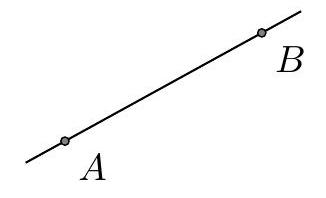
\includegraphics[max width=\textwidth, center]{2024_11_21_71f62bd117d375398909g-007}\\
różne punkty przechodzi dokładnie jedna prosta. Prostą przechodzącą przez punkty \(A\) i \(B\) będziemy oznaczali zazwyczaj \(l_{A B}\) i będziemy ją nazywali: prosta \(A B\). Zbiór tych wszystkich punktów na prostej, które leżą pomiędzy punktami \(A\) i \(B\) (wraz z punktami \(A\) i \(B\) )\\
nazywamy odcinkiem o końcach \(A, B\). Odcinek ten będziemy oznaczać \(\overline{A B}\), natomiast liczbę, która jest długością odcinka \(A B\) będziemy oznaczać \(|A B|\). Czasami będziemy tylko pisać \(A B=5\) zamiast \(|A B|=5\).

Wybrany punkt na prostej dzieli ją na dwie półproste. Półprostą o początku w punkcie \(A\) przechodzącą przez punkt \(B\) będziemy oznaczać \(A B \rightarrow\).\\
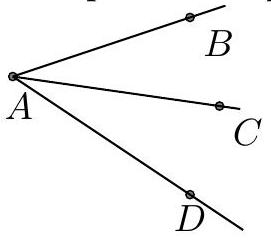
\includegraphics[max width=\textwidth, center]{2024_11_21_71f62bd117d375398909g-007(2)}

Można zwrócić uwagę na to, że po niemiecku półprosta nazywa się Strahl czyli promień światta, a po angielsku halfline lub C ray. Słowo ray znaczy promień światla. Właśnie takie określenie używane jest nie bez powodu. Spójrz na rysunek obok gdzie narysowane są trzy półproste wychodzące z punktu \(A\).\\
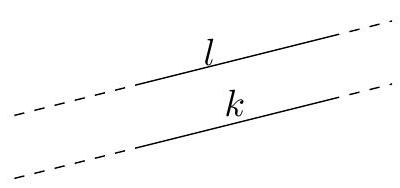
\includegraphics[max width=\textwidth, center]{2024_11_21_71f62bd117d375398909g-007(1)}

DEFINICJA Dwie proste nazywamy równoległymi, gdy nie mają żadnego punktu wspólnego (lub gdy są równe). To, że proste \(k\) i \(l\) są równoległe oznaczamy \(k \| l\).

Bardzo ważnym w naszej geometrii jest następujący

AKSJOMAT Jeżeli dany jest punkt \(P\) i prosta \(l\)\\
\((P \notin l)\), to istnieje dokładnie jedna prosta przechodząca przez punkt \(P\) i równoległa do prostej \(l\).

Właśnie z tego aksjomatu wynika, że suma wszystkich trzech kątów trójkąta jest kątem półpełnym.\\
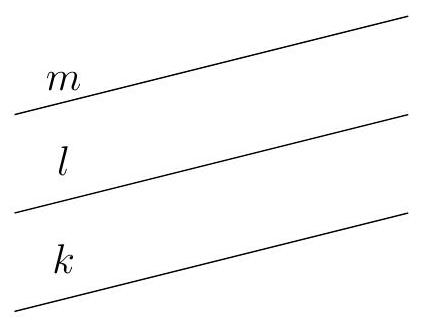
\includegraphics[max width=\textwidth, center]{2024_11_21_71f62bd117d375398909g-008}

Własność prostych równoległych:

\section*{TWIERDZENIE}
Jeżeli \(k \| l\) i \(l \| m\), to \(k \| m\).

\subsection*{1.2 Kąty}
\begin{center}
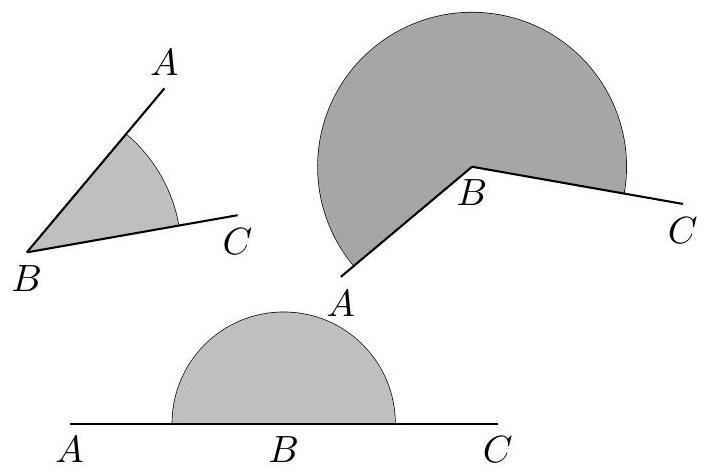
\includegraphics[max width=\textwidth]{2024_11_21_71f62bd117d375398909g-008(1)}
\end{center}

DEFINICJA Dwie półproste o wspólnym początku, wraz z jednym z dwóch obszarów, na które te półproste dzielą płaszczyznę, nazywamy katem. Kąt nazywamy pótpelnym, gdy jego ramiona są dwiema półprostymi leżącymi na jednej prostej, mającymi tylko jeden punkt wspólny.

Z każdym kątem, podobnie jak z każdym odcinkiem, związana jest liczba zwana miara kata. Kąt półpełny ma miarę \(180^{\circ}\). Jeżeli kąt półpełny podzielimy na dwa kąty o równej mierze czyli \(90^{\circ}\), to każdy taki kąt nazywamy katem prostym. Miarę kąta \(\Varangle A\) będziemy czasami oznaczać \(|\Varangle A|\). Bardzo często będziemy stosować jeden zapis dla kąta jako obiektu geometrycznego jak i dla jego miary, czyli liczby. Będziemy pisali na przykład \(\Varangle A B C=75^{\circ}\) lub też punkt \(P\) lė̇y wewnatrz kata \(\Varangle A B C\).\\
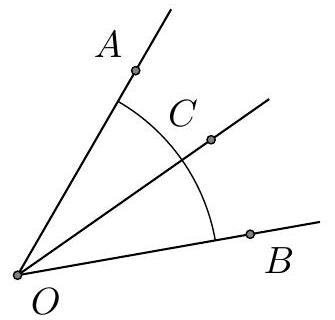
\includegraphics[max width=\textwidth, center]{2024_11_21_71f62bd117d375398909g-009(2)}

DEFINICJA Półprostą \(O C \rightarrow\) leżącą wewnątrz kata \(\Varangle A O B\) nazywamy dwusieczna kata \(\Varangle A O B\), jeżeli \(\Varangle A O C=\Varangle C O B\).

DEFINICJA Dwa kąty mniejsze od kąta półpełnego, w których jedno ramię jest wspólne, a pozostałe dwa ramiona tworzą\\
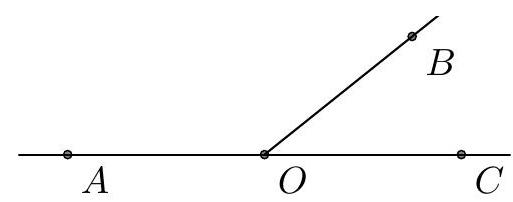
\includegraphics[max width=\textwidth, center]{2024_11_21_71f62bd117d375398909g-009}\\
jedną prostą nazywamy katami przyległymi.

DEFINICJA Każde dwa kąty, w których suma miar równa jest \(180^{\circ}\) nazywamy parą kątów dopetniajacych.

DEFINICJA Dwa kąty nieprzyległe utworzone przez dwie przecinające się proste nazywamy katami wierzchotkowymi.

TWIERDZENIE Kąty wierzchołkowe mają taką samą miarę.\\
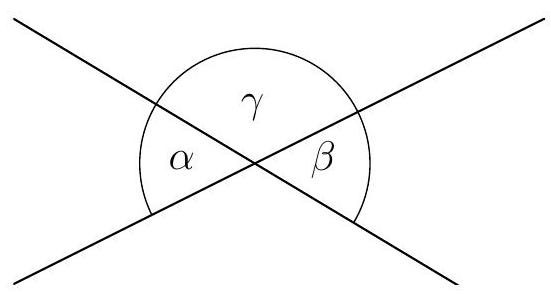
\includegraphics[max width=\textwidth, center]{2024_11_21_71f62bd117d375398909g-009(3)}

\section*{Dowód:}
Zauważmy, że\\
\(\gamma+\alpha=180^{\circ}\),\\
\(\gamma+\beta=180^{\circ}\).\\
Z powyższego wynika, że \(\alpha=\beta\).

\begin{enumerate}
  \item Na rysunku obok dany jest kąt \(\alpha\). Wyznacz \(x+y\).
  \item Uzasadnij, że dwusieczne dwóch kątów wierzchołkowych tworzą jedną prostą.
  \item Uzasadnij, że jeżeli trzy z czterech kątów jakie uzyskuje się przy przecięciu dwóch prostych mają równe miary \(\alpha\), to czwarty kąt też ma miarę \(\alpha\).\\
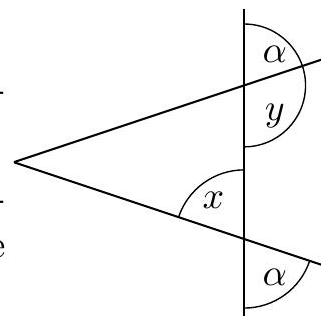
\includegraphics[max width=\textwidth, center]{2024_11_21_71f62bd117d375398909g-009(1)}
  \item Kąty \(\alpha\) i \(\beta\) są przyległe, przy czym \(\alpha: \beta=5\) : 1 (w takiej sytuacji mówimy zazwyczaj, że stosunek ich miar jest równy 5 do 1 lub, że kąt \(\alpha\) jest 5 razy większy od kąta \(\beta\) ). Wyznacz \(\alpha\) i \(\beta\).
\end{enumerate}

\subsection*{1.3 Proste prostopadłe}
DEFINICJA Jeżeli którykolwiek z czterech kątów utworzonych przez przecinające się proste \(k, l\) ma miarę \(90^{\circ}\), to proste takie nazywamy prostopadlymi i piszemy \(k \perp l\).

AKSJOMAT Jeżeli dany jest punkt \(P\) i prosta \(k\), to istnieje dokładnie jedna prosta \(l\) przechodząca przez punkt \(P\) i prostopadła do prostej \(k\).\\
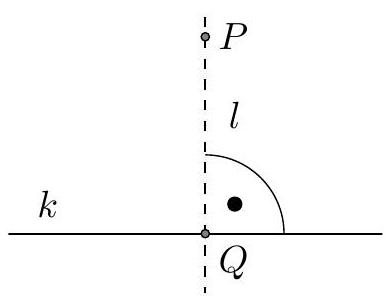
\includegraphics[max width=\textwidth, center]{2024_11_21_71f62bd117d375398909g-010}

DEFINICJA Niech dana będzie prosta \(k\) i punkt \(P\). Oznaczmy przez \(Q\) punkt przecięcia prostej \(l\) prostopadłej do \(k\) i przechodzącej przez punkt \(P\). Punkt \(Q\) nazywamy spodkiem punktu \(P\) na prostej \(k\) lub \(r z u\) tem prostopadtym punktu \(P\) na prostą \(k\). W takiej sytuacji długość odcinka \(P Q\) nazywamy odległościa punktu \(P\) od prostej \(k\) i oznaczamy \(d(P, k)\). Mamy więc \(P Q=d(P, Q)=d(P, k)\).

A oto inny aksjomat, który jest całkowicie zgodny z naszą intuicją geometryczną.\\
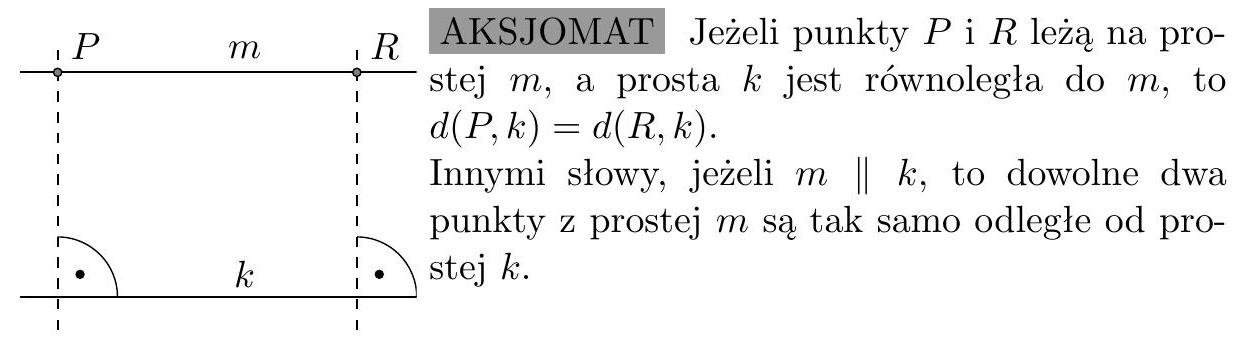
\includegraphics[max width=\textwidth, center]{2024_11_21_71f62bd117d375398909g-010(2)}

WNIOSEK: w prostokącie przeciwległe boki są równej długości.\\
5. Wyznacz w pamięci obwód obu wielokątów. Na drugim rysunku \(A B=8\), \(B C=9\).\\
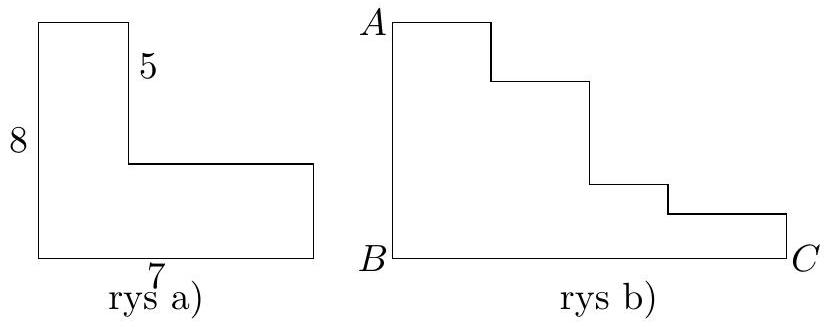
\includegraphics[max width=\textwidth, center]{2024_11_21_71f62bd117d375398909g-010(1)}\\
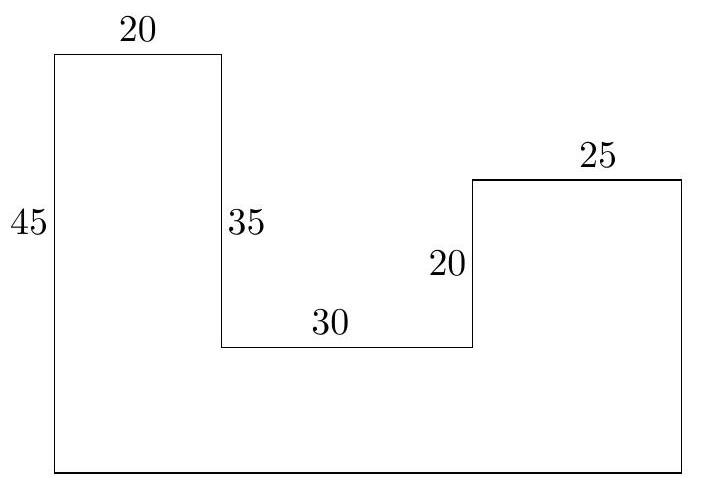
\includegraphics[max width=\textwidth, center]{2024_11_21_71f62bd117d375398909g-011(1)}\\
6. Na podstawie długości niektórych odcinków wyznacz w pamięci obwód narysowanego obok ośmiokąta.\\
7. Na podstawie długości niektórych odcinków wyznacz w pamięci obwód narysowanego obok ośmiokąta.\\
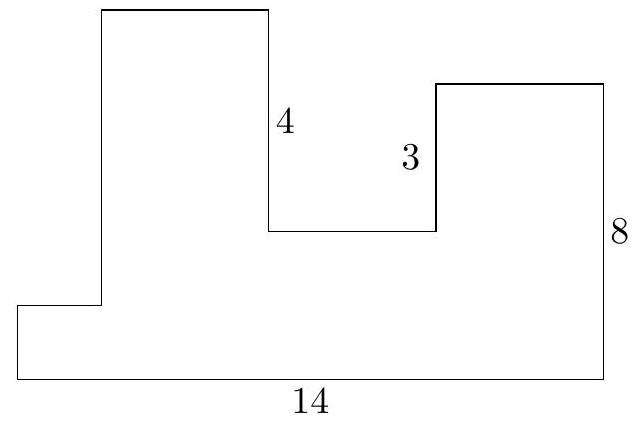
\includegraphics[max width=\textwidth, center]{2024_11_21_71f62bd117d375398909g-011(2)}

\subsection*{1.4 Kąty odpowiadające i naprzemianległe}
\begin{center}
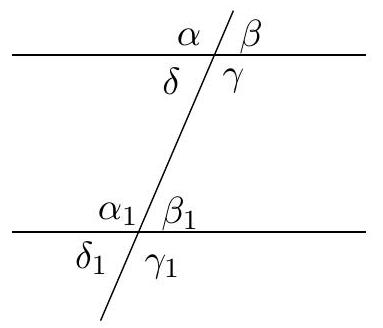
\includegraphics[max width=\textwidth]{2024_11_21_71f62bd117d375398909g-011}
\end{center}

Jeżeli dwie równoległe proste przetniemy trzecią prostą, to otrzymamy 8 kątów tak, jak na rysunku obok. Wówczas każdą z par kątów \(\left(\alpha, \alpha_{1}\right),\left(\beta, \beta_{1}\right)\), \(\left(\gamma, \gamma_{1}\right),\left(\delta, \delta_{1}\right)\) nazywamy para katów odpowiadajacych, a każdą z par \(\left(\gamma, \alpha_{1}\right),\left(\delta, \beta_{1}\right),\left(\alpha, \gamma_{1}\right),\left(\beta, \delta_{1}\right)\) nazywamy para katów naprzemianległych.

TWIERDZENIE Kąty odpowiadające mają równe miary. Kąty naprzemianległe mają równe miary.

W kolejnych zadaniach tego rozdziału możesz tylko korzystać z twierdzenia o kątach naprzemianległych i odpowiadających, z definicji kątów przyległych i własności kątów wierzchołkowych. Musisz dorysowywać proste równoległe do danych prostych. Na niektórych rysunkach takie proste równoległe są już dorysowane przerywaną kreską. Nie możesz korzystać z sumy kątów trójkąta.\\
8. Na poniższych rysunkach \(k \| l\). Wyznacz \(x\). Na niektórych rysunkach masz już dorysowane kropkowaną linią proste równoległe do prostych \(k\) i \(l\). Na pozostałych rysunkach musisz to sam zrobić.\\
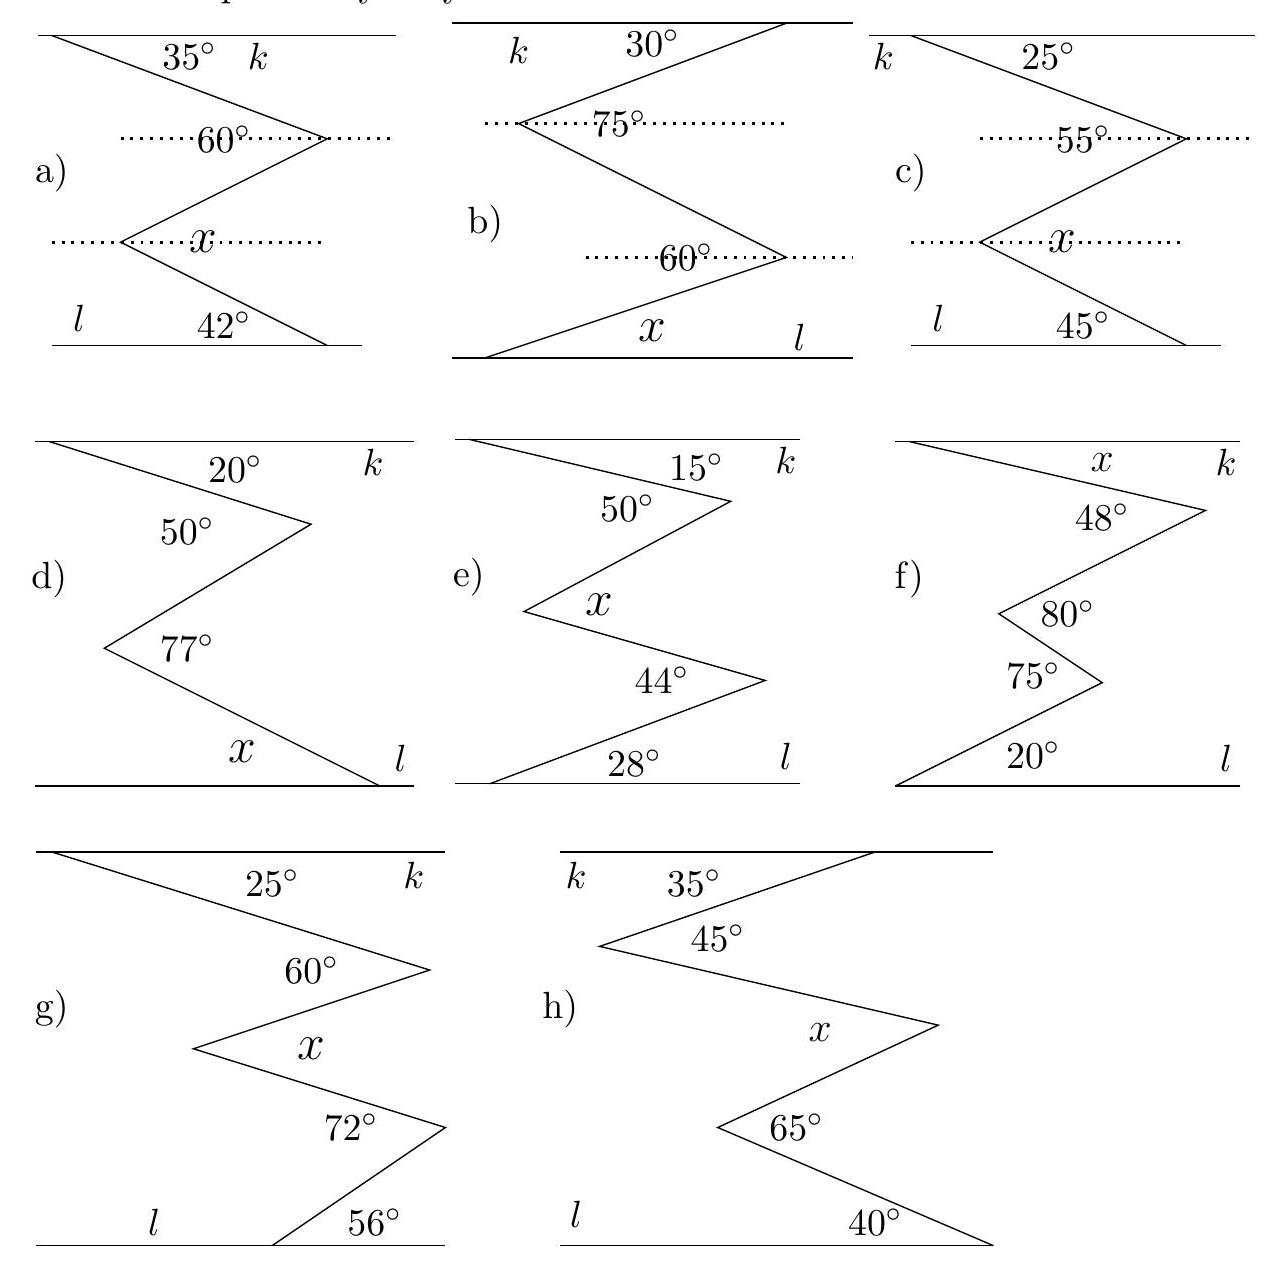
\includegraphics[max width=\textwidth, center]{2024_11_21_71f62bd117d375398909g-012(2)}\\
9. Na poniższych rysunkach \(k \| l\). Wyznacz \(x+y\).\\
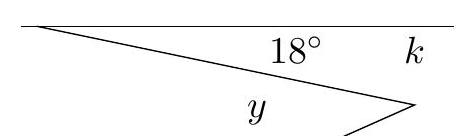
\includegraphics[max width=\textwidth, center]{2024_11_21_71f62bd117d375398909g-012}\\
a)\\
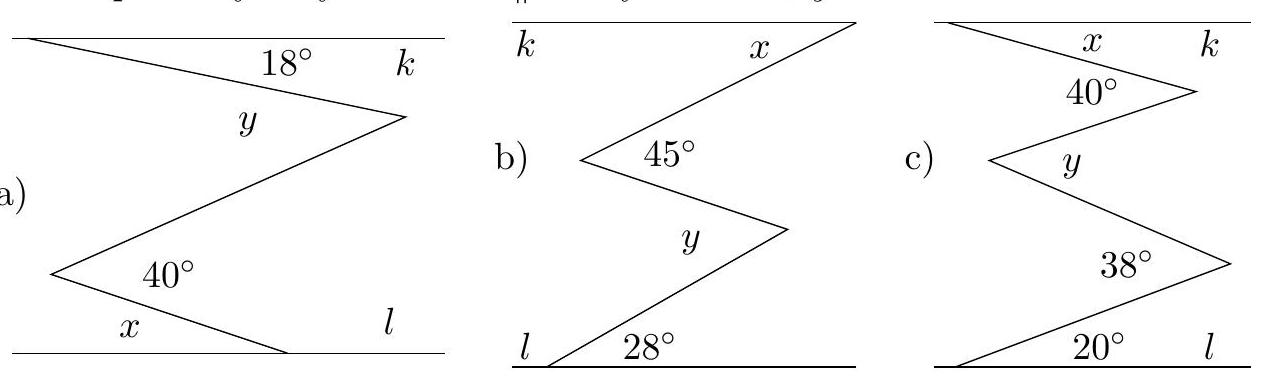
\includegraphics[max width=\textwidth, center]{2024_11_21_71f62bd117d375398909g-012(1)}\\
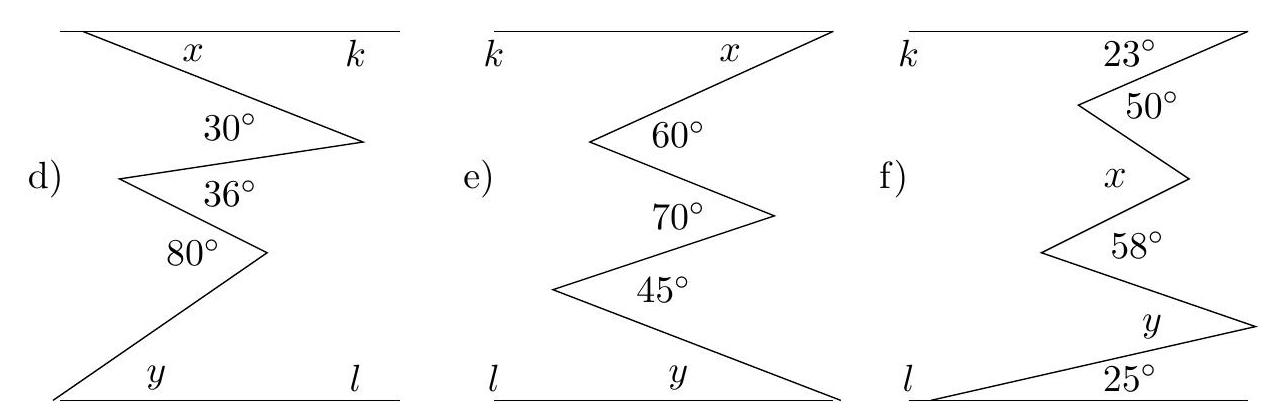
\includegraphics[max width=\textwidth, center]{2024_11_21_71f62bd117d375398909g-013(1)}\\
10. Wyznacz \(\alpha\) na rysunku obok.\\
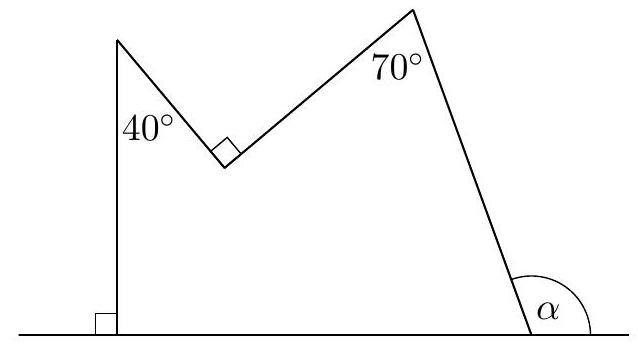
\includegraphics[max width=\textwidth, center]{2024_11_21_71f62bd117d375398909g-013}\\
11. Na poniższych rysunkach \(k \| l\). Na podstawie podanych miar kątów wyznacz \(x\), względnie \(x\) i \(y\). Na pierwszym rysunku zostały już narysowane przerywana kreską proste równoległe do prostych \(k\) i \(l\).\\
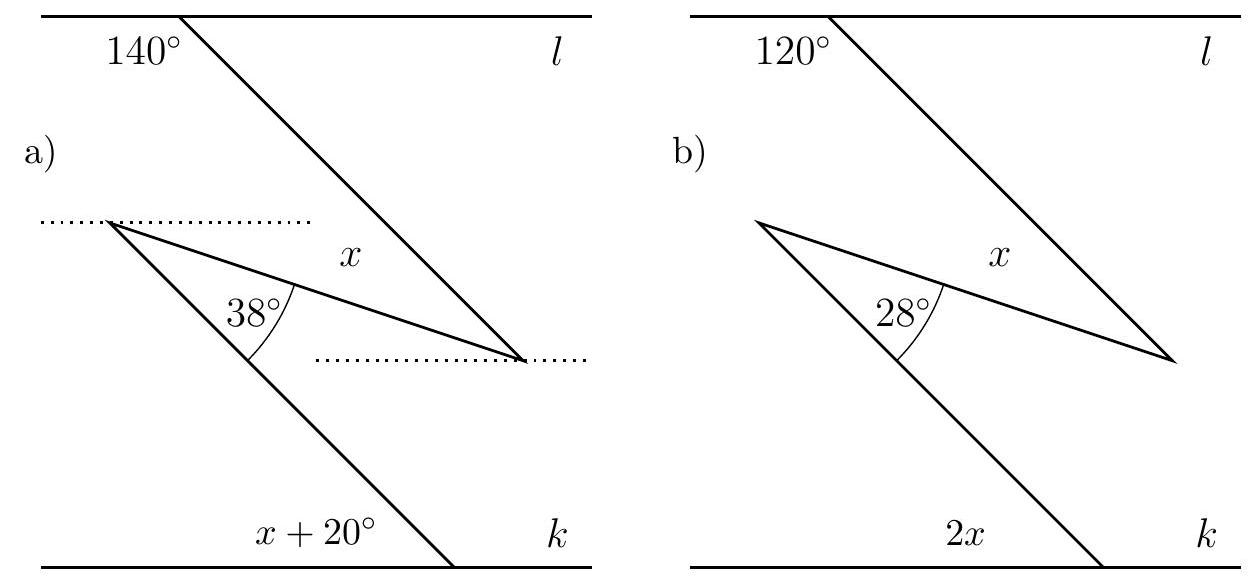
\includegraphics[max width=\textwidth, center]{2024_11_21_71f62bd117d375398909g-013(2)}\\
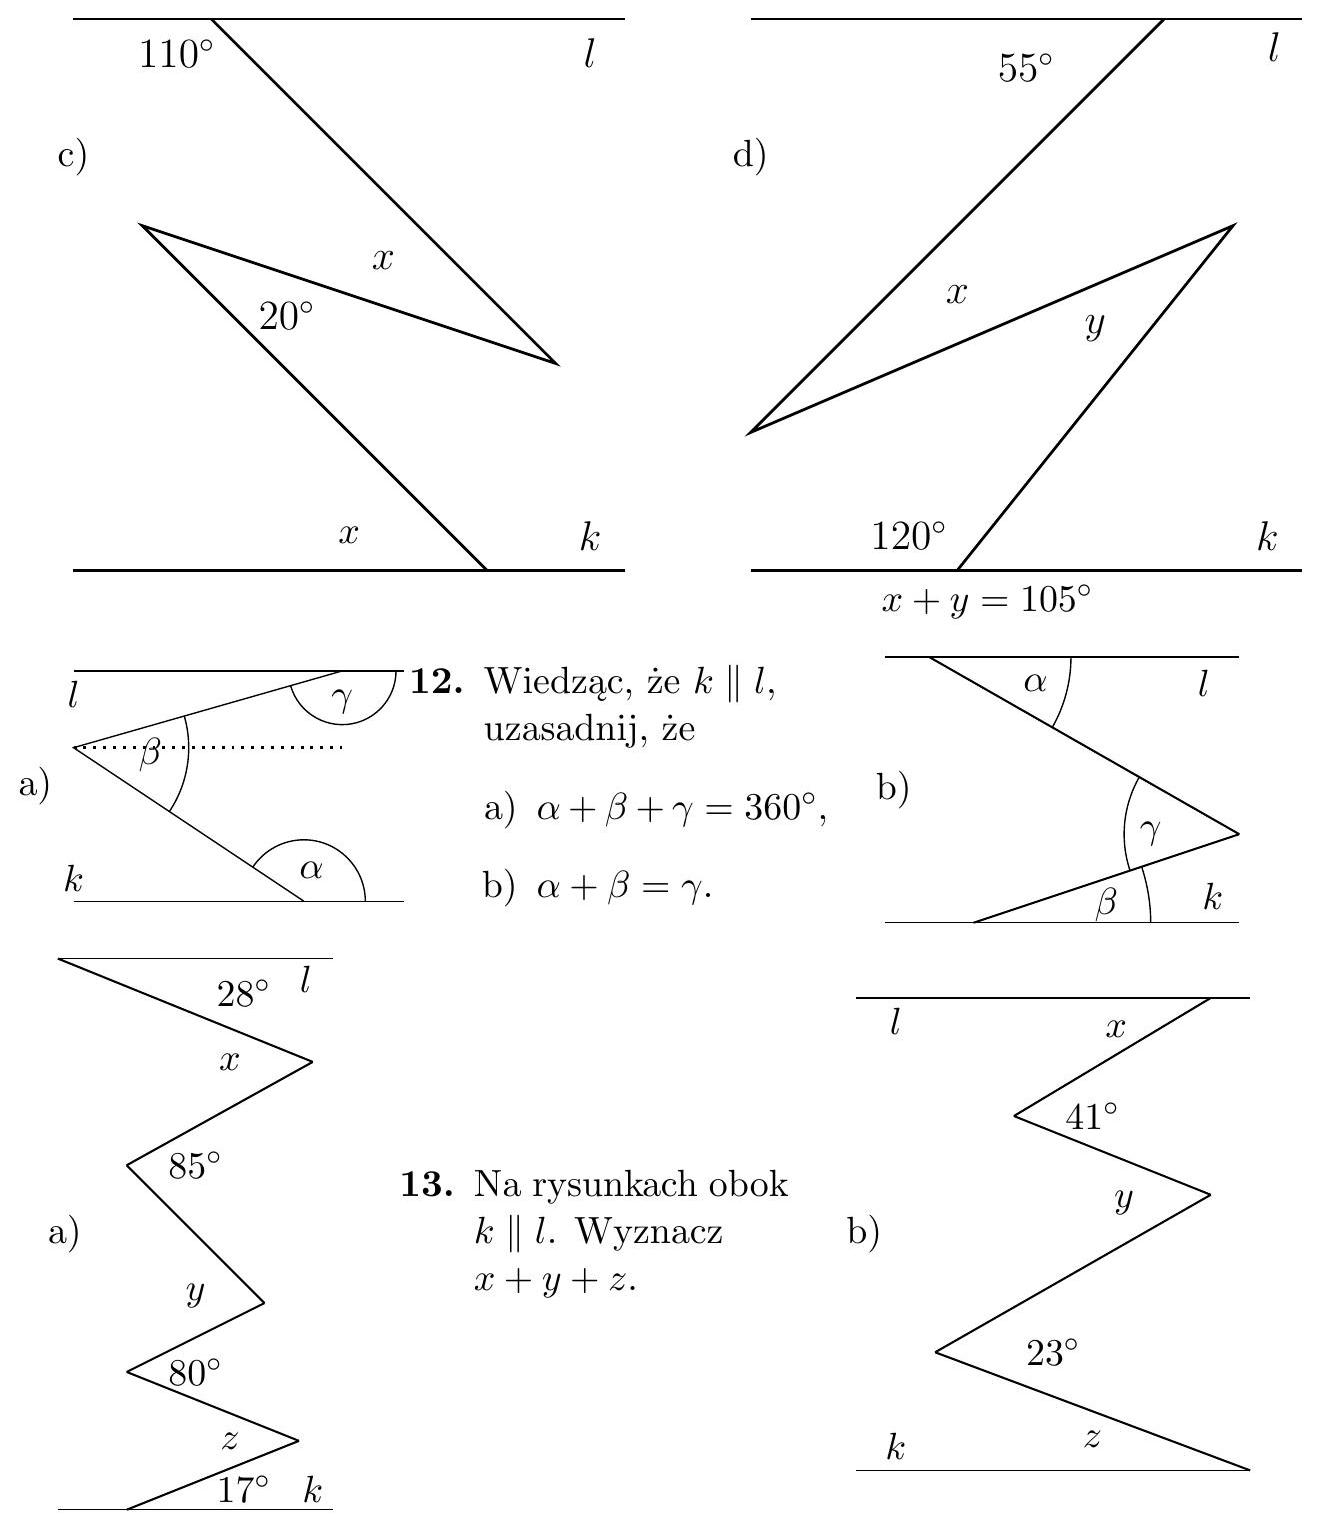
\includegraphics[max width=\textwidth, center]{2024_11_21_71f62bd117d375398909g-014(1)}\\
14. Wiedząc, że \(k \| l\), \(m \| n\), wyznacz \(x\) i \(y\) 。\\
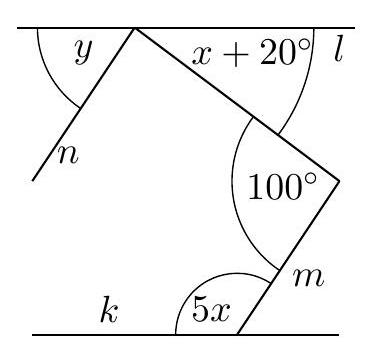
\includegraphics[max width=\textwidth, center]{2024_11_21_71f62bd117d375398909g-014}\\
15. Wiedząc, że \(\overline{C L} \| \overline{A B}\).

Uzasadnij, że \(\delta=\alpha+\beta\).\\
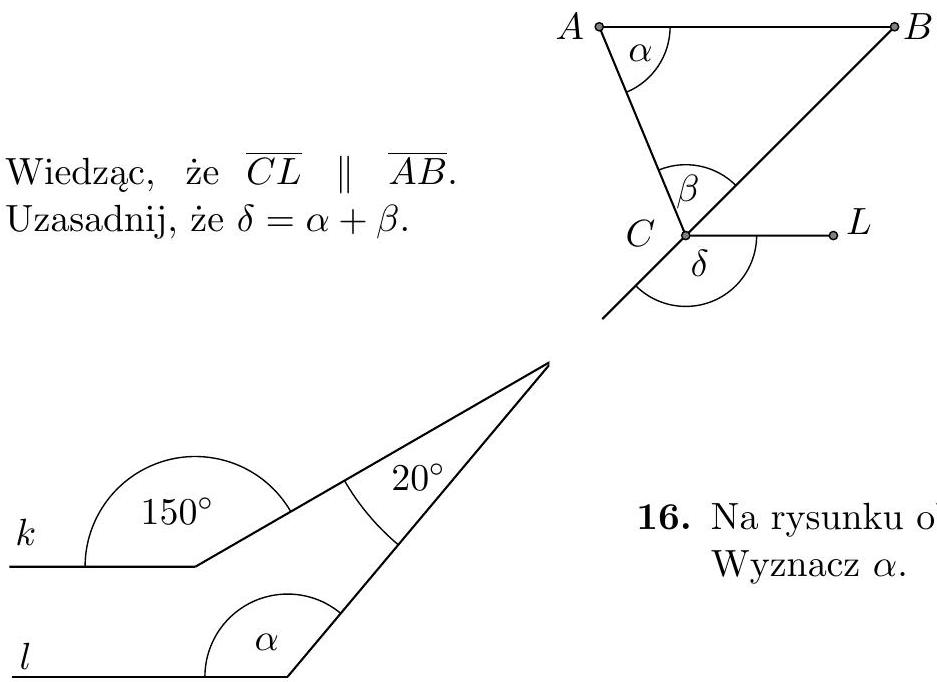
\includegraphics[max width=\textwidth, center]{2024_11_21_71f62bd117d375398909g-015(1)}\\
16. Na rysunku obok \(k \| l\).

Wyznacz \(\alpha\).\\
17. Na poniższych rysunkach \(k \| l\), dodatkowo na drugim rysunku \(p \| q\). Wyznacz \(x+y+z\) na pierwszym rysunku oraz \(\alpha\) i \(\beta\) na drugim rysunku. W celu ułatwienia sobie rozwiązania zadania sporządź rysunki w zeszycie powiększając je.\\
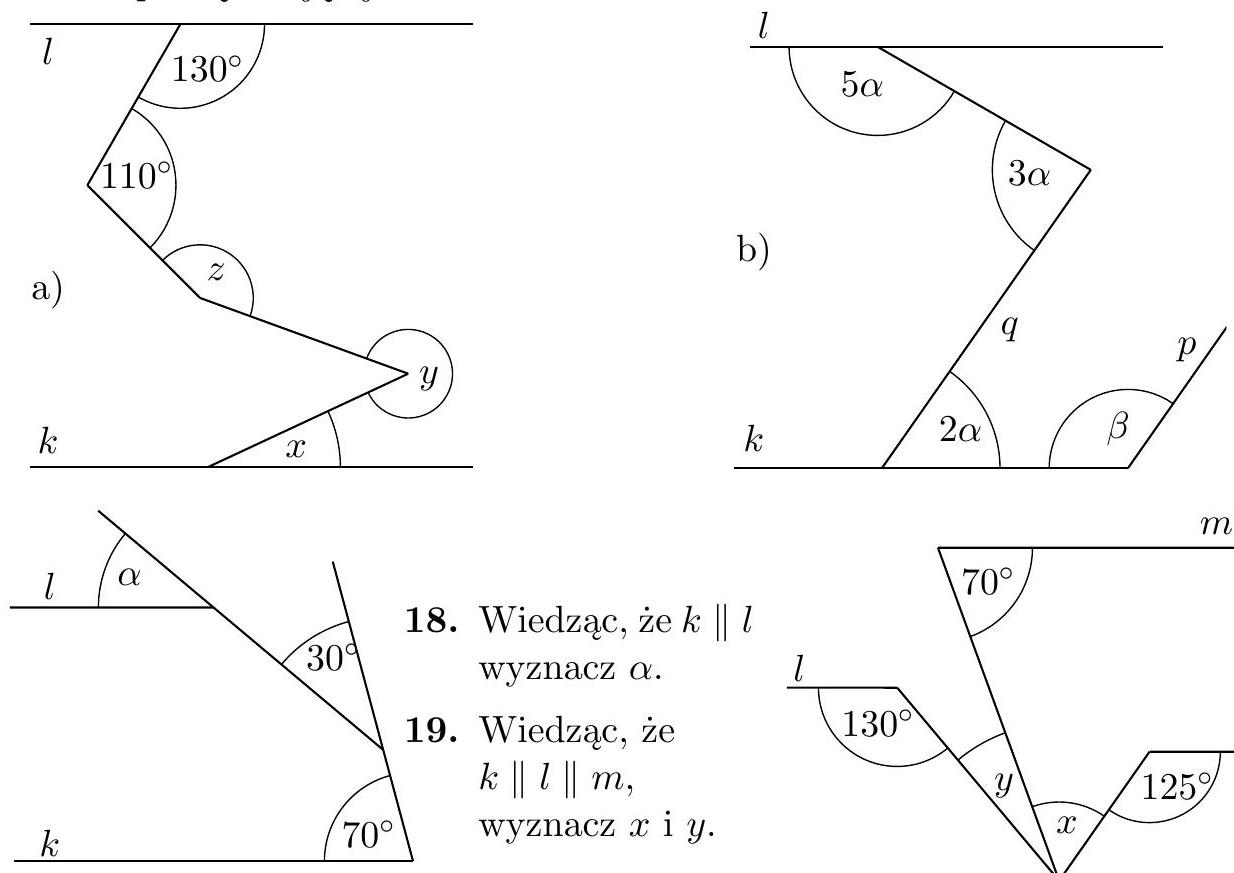
\includegraphics[max width=\textwidth, center]{2024_11_21_71f62bd117d375398909g-015(2)}\\
18. Wiedząc, że \(k \| l\) wyznacz \(\alpha\).\\
19. Wiedząc, że \(k\|l\| m\), wyznacz \(x\) i \(y\).\\
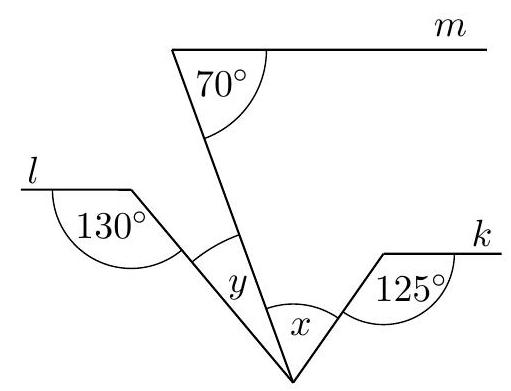
\includegraphics[max width=\textwidth, center]{2024_11_21_71f62bd117d375398909g-015}

DEFINICJA Czworokąt, w którym boki są parami równoległe, nazywamy równoległobokiem.\\
\(!\Rightarrow\) 20. Uzasadnij, że w równoległoboku kąty leżące na przeciwko siebie mają równe miary.

\section*{Wskazówki i odpowiedzi.}
\begin{enumerate}
  \item \(180^{\circ}\)
  \item wsk. zobacz definicję kąta półpełnego oraz kątów wierzchołkowych
  \item wsk. zobacz definicję kąta półpełnego oraz kątów wierzchołkowych
  \item \(\alpha=150^{\circ}, \beta=30^{\circ}\)
  \item a) 30, b) 34
  \item 280\\
7.52
  \item a) \(67^{\circ}\), b) \(15^{\circ}\), c) \(75^{\circ}\), d) \(47^{\circ}\),\\
e) \(51^{\circ}\), f) \(23^{\circ}\), g) \(51^{\circ}\), h) \(35^{\circ}\)
  \item a) \(58^{\circ}\), b) \(73^{\circ}\), c) \(58^{\circ}\), d) \(74^{\circ}\),\\
e) \(35^{\circ}\), f) \(110^{\circ}\)
  \item \(\alpha=110^{\circ}\).
  \item a) \(29^{\circ}\), b) \(29 \frac{1}{3}^{\circ}\), c) \(45^{\circ}\),\\
d) \(x=50^{\circ}, y=55^{\circ}\)
  \item a) \(x+y+z=210^{\circ}\),\\
b) \(x+y+z=64^{\circ}\)
  \item a) \(x=50^{\circ}, y=115^{\circ}\),\\
b) \(x=25^{\circ}, y=55^{\circ}\)
  \item wsk. przedłuż prostą \(C L\)
  \item \(\alpha=130^{\circ}\)
  \item a) \(x+y+z=480^{\circ}\),\\
b) \(\alpha=30^{\circ}, \beta=120^{\circ}\)
  \item \(\alpha=40^{\circ}\) wsk. poprowadź odpowiednią prostą równoległą
  \item \(x=55^{\circ}, y=20^{\circ}\) wsk. przedłuż jedną z trzech prostych równoległych i dorysuj jeszcze jedną prostą równoległą
\end{enumerate}

\section*{Rozdział 2}
\section*{SUMA KĄTÓW TRÓJKĄTA}
\subsection*{2.1 Kąty (wewnętrzne) w trójkącie}
Wpierw udowodnimy twierdzenie o sumie kątów dowolnego trójkąta.\\
TWIERDZENIE Suma miar kątów dowolnego trójkąta wynosi \(180^{\circ}\).

\section*{Dowód:}
Niech dany będzie dowolny trójkąt \(A B C\). Przez punkt \(C\) prowadzimy prostą \(k\) równoległą do podstawy \(A B\). Taka prosta jest dokładnie jedna. Teraz już wystarczy tylko spojrzeć na rysunek, zobaczyć pary kątów naprzemianległych i widać, że suma wszystkich trzech kątów trójkąta jest\\
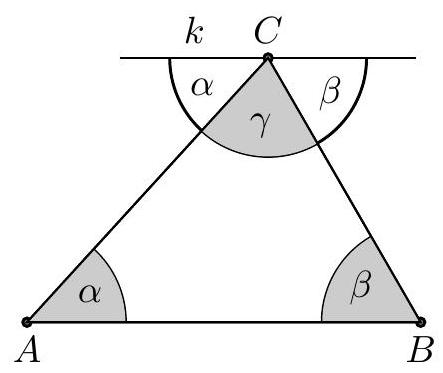
\includegraphics[max width=\textwidth, center]{2024_11_21_71f62bd117d375398909g-017}\\
równa kątowi półpełnemu.

WNIOSEK Suma kątów czworokąta jest równa \(360^{\circ}\). Wynika to z tego, że czworokąt można podzielić przekątną na dwa trójkąty.

DEFINICJA Trójkąt w którym wszystkie kąty są ostre nazywamy trójkatem ostrokatnym. Trójkąt, w którym jeden kąt jest rozwarty nazywamy trójkatem rozwartokatnym. Trójkąt, w którym jeden z kątów jest prosty nazywamy trójkatem prostokatnym. Boki wychodzące z wierzchołka kąta prostego nazywamy przyprostokątnymi, zaś bok leżący na przeciwko kąta prostego nazywamy przeciwprostokatna.

\section*{PRZYKŁAD}
Oblicz kąty ostre trójkąta prostokątnego, w którym jeden z kątów ostrych jest o \(26^{\circ}\) większy od drugiego kąta ostrego.\\
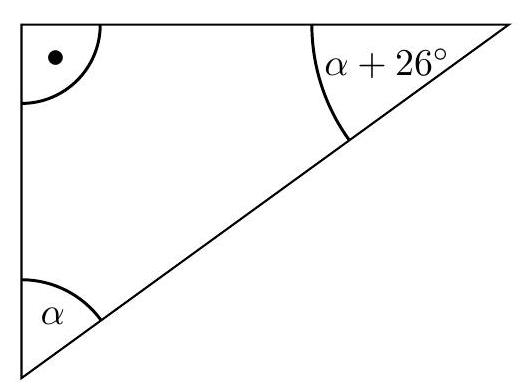
\includegraphics[max width=\textwidth, center]{2024_11_21_71f62bd117d375398909g-018}

Przy oznaczeniach jak na rysunku obok mamy

\[
\begin{aligned}
\alpha+\alpha+26^{\circ} & =90^{\circ} \\
2 \alpha & =64^{\circ} \\
\alpha & =32^{\circ}
\end{aligned}
\]

Zatem kąty ostre trójkąta mają \(32^{\circ}\) i \(58^{\circ}\).

\begin{enumerate}
  \item Jeden z kątów trójkąta jest równy \(25^{\circ}\), a różnica pozostałych wynosi \(15^{\circ}\). Wyznacz te kąty.
  \item Jeden z kątów trójkąta równa się różnicy dwóch pozostałych kątów. Wyznacz miarę największego kąta w tym trójkącie.
  \item Oblicz kąty trójkąta, w którym jeden kąt jest dwa razy większy od drugiego, a trzeci kąt jest równy sumie dwóch pozostałych.
  \item Stosunek miar dwóch kątów w trójkącie \(\alpha\) i \(\beta\) wynosi \(4: 5\) co oznacza, że \(\alpha: \beta=4: 5\), zaś trzeci, największy kąt, jest większy od najmniejszego o \(37^{\circ}\). Wyznacz kąty tego trójkąta.
  \item Wyznacz kąty w trójkącie, jeżeli stosunek ich miar wynosi \(5: 3: 1\).\\
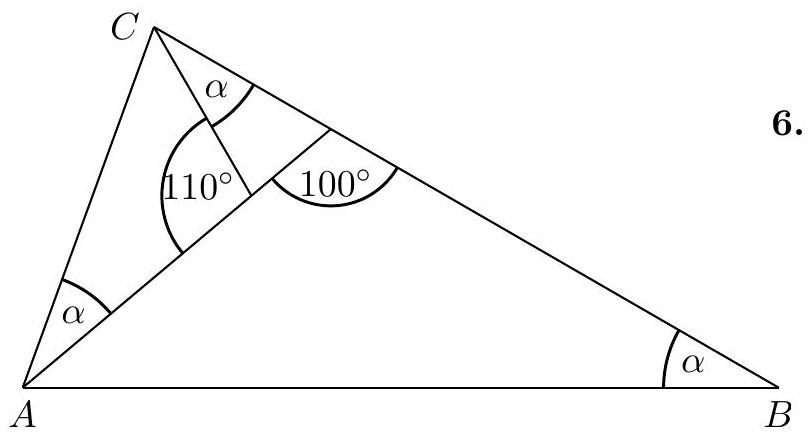
\includegraphics[max width=\textwidth, center]{2024_11_21_71f62bd117d375398909g-018(1)}
  \item Na podstawie podanych miar dwóch kątów, wiedząc że trzy kąty mają miarę \(\alpha\), wyznacz \(\alpha\) oraz miary kątów w trójkącie \(A B C\).
  \item W trójkącie ostrokątnym \(A B C\) opuszczono z wierzchołka \(C\) wysokość \(C C^{\prime}\). Wyznacz miary kątów \(A C C^{\prime}\) i \(B C C^{\prime}\), jeżeli \(\Varangle A=70^{\circ}, \Varangle C=48^{\circ}\). (przypomnijmy, że wysokość trójkąta jest to odcinek łączący wierzchołek trójkąta z prostą wyznaczoną przez pozostałe dwa wierzchołki i prostopadły do tej prostej).\\
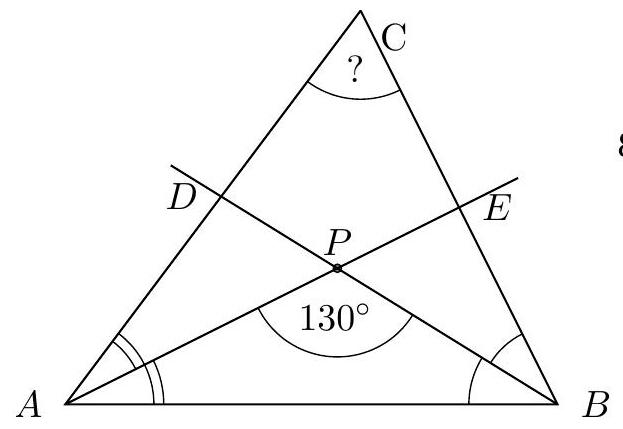
\includegraphics[max width=\textwidth, center]{2024_11_21_71f62bd117d375398909g-019(2)}
  \item Na rysunku obok \(B D\) i \(A E\) są dwusiecznymi kątów. Miara kąta \(A P B\) jest równa \(130^{\circ}\). Wyznacz miarę kąta \(A C B\). Wsk. oznacz \(\Varangle C A B=2 \alpha, \Varangle C B A=2 \beta\).
  \item W trójkącie \(A B C\) na rysunku obok \(\Varangle C=70^{\circ}, A P\) jest dwusieczną kąta \(A\), zaś \(B P\) jest dwusieczną kąta \(B\). Wyznacz \(\Varangle A P B\).\\
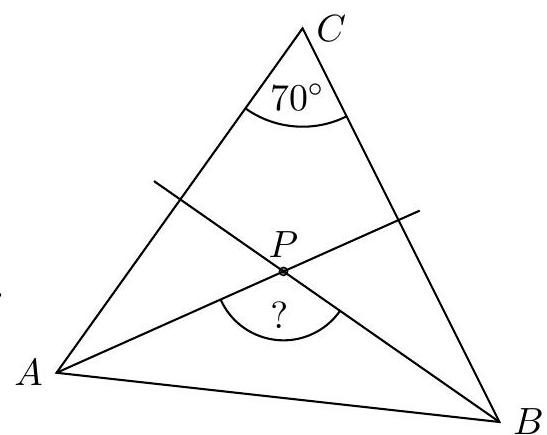
\includegraphics[max width=\textwidth, center]{2024_11_21_71f62bd117d375398909g-019(1)}
  \item W trójkącie prostokątnym \(A B C\) kąt przy wierzchołku \(C\) jest prosty, zaś jeden z kątów ostrych ma miarę \(\alpha\) (jeżeli to ci ułatwi obliczenia przyjmij, że \(\alpha=38^{\circ}\) ). Wyznacz miarę kąta (rozwartego) pod jakim przecinają się dwusieczne kątów ostrych w tym trójkącie.\\
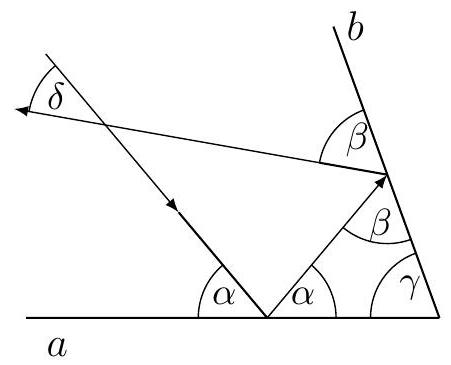
\includegraphics[max width=\textwidth, center]{2024_11_21_71f62bd117d375398909g-019}
  \item Na rysunku obok \(a\) i \(b\) oznaczają powierzchnie dwóch zwierciadeł, strzałki oznaczają drogę promienia światła padającego na zwierciadło \(a\). Wyznacz kąt \(\delta\) gdy:\\
a) \(\alpha=70^{\circ}, \gamma=60^{\circ}\),\\
b) \(\gamma=60^{\circ}\), zaś \(\alpha\) jest dowolnym - co oznacza „nie ustalonym" - kątem.\\
c) \(\gamma=70^{\circ}\), zaś \(\alpha\) jest dowolnym kątem.
  \item W trójkącie prostokątnym \(A B C\) kąt ostry przy wierzchołku \(A\) ma miarę \(\alpha\). (jeżeli to ci ułatwi obliczenia, to przyjmij, że \(\alpha=32^{\circ}\) ). Wysokość \(C C^{\prime}\) wychodzi z wierzchołka kąta prostego. Wyznacz kąt pod jakim przecinają się dwusieczne kątów \(A C C^{\prime}\) i \(C B C^{\prime}\).
  \item W trójkącie \(A B C\) dwusieczna kąta \(A\) jest prostopadła do boku \(B C\), zaś dwusieczna kąta \(B\) jest prostopadła do boku \(A C\). Uzasadnij, że w tym trójkącie każdy kąt ma \(60^{\circ}\).\\
\(!\Rightarrow\) 14. Uzasadnij, że dwa kąty o ramionach wzajemnie prostopadłych mają równe miary\\
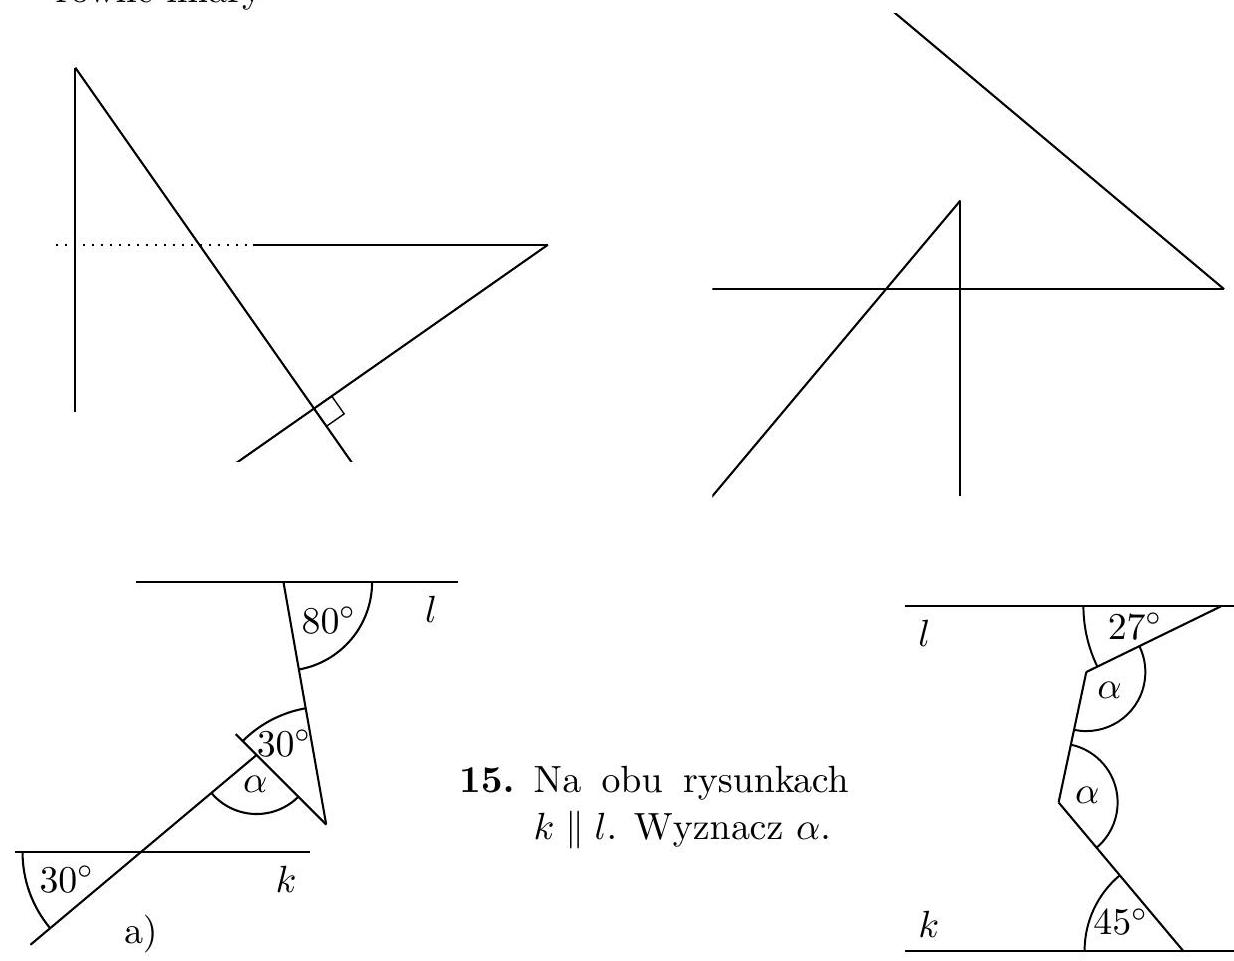
\includegraphics[max width=\textwidth, center]{2024_11_21_71f62bd117d375398909g-020(2)}
  \item Na obu rysunkach \(k \| l\). Wyznacz \(\alpha\).\\
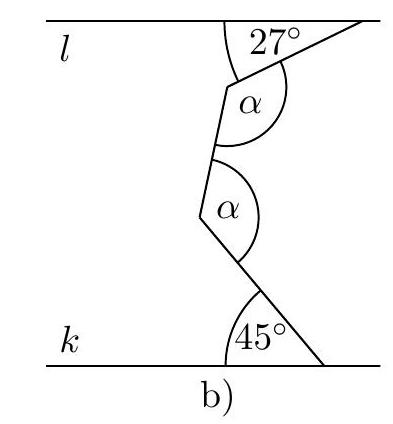
\includegraphics[max width=\textwidth, center]{2024_11_21_71f62bd117d375398909g-020}
  \item Na rysunku obok \(l_{1} \| l_{2}, \overline{X Y} \perp l_{1}\), zaś \(\overline{A B} \perp l_{2}\). Uzasadnij, że \(\alpha=\beta\).
  \item Uzasadnij, że dwusieczne kątów przyległych tworzą kąt prosty. Pamiętaj, że kąty przyległe mają jedno ramię wspólne, a kąty te tworzą razem kąt półpełny.\\
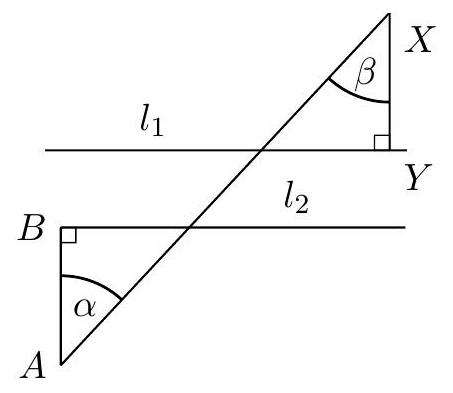
\includegraphics[max width=\textwidth, center]{2024_11_21_71f62bd117d375398909g-020(1)}
  \item W równoległoboku \(A B C D\) kąt przy wierzchołku \(D\) jest rozwarty. Z punktu \(D\) poprowadzono dwie wysokości równoległoboku, tworzące kąt \(\alpha\). Uzasadnij, że kąt ostry równoległoboku jest równy \(\alpha\). Przypomnijmy, że wysokość w równoległoboku jest to odcinek łączący parę prostych równoległych przechodzących przez boki równoległoboku i prostopadły do tych prostych.
  \item Na rysunku obok \(a \| b\). Półproste \(M O^{\rightarrow} \mathrm{i}\) \(E O \rightarrow\) są dwusiecznymi wskazanych kątów. Uzasadnij, że \(\Varangle M O E=90^{\circ}\).\\
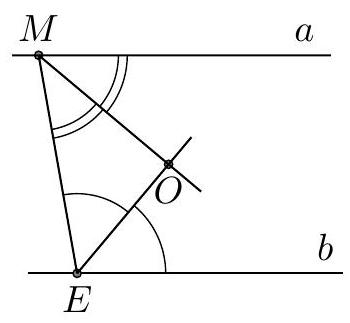
\includegraphics[max width=\textwidth, center]{2024_11_21_71f62bd117d375398909g-021}
  \item W trójkącie \(A B C\) kąty \(\Varangle A\) i \(\Varangle B\) są równe. Dwusieczna \(A D\) tworzy z bokiem \(B C\) kąt \(60^{\circ}\). Wyznacz miary kątów tego trójkąta. Zauważ, że tak sformułowane zadanie ma dwa rozwiązania. Zrób odpowiednie rysunki.
\end{enumerate}

21* Uzasadnij, ze w trójkącie \(A B C\) kąt pomiędzy wysokością wychodzącą z wierzchołka \(A\) i dwusieczną kąta \(A\) jest równy połowie różnicy dwóch pozostałych kątów.\\
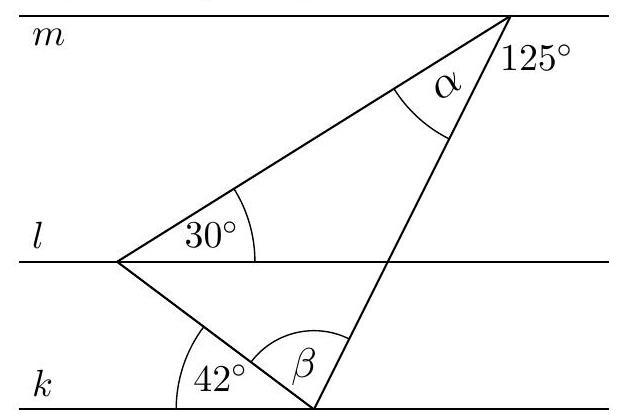
\includegraphics[max width=\textwidth, center]{2024_11_21_71f62bd117d375398909g-021(2)}\\
22. Na rysunku obok \(k\|l\| m\). Wyznacz \(\alpha\) i \(\beta\).

\subsection*{2.2 Kąty zewnętrzne w trójkącie}
Wygodnym pojęciem, którego będziemy wielokrotnie używali, jest: kat zewnętrzny w trójkacie.

DEFINICJA Kąt przyległy do kąta (wewnętrznego) w trójkącie nazywamy kątem zewnętrznym. Na przykład w trójkącie \(A B C\) na rysunku obok \(\alpha\) jest kątem wewnętrznym zaś \(\alpha^{\prime}\) i \(\alpha^{\prime \prime}\) są kątami zewnętrznymi przy wierzchołku \(A\).\\
UWAGA Każdy kąt wewnętrzny w trójkącie ma dwa przyległe do niego kąty zewnętrzne czyli w każdym trójkącie jest sześć kątów zewnętrznych.\\
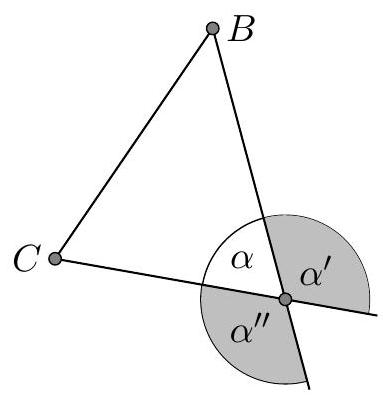
\includegraphics[max width=\textwidth, center]{2024_11_21_71f62bd117d375398909g-021(1)}

Ma miejsce przy tym następujące TWIERDZENIE Kąt zewnętrzny w trójkącie równy jest sumie tych dwóch kątów wewnętrznych trójkąta, które do niego nie przylegają, czyli, że przy oznaczeniach jak na rysunku obok

\[
\alpha^{*}=\beta+\gamma
\]

\begin{center}
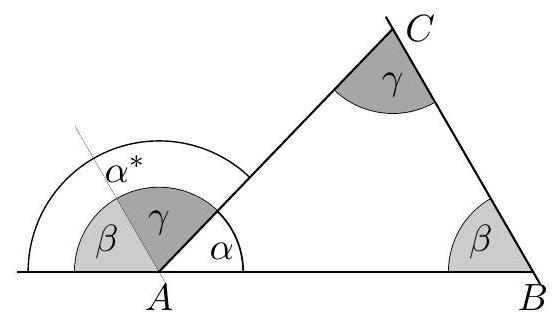
\includegraphics[max width=\textwidth]{2024_11_21_71f62bd117d375398909g-022}
\end{center}

\section*{Dowód:}
Rozważmy kąt zewnętrzny \(\alpha^{*}\) trójkąta \(A B C\), w którym kąty wewnętrzne mają miary \(\alpha, \beta\) i \(\gamma\). Przez punkt \(A\) poprowadziliśmy prostą równoległą do prostej \(B C\). Taka prosta jest tylko jedna, co wynika z przytoczonego na początku kursu aksjomatu. Z tego, że te proste są równoległe wynika równość odpowiednich kątów naprzemianległych i odpowiadających, co zostało zaznaczone na rysunku. Ponieważ w każdym trójkącie \(\alpha+\beta+\gamma=180^{\circ}\), a przy \(\operatorname{tym} \alpha+\alpha^{*}=180^{\circ}\) - jako kąty przyległe, wobec tego \(\alpha^{*}=\beta+\gamma\).\\
Zauważmy dodatkowo, że ponieważ \(\beta\) i \(\gamma\) są liczbami dodatnimi, to z powyższej równości wynika, że

\[
\alpha^{*}>\beta \quad \mathrm{i} \quad \alpha^{*}>\gamma
\]

Co możemy sformułować jako\\
WNIOSEK (z którego nie raz będziemy korzystać) Kąt zewnętrzny w trój-\\
\(!\Rightarrow\) kącie jest większy od każdego z tych kątów wewnętrznych trójkąta, które do niego nie przylegają.\\
23. Cztery kąty zewnętrzne w trójkącie mają po \(150^{\circ}\). Po ile stopni mają pozostałe dwa kąty zewnętrzne?\\
24. Uzasadnij, że suma wszystkich sześciu kątów zewnętrznych trójkąta wynosi \(720^{\circ}\).\\
25. W trójkącie \(A B C\) kąt zewnętrzny przy wierzchołku \(A\) ma \(40^{\circ}\). Z wierzchołków \(B\) i \(C\) poprowadzono wysokości tego trójkąta. Wyznacz miarę kąta ostrego pomiędzy prostymi zawierajaccymi te dwie wysokości.\\
26. W trójkącie \(A B C\) poprowadzono z wierzchołka \(C\) dwusieczne kątów: wewnętrznego i zewnętrznego. Dwusieczna \(C D\) kąta wewnętrznego tworzy z bokiem \(A B\) kąt \(126^{\circ}\). Dwusieczna kąta zewnętrznego przecina prostą\\
\(A B\) w punkcie \(E\). Wyznacz miarę kąta \(C E B\). Wsk. por. zad. 17\\
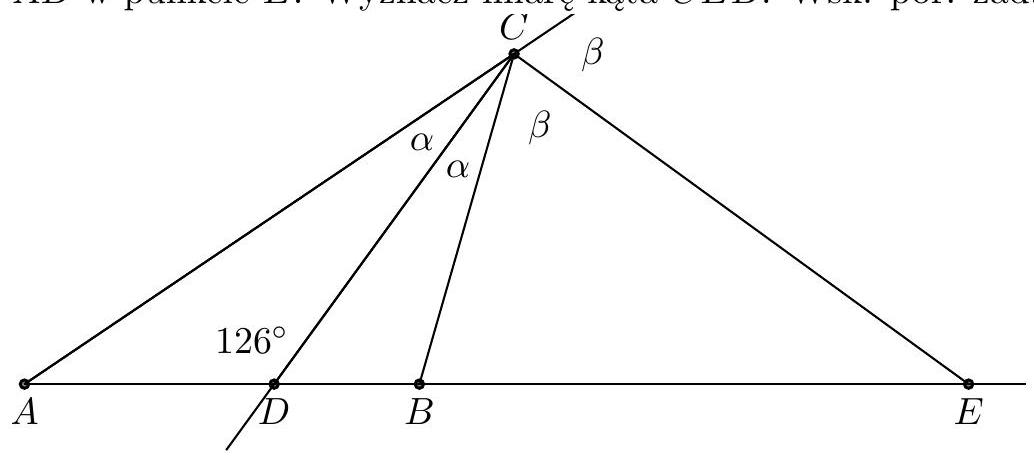
\includegraphics[max width=\textwidth, center]{2024_11_21_71f62bd117d375398909g-023(1)}

\section*{PRZYKŁAD}
W trójkącie suma kątów \(\alpha\) i \(\beta\) równa jest kątowi \(\gamma\). Wyznacz miarę kąta \(\gamma\).\\
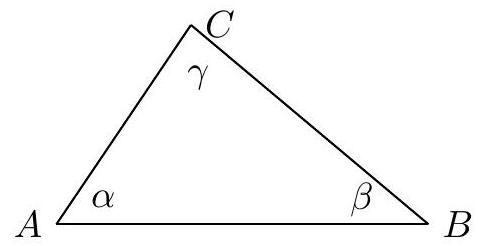
\includegraphics[max width=\textwidth, center]{2024_11_21_71f62bd117d375398909g-023}

\section*{Rozwiązanie}
Suma kątów trójkąta jest równa \(180^{\circ}\), wobec tego mamy

\[
\alpha+\beta+\gamma=180^{\circ}
\]

Ponieważ

\[
\alpha+\beta=\gamma
\]

wobec tego mamy

\[
\alpha+\beta+\gamma=\alpha+\beta+\underbrace{\alpha+\beta}_{=\gamma}=180^{\circ}
\]

czyli

\[
2 \alpha+2 \beta=180^{\circ} \quad \text { zaś } \quad \alpha+\beta=90^{\circ}
\]

Zatem \(\gamma=90^{\circ}\)\\
27. Postępując w podobny sposób wyznacz miarę kąta \(\gamma\) gdy w trójkącie o kątach \(\alpha, \beta, \gamma\) suma kątów \(\alpha\) i \(\beta\) jest\\
a) równa połowie kąta \(\gamma\)\\
b) równa jednej trzeciej kąta \(\gamma\)\\
c) dwa razy większa od kąta \(\gamma\)\\
d) pięć razy większa od kąta \(\gamma\)\\
e) o \(60^{\circ}\) większa od kąta \(\gamma\)\\
f) o \(30^{\circ}\) mniejsza od kąta \(\gamma\)\\
28. W trójkącie prostokątnym \(A B C\) dwusieczna kąta prostego tworzy z wysokością poprowadzoną z tego samego wierzchołka kąt o mierze \(12^{\circ}\). Wyznacz miary kątów ostrych w trójkącie \(A B C\).\\
29. Największy kąt w trójkącie ma \(82^{\circ}\), a najmniejszy \(45^{\circ}\). Z wierzchołków dwóch mniejszych kątów poprowadzono wysokości trójkąta. Wyznacz miarę kąta ostrego pomiędzy tymi wysokościami.

\section*{PRZYKŁAD}
W trójkącie ostrokątnym \(A B C\) dane są miary kątów: \(\Varangle A=\alpha, \Varangle B=\beta\), \(\Varangle C=\gamma\). Wyznacz miarę kąta rozwartego pomiędzy dwusiecznymi kątów \(A\) i \(B\) w zależności od \(\gamma\).\\
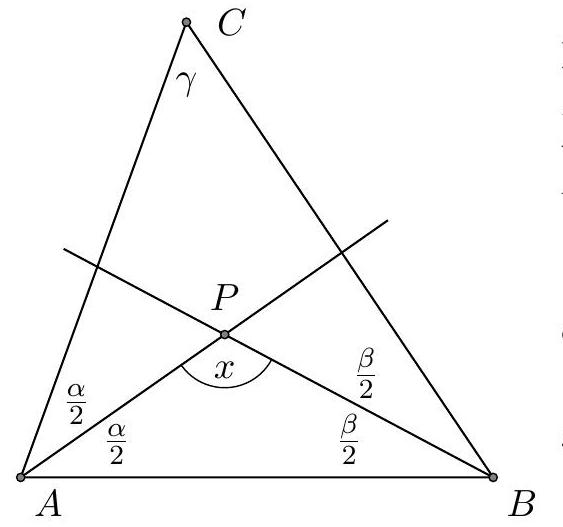
\includegraphics[max width=\textwidth, center]{2024_11_21_71f62bd117d375398909g-024}

Niech \(A P\) będzie dwusieczną kąta \(B A C\), \(B P\) dwusieczną kąta \(A B C\), zaś \(x\) poszukiwanym kątem. W trójkącie \(A B P\) mamy zatem

\[
x+\frac{\alpha}{2}+\frac{\beta}{2}=180^{\circ}
\]

czyli

\[
x=180^{\circ}-\left(\frac{\alpha}{2}+\frac{\beta}{2}\right)=180^{\circ}-\frac{1}{2}(\alpha+\beta) \quad(*)
\]

W trójkącie \(A B C\) mamy

\[
\alpha+\beta+\gamma=180^{\circ}
\]

czyli

\[
\alpha+\beta=180^{\circ}-\gamma
\]

Uwzględniając to w wyrażeniu (*) mamy

\[
\begin{aligned}
x & =180^{\circ}-\frac{1}{2}(180-\gamma) \\
& =180^{\circ}-90^{\circ}+\frac{1}{2} \gamma \\
& =90^{\circ}+\frac{1}{2} \gamma
\end{aligned}
\]

Zatem miara kąta rozwartego pomiędzy dwusiecznymi kątów \(A\) i \(B\) jest równa \(90^{\circ}+\frac{1}{2} \gamma\).\\
30. Niech w trójkącie ostrokątnym \(A B C\) dane będą miary kątów: \(\Varangle A=\alpha\), \(\Varangle B=\beta, \Varangle C=\gamma\). Postępując podobnie jak w powyższym przykładzie\\
a) Wyznacz miarę kąta ostrego pomiędzy prostą zawierającą dwusieczną kąta zewnętrznego \(A\) a prostą zawierającą dwusieczną kąta zewnętrznego \(B\) w zależności od \(\alpha\) i \(\beta\).\\
b) Wyznacz miarę kąta ostrego pomiędzy dwusieczną kąta wewnętrznego \(A\) i dwusieczną kąta zewnętrznego \(B\) w zależności od \(\alpha\) i \(\beta\).\\
c) Wyznacz miarę kąta rozwartego pomiędzy wysokością wychodzącą z wierzchołka \(B\), a dwusieczną kąta \(A\) w zależności od \(\alpha\).\\
d) Wyznacz miarę kąta rozwartego pomiędzy wysokościami opuszczonymi z wierzchołków \(A\) i \(B\) w zależności od \(\alpha\) i \(\beta\).\\
e) Wyznacz miarę kąta pomiędzy prostą zawierająca wysokość wychodzącą z wierzchołka \(B\) a dwusieczną kąta zewnętrznego \(A\) w zależności \(\operatorname{od} \alpha\).\\
31. Uzasadnij, że w żadnym trójkącie dwusieczne dwóch kątów wewnętrznych nie moga być do siebie prostopadłe.\\
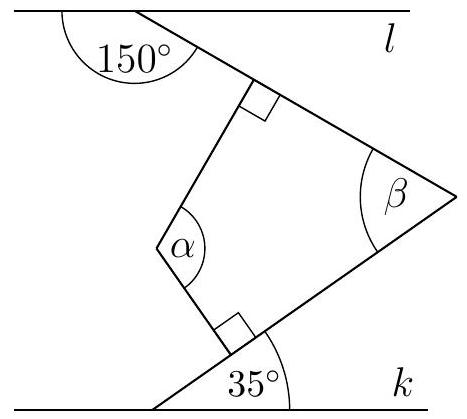
\includegraphics[max width=\textwidth, center]{2024_11_21_71f62bd117d375398909g-025}\\
32. Na rysunku obok \(k \| l\). Wyznacz \(\alpha\) i \(\beta\). Wsk. jakie proste równoległe należy dorysować?

33* W równoległoboku \(A B C D\) bok \(A B\) jest dłuższy od boku \(B C\). Dwusieczna kąta \(A D C\) przecina bok \(A B\) w punkcie \(E\). Prosta \(D E\) i prosta \(B C\) przecinając się wyznaczają dwa kąty, których miary są w stosunku \(2: 3\). Oblicz miary kątów równoległoboku \(A B C D\).

\subsection*{2.3 Twierdzenie o równoległości prostych}
Rozszerzymy obecnie, na własny użytek i tylko na użytek poniższego twierdzenia, pojęcie kątów odpowiadających nie ograniczając się wyłącznie do sytuacji z parą prostych równoległych przeciętych trzecią prostą. Otrzymamy wówczas poniższe twierdzenie, które jest twierdzeniem odwrotnym do twierdzenia o kątach naprzemianległych i odpowiadających powstałych przy przecięciu pary prostych równoległych trzecią prostą.\\
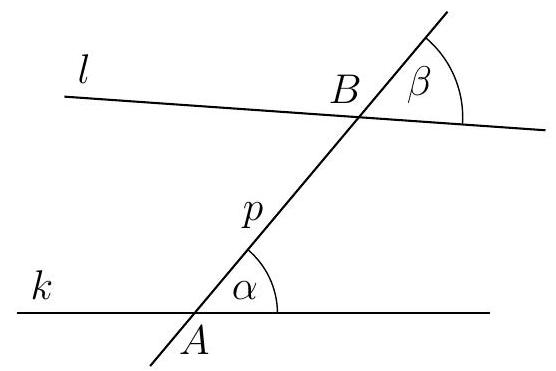
\includegraphics[max width=\textwidth, center]{2024_11_21_71f62bd117d375398909g-026}

TWIERDZENIE Niech \(k\) i \(l\) będą dwiema różnymi prostymi i niech prosta \(p\) przecina prostą \(k\) w punkcie \(A\), a prostą \(l\) w punkcie \(B\). Załóżmy ponadto, że miary odpowiadających sobie kątów \(\alpha\) i \(\beta\) są równe. Wtedy proste \(k\) i \(l\) są równoległe.\\
34. Wyznacz \(\alpha\) i \(\beta\). Rozstrzygnij czy \(\overline{A B} \| \overline{C D}\).\\
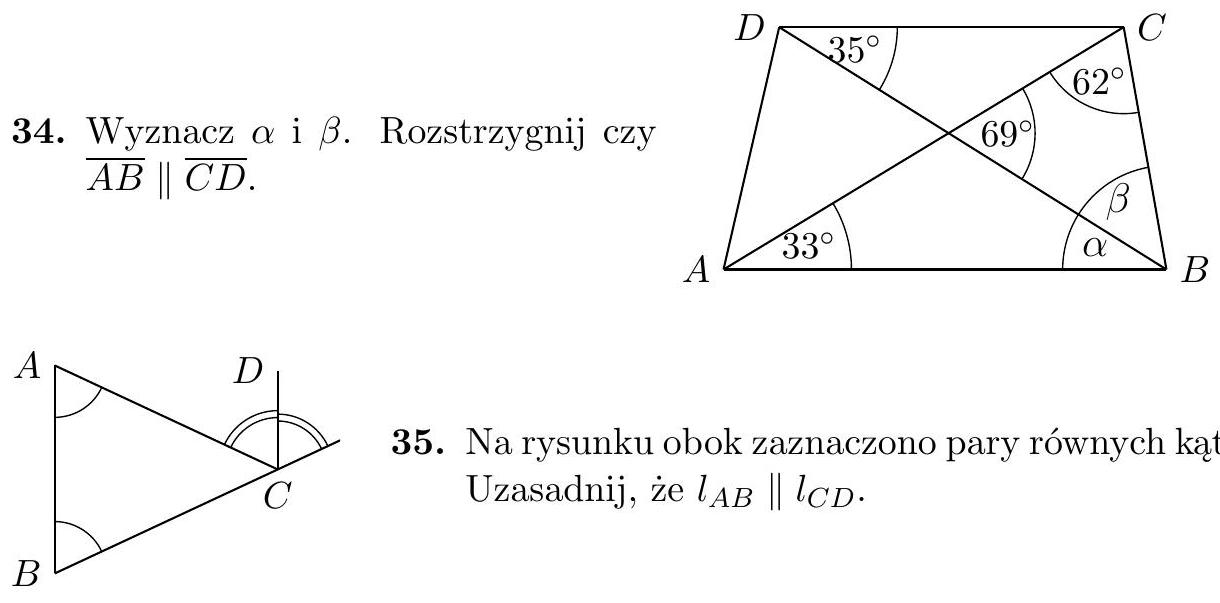
\includegraphics[max width=\textwidth, center]{2024_11_21_71f62bd117d375398909g-026(1)}\\
35. Na rysunku obok zaznaczono pary równych kątów. Uzasadnij, że \(l_{A B} \| l_{C D}\).\\
\(!\Rightarrow\) 36. W czworokącie \(A B C D\) mamy: \(\Varangle A B C=\Varangle C D A\) i \(\Varangle B C D=\Varangle B A D\). Uzasadnij, że czworokąt \(A B C D\) jest równoległobokiem.

\section*{Wskazówki i odpowiedzi.}
\begin{enumerate}
  \item \(70^{\circ}, 85^{\circ}\)
  \item \(90^{\circ}\)
  \item \(30^{\circ}, 60^{\circ}, 90^{\circ}\)
  \item \(44^{\circ}, 55^{\circ}, 81^{\circ}\)
  \item \(100^{\circ}, 60^{\circ}, 20^{\circ}\)
  \item \(\Varangle B=\alpha=30^{\circ}, \Varangle A=70^{\circ}\),\\
\(\Varangle C=80^{\circ}\)
  \item \(\Varangle A C C^{\prime}=20^{\circ}, \Varangle B C C^{\prime}=28^{\circ}\)
  \item \(\Varangle A C B=80^{\circ}\)
  \item \(\Varangle A P B=125^{\circ}\)
  \item \(135^{\circ}\)
  \item a) \(60^{\circ}\), b) \(60^{\circ}\) c) \(40^{\circ}\)\\
\(12.90^{\circ}\)
  \item wsk. przedłuż odpowiednie ramiona kątów
  \item a) \(\alpha=100^{\circ}\). b) \(\alpha=126^{\circ}\).
  \item wsk. co to jest wysokość w równoległoboku?
  \item Rozpatrz poniższe dwa przypadki\\
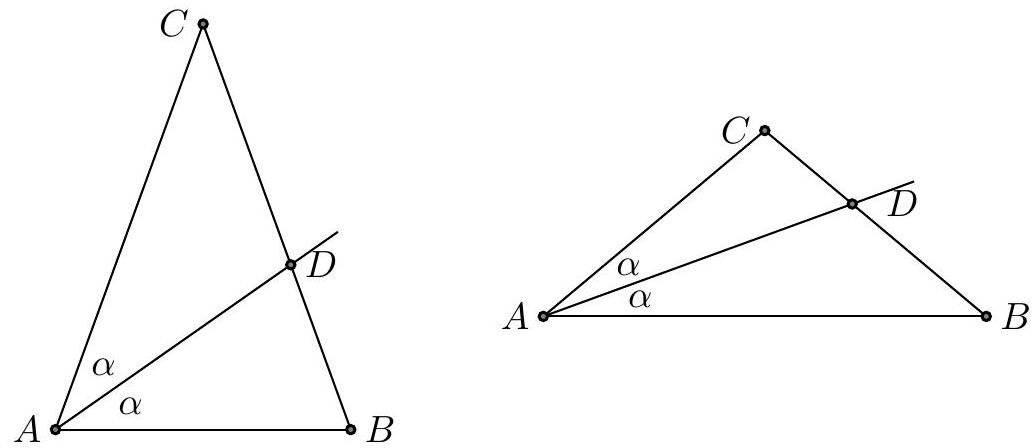
\includegraphics[max width=\textwidth, center]{2024_11_21_71f62bd117d375398909g-027(1)}
\end{enumerate}

W pierwszym przypadku mamy \(80^{\circ}, 80^{\circ}, 20^{\circ}\), a w drugim \(40^{\circ}, 40^{\circ}, 100^{\circ}\).\\
21. Spójrz na rysunek\\
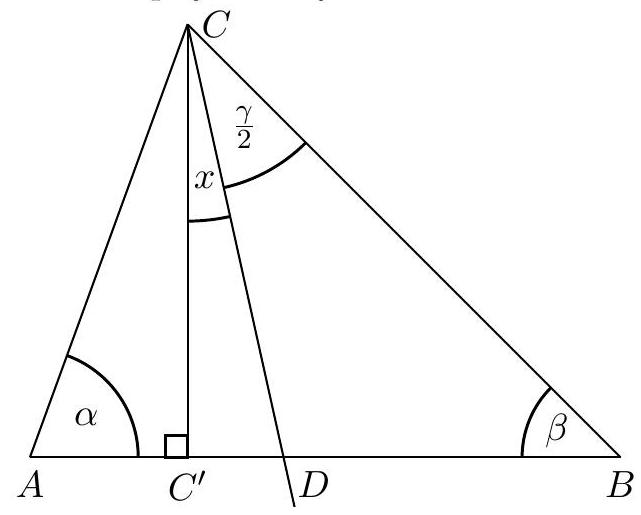
\includegraphics[max width=\textwidth, center]{2024_11_21_71f62bd117d375398909g-027}\\
i zauważ, że suma kątów ostrych w trójkącie \(A C^{\prime} C\) jest równa sumie kątów ostrych w trójkącie \(C C^{\prime} D\). To ci da równanie o zmiennej \(x\). Równie dobrze możesz skorzystać z faktu, że suma kątów ostrych w trójkącie \(A C C^{\prime}\) jest równa sumie kątów ostrych w trójkącie \(B C C^{\prime}\).\\
22. \(\alpha=25^{\circ}, \beta=83^{\circ}\)\\
23. \(60^{\circ}\)\\
25. \(40^{\circ}\) wsk. Co to jest wysokość w trójkącie?\\
26. \(36^{\circ}\)\\
27. a) \(\gamma=120^{\circ}\) b) \(\gamma=135^{\circ}\)\\
c) \(\left.\gamma=60^{\circ} \mathrm{d}\right) \gamma=30^{\circ}\) e) \(\gamma=60^{\circ}\)\\
f) \(\gamma=105^{\circ}\)\\
28. \(33^{\circ}, 57^{\circ}\)\\
29. \(82^{\circ}\)\\
30. a) \(\frac{1}{2}(\alpha+\beta)\)\\
b) \(90^{\circ}-\frac{1}{2} \alpha-\frac{1}{2} \beta\)\\
c) \(90^{\circ}+\frac{1}{2} \alpha\) d) \(\alpha+\beta\)\\
e) \(\frac{1}{2} \alpha\)\\
32. \(\alpha=115^{\circ}, \beta=65^{\circ}\)\\
33. \(108^{\circ}\) i \(72^{\circ}\)\\
34. \(\alpha=36^{\circ}, \beta=49^{\circ}\), nie są równoległe.

\section*{Rozdział 3}
\section*{POLA FIGUR.}
\begin{center}
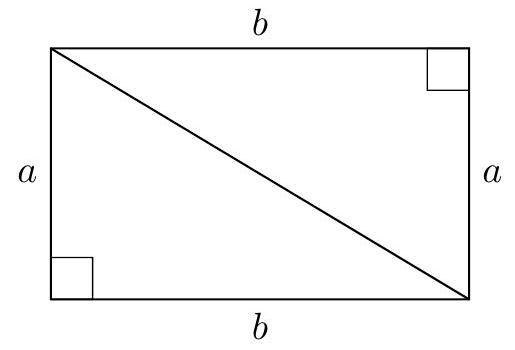
\includegraphics[max width=\textwidth]{2024_11_21_71f62bd117d375398909g-028}
\end{center}

Obecnie uporządkujemy naszą wiedzę geometryczną związaną z polem prostokąta, trójkąta, trapezu i równoległoboku. Przypomnijmy wpierw, że prostokat jest to równoległobok, w którym wszystkie kąty sa proste.

Prostokąt, w którym wszystkie boki są równej długości nazywamy kwadratem. Ponieważ prostokąt jest równoległobokiem więc jego równoległe boki są równej długości.

Teraz sformułujemy dobrze nam znany fakt geometryczny w postaci:

AKSJOMAT Pole prostokąta o bokach długości \(a, b\) równe jest \(a b\), czyli jest równe iloczynowi długości jego boków.

WNIOSEK Pole kwadratu o boku długości \(a\) jest równe \(a^{2}\).

UWAGA Przekątna prostokąta dzieli go na dwa przystające trójkąty. Z dwóch przystających trójkątów prostokątnych o przyprostokątnych \(a, b\) można „złożyć" prostokąt o bokach długości \(a, b\).

Z tego co powiedzieliśmy dotychczas wynika następujące:\\
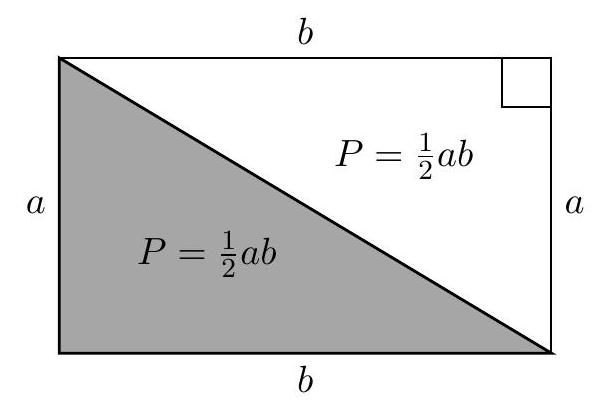
\includegraphics[max width=\textwidth, center]{2024_11_21_71f62bd117d375398909g-029(3)}

\section*{TWIERDZENIE}
Pole trójkąta prostokątnego o przyprostokątnych długości \(a\) i \(b\) jest równe połowie pola prostokąta o bokach długości \(a\) i \(b\), czyli jest równe \(\frac{1}{2} a b\) 。

W poniższych zadaniach od 1 do 4 należy korzystać tylko z wzoru na pole prostokąta oraz wzoru na pole trójkąta prostokątnego.\\
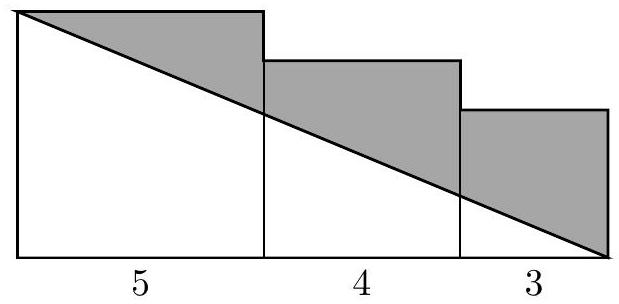
\includegraphics[max width=\textwidth, center]{2024_11_21_71f62bd117d375398909g-029}

\begin{enumerate}
  \item Figura na rysunku obok składa się z 3 kwadratów o podanych długościach boków. Wyznacz pole zacieniowanego obszaru.
  \item Figura na rysunku poniżej składa się z 4 kwadratów o podanych długościach boków. Wyznacz pole zacieniowanego obszaru.\\
\includegraphics[max width=\textwidth, center]{2024_11_21_71f62bd117d375398909g-029(2)}
  \item Figura na rysunku obok składa się z 3 kwadratów o bokach długości 6, 4, 3. Wyznacz pole zacieniowanego obszaru.\\
\includegraphics[max width=\textwidth, center]{2024_11_21_71f62bd117d375398909g-029(1)}
  \item Figura na rysunku poniżej składa się z 4 kwadratów o bokach długości \(7,8,5\) i 10. Wyznacz pole zacieniowanego obszaru.\\
\includegraphics[max width=\textwidth, center]{2024_11_21_71f62bd117d375398909g-030(2)}
\end{enumerate}

DEFINICJA Rzutem prostopadtym punktu A na prosta \(l\) jest punkt przecięcia prostej \(l\) z prostą, która przechodzi przez punkt \(A\) i jest przy tym prostopadła do \(l\).

DEFINICJA W trójkącie \(A B C\) przez \(A^{\prime}\) oznaczmy rzut prostopadły punktu \(A\) na prostą \(B C\). Wtedy odcinek \(A A^{\prime}\) nazywamy wysokościa trójkąta (wychodzącą z wierzchołka \(A\) ), zaś punkt \(A^{\prime}\) nazywamy spodkiem (podstawa) wysokości.\\
\includegraphics[max width=\textwidth, center]{2024_11_21_71f62bd117d375398909g-030(1)}

Zauważmy, że długość tego odcinka, który jest wysokością trójkąta, jest odległością wierzchołka \(A\) od prostej \(B C\), czyli krótko mówiąc \(h_{a}=d\left(A, l_{B C}\right)\). W dalszym ciągu mówiąc ogólnie o trójkącie, używać będziemy następujących oznaczeń:\\
\includegraphics[max width=\textwidth, center]{2024_11_21_71f62bd117d375398909g-030}

\begin{itemize}
  \item \(A, B, C\) - wierzchołki trójkąta
  \item \(a, b, c-\) długości boków leżących odpowiednio naprzeciwko tych wierzchołków
  \item \(\alpha, \beta, \gamma\) - odpowiednie miary kątów
  \item \(h_{a}, h_{b}, h_{c}\) - odpowiednie wysokości w trójkącie
\end{itemize}

Nazywamy je oznaczeniami standardowymi. Ich konsekwentne używanie ułatwia nam komunikację i (co za tym idzie) rozumienie (materiału). Zauważ, że na rysunku powyżej wszystkie trzy wysokości przecinają się w jednym punkcie. W rzeczywistości w każdym trójkącie ostrokątnym wysokości przecinają się w jednym punkcie. W trójkącie rozwartokątnym, trzy proste na których leżą te trzy wysokości przecinają się w jednym punkcie. Fakt ten zostanie udowodniony w dalszej części kursu. Oczywistą rzeczą jest, że wspólnym punktem wszystkich trzech wysokości trójkąta prostokątnego jest wierzchołek kąta prostego.\\
Obecnie udowodnimy twierdzenie o polu dowolnego trójkąta.

TWIERDZENIE Pole trójkąta równe jest połowie iloczynu długości boku i opuszczonej na ten bok wysokości. Czyli

\[
P=\frac{1}{2} a h_{a}=\frac{1}{2} b h_{b}=\frac{1}{2} c h_{c} .
\]

\section*{Dowód}
Wiemy już, że pole trójkąta prostokątnego równe jest \(\frac{1}{2} a h\). Pokażemy, że podobnie jest w przypadku trójkąta ostrokątnego i rozwartokątnego. Oznaczmy w obu poniższych przypadkach na użytek tego dowodu pole prostokąta, w który wpisany jest trójkąt przez \(P_{\square}\), a pole trójkąta przez \(P_{\triangle}\). Przypadek 1 - trójkąt ostrokątny.\\
\includegraphics[max width=\textwidth, center]{2024_11_21_71f62bd117d375398909g-031}

Zauważmy, że w tym przypadku wysokość \(h\) podzieliła opisany na trójkącie prostokąt na dwa prostokąty. Każdy z tych dwóch mniejszych prostokątów \(h\) podzielony jest przez odpowiedni bok trójkąta na dwa przystające trójkąty prostokątne. Wobec tego z jednej strony mamy

\[
P_{\square}=a \cdot h
\]

a z drugiej strony pole prostokąta jest sumą czterech trójkątów prostokątnych, czyli

\[
P_{\square}=P_{1}+P_{1}+P_{2}+P_{2}=2 P_{1}+2 P_{2}=2\left(P_{1}+P_{2}\right)
\]

Widać, że \(P_{\triangle}=P_{1}+P_{2}=\frac{1}{2} P_{\square}\), a ponieważ \(P_{\square}=a \cdot h\) czyli \(\frac{1}{2} P_{\square}=\frac{1}{2} a \cdot h\) więc \(P_{\triangle}=\frac{1}{2} a h\).

Przypadek 2 - trójkąt rozwartokątny.\\
\includegraphics[max width=\textwidth, center]{2024_11_21_71f62bd117d375398909g-032}\\
a ponieważ

\[
\frac{1}{2} x h=P_{x}
\]

więc wobec tego

\[
P_{\triangle}+P_{x}=\frac{1}{2} a h+P_{x}
\]

a stąd mamy

\[
P_{\triangle}=\frac{1}{2} a h .
\]

\begin{enumerate}
  \setcounter{enumi}{4}
  \item Dwa boki trójkąta sa równe 8 i 10. Wysokość poprowadzona do krótszego z nich jest równa 5. Jaką długość ma wysokość poprowadzona do drugiego boku?\\
\includegraphics[max width=\textwidth, center]{2024_11_21_71f62bd117d375398909g-032(2)}
  \item Oblicz pole trójkąta \(A C D\) na rysunku obok, jeżeli w trójkącie \(A B C\) mamy \(h_{c}=10\), w trójkącie \(A E D\) mamy \(h_{d}=5\), pola trójkątów \(A E D\) i \(B C E\) są równe, czyli krótko \(P_{A E D}=P_{B C E}\) oraz \(|E B|=4\).
  \item Na rysunku obok \(P_{A B C}=63\), \(|A D|=6,|D B|=8,|B E|=5\), \(|E C|=7\). Wyznacz \(P_{D E C}\).\\
\includegraphics[max width=\textwidth, center]{2024_11_21_71f62bd117d375398909g-032(1)}
  \item Dany jest kwadrat \(A B C D\) o polu równym 64 . Punkt \(O\) leży wewnątrz tego kwadratu, a przy tym \(P_{A B O}=6\). Wyznacz \(P_{C D O}\).
  \item Punkt \(E\) leży wewnątrz kwadratu \(A B C D\) o polu \(81 \mathrm{~cm}, P_{A B E}=15 \mathrm{~cm}^{2}\), \(P_{B C E}=12 \mathrm{~cm}^{2}\). Wyznacz wysokości trójkątów \(C D E\) i \(D A E\) wychodzące z wierzchołka \(E\).
  \item Punkt \(X\) leży wewnątrz prostokąta \(A B C D\), w którym \(|A B|=a\), \(|B C|=b\). Wyznacz \(P_{A B X}+P_{C D X}\).\\
\includegraphics[max width=\textwidth, center]{2024_11_21_71f62bd117d375398909g-033}
  \item Punkt \(X\), na rysunku obok, leży wewnątrz prostokąta \(A B C D\). Punkty \(E\) i \(F\) leżą na jego bokach, przy czym \(|A B|=7,|A D|=9,|F C|=2\), \(|E C|=3, d\left(X, l_{A B}\right)=4, d\left(X, l_{A D}\right)=1\). Wyznacz \(P_{A B X D}, P_{B D X}, P_{B E X}, P_{E C F X}, P_{B F X}\).
\end{enumerate}

\section*{PRZYKŁAD}
Stosunek długości dwóch odcinków jest równy \(2 \frac{1}{2}\). Jeden z tych odcinków jest o 8 dłuższy od drugiego. Wyznacz długości obu odcinków.

\section*{Rozwiązanie}
Oznaczmy\\
\(x\) - długość dłuższego odcinka\\
\(y\) - długość krótszego odcinka\\
Mamy wówczas

\[
\left\{\begin{array}{l}
\frac{x}{y}=2 \frac{1}{2} \\
x=y+8
\end{array}\right.
\]

Przekształcając pierwszy warunek mamy\\
\(\frac{x}{y}=\frac{5}{2}\), czyli \(5 y=2 x\), czyli \(y=\frac{2}{5} x\).\\
Wstawiając to do (2) mamy\\
\(x=\frac{2}{5} x+8\)\\
\(\frac{3}{5} x=8\)\\
\(x=\frac{40}{3}=13 \frac{1}{3}\).\\
Wstawiając to do (3) mamy\\
\(y=\frac{2}{5} \cdot \frac{40}{3}=\frac{16}{3}=5 \frac{1}{3}\).\\
Odpowiedź: długość dłuższego odcinka to \(13 \frac{1}{3}\), a krótszego \(5 \frac{1}{3}\).\\
12. Stosunek dtugości dwóch odcinków, czyli iloraz ich długości, równy jest \(1 \frac{1}{3}\). Oblicz długości tych odcinków, jeżeli jeden z nich jest o 2 dłuższy od drugiego.\\
13. Różnica długości dwóch odcinków równa jest 12, a ich stosunek długości równy jest \(2 \frac{1}{3}\). Wyznacz długości tych odcinków.\\
14. Stosunek długości dwóch odcinków równy jest 0,5 , a stosunek długości odcinków o 3 dłuższych od nich wynosi 0,6 . Wyznacz długości tych odcinków.\\
\includegraphics[max width=\textwidth, center]{2024_11_21_71f62bd117d375398909g-034(1)}\\
15. Na rysunku obok \(P_{A D C}=12 \frac{1}{2}, P_{A B C}=5\), \(|A B|=2\). Wyznacz \(|B D|\).\\
16. W czworokącie \(A B C D\) na rysunku obok przekątne \(A C\) i \(B D\) przecinają się w punkcie \(O\), przy czym \(|A O|=2,|O C|=5, P_{A O B}=3\), \(P_{C D O}=6\). Wyznacz \(P_{B C O}\) oraz wysokość \(h_{d}\) w trójkącie \(A O D\) (czyli wysokość opuszczoną na prostą \(A C)\).\\
\includegraphics[max width=\textwidth, center]{2024_11_21_71f62bd117d375398909g-034(3)}

Zauważmy teraz, że ma miejsce następujące:

\section*{TWIERDZENIE}
Jeżeli dwa trójkąty mają podstawy leżące na jednej prostej i wspólny wierzchołek poza tą prostą, to stosunek pól tych trójkątów równy jest stosunkowi długości tych podstaw.\\
\includegraphics[max width=\textwidth, center]{2024_11_21_71f62bd117d375398909g-034}

Dowód: Dla dowodu spójrz na rysunek i zauważ przy tym, że

\[
P_{A B E}=\frac{1}{2} a h, P_{C D E}=\frac{1}{2} b h, \quad \text { stąd } \quad \frac{P_{A B E}}{P_{C D E}}=\frac{\frac{1}{2} a h}{\frac{1}{2} b h}=\frac{a}{b} .
\]

\includegraphics[max width=\textwidth, center]{2024_11_21_71f62bd117d375398909g-034(2)}\\
17. Podstawy \(A B\) i \(C D\) trójkątów \(A B E\) i \(C D E\) na rysunku obok leżą na jednej prostej, przy czym \(|A B|=5,|C D|=3\), \(P_{C D E}=2\). Wyznacz \(P_{A B E}\)\\
18. Wierzchołki \(P, Q, R, S\) trójkątów \(P Q T\) i \(R S T\) leżą na jednej prostej, przy czym \(|P Q|=6,|R S|=7, P_{P Q T}=9 . \mathrm{Wy-}\) znacz \(P_{R S T}\).\\
\includegraphics[max width=\textwidth, center]{2024_11_21_71f62bd117d375398909g-035(3)}\\
19. W trójkącie \(A B C\) punkt \(D\) leży na boku \(A B\), przy czym \(|A D|=4\), \(|D B|=5, P_{A B C}=40\). Wyznacz wysokość \(h_{c}\) trójkąta \(D B C\), wychodzącą z wierzchołka \(C\).\\
\includegraphics[max width=\textwidth, center]{2024_11_21_71f62bd117d375398909g-035}\\
20. Punkty \(A, B, C, D\), na rysunku obok, leżą na jednej prostej, przy czym \(|A B|=2\), \(|B C|=3,|C D|=5, P_{C D E}=8\). Wyznacz \(P_{A B E}, P_{B C E}\).\\
21. Na przekątnej \(A C\) czworokąta \(A B C D\) obrano punkt \(E\) tak, że \(P_{A B E}=6\), \(P_{B C E}=7, P_{A D E}=5\). Wyznacz a) \(\frac{A E}{E C}\), b) \(P_{C D E}\).\\
\includegraphics[max width=\textwidth, center]{2024_11_21_71f62bd117d375398909g-035(1)}\\
22. Punkty \(A, B, D, E\) leżą na jednej prostej. Wiedząc, że \(P_{A B C}=4, P_{D E C}=14\), \(P_{D E F}=6\), wyznacz\\
a) \(\frac{A B}{D E}\),\\
b) \(P_{A B F}\).\\
\includegraphics[max width=\textwidth, center]{2024_11_21_71f62bd117d375398909g-035(2)}\\
23. Na bokach prostokąta \(A B C D\) zbudowano trójkąty \(D N E, M C E\) oraz \(A K F\) i \(L B F\), przy \(\operatorname{czym} \overline{K N} \perp \overline{A B}, \overline{L M} \perp \overline{A B}\). Wiedząc, że \(P_{M C E}=4, P_{D N E}=7\), \(P_{A K F}=3\), wyznacz \(P_{B L F}\). Wiedzacc dodatkowo, że \(|M C|=3\) wyznacz \(|D N|\) oraz wysokość \(h_{f}\) trójkąta \(K L F\) wychodzącą z wierzchołka \(F\).\\
24. Czworokąt \(A B C D\) na rysunku obok przekątne \(A C\) i \(B D\) podzieliły na cztery trójkąty. Na podstawie podanych pól trzech trójkątów wyznacz pole \(x\) czwartego trójkąta.\\
\includegraphics[max width=\textwidth, center]{2024_11_21_71f62bd117d375398909g-036}\\
25. Na poniższych trzech rysunkach trójkąt \(A B C\) został podzielony trzema odcinkami na pięć trójkątów. Na podstawie informacji o polach trzech trójkątów, wyznacz pola pozostałych dwóch trójkątów.\\
\includegraphics[max width=\textwidth, center]{2024_11_21_71f62bd117d375398909g-036(2)}\\
26. Trójkąt na rysunku obok został podzielony trzema odcinkami na pięć trójkątów. Pola dwóch z tych pięciu trójkątów są takie same. Na podstawie informacji o polach dwóch trójkątów wyznacz pola pozostałych trójkątów.

DEFINICJA Trapezem nazywamy czworokąt wypukły o co najmniej jednej parze boków równoległych. Te dwa równoległe boki nazywamy podstawami trapezu. Pozostałe dwa boki nazywamy ramionami trapezu. Odcinek prostopadły do obu podstaw łączący te podstawy, względnie proste zawierające podstawy, nazywamy wysokościa trapezu. Trapez, w którym co najmniej jeden kąt jest prosty, nazywamy trapezem prostokatnym.\\
UWAGA Z tej definicji wynika, że równoległobok jest trapezem.\\
TWIERDZENIE Pole trapezu o podstawach długości \(a, b\) oraz wysokości \(h\) równe jest \(\frac{(a+b) h}{2}\)\\
\includegraphics[max width=\textwidth, center]{2024_11_21_71f62bd117d375398909g-036(1)}

Dowód Zauważ, że w każdym z powyższych trzech przypadków przekątna trapezu dzieli go na dwa trójkąty o równoległych podstawach. A zatem wysokości obu trójkątów opuszczone na te równoległe podstawy są tej samej długości. Przeto w każdym przypadku mamy:

\[
P=\frac{1}{2} a h+\frac{1}{2} b h .
\]

Wyłączając \(\frac{1}{2} h\) przed nawias mamy:

\[
P=\frac{1}{2} h(a+b)=\frac{(a+b) h}{2} .
\]

WNIOSEK Ponieważ równoległobok jest trapezem, wobec tego pole równoległoboku jest równe iloczynowi długości boku i wysokości opuszczonej na ten bok, bo obie podstawy są w nim równej długości. Mamy zatem

\[
P=\frac{1}{2}(a+a) h=\frac{1}{2} \cdot 2 a h=a h
\]

\includegraphics[max width=\textwidth, center]{2024_11_21_71f62bd117d375398909g-037}\\
27. W kwadracie \(A B C D\) na rysunku obok długość boku jest równa 4. Punkty \(D, C, E, F\) leżą na jednej prostej. Wyznacz pole równoległoboku \(A B E F\)\\
28. Pole równoległoboku \(A B E F\) na rysunku obok równe jest 25. Wyznacz długość boku \(x\) kwadratu \(A B C D\).\\
\includegraphics[max width=\textwidth, center]{2024_11_21_71f62bd117d375398909g-037(1)}\\
29. Pole równoległoboku \(A B C D\) równe jest 100. Wyznacz pole kwadratu ABEF\\
30. W trapezie o podstawach \(b\) i \(c\) oraz wysokości \(h\) podstawa \(c\) jest trzy razy dłuższa niż \(b\), a wysokość \(h\) jest równa połowie długości \(c\). Oblicz \(b, c\) i \(h\) wiedząc, że pole trapezu równe jest polu prostokąta o bokach długości 3 i 36 .\\
31. Pole trapezu \(A B C D\) równe jest \(900 \mathrm{~cm}^{2}\). Długości podstaw trapezu równe są \(|A B|=25 \mathrm{~cm},|C D|=20 \mathrm{~cm}\). Wyznacz \(P_{A B C}\).\\
32. Punkt \(E\), na rysunku obok, leży wewnątrz trapezu prostokątnego \(A B C D\), przy czym \(|A B|=18,|C D|=10,|A D|=9\), \(d\left(E, l_{A B}\right)=2, d\left(E, l_{A D}\right)=6\). Wyznacz \(P_{B C E}, P_{A E C}\).\\
\includegraphics[max width=\textwidth, center]{2024_11_21_71f62bd117d375398909g-038(2)}\\
33. Punkt \(G\), na rysunku obok, leży wewnątrz prostokąta \(A B C D\), zaś punkty \(E\) i \(F\) leżą na jego bokach. Na podstawie podanych długości niektórych odcinków wyznacz \(P_{F G E}\), \(P_{B E F}, P_{B C E G}, P_{B D G}\).\\
34. W trapezie \(A B C D\), na rysunku obok, \(|D C|=6,|A B|=18\), wysokość \(h_{e}\) trójkąta \(C D E\) równa jest 4. Oblicz \(P_{B C E}\), jeżeli \(P_{A B C D}=84\).\\
\includegraphics[max width=\textwidth, center]{2024_11_21_71f62bd117d375398909g-038(1)}\\
35. W trapezie prostokątnym \(A B C D\), na rysunku\\
\includegraphics[max width=\textwidth, center]{2024_11_21_71f62bd117d375398909g-038}\\
obok, wysokość \(\overline{B E}\) wychodząca z wierzchołka kąta rozwartego \(\Varangle B\), ma długość 5. Podzieliła ona dłuższą podstawę trapezu na odcinki o długościach \(x\) oraz \(x+4\). Pole \(P_{A B E D}\) jest trzy razy większe od pola \(P_{B C E}\). Wyznacz długości podstaw trapezu.\\
36. Na poniższym rysunku w prostokącie \(A B C D\) punkt \(E\) leży na boku \(A B\), zaś punkt \(F\) na boku \(A D\). Wiedząc, że\\
\includegraphics[max width=\textwidth, center]{2024_11_21_71f62bd117d375398909g-039}\\
(a) \(|B C|=6,|A B|=10,|D F|=4, P_{A E F}=9\). Wyznacz \(|E B|\).\\
(b) \(|C D|=8,|B C|=5,|A E|=6, P_{C D F}\) jest o 6 większe od \(P_{A E F}\). Wyznacz \(P_{C E F}\).\\
(c) \(|A F|=2,|C D|=10,|B C|=6, P_{E B C}\) jest o 10 większe od \(P_{A E F}\). Wyznacz \(P_{F E C}\).\\
(d) \(|A B|=10,|B C|=7,|D F|=3, P_{C E F}=\) \(P_{A F E}+P_{F C D}+P_{B C E}-5\). Wyznacz \(P_{A F E}\).\\
(e) \(|A B|=10,|B C|=7,|D F|=2, P_{B C E}=3\). \(P_{F A E}\). Wyznacz \(|A E|\).\\
37. W prostokącie \(A B C D\) bok \(A B\) jest dwa razy dłuższy od boku \(B C\). Na bokach prostokata obrano punkty \(P, Q, R, S\), przy czym \(P \in \overline{A B}\) (co oznacza, że punkt \(P\) leży na boku \(A B), Q \in \overline{B C}, R \in \overline{C D}\) i \(S \in \overline{D A}\). Dane są również pewne odległości, a mianowicie: \(|A P|=6,|B P|=4\), \(|C Q|=1,|D R|=4,|A S|=3\). Wyznacz \(P_{P Q R S}\).\\
38. W prostokącie \(A B C D\) na rysunku obok mamy: \(|A B|=10,|A F|=4\), \(|A E|=2, P_{A B C D}=50, P_{E F G}=13\). Wyznacz \(|C G|\).\\
\includegraphics[max width=\textwidth, center]{2024_11_21_71f62bd117d375398909g-039(1)}\\
40. Dany jest trapez \(A B C D\) o podstawach różnej długości \(|A B|=a,|C D|=b\) i wysokości \(h\). Na odcinku będącym wysokością trapezu obieramy punkt \(E\) tak, aby \(P_{A B E}+P_{C D E}\) było równe połowie pola trapezu. Policz na jakiej długości odcinki punkt \(E\) dzieli wysokość \(h\).\\
\includegraphics[max width=\textwidth, center]{2024_11_21_71f62bd117d375398909g-040(1)}\\
41. W trapezie \(A B C D\) na rysunku obok \(P_{A B E}=33, P_{C D E}=6\). W trójkącie \(A B E\) wysokość \(h_{e}\) wychodząca z wierzchołka \(E\) ma długość 6, zaś suma (różnych) długości podstaw trapezu jest równa 17. Wyznacz wysokość \(h\) trapezu \(A B C D\) oraz \(P_{A D E}\).\\
42. W prostokątnym układzie współrzędnych zaznacz kreską odcinek \(A B, \mathrm{w}\) którym \(A=(-1,2), B=(2,2)\). Następnie zaznacz\\
(a) trzy takie punkty \(C\) leżące na jednej prostej, dla których \(P_{A B C}=3\),\\
(b) pięć takich punktów \(C\) nie leżących na jednej prostej, dla których \(P_{A B C}=3\),\\
(c) zbiór tych wszystkich punktów \(C\), dla których \(P_{A B C}=3\).

Obecnie sformułujemy kolejne twierdzenie o polach trójkątów.

TWIERDZENIE Jeżeli dwa trójkąty mają wspólną podstawę, a pozostałe wierzchołki leżą na prostej równoległej do tej podstawy, to trójkąty te mają równe pola.\\
Dowód:\\
\includegraphics[max width=\textwidth, center]{2024_11_21_71f62bd117d375398909g-040}

Rozpatrzmy trójkąty \(A B C_{1}\) i \(A B C_{2}\) o wspólnej podstawie \(A B\), przy czym \(\overline{C_{1} C_{2}} \| \overline{A B}\). Zauważmy, że wobec tego wysokości \(C_{1} C_{1}^{\prime}\) i \(C_{2} C_{2}^{\prime}\) opuszczone na prostą \(A B\) mają taką samą długość, którą oznaczmy \(h\), zaś długość podstawy \(A B\) oznaczmy \(a\). Wobec tego mamy \(P_{A B C_{1}}=\frac{1}{2} a h\), jak również \(P_{A B C_{2}}=\frac{1}{2} a h\).\\
\(!\Rightarrow\) 43. Niech dany będzie trapez \(A B C D\) o podstawach \(A B\) i \(C D\). Niech jego przekątne przecinają się w punkcie \(O\). Uzasadnij, że \(P_{B C O}=P_{D A O}\).\\
\includegraphics[max width=\textwidth, center]{2024_11_21_71f62bd117d375398909g-041(1)}\\
45. Przekątne \(A C\) i \(B D\) trapezu \(A B C D\) o podstawach \(A B\) i \(C D\) przecinają się w punkcie \(O\) i podzieliły trapez na cztery trójkąty, przy czym\\
a) \(P_{A B O}=12, P_{B C O}=7\);\\
b) \(P_{A B O}=16, P_{C D O}=9\). Wyznacz pole trapezu.\\
46. W trapezie \(A B C D\) o podstawach \(A B\) i \(C D\) przekątne \(A C\) i \(B D\) przecinają się w punkcie \(O\), przy czym \(|A B|=3, P_{A B O}=3, P_{A O D}=12\). Wyznacz\\
(a) \(P_{A B C}\),\\
(b) wysokość \(h_{c}\) w trójkącie \(A B C\),\\
(c) \(P_{C D O}\),\\
(d) wysokość \(h_{o}\) w trójkącie \(C O D\).\\
47. W trapezie \(A B C D\) o podstawach \(A B\) i \(C D\) przekątne \(A C\) i \(B D\) przecinają się w punkcie \(O\), przy czym \(P_{B C O}=3 \cdot P_{A B O},|A B|=2\). Wysokość trapezu jest równa 4. Wyznacz \(P_{A B O},|C D|\) oraz wysokość \(h_{o}\) trójkąta \(C D O\) opuszczoną na podstawę \(C D\). Wsk. w trójkątach \(A B O\) i \(C B O\) podstawy \(A O\) i \(C O\) leżą na jednej prostej, a wierzchołek \(B\) jest wspólny dla obu trójkątów. Podobnie rzecz się ma w trójkątach \(A O D\) i \(O C D\).\\
48. Na rysunku obok \(k \| l\). Wyznacz pole czworokąta \(B H E G\) wiedząc, że \(P_{A G D}=7\), zaś \(P_{C F H}=9\).\\
\includegraphics[max width=\textwidth, center]{2024_11_21_71f62bd117d375398909g-041}\\
49. Pole prostokąta jest równe polu pewnego kwadratu. Długość jednego z boków prostokąta jest o 20 większa od długości boku tego kwadratu, zaś długość drugiego boku prostokąta jest o 10 mniejsza od długości boku kwadratu. Wyznacz długość \(x\) boku kwadratu.\\
50. Kwadrat i trójkąt mają takie samo pole. Bok kwadratu i podstawa trójkąta mają taką samą długość. Wysokość trójkąta opuszczona na tę podstawę jest równa 12. Wyznacz pole trójkąta.\\
51. Uzasadnij, że jeżeli z punktu położonego wewnątrz trójkąta równobocznego poprowadzimy odcinki prostopadłe do boków trójkąta, to suma długości tych odcinków jest równa wysokości trójkąta równobocznego.\\
\includegraphics[max width=\textwidth, center]{2024_11_21_71f62bd117d375398909g-042}\\
54. Pole równoległoboku \(A B D E\) jest 3 razy mniejsze od pola prostokąta \(A C D G\). Pole kwadratu \(A B F G\) równe jest 16. Wyznacz \(|A C|\).

55* Punkt \(E\) leży na zewnątrz kwadratu \(A B C D\). Długość boku kwadratu jest równa \(a\). Oblicz pole zacieniowanego obszaru.\\
\includegraphics[max width=\textwidth, center]{2024_11_21_71f62bd117d375398909g-042(1)}

56* Pole kwadratu \(A B C D\) jest równe \(c\). Punkt \(O\) leży wewnątrz kwadratu, a przy tym \(P_{A B O}=a, P_{B C O}=b\). Wyznacz: a) \(P_{C D O}\), b) pole \(P\) prostokąta, w którym \(B O\) jest przekątną, a pozostałe dwa wierzchołki leżą na bokach \(A B\) i \(B C\) kwadratu \(A B C D\).

57* W trójkącie \(A B C\) kąt przy wierzchołku \(C\) jest prosty, \(|B C|=15\), \(|A C|=20,|A B|=25\). Punkt \(D\) leży na boku \(A B\) i jest tak samo oddalony od prostej \(A C\) jak od prostej \(B C\). Wyznacz tę odległość \(d\).

58* W trapezie \(A B C D\) o podstawach \(A B\) i \(C D:|A B|=a,|C D|=b\), wysokość ma długość \(h\). Punkt \(E\) leży wewnątrz trapezu. Wyznacz odległość \(d\) punktu \(E\) od podstawy \(A B\) tak, aby \(P_{A B E}+P_{C D E}=P_{B C E}+P_{A D E}\).\\
59. W trójkącie prostokątnym \(A B C\) kąt \(C\) jest prosty, \(|A C|=6,|B C|=8\). Dwusieczna kata prostego przecina bok \(A B\) w punkcie \(D\). Wyznacz \(P_{A D C}\) i \(P_{D C B}\).\\
60. Na rysunku obok punkty \(P, Q, R, S\) są środkami boków czworokąta \(A B C D\). Uzasadnij, że zacieniowane pole jest połową pola czworokąta \(A B C D\).\\
\includegraphics[max width=\textwidth, center]{2024_11_21_71f62bd117d375398909g-043}\\
61. Trójkąt \(A B C\) na rysunku obok ma pole równe 7. Odcinek \(A B^{\prime}\) jest dwukrotnie dłuższy od odcinka \(A B\), zaś odcinek \(C A^{\prime}\) jest dwukrotnie dłuższy od odcinka \(C A\). Wyznacz pole trójkąta \(A B^{\prime} C\) oraz trójkąta \(A^{\prime} B^{\prime} C\) 。

\section*{Wskazówki i odpowiedzi.}
\begin{enumerate}
  \item \(P=20\)
  \item \(P=83 \frac{1}{2}\)
  \item \(P=42\)
  \item \(P=92\)
  \item \(h=4\)
  \item \(P_{A C D}=20\)
  \item \(P_{D E C}=21\)
  \item \(P_{C D O}=26\)
  \item w trójkącie \(C D E \quad h=5 \frac{2}{3}\), w trójkącie \(D A E h=6 \frac{1}{3}\)
  \item \(P_{A B X}+P_{C D X}=\frac{1}{2} a b\)
  \item \(P_{A B X D}=18 \frac{1}{2}, \quad P_{B D X}=13\),\\
\(P_{B E X}=18, P_{E C F X}=14\),\\
\(P_{B F X}=23\)
  \item 6 i 8
  \item 21 i 9\\
14.6 i 12
  \item \(|B D|=3\)
  \item \(P_{B C O}=7 \frac{1}{2}, h=2 \frac{2}{5}\)
  \item \(P_{A B E}=3 \frac{1}{3}\)
  \item \(P_{R S T}=10 \frac{1}{2}\)
  \item \(h_{c}=8 \frac{8}{9}\)
  \item \(P_{B C E}=4 \frac{4}{5}, P_{A B E}=3 \frac{1}{5}\)
  \item \(\frac{A E}{E C}=\frac{6}{7}, P_{C D E}=5 \frac{5}{6}\)
  \item \(\frac{A B}{D E}=\frac{2}{7}, P_{A B F}=\frac{12}{7}\)
  \item \(P_{B L F}=1 \frac{5}{7}, D N=5 \frac{1}{4}, h_{f}=1 \frac{1}{7}\)
  \item \(3 \frac{3}{5}\)
  \item a) \(x=4, y=9 \frac{1}{3}\), b) \(x=4, y=3\),\\
c) \(x=2, y=5\)
  \item \(x=6, y=9\)
  \item \(P_{A B E F}=16\)
  \item \(x=5\)
  \item \(P_{A B E F}=100\)
  \item \(b=6, c=18, h=9\)
  \item \(P_{A B C}=500 \mathrm{~cm}^{2}\)
  \item Wsk. Wpierw zrób staranny rysunek, a nasteqpnie wyznacz kolejno\\
\(P_{F E C D}, P_{G B E}\), itd.\\
odp. \(P_{B C E}=46, P_{A E C}=17\)
  \item \(P_{F G E}=10, P_{B E F}=34\), \(P_{B C E G}=34, P_{B D G}=9\)
  \item \(P_{B C E}=45\)
  \item a) \(|E B|=1\), b) \(P_{C E F}=17\),\\
c) \(P_{F E C}=20\),\\
d) \(P_{A F E}=16 \frac{2}{3}\),\\
e) \(|A E|=3 \frac{3}{11}\)
  \item \(P_{P Q R S}=26\)
  \item \(|A B|=12,|C D|=20\)
  \item \(|C G|=3\)
  \item \(P_{A B C D}=66, P_{B C E}=23\)
  \item Odcinki równej długości czyli \(\frac{h}{2}\)
  \item \(h=8, P_{A D E}=29\)
  \item wsk.skorzystaj z odpowiedniego twierdzenia o polach trójkątów 44. \(P_{A B O}=90\)
  \item a) \(P_{A B C D}=30 \frac{1}{12}\),\\
b) \(P_{A B C D}=49\)
  \item \(P_{A B C}=15, h_{c}=10\),\\
\(P_{C D O}=48, h_{o}=8\)
  \item \(P_{A B O}=1, C D=6, h_{o}=3\)
  \item \(P_{B H E G}=16\)
  \item \(x=20\)
  \item \(P=36\)
  \item wsk. zauważ, że ten punkt dzieli nasz trójkąt równoboczny na trzy trójkąty
  \item \(|A C|=12\)
  \item \(\frac{1}{2} a^{2}\)
  \item \(P_{C D O}=\frac{1}{2} c-a, P=\frac{4 a b}{c}\)
  \item \(d=8 \frac{4}{7}\)
  \item \(d=\frac{1}{2} h\)
  \item \(P_{A D C}=10 \frac{2}{7}, P_{B C D}=13 \frac{5}{7}\)
  \item \(P_{A B^{\prime} C}=14, P_{A^{\prime} B^{\prime} C}=28\)
\end{enumerate}

\section*{Rozdział 4}
\section*{TRÓJKĄTY PRZYSTAJĄCE.}
\begin{center}
\includegraphics[max width=\textwidth]{2024_11_21_71f62bd117d375398909g-045(1)}
\end{center}

DEFINICJA Dwa trójkąty nazywamy przystającymi, jeżeli mają odpowiadające sobie boki i odpowiadające sobie kąty równe.

To, że trójkąt \(A B C\) przystaje do trójkąta \(A^{\prime} B^{\prime} C^{\prime}\) będziemy oznaczać \(\triangle A B C \equiv \triangle A^{\prime} B^{\prime} C^{\prime}\).

Zapis \(\triangle A B C \equiv \triangle A^{\prime} B^{\prime} C^{\prime}\) oznacza, że

\[
|A B|=\left|A^{\prime} B^{\prime}\right|,|B C|=\left|B^{\prime} C^{\prime}\right|,|A C|=\left|A^{\prime} C^{\prime}\right|
\]

oraz

\[
\Varangle A B C=\Varangle A^{\prime} B^{\prime} C^{\prime}, \Varangle B C A=\Varangle B^{\prime} C^{\prime} A^{\prime}, \Varangle C A B=\Varangle C^{\prime} A^{\prime} B^{\prime}
\]

Faktycznie, na to aby stwierdzić czy dwa dane trójkąty są przystające, nie potrzeba sprawdzać czy wszystkie odpowiadające sobie boki i kąty są równe. Rozstrzygają bowiem o tym tzw. cechy przystawania trójkatów.

Cecha BBB (bok, bok, bok)\\
Jeżeli w trójkątach \(A B C\) i \(A^{\prime} B^{\prime} C^{\prime}\) zachodzą równości:\\
\(|A B|=\left|A^{\prime} B^{\prime}\right|\),\\
\(|B C|=\left|B^{\prime} C^{\prime}\right|\),\\
\(|A C|=\left|A^{\prime} C^{\prime}\right|\),\\
to te trójkąty są przystające, a dokładniej to \(\triangle A B C \equiv \triangle A^{\prime} B^{\prime} C^{\prime}\).\\
Oznacza to, że dwa trójkąty przystają do siebie, jeżeli odpowiadające sobie boki mają równe\\
\includegraphics[max width=\textwidth, center]{2024_11_21_71f62bd117d375398909g-045}\\
długości.

\section*{PRZYKŁAD}
Dany jest czworokąt \(A B C D\), w którym \(|A B|=|C D|\) oraz \(|A D|=|B C|\). Uzasadnij, że \(\triangle A D B \equiv \triangle C B D\).

\section*{Uzasadnienie}
W trójkątach \(A B D\) i \(C D B\) z założenia mamy:

\[
\begin{aligned}
& |A B|=|C D| \\
& |A D|=|B C|
\end{aligned}
\]

Odcinek \(B D\) jest wspólny dla obu trójkątów. Wobec tego na mocy cechy BBB przystawania trójkątów \(\triangle A D B \equiv \triangle C B D\).\\
Podobnie uzasadniamy, że \(\triangle A B C \equiv \triangle C D A\).\\
\includegraphics[max width=\textwidth, center]{2024_11_21_71f62bd117d375398909g-046(2)}

Cecha BKB (bok, kąt, bok):\\
Jeżeli dla trójkątów \(A B C\) i \(A^{\prime} B^{\prime} C^{\prime}\) zachodzą równości:\\
\(|B A|=\left|B^{\prime} A^{\prime}\right|\),\\
\(\Varangle B A C=\Varangle B^{\prime} A^{\prime} C^{\prime}\),\\
\(|A C|=\left|A^{\prime} C^{\prime}\right|\),\\
to \(\triangle A B C \equiv \triangle A^{\prime} B^{\prime} C^{\prime}\).\\
Oznacza to, że jeżeli w jednym trójkącie długości dwóch boków i kąt między nimi zawarty są takie same jak długości dwóch boków i kąt między nimi zawarty w drugim trójkącie, to te trójkąty są przystające.\\
\includegraphics[max width=\textwidth, center]{2024_11_21_71f62bd117d375398909g-046}

Natomiast sama równość dwóch boków i równość jakichkolwiek kątów w dwóch trójkątach nie oznacza, że te dwa trójkąty są przystające. Weźmy bowiem, na przykład, dwa trójkąty: \(A B C\) i \(A B C^{\prime}\), w których \(|B C|=\left|B C^{\prime}\right|\), zaś \(A B\) jest wspólnym bokiem obu trójkątów (czyli te trójkąty mają po dwa boki równej długości), a przy tym \(\Varangle C A B=\Varangle C^{\prime} A B=30^{\circ}\), na-\\
\includegraphics[max width=\textwidth, center]{2024_11_21_71f62bd117d375398909g-046(1)}\\
tomiast trójkąty te nie są przystające.

\section*{PRZYKŁAD}
Przekątna \(B D\) podzieliła czworokąt \(A B C D\) na dwa trójkąty, przy czym \(|A B|=|C D|\) oraz \(\Varangle A B D=\Varangle C D B\). Uzasadnij, że \(\triangle A B D \equiv \triangle C D B\).

\section*{Uzasadnienie}
W trójkątach \(A B D\) i \(C B D\) z założenia mamy:

\[
\begin{aligned}
& |A B|=|C D|, \\
& \Varangle A B D=\Varangle C D B .
\end{aligned}
\]

Odcinek \(B D\) jest wspólny dla obu trójkątów. Wobec tego na mocy cechy BKB przystawania trójkątów \(\triangle A B D \equiv \triangle C D B\).\\
\includegraphics[max width=\textwidth, center]{2024_11_21_71f62bd117d375398909g-047(1)}

Cecha KBK (kąt, bok, kąt):\\
Jeżeli dla trójkątów \(A B C\) i \(A^{\prime} B^{\prime} C^{\prime}\) zachodzą równości\\
\(|A B|=\left|A^{\prime} B^{\prime}\right|\),\\
\(\Varangle B A C=\Varangle B^{\prime} A^{\prime} C^{\prime}\),\\
\(\Varangle A B C=\Varangle A^{\prime} B^{\prime} C^{\prime}\),\\
to te trójkąty są przystające.\\
Innymi słowy, jeżeli w jednym i drugim trójkącie dany jest bok o takiej samej długości i przyległe do tych boków kąty w obu trójkątach mają takie\\
\includegraphics[max width=\textwidth, center]{2024_11_21_71f62bd117d375398909g-047(2)}\\
same miary, to te trójkąty są przystające.\\
Natomiast sama równość dwóch kątów i równość jakichkolwiek boków w tych dwóch trójkątach nie oznacza, że te dwa trójkąty są przystające. Weźmy, na przykład, trójkąt prostokątny \(A B C\), w którym \(\Varangle C A B=30^{\circ}, \Varangle A C B=\) \(90^{\circ}, \Varangle A B C=60^{\circ}\), zaś \(|B C|=5\). Wysokość \(C D\) dzieli ten trójkąt na dwa trójkąty. Widać, że w trójkątach \(B C D\) i \(A B C\) są takie same kąty oraz, że jeden bok, a mianowicie \(B C\), jest wspólny dla obu trójkątów. Trójkąty te jednak nie są przystające, bowiem kąty przy boku \(B C\) w obu trójkątach nie są takie same.\\
\includegraphics[max width=\textwidth, center]{2024_11_21_71f62bd117d375398909g-047}

\section*{PRZYKŁAD}
Odcinek \(B D\) podzielił czworokąt \(A B C D\) na dwa trójkąty, przy czym \(\Varangle A B D=\Varangle C B D\) oraz \(\Varangle A D B=\Varangle C D B\). Pokaż, że \(\triangle A B D \equiv \triangle C B D\).

\section*{Uzasadnienie}
W trójkątach \(A B D\) i \(C D B\) z założenia mamy:

\[
\begin{aligned}
& \Varangle A D B=\Varangle C D B, \\
& \Varangle A B D=\Varangle C B D .
\end{aligned}
\]

Odcinek \(B D\) jest wspólny dla obu trójkątów.\\
Wobec tego, na mocy cechy KBK przystawania trójkątów, \(\triangle A B D \equiv \triangle C B D\).\\
\includegraphics[max width=\textwidth, center]{2024_11_21_71f62bd117d375398909g-048(1)}

W poniższych zadaniach tam, gdzie nie ma rysunku sporządź rysunek. Uzasadnienia rób takim językiem jak w podanych powyżej przykładach.\\
Większość uzasadnień jest na końcu rozdziału.

\begin{enumerate}
  \item Przekątna \(B D\) podzieliła czworokąt \(A B C D\) na dwa trójkąty, przy czym \(\Varangle A D B=\Varangle C B D\) i \(\Varangle A B D=\Varangle C D B\). Uzasadnij, że \(\triangle A B D \equiv \triangle C D B\).
  \item Odcinki \(A B\) i \(C D\) przecinają się w punkcie \(O\), przy czym \(|A O|=|O B|\) i \(|C O|=|O D|\). Uzasadnij, że \(\triangle D O B \equiv \triangle C O A\) oraz, że \(|A C|=|B D|\) oraz, że \(|A D|=|B C|\).
  \item Odcinek \(A C\) dzieli czworokąt \(A B C D\) na trójkąty \(A B C\) i \(A D C\) przy czym \(|A B|=|A D|\) oraz \(\Varangle B A C=\Varangle D A C\). Uzasadnij, że \(|B C|=|D C|\).
  \item W kwadracie \(A B C D\) o boku długości \(a\) punkt \(E\) jest środkiem boku \(B C\), punkt \(F\) jest środkiem boku \(C D\). Uzasadnij, że \(\triangle A D F \equiv \triangle A B E\).\\
\includegraphics[max width=\textwidth, center]{2024_11_21_71f62bd117d375398909g-048}
  \item Na rysunku obok \(\Varangle D A B=\Varangle C B A \mathrm{i} \Varangle C A B=\) \(\Varangle D B A\). Uzasadnij, że \(\triangle C A B \equiv \triangle D B A\).
  \item Końce odcinka \(A B\) leżą na dwóch prostych równoległych. Przez środek \(O\) tego odcinka prowadzimy dowolny odcinek \(C D\), którego końce leżą na tych samych równoległych, przy czym punkt \(C\) leży na tej prostej co punkt \(B\). Udowodnij, że \(|C O|=|O D|\).\\
\(!\Rightarrow\) 7. Uzasadnij, że w równoległoboku boki równoległe są równej długości.\\
\(!\Rightarrow\) 8. Uzasadnij, że punkt przecięcia przekątnych równoległoboku dzieli każdą z nich na połowy.
\end{enumerate}

Wyniki ostatnich dwóch zadań oraz zadanie 20 z rozdziału 1 można krótko sformułować następująco:

W równoległoboku:

\begin{itemize}
  \item kąty przeciwległe są równe,
  \item odcinki przeciwległe są równej długości,
  \item punkt przecięcia przekątnych dzieli każdą z nich na połowy.
\end{itemize}

\begin{enumerate}
  \setcounter{enumi}{8}
  \item Odcinki \(A B\) i \(C D\) przecinają się w punkcie \(O\), przy czym \(|A O|=|O B|\) i \(|C O|=|O D|\). Uzasadnij, że \(|A C|=|B D|\).
  \item Odcinki \(A D\) i \(B C\) przecinają się w punkcie \(O\), przy czym \(|B O|=|C O|\) oraz \(\Varangle A C O=\Varangle O B D\). Uzasadnij kolejno, że \(\triangle D O B \equiv \triangle A O C\) i \(\triangle B O A \equiv \triangle C O D\).
  \item Dany jest trójkąt równoramienny \(A B C\), w którym \(|A C|=|B C|\). Z wierzchołka \(C\) odłożono na bokach \(C A\) i \(C B\) równej długości odcinki, odpowiednio: \(C A_{1}\) i \(C B_{1}\). Pokaż, że \(\triangle C A B_{1} \equiv \triangle C B A_{1}\).
  \item Na boku \(A B\) trójkąta \(A B C\) obrano punkt \(D\), a na boku \(A_{1} B_{1}\) trójkąta \(A_{1} B_{1} C_{1}\) obrano punkt \(D_{1}\). Wiadomo przy tym, że \(\triangle A D C \equiv \triangle A_{1} D_{1} C_{1}\) i że \(|D B|=\left|D_{1} B_{1}\right|\). Pokaż, że \(\triangle A B C \equiv \triangle A_{1} B_{1} C_{1}\).
  \item W kwadracie \(A B C D\) punkty \(P, Q, R\) i \(S\) leżą na bokach \(A B, B C, C D\) i \(D A\) odpowiednio, w taki sposób, że \(|A P|=|B Q|=|C R|=|D S|\). Wykaż, że czworokąt \(P Q R S\) jest kwadratem.
  \item Przekątna \(B D\) podzieliła czworokąt \(A B C D\) na dwa trójkąty, przy czym \(\Varangle A D B=\Varangle C B D\) i \(\Varangle A B D=\Varangle C D B\). Uzasadnij, że \(\Varangle D C A=\Varangle B A C\).
  \item Punkty \(A, B, C, D, E\) leżą na jednej prostej tak jak na rysunku obok, zaś punkty \(F\) i \(G\) poza nią, przy \(\operatorname{czym}|B C|=|C D|,|B F|=|D G|\), \(\Varangle A B F=\Varangle E D G\). Uzasadnij, że \(\triangle B C F \equiv \triangle D C G\).\\
\includegraphics[max width=\textwidth, center]{2024_11_21_71f62bd117d375398909g-049}
  \item Punkty \(A, B, C, D\) leżą w tej właśnie kolej-\\
\includegraphics[max width=\textwidth, center]{2024_11_21_71f62bd117d375398909g-050(1)}\\
ności na jednej prostej, przy czym \(A B=C D\). Punkty \(E\) i \(F\) leżą po przeciwnych stronach tej prostej, przy czym \(\Varangle E B D=\Varangle F C A, \Varangle F A C=\Varangle E D B\). Uzasadnij kolejno, że\\
a) \(\triangle A F C \equiv \triangle D E B\),\\
b) \(\triangle A B E \equiv \triangle D C F\).
  \item Punkty \(A, C, B, D\) leżą w tej właśnie kolejności na jednej prostej, przy czym \(A B=C D\). Punkty \(E, F\) leżą po przeciwnych stronach tej prostej, przy czym \(\Varangle E B D=\Varangle F C A, \Varangle F A C=\Varangle E D B\). Uzasadnij kolejno, że\\
a) \(\triangle A F C \equiv \triangle D E B\),\\
b) \(\triangle A B E \equiv \triangle D C F\),\\
c) \(\triangle A E D \equiv \triangle D F A\).\\
\includegraphics[max width=\textwidth, center]{2024_11_21_71f62bd117d375398909g-050}
  \item Na rysunku obok \(\Varangle D A B=\Varangle C B A\) i \(\Varangle C A B=\) \(\Varangle D B A\). Uzasadnij, że \(\triangle A P C \equiv \triangle B P D\).
  \item Na rysunku obok \(|B C|=|A C|\) oraz \(\Varangle D B C=\Varangle E A C\). Uzasadnij kolejno, że\\
(a) \(\triangle A C E \equiv \triangle B C D\),\\
(b) \(\triangle B Q E \equiv \triangle A Q D\),\\
(c) \(\triangle B A E \equiv \triangle A B D\).\\
\includegraphics[max width=\textwidth, center]{2024_11_21_71f62bd117d375398909g-050(2)}
  \item Na rysunku obok \(|B D|=|D F|\) oraz \(\Varangle C B D=\Varangle E F D\). Pokaż, że \(|C F|=|B E|\).
  \item Na rysunku obok \(|A B|=|A F|\) oraz \(|A C|=|A E|\). Pokaż, że \(\Varangle A C F=\Varangle A E B\).
  \item Odcinki \(A D\) i \(B C\) przecinają się w punkcie \(O\), przy czym \(|B O|=|C O|\) oraz \(\Varangle A C O=\Varangle O B D\). Uzasadnij, że \(\triangle A B C \equiv \triangle C D B\).
  \item W sześciokącie \(K L M N O P\) na rysunku obok \(|K P|=|K L|,|P O|=|L M|\), \(|O N|=|M N|\) oraz \(\Varangle O N K=\Varangle M N K\).\\
Pokaż, że \(\Varangle K P O=\Varangle K L M\).\\
\includegraphics[max width=\textwidth, center]{2024_11_21_71f62bd117d375398909g-051}
  \item Odcinki \(A B\) i \(C D\) przecinają się w punkcie \(E\), przy czym \(|A E|=|E D|\) oraz \(\Varangle E A F=\) \(\Varangle E D G\). Uzasadnij, że \(\triangle A C E \equiv \triangle D B E\). Dorysuj następnie odcinek \(B C\). Uzasadnij, że \(\triangle A B C \equiv \triangle D C B\). A teraz dorysuj odcinek \(A D\) i uzasadnij, że uzyskałeś dwa kolejne trójkąty przystające.
  \item W czworokącie \(A B C D\) mamy \(|A B|=|C D|\) i \(|A D|=|B C|\). Uzasadnij, ! \(\Leftarrow\) że czworokąt \(A B C D\) jest równoległobokiem.
  \item W czworokącie \(A B C D\) mamy: \(|A B|=|C D|\) i \(\overline{A B} \| \overline{C D}\). Uzasadnij, że ! \(\Leftarrow\) \(A B C D\) jest równoległobokiem.
  \item Przekątne \(A C\) i \(B D\) czworokąta \(A B C D\) przecinają się w punkcie \(O\), który dzieli każdą z nich na połowy. Uzasadnij, że czworokąt \(A B C D\) jest równoległobokiem.
\end{enumerate}

Wyniki ostatnich trzech zadan i zadania 36 z rozdziału o kątach w trójkącie, można sformułować w postaci

\section*{TWIERDZENIE}
Jeżeli w czworokącie, spełniony jest jeden z warunków:

\begin{itemize}
  \item obie pary odcinków przeciwległych są równej długości,
  \item obie pary przeciwległych kątów są równej miary
  \item jedna para przeciwległych boków jest równoległa i równej długości
  \item punkt przecięcia przekątnych dzieli każdą z nich na połowy,\\
to ten czworokąt jest równoległobokiem.
\end{itemize}

\begin{enumerate}
  \setcounter{enumi}{27}
  \item Trójkąty \(A B C\) i \(P Q R\) są przystające, przy czym \(\triangle A B C \equiv \triangle P Q R\). Pokaż, że wysokość poprowadzona z wierzchołka \(C\) w trójkącie \(A B C\) jest równa wysokości poprowadzonej z wierzchołka \(R\) w trójkącie \(P Q R\).
  \item W trójkącie prostokątnym \(A B C\) kąt \(C\) jest prosty, \(|A B|=c\),\\
\(|B C|=a,|A C|=b\). Dwusieczne kątów ostrych przecinają się w punkcie \(D\). Wyznacz odległość punktu \(D\) od boków tego trójkąta. Wsk. skorzystaj z odpowiedniego zadania o przystawaniu trójkątów.\\
\includegraphics[max width=\textwidth, center]{2024_11_21_71f62bd117d375398909g-052}
  \item W prostokącie \(A B C D\), na rysunku obok, poprowadzono przekątne \(A C\) i \(B D\), które przecinają się w punkcie \(O\). Przez punkt \(O\) poprowadzono odcinki \(E F\) i \(G H\) łączące przeciwległe boki prostokąta.\\
(a) Uzasadnij, że \(\triangle O C F \equiv \triangle O A E, \triangle G O F \equiv \triangle H O E\).\\
(b) Uzasadnij, że wysokość trójkąta \(C F O\) opuszczona na prostą \(F C\) ma długość 4 , wiedząc, że długość boku \(B C\) jest równa 8.\\
(c) Wyznacz pole zacieniowanego obszaru na podstawie podanych długości odcinków.\\
\includegraphics[max width=\textwidth, center]{2024_11_21_71f62bd117d375398909g-052(1)}
  \item Punkty \(A, B, C\) na rysunku obok leżą na jednej prostej, przy czym \(|A B|=7,|A C|=12,|C D|=4\). Korzystając tylko z cech przystawania trójkątów oraz poznanych wzorów na pole trójkąta czy też trapezu wyznacz \(|A E|\).
  \item Przekątne prostokąta \(A B C D\) na rysunku obok przecinają się w punkcie \(O\). Uzasadnij, że \(P_{E C O}=P_{F A O}\).\\
\includegraphics[max width=\textwidth, center]{2024_11_21_71f62bd117d375398909g-052(2)}
  \item Wiedząc, że \(O\) jest punktem przecięcia przekątnych w prostokącie na rysunku obok korzystając z wyniku poprzedniego zadania, wyznacz pole \(P\) zacieniowanego obszaru.
  \item W równoległoboku \(A B C D\) poprowadzono przekątną \(A C\). Wykaż, że \(d\left(D, l_{A C}\right)=d\left(B, l_{A C}\right)\).
\end{enumerate}

DEFINICJA Środkowa w trójkącie nazywamy odcinek łączący środek boku trójkąta z przeciwległym mu wierzchołkiem trójkąta.\\
35. Uzasadnij, że jeżeli w trójkącie \(A B C\) boki \(A C\) i \(B C\) są równej długości, to \(\Varangle C A B=\Varangle C B A\). wsk. poprowadź środkową \(C D\).\\
36. Uzasadnij, że jeżeli w trójkącie \(A B C\) kąty \(\Varangle C A B\) i \(\Varangle C B A\) są równe, to \(|A C|=|B C|\). wsk. poprowadź dwusieczną kąta \(\Varangle A C B\).

Ostatnie dwa zadania są treścią podstawowego twierdzenia geometrii o trójkącie równoramiennym. Historyczna nazwa tego twierdzenia brzmi: Pons Asinorum - po polsku Ośli Most. Mamy zatem

\section*{TWIERDZENIE Pons Asinorum}
W trójkącie\\
(1) na przeciwko równych boków leżą równe kąty,\\
(2) na przeciwko równych kątów leżą równe boki.

W kolejnych zadaniach będziemy korzystać właśnie z tego twierdzenia.\\
DEFINICJA Trójkąt o wszystkich bokach równych nazywamy trójkatem równobocznym.\\
37. Uzasadnij, że w trójkącie równobocznym wszystkie kąty są równe.\\
38. Uzasadnij, że jeżeli w trójkącie wszystkie kąty są równe, to jest to trójkąt równoboczny.\\
39. Uzasadnij, że w trapezie równoramiennym, który nie jest równoległobo- \(\qquad\) kiem, kąty przy podstawie są równe.\\
40. Uzasadnij, że jeżeli w trapezie kąty przy podstawie są równe, to ten trapez jest równoramienny, a jego przekątne są równej długości.\\
41. W trójkącie \(A B C\) dwusieczna kąta \(A\) jest prostopadła do boku \(B C\), zaś dwusieczna kąta \(B\) jest prostopadła do boku \(A C\). Uzasadnij, że ten trójkąt ma wszystkie boki równej długości.\\
42. W trójkącie równobocznym \(A B C\) przedłużono bok \(A B\) o odcinek \(B B^{\prime}\), bok \(B C\) o odcinek \(C C^{\prime}\) i bok \(C A\) o odcinek \(A A^{\prime}\), przy czym \(\left|A A^{\prime}\right|=\) \(\left|B B^{\prime}\right|=\left|C C^{\prime}\right|=1\). Uzasadnij, że trójkąt \(A^{\prime} B^{\prime} C^{\prime}\) jest równoboczny.\\
43. W trójkącie \(A B C\) poprowadzono środkową \(A D\). Pokaż, że wierzchołki \(B\) i \(C\) są jednakowo odległe od prostej \(A D\). Rozpatrz trójkąt, w którym żadne dwa boki nie są równej długości. Wsk. co to jest odległość punktu od prostej?\\
\(!\Rightarrow 44\). Uzasadnij, że jeżeli punkt leży na dwusiecznej kąta, to jest on tak samo odległy od obu ramion kąta.\\
45. Uzasadnij, że jeżeli trójkąt jest równoramienny, to wysokości opuszczone na równe boki są równej długości. Rozpatrz zarówno trójkąt rozwartokątny jak i ostrokątny.\\
46. Uzasadnij, że jeżeli w trójkącie dwie wysokości są równej długości, to boki na które są one opuszczone są równej długości czyli ten trójkąt jest równoramienny.\\
47. Uzasadnij, że w trójkącie równoramiennym dwusieczne kątów przy podstawie są równej długości.\\
48. Uzasadnij, że w trójkącie równoramiennym środkowe wychodzące z wierzchołków przy podstawie są równej długości.\\
49. Dany jest kąt o wierzchołku \(O\). Niech półprosta \(O S\) będzie jego dwusieczną. Prowadzimy prostą prostopadłą do tej dwusiecznej. Ta prosta przecina ramiona kąta w punktach \(A\) i \(B\). Uzasadnij, że trójkąt \(A O B\) jest równoramienny.\\
\includegraphics[max width=\textwidth, center]{2024_11_21_71f62bd117d375398909g-054}\\
50. (matura 2010) Trójkąty równoramienne \(A B C\) i \(D E C\) na rysunku obok mają wspólny wierzchołek \(C\), a przy tym \(\Varangle A C B=\Varangle D C E=90^{\circ}\). Uzasadnij, że \(|A D|=B E \mid\).

Poniższe zadania są trudniejsze: wymagają pomysłu. Dobrze jest jednak zapoznać się z poniższym przykładem, a następnie rozwiązać kolejne dwa zadania opierając się na przygotowanych szkicach rozwiązań.\\
\includegraphics[max width=\textwidth, center]{2024_11_21_71f62bd117d375398909g-055(1)}

\section*{PRZYKŁAD}
Dany jest trójkąt ostrokątny \(A B C\), przy czym \(\Varangle A C B=45^{\circ}\). Wszystkie trzy wysokości trójkąta \(A B C\) przecinają się w punkcie \(H\). Wykaż, że \(|C H|=|A B|\).

\section*{Dowód:}
Spodki wysokości oznaczmy przez \(A^{\prime}\) i \(B^{\prime}\) w sposób przedstawiony na rysunku obok. Zauważmy, że trójkąty \(A A^{\prime} C\) i \(B B^{\prime} C\) są trójkątami prostokątnymi równoramiennymi. Każdy z nich ma bowiem jeden kąt prosty oraz kąt przy wierzchołku \(C\) o mierze \(45^{\circ}\).\\
Stąd otrzymujemy

\[
\begin{array}{ll}
\text { w trójkącie } B B^{\prime} C & \left|B^{\prime} C\right|=\left|B^{\prime} B\right| \\
\text { w trójkącie } A A^{\prime} C & \Varangle C A A^{\prime}=45^{\circ}
\end{array}
\]

\begin{center}
\includegraphics[max width=\textwidth]{2024_11_21_71f62bd117d375398909g-055}
\end{center}

Zauważmy, że \(\quad \Varangle C A A^{\prime}=\Varangle B^{\prime} A H=45^{\circ}\).\\
Wobec tego trójkąt \(A H B^{\prime}\) jest także trójkątem prostokątnym równoramiennym, dzięki czemu otrzymujemy \(\quad\left|B^{\prime} A\right|=\left|B^{\prime} H\right|\).

Wiedząc, że

\[
\begin{aligned}
& \left|B^{\prime} C\right|=\left|B^{\prime} B\right| \\
& \left|B^{\prime} A\right|=\left|B^{\prime} H\right| \\
& \left|\Varangle C B^{\prime} H\right|=90^{\circ}=\left|\Varangle B B^{\prime} A\right|
\end{aligned}
\]

na mocy cechy \(B K B\) przystawania trójkątów mamy \(\triangle C B^{\prime} H \equiv \triangle B B^{\prime} A\). Zatem \(|C H|=|A B|\).\\
\includegraphics[max width=\textwidth, center]{2024_11_21_71f62bd117d375398909g-055(2)}\\
51. Dany jest trójkąt \(A B C\), w którym \(\Varangle A=90^{\circ}\)\\
\includegraphics[max width=\textwidth, center]{2024_11_21_71f62bd117d375398909g-056(1)}\\
oraz \(|A B|=|A C|\). Punkt \(M\) jest środkiem boku \(A B\). Prosta przechodząca przez punkt \(A\) i prostopadła do prostej \(C M\) przecina bok \(B C\) w punkcie \(P\). Wykaż, że \(\Varangle A M C=\Varangle B M P\).

\section*{Rozwiązanie.}
\section*{Założenie}
Z treści zadania mamy: \(\Varangle C A B=90^{\circ}\),

\[
\begin{aligned}
& |A M|=|M B|, \\
& \Varangle A L M=90^{\circ} .
\end{aligned}
\]

\section*{Teza}
Należy wykazać równość \(\Varangle A M C=\Varangle B M P\)

\section*{Dowód}
Niech \(\Varangle A M C=\alpha\). Wówczas

\[
\Varangle M C A=\ldots \ldots \ldots \ldots \ldots \ldots \ldots
\]

\(\Varangle C A L=\)\\
\includegraphics[max width=\textwidth, center]{2024_11_21_71f62bd117d375398909g-056}\\
\(\Varangle L A M=\)\\
Niech \(A B D C\) będzie kwadratem. Prosta \(A P\) przecina bok \(B D\) w punkcie \(K\).

Co można powiedzieć o trójkątach \(A B K\) i \(C A M\) ?

Jakie równości wynikają z tego faktu?

Co można powiedzieć o trójkątach \(M B P\) i \(K B P\) ? Jakie równości wynikają z tego faktu?\\
\includegraphics[max width=\textwidth, center]{2024_11_21_71f62bd117d375398909g-057}\\
52. Punkty \(P\) i \(Q\) leżą odpowiednio na bokach \(B C\) i \(C D\) kwadratu \(A B C D\), przy czym \(\Varangle P A Q=45^{\circ}\). Wykaż, że \(|B P|+|D Q|=|P Q|\).

Rozwiązanie.

\section*{Założenie}
Z treści zadania mamy:\\
\(|\Varangle P A Q|=45^{\circ}\),\\
czworokąt \(A B C D\) jest kwadratem.

\section*{Teza}
Należy wykazać równość\\
\includegraphics[max width=\textwidth, center]{2024_11_21_71f62bd117d375398909g-057(1)}

\[
|B P|+|D Q|=|P Q|
\]

\section*{Dowód}
Niech \(\Varangle P A B=\alpha\). Wówczas \(\quad \Varangle Q A D=\) \(\qquad\)\\
Na boku \(A D\) kwadratu \(A B C D\) budujemy trójkąt \(A D P^{\prime}\) przystający do trójkąta \(A B P\). Ponieważ zaś

\[
\Varangle A D P^{\prime}=\ldots \ldots \ldots \ldots \ldots . \quad \Varangle A D Q=
\]

\(\qquad\)\\
to punkty \(P^{\prime}, D\) i \(Q\) leżą na jednej prostej. Wtedy

\[
\Varangle D A P^{\prime}=\ldots \ldots \ldots \ldots \ldots \ldots . . \quad \Varangle Q A P^{\prime}=\ldots \ldots \ldots \ldots \ldots
\]

Co można powiedzieć o trójkątach \(P A Q\) i \(P^{\prime} A Q\) ? Jakie równości wynikają z tego faktu?

53* Na bokach \(B C\) i \(C A\) trójkąta \(\triangle A B C\) zbudowano po jego zewnętrznej stronie trójkąty równoboczne \(B C D\) i \(C A E\). Wykaż, że \(|A D|=|B E|\). Wsk. Wszystkie odcinki jednakowej długości zaznacz na rysunku tym samym kolorem. Postaraj się znaleźć parę trójkątów przystających.

\section*{PRZYKŁADOWE UZASADNIENIA}
\begin{center}
\includegraphics[max width=\textwidth]{2024_11_21_71f62bd117d375398909g-058}
\end{center}

\begin{enumerate}
  \item W trójkątach \(B D C\) i \(B D A\) z założenia mamy:
\end{enumerate}

\[
\begin{aligned}
& \Varangle A D B=\Varangle C B D, \\
& \Varangle A B D=\Varangle C D B .
\end{aligned}
\]

Odcinek \(B D\) jest wspólny dla obu trójkątów. Wobec tego na mocy cechy KBK przystawania trójkątów \(\triangle A B D \equiv \triangle C D B\).\\
2. Rozważmy trójkąty \(A O C\) i \(B O D\). Z założenia wiemy, że

\[
\begin{aligned}
& |A O|=|B O| \\
& |C O|=|D O|
\end{aligned}
\]

Natomiast

\[
\Varangle A O C=\Varangle B O D,
\]

ponieważ są to kąty wierzchołkowe.\\
Wobec tego na mocy cechy BKB przystawania\\
\includegraphics[max width=\textwidth, center]{2024_11_21_71f62bd117d375398909g-058(2)}\\
trójkątów \(\triangle A O C \equiv \triangle B O D\).\\
Z tego zaś wynika, że \(|A C|=|B D|\) jako długości odpowiadających sobie boków w trójkątach przystających.\\
Rozważmy teraz trójkąty \(C O B\) i \(D O A\), w których, z założenia,

\[
\begin{aligned}
& |A O|=|B O| \\
& |C O|=|D O|
\end{aligned}
\]

zaś

\[
\Varangle A O D=\Varangle B O C-\text { bo to są kąty wierzchołkowe. }
\]

Wobec tego na mocy cechy BKB przystawania trójkątów \(\triangle A O D \equiv \triangle B O C\). Z tego wynika natomiast, że \(|A D|=|B C|\), jako długości odpowiadających sobie boków w trójkątach przystających.\\
\includegraphics[max width=\textwidth, center]{2024_11_21_71f62bd117d375398909g-058(1)}\\
3. Rozważmy trójkąty \(A B C\) i \(A D C\), w których z założenia

\[
\begin{aligned}
|A D| & =|B C|, \\
\Varangle D A C & =\Varangle B A C .
\end{aligned}
\]

Odcinek \(A C\) jest wspólny dla obu trójkątów. Wobec tego na mocy cechy BKB przystawania trójkątów \(\triangle D A C \equiv \triangle B A C\).\\
Z tego zaś wynika, że \(|C D|=|C B|\) - jako długości odpowiadających sobie boków w trójkątach przystających.\\
4. W trójkątach \(A D F\) i \(A B E\)

\[
|A D|=|A B|
\]

bowiem są to długości boków kwadratu.

\[
|D F|=|B E|,
\]

bowiem są to połowy długości boków kwadratu,

\[
\Varangle A D F=\Varangle A B E,
\]

bo to są kąty w kwadracie.\\
\includegraphics[max width=\textwidth, center]{2024_11_21_71f62bd117d375398909g-059(2)}

Zatem na mocy cechy \(B K B\) przystawania trójkątów \(\triangle A D F \equiv \triangle A B E\).\\
\includegraphics[max width=\textwidth, center]{2024_11_21_71f62bd117d375398909g-059}\\
5. \(A B\) jest wspólny bokiem trójkątów \(A B C\) i \(A B D\). W trójkątach tych, z założenia,

\[
\Varangle C A B=\Varangle D B A,
\]

\[
\Varangle C B A=\Varangle D A B
\]

Wobec tego na mocy cechy \(K B K\) przystawania trójkątów \(\triangle C A B \equiv \triangle D B A\).\\
6. W trójkątach \(D A O\) i \(C B O\) z założenia

\[
|A O|=|B O|
\]

Wiemy również, że

\[
\Varangle C B O=\Varangle D A O,
\]

bo są to kąty naprzemianległe.

\[
\Varangle C O B=\Varangle D O A,
\]

bo są to kąty wierzchołkowe.\\
\includegraphics[max width=\textwidth, center]{2024_11_21_71f62bd117d375398909g-059(3)}

Zatem na mocy cechy KBK przystawania trójkątów \(\triangle C O B \equiv \triangle D O A\). Z tego wynika, że \(|C O|=|O D|\), bo są to długości odpowiadających sobie boków w trójkątach przystających.\\
\includegraphics[max width=\textwidth, center]{2024_11_21_71f62bd117d375398909g-059(1)}\\
\(C\) 7. Rozważmy dowolny równoległobok i poprowadźmy w nim jedną z przekątnych np. \(B D\). Wówczas

\[
\Varangle C D B=\Varangle A B D, \quad \Varangle A D B=\Varangle C B D,
\]

bowiem są to kąty naprzemianległe.\\
Odcinek \(B D\) jest wspólny dla trójkątów \(A B D\) i \(C D B\).\\
Zatem na mocy cechy KBK przystawania trójkątów \(\triangle A B D \equiv \triangle C D B\).\\
Z tego wynika, że \(|A D|=|C B|\) oraz \(|A B|=|C D|\) jako długości odpowiadających sobie boków w trójkątach przystających.\\
8. Rozważmy dowolny równoległobok \(A B C D\), w którym przekątne \(A C\) i \(B D\) przecinają się w punkcie \(O\).\\
W trójkątach \(A B O\) i \(C D O\) mamy

\[
|A B|=|C D|
\]

bo są to równoległe boki równoległoboku.\\
\includegraphics[max width=\textwidth, center]{2024_11_21_71f62bd117d375398909g-060(1)}

Dodatkowo

\[
\Varangle D C O=\Varangle B A O, \Varangle C D O=\Varangle A B O,
\]

bowiem są to kąty naprzemianległe.\\
Zatem na mocy cechy KBK przystawania trójkątów \(\triangle A B O \equiv \triangle C D O\).\\
Z tego wynika, że \(|A O|=|C O|\) i \(|B O|=|D O|\) jako długości odpowiadających sobie boków w trójkątach przystających.\\
\includegraphics[max width=\textwidth, center]{2024_11_21_71f62bd117d375398909g-060(2)}\\
9. W trójkątach \(A O C\) i \(D O B\) z założenia mamy

\[
|A O|=|B O| \mathrm{i}|C O|=|D O|
\]

Następnie

\[
\Varangle A O C=\Varangle B O D,
\]

bowiem są to kąty wierzchołkowe.\\
Zatem na mocy cechy BKB przystawania trójkątów \(\triangle A O C \equiv \triangle B O D\).\\
Z tego wynika natomiast, że \(|A C|=|D B|\) - jako długości odpowiadających sobie boków w trójkątach przystających.\\
10. W trójkątach \(D O B\) i \(A O C\) z założenia mamy

\[
|B O|=|C O| \quad \text { i } \quad \Varangle D B O=\Varangle A C O .
\]

Z kolei \(\Varangle B O D=\Varangle C O A\), bowiem są to kąty wierzchołkowe.\\
Zatem na mocy cechy KBK przystawania trójkątów \(\triangle D O B \equiv \triangle A O C\).\\
\includegraphics[max width=\textwidth, center]{2024_11_21_71f62bd117d375398909g-060}

Z tego wynika, że \(|A O|=|O D|-\) jako długości odpowiadających sobie boków w trójkątach przystających.\\
\(\Varangle A O B=\Varangle C O D-\) jako kąty wierzchołkowe.\\
Więc na mocy cechy BKB przystawania trójkątów \(\triangle B O A \equiv \triangle C O D\).\\
11. W trójkątach \(C B A_{1}\) i \(C A B_{1}\) mamy\\
\includegraphics[max width=\textwidth, center]{2024_11_21_71f62bd117d375398909g-061}

\[
|C B|=|C A|,
\]

bo to są ramiona trójkąta równoramiennego \(A B C\).\\
Z założenia wiemy, że

\[
\left|C A_{1}\right|=\left|C B_{1}\right|
\]

Kąt \(\Varangle A_{1} C B_{1}\) jest wspólny dla obu trójkątów.\\
Zatem na mocy cechy BKB przystawania trójkątów \(\triangle C A B_{1} \equiv \triangle C B A_{1}\).\\
\includegraphics[max width=\textwidth, center]{2024_11_21_71f62bd117d375398909g-061(2)}\\
12. Ponieważ \(\triangle A C D \equiv \triangle A_{1} C_{1} D_{1}\), więc \(|A C|=\left|A_{1} C_{1}\right|\) oraz \(|A D|=\left|A_{1} D_{1}\right|\), bo są to długości odpowiadających sobie boków w trójkątach przystających. \(\Varangle C A D=\Varangle C_{1} A_{1} D_{1}\), bo są to odpowiadające sobie kąty w trójkątach przystających.

Ponieważ z założenia \(|D B|=\left|D_{1} B_{1}\right|\), więc \(|A D|+|D B|=\left|A_{1} D_{1}\right|+\left|D_{1} B_{1}\right|\) czyli \(|A B|=\left|A_{1} B_{1}\right|\).\\
Zatem na mocy cechy BKB przystawania trójkątów \(\triangle C A B \equiv \triangle C_{1} A_{1} B_{1}\).\\
13. Ponieważ \(A B C D\) jest kwadratem, więc wszystkie jego boki są równej długości, a kąty są proste. Zatem z tego, że

\[
|Q B|=|R C|
\]

wynika, że

\[
|D R|=|C Q|
\]

Z założenia \(|S D|=|R C|\), wobec tego na mocy cechy \(B K B\) przystawania trójkątów \(\triangle S D R \equiv \triangle R C Q\) 。 Z tego wynika, że\\
\includegraphics[max width=\textwidth, center]{2024_11_21_71f62bd117d375398909g-061(1)}\\
\(|S R|=|R Q|-\) jako długości odpowiadających sobie boków w trójkątach przystających. (podobnie można uzasadnić, że wszystkie boki w czworokącie \(P Q R S\) są równej długości.) Z tego, że \(\triangle S D R \equiv \triangle R C Q\) wynika również, że\\
\(\Varangle D S R=\Varangle C R Q \quad\) oraz \(\quad \Varangle D R S=\Varangle C Q R-\) jako odpowiadające sobie kąty w trójkątach przystających.\\
Ponieważ,

\[
\Varangle D R S+\Varangle D S R=90^{\circ}
\]

więc

\[
\Varangle D R S+\Varangle C R Q=\Varangle D R S+\Varangle D S R=90^{\circ}
\]

Z tego wynika, że

\[
\Varangle S R Q=180^{\circ}-90=90^{\circ}
\]

Podobnie można wykazać, że wszystkie kąty w czworokącie \(P Q R S\) są proste. Z tego wynika, że \(P Q R S\) jest kwadratem.\\
\includegraphics[max width=\textwidth, center]{2024_11_21_71f62bd117d375398909g-062}\\
14. W trójkątach \(C D B\) i \(A B D\) z założenia

\[
\begin{aligned}
& \Varangle C D B=\Varangle A B D, \\
& \Varangle C B D=\Varangle A D B,
\end{aligned}
\]

zaś bok \(B D\) jest wspólny dla obu trójkątów. Zatem na mocy cechy \(K B K\) przystawania trójkątów \(\triangle A D B \equiv \triangle C B D\).

Z tego wynika, że \(\quad|D C|=|A B| \quad\) oraz \(\quad|A D|=|B C|\)\\
jako długości odpowiadających sobie boków w trójkątach przystających.\\
Z tego wynika, że \(\quad \Varangle C D A=\Varangle A B C\),\\
bowiem każdy z tych kątów jest sumą dwóch takich samych kątów.\\
Zatem na mocy cechy \(B K B\) przystawania trójkątów \(\triangle A C D \equiv \triangle C A B\).\\
Z tego wynika, że \(\quad \Varangle D C A=\Varangle B A C\),\\
bowiem są to odpowiadające sobie kąty w trójkątach przystających.\\
15. Z założenia \(|B C|=|C D|\),\\
\(|B F|=|D G|\) oraz \(\Varangle A B F=\Varangle E D G\). Zauważmy, że

\[
\Varangle C B F=180^{\circ}-\Varangle A B F,
\]

bo \(\Varangle C B F\) i \(\Varangle A B F\) są dopełniające.\\
Podobnie

\[
\Varangle C D G=180^{\circ}-\Varangle E D G
\]

\includegraphics[max width=\textwidth, center]{2024_11_21_71f62bd117d375398909g-062(1)}\\
bo \(\Varangle C D G\) i \(\Varangle E D G\) są dopełniające.\\
Ponieważ z założenia

\[
\Varangle A B F=\Varangle E D G
\]

wobec tego

\[
\Varangle C B F=\Varangle C D G .
\]

Zatem na mocy cechy BKB przystawania trójkątów \(\triangle B C F \equiv \triangle D C G\).\\
\includegraphics[max width=\textwidth, center]{2024_11_21_71f62bd117d375398909g-063(1)}\\
16. Oznaczmy

\[
\begin{aligned}
& |A B|=|C D|=a \\
& |B C|=b
\end{aligned}
\]

Z tego wynika, że

\[
|A C|=a+b=|B D|
\]

Wobec tego w trójkątach \(A F C\) i \(D E B\)

\[
|A C|=|B D|=a+b
\]

Z założenia wiemy, że

\[
\Varangle E B D=\Varangle F C A \quad \text { oraz } \quad \Varangle F A C=\Varangle E D B .
\]

Więc na mocy cechy \(K B K\) przystawania trójkątów

\[
\triangle A F C \equiv \triangle D E B
\]

Z tego wynika, że

\[
|B E|=|C F|
\]

jako długości odpowiadających sobie boków w trójkątach przystających oraz, że

\[
\Varangle A B E=\Varangle D C F,
\]

jako dopełnienia do \(180^{\circ}\) dwóch równych kątów. Ponieważ \(|A B|=|C D|\), więc na mocy cechy \(B K B\) przystawania trójkątów \(\triangle A B E \equiv \triangle D C F\).\\
\includegraphics[max width=\textwidth, center]{2024_11_21_71f62bd117d375398909g-063}\\
17. a) Ponieważ \(|A B|=|C D|\), zaś odcinek \(B C\) jest częścią wspólną odcinków \(A B\) i \(B C\), wobec tego \(|A C|=|B D|\).\\
W trójkątach \(F A C\) i \(E D B\) z założenia

\[
\begin{aligned}
& \Varangle F A C=\Varangle E D B, \\
& \Varangle A C F=\Varangle D B E .
\end{aligned}
\]

Wobec tego, na mocy cechy KBK przystawania trójkątów \(\triangle A C F \equiv \triangle D B E\).\\
b) W trójkątach \(F C D\) i \(E B A\), z założenia, \(|A B|=|C D|\).\\
\(|F C|=|B E|\), bowiem są to długości odpowiadających sobie boków w trójkątach przystajacych ( \(A C F\) i \(E B D\) ).\\
\(\Varangle F C D=\Varangle E B A\), bowiem są to kąty dopełniające do \(180^{\circ}\) kątów \(E B D\) i \(F C A\), które z założenia są równe.\\
Wobec tego na mocy cechy \(B K B\) przystawania trójkątów \(\triangle A B E \equiv \triangle D C F\).\\
c) W trójkątach \(A D F\) i \(A D E\) mamy\\
\(|A F|=|E D| \quad\) i \(\quad|A E|=|F D|-\) jako długości odpowiadających sobie boków w trójkątach przystających.\\
Odcinek \(A D\) jest wspólnym bokiem obu trójkątów. Wobec tego na mocy cechy BBB przystawania trójkątów \(\triangle A E D \equiv \triangle D A F\).\\
\includegraphics[max width=\textwidth, center]{2024_11_21_71f62bd117d375398909g-064(1)}

Z tego wynika, że\\
\(\Varangle A C B=\Varangle B D A-\) jako odpowiadające sobie kąty w trójkątach przystających.\\
\(|A C|=|B D|-\) jako długości odpowiadających sobie boków w trójkątach przystających.\\
\(\Varangle D B P=\Varangle C A P-\) jako różnice takich samych kątów.\\
Zatem na mocy cechy KBK przystawania trójkątów \(\triangle D B P \equiv \triangle C A P\).\\
\includegraphics[max width=\textwidth, center]{2024_11_21_71f62bd117d375398909g-064}\\
19. a) W trójkątach \(A C E\) i \(B C D\), z założenia,

\[
|A C|=|B C|, \quad \Varangle E A C=\Varangle D B C,
\]

zaś kąt \(E C D\) jest wspólny dla obu tych trójkątów. Wobec tego na mocy cechy KBK przystawania trójkątów \(\triangle A C E \equiv \triangle B C D\).\\
b) Z tego, że \(\triangle A C E \equiv \triangle B C D\) wynika, że \(|C E|=|C D|\) jako długości odpowiadających sobie boków w trójkątach przystających. Ponieważ z założenia \(|B C|=|A C|\), wobec tego \(|E B|=|D A|\). W trójkątach \(B E Q\) i \(A D Q\) z założenia \(\Varangle E B Q=\Varangle D A Q, \Varangle E Q B=\Varangle D Q A\) jako kąty wierzchołkowe, wobec tego \(\Varangle B E Q=\Varangle A D Q\). Zatem na mocy cechy KBK przystawania trójkątów \(\triangle B Q E \equiv \triangle A Q D\).\\
c) W trójkątach \(B A E\) i \(B A D\) mamy: \(|B E|=|D A|\) jako długości odpowiadających sobie boków w trójkątach \(B Q E\) i \(A D E\). Podobnie \(|A E|=|B D|\) jako długości odpowiadających sobie boków w trójkątach \(C E A\) i \(B C D\). Bok \(A B\) jest wspólny dla obu trójkątów. Wobec tego na mocy cechy BBB przystawania trójkątów \(\triangle A B E \equiv \triangle B A D\).\\
\includegraphics[max width=\textwidth, center]{2024_11_21_71f62bd117d375398909g-065(2)}\\
20. Ponieważ \(\Varangle B D C=\Varangle F D E\), więc na mocy cechy KBK przystawania trójkątów \(\triangle C B D \equiv \triangle E F D\). Z tego wynika, że \(|C D|=|D E|\) jako długości odpowiadających sobie boków w trójkątach przystających, a ponieważ z założenia \(|D F|=|D B|\), więc \(|C F|=|B E|\) jako sumy odcinków równej długości.\\
21. Kąt \(\Varangle B A F\) jest wspólny dla trójkątów \(C A F\) i \(E A B\), a ponieważ z założenia \(|A C|=|A E|\) oraz \(|A B|=|A F|\) wobec tego, na mocy cechy BKB przystawania trójkątów \(\triangle C A F \equiv \triangle E A B\). Z tego wynika, że \(\Varangle A C F=\Varangle A E B\) jako odpowiadające sobie kąty w trójkątach przystających.\\
\includegraphics[max width=\textwidth, center]{2024_11_21_71f62bd117d375398909g-065}\\
22. Z założenia wiemy, że\\
\includegraphics[max width=\textwidth, center]{2024_11_21_71f62bd117d375398909g-065(3)}

\[
\Varangle A C O=\Varangle D B O, \quad|O C|=|O B| .
\]

Natomiast \(\Varangle C O A=\Varangle B O D\), bo to są kąty wierzchołkowe.\\
Zatem na mocy cechy KBK przystawania trójkątów \(\triangle A C O \equiv \triangle D B O\).\\
Z tego wynika, że \(|A C|=|B D|\) jako długości odpowiadających sobie boków w trójkątach przystających.\\
Ponieważ bok \(B C\) jest wspólny dla trójkątów \(A C B\) i \(D B C\), wobec tego na mocy cechy BKB przystawania trójkątów \(\triangle A C B \equiv \triangle D B C\).\\
\includegraphics[max width=\textwidth, center]{2024_11_21_71f62bd117d375398909g-065(1)}\\
23. Wpierw uzasadnimy, że trójkąty \(K N O\) i \(K M N\) są przystające.\\
Z założenia

\[
|M N|=|O N|, \Varangle K N M=\Varangle K N O .
\]

Bok \(K N\) jest wspólny dla obu trójkątów, wobec tego na mocy cechy BKB przystawania trójkątów \(\triangle O N K \equiv \triangle M N K\).\\
Z tego wynika, że \(|O K|=|M K|\) jako długości odpowiadających sobie boków w trójkątach przystających.\\
A ponieważ z założenia \(|K P|=|K L|\) oraz \(|P O|=|L M|\), wobec tego na mocy cechy BBB przystawania trójkątów \(\triangle K P O \equiv \triangle K L M\). Z tego wynika, że \(\Varangle K P O=\Varangle K L M\) jako odpowiadające sobie kąty w trójkątach przystajacych.\\
\includegraphics[max width=\textwidth, center]{2024_11_21_71f62bd117d375398909g-066}\\
24. Ponieważ \(\Varangle F A E=\Varangle G D E\) więc \(\quad \Varangle C A E=\Varangle B D E\) jako kąty dopełniajace.\\
\(\Varangle C E A=\Varangle B E D\) jako kąty wierzchołkowe \(|A E|=|E D|-\) z założenia.\\
Wobec tego na mocy cechy KBK przystawania trójkątów \(\triangle A E C \equiv \triangle D E B\).\\
Z tego wynika, że\\
\(|A C|=|D B|,|C E|=|B E|-\) jako długości odpowiadających sobie boków w trójkątach przystających.\\
Wobec tego

\[
|A E|+|E B|=|D E|+|E C|
\]

Ponieważ \(B C\) jest wspólnym bokiem trójkątów \(A C B\) i \(D C B\), wobec tego na mocy cechy BBB przystawania trójkątów \(\triangle A B C \equiv \triangle D C B\).\\
Podobnie uzasadniamy, że na mocy cechy BBB \(\triangle A C D \equiv \triangle D B A\), bowiem bok \(A D\) jest wspólnym bokiem obu trójkątów.\\
25. Niech w czworokącie \(A B C D\) na rysunku obok, \(|A B|=|C D|\) i \(|B C|=|A D|\).\\
Ponieważ odcinek \(B D\) jest wspólny dla trójkątów \(A B D\) i \(C D B\), wobec tego na mocy cechy BBB przystawania trójkątów \(\triangle A B D \equiv\) \(\triangle C D B\).\\
\includegraphics[max width=\textwidth, center]{2024_11_21_71f62bd117d375398909g-066(2)}

Z tego wynika, że

\[
\Varangle C B D=\Varangle A D B \text { oraz } \Varangle C D B=\Varangle A B D .
\]

Wobec tego na mocy twierdzenia o dwóch prostych przeciętych trzecią prostą \(\overline{A B} \| \overline{C D}\) oraz \(\overline{B C} \| \overline{A D}\).\\
\includegraphics[max width=\textwidth, center]{2024_11_21_71f62bd117d375398909g-066(1)}\\
27. Niech w czworokącie \(A B C D\) na rysunku obok, przekątne przecinają się w punkcie \(O\), przy czym

\[
|A O|=|O C| \mathrm{i}|B O|=|O D|
\]

\(\Varangle A O B=\Varangle C O D\), bo to są kąty wierzchołkowe\\
Wobec tego na mocy cechy BKB przystawania trójkątów \(\triangle A O B \equiv \triangle C O D\).\\
Z tego wynika, że \(\Varangle A B O=\Varangle C D O\) jako odpowiadające sobie kąty w trójkątach przystających. Zatem na mocy twierdzenia o równoległości prostych \(\overline{B C} \| \overline{A D}\). Podobnie dowodzimy równoległości boków \(A B\) i \(C D\).\\
28. Rozpatrzmy trójkąty przystające \(A B C\) i \(P Q R\) tak jak na rysunku obok. Mamy wówczas

\[
\Varangle C A D=\Varangle R P S
\]

jako odpowiadające sobie kąty w trójkątach przystających.\\
\includegraphics[max width=\textwidth, center]{2024_11_21_71f62bd117d375398909g-067}

Ponieważ \(C D\) i \(R S\) są wysokościami w trójkącie, wobec tego

\[
\Varangle C D A=90^{\circ}=\Varangle R S P .
\]

Z tego wynika, że trzecie kąty \(\Varangle A C D\) i \(\Varangle P R S\) w tych trójkątach są równe. Zatem na mocy cechy KBK przystawania trójkątów \(\triangle A C D \equiv \triangle P R S\).\\
Z tego wynika, że \(|C D|=|R S|\) jako długości odpowiadających sobie boków w trójkątach przystających.\\
W podobny sposób rozważ przypadek gdy wysokość wychodzi z wierzchołka kąta ostrego w trójkącie rozwartokątnym.\\
29. \(d=\frac{a b}{a+b+c}\)\\
30. \(P=18\),\\
31. wsk. Przez punkt \(D\) poprowadź prostą równoległą do \(A C\), która przecina odcinek \(B E\) w punkcie \(F\). Następnie przez punkt \(F\) poprowadź prostopadłą do \(A C\), która przecina \(A C\) w punkcie \(G\). Teraz uzasadnij, że \(\triangle F G B \equiv \triangle D C B\) i następnie wyznacz na dwa sposoby pole trapezu \(A E F G . A E=5 \frac{3}{5}\)\\
33. \(P=41\)\\
34. Wsk: co to jest odległość punktu od prostej?\\
39. wsk. Poprowadź przez wierzchołek przy krótszej podstawie prostą równoległą do ramienia trapezu.\\
40. wsk. Poprowadź przez wierzchołek przy krótszej podstawie prostą równoległą do ramienia trapezu.\\
\includegraphics[max width=\textwidth, center]{2024_11_21_71f62bd117d375398909g-068(1)}\\
43. W trójkącie \(A B C\) punkt \(D\) jest środkiem boku \(B C\), co oznacza, że \(|C D|=|D B|\).\\
Poprowadźmy odcinki \(B E\) i \(C F\) prostopadłe do prostej \(A D\). Ich długości to są właśnie odległości tych punktów od prostej \(A D\). Punkty \(E\) i \(F\) leżą na tej prostej.\\
Rozważmy trójkąty \(C F D\) i \(B E D\). W trójkątach tych \(\Varangle C D F=\Varangle B D E\), bo to są kąty wierzchołkowe.\\
Kąty \(\Varangle C F D\) i \(\Varangle B E D\) są proste, bo tak poprowadziliśmy odcinki \(C F\) i \(B E\). Wobec tego kąty \(\Varangle F C D\) i \(\Varangle E B D\) są równe.\\
Zatem na mocy cechy KBK przystawania trójkątów \(\triangle C F D \equiv \triangle B E D\).\\
Wobec tego \(|C F|=|B E|\) jako długości odpowiadających sobie odcinków w trójkątach przystających.\\
44. Weźmy dowolny kąt o wierzchołku \(A\) i na dwusiecznej tego kąta obierzmy dowolny punkt \(D\). Niech \(A\) będzie rzutem prostopadłym tego punktu na jedno ramię kąta, a \(C\) na drugie ramię. Wobec tego w trójkątach \(A B D\) i \(C B D\) mamy:\\
\includegraphics[max width=\textwidth, center]{2024_11_21_71f62bd117d375398909g-068}\\
\(\Varangle A B D=\Varangle C B D-\) bo \(B D\) jest dwusieczną kąta, \(\Varangle B A D=\Varangle B C D=90^{\circ}\), bo \(A\) i \(C\) są rzutami prostopadłymi punktu \(D\) na ramiona kąta.\\
Wobec tego \(\Varangle C D B=\Varangle A D B\). Ponieważ odcinek \(B D\) jest wspólny dla trójkątów \(B A D\) i \(C B D\), wobec tego na mocy cechy \(K B K\) przystawania trójkątów \(\triangle B A D \equiv \triangle B C D\).\\
A z tego wynika, że \(|C F|=|B E|\), bo są to długości odpowiadających sobie boków w trójkątach przystających.\\
45. Podpowiedź: narysuj trójkąt równoramienny \(A B C\), w którym kąt przy wierzchołku \(C\) jest rozwarty. Następnie poprowadź wysokości \(A D\) i \(B E\) i uzasadnij, że trójkąty \(A C D\) i \(B C E\) są przystające. Podobnie postępuj w przypadku, gdy kąt przy wierzchołku \(C\) jest ostry.

\section*{Rozdział 5}
\section*{WYRAŻENIA}
ALGEBRAICZNE.

\subsection*{5.1 Wzory skróconego mnożenia}
Pewne szczególne wzory algebraiczne nazywamy wzorami skróconego mnożenia. Niech \(\triangle \mathrm{i} \square\) oznaczają dowolne wielkości, wówczas

\[
\begin{aligned}
(\triangle+\square)^{2} & =(\triangle+\square)(\triangle+\square) \\
& =\triangle(\triangle+\square)+\square(\triangle+\square) \\
& =\triangle^{2}+\triangle \square+\triangle \square+\square^{2} \\
& =\triangle^{2}+2 \triangle \square+\square^{2}
\end{aligned}
\]

\begin{center}
\includegraphics[max width=\textwidth]{2024_11_21_71f62bd117d375398909g-069}
\end{center}

Na rysunku widać, że kwadrat o boku długości \(\triangle+\square\), został podzielony na cztery prostokąty o polach \(\triangle^{2}, \triangle \square, \triangle \square, \square^{2}\) czyli jego pole \((\triangle+\square)^{2}=\triangle^{2}+2 \triangle \square+\square^{2}\). Mamy zatem, dla dowolnych \(\triangle, \square\)

\[
(\triangle+\square)^{2}=\triangle^{2}+2 \triangle \square+\square^{2}
\]

\section*{PRZYKŁADY}
W wyrażeniu \((2 x+7)^{2}\) mamy: \(\triangle=2 x\), zaś \(\square=7\), wobec tego

\[
\begin{aligned}
(2 x+7)^{2} & =(2 x)^{2}+2 \cdot 2 x \cdot 7+7^{2} \\
& =4 x^{2}+28 x+49
\end{aligned}
\]

\begin{center}
\includegraphics[max width=\textwidth]{2024_11_21_71f62bd117d375398909g-069(1)}
\end{center}

Podobnie dla \((x+2 y)^{2}\) mamy \(\triangle=x\), zaś \(\square=2 y\), wobec tego

\[
\begin{aligned}
(x+2 y)^{2} & =(x)^{2}+2 \cdot x \cdot 2 y+(2 y)^{2} \\
& =x^{2}+4 x y+4 y^{2}
\end{aligned}
\]

\begin{center}
\includegraphics[max width=\textwidth]{2024_11_21_71f62bd117d375398909g-070}
\end{center}

Podobnie możemy pokazać, że

\[
\begin{aligned}
(\triangle-\square)^{2} & =(\triangle-\square)(\triangle-\square) \\
& =\triangle(\triangle-\square)-\square(\triangle-\square) \\
& =\triangle^{2}-\triangle \square-\triangle \square+\square^{2} \\
& =\triangle^{2}-2 \triangle \square+\square^{2}
\end{aligned}
\]

czyli krótko

\[
(\triangle-\square)^{2}=\triangle^{2}-2 \triangle \square+\square^{2}
\]

\section*{PRZYKŁADY}
W wyrażeniu \((2 a-5)^{2}\) mamy \(\triangle=2 a\), zaś \(\square=5\), wobec tego

\[
\begin{aligned}
(2 a-5)^{2} & =(2 a)^{2}-2 \cdot 2 a \cdot 5+5^{2} \\
& =4 a^{2}-20 a+25
\end{aligned}
\]

Podobnie w wyrażeniu \(\left(3 x-2 y^{2}\right)^{2}\) mamy \(\triangle=3 x, \square=2 y^{2}\), wobec tego mamy

\[
\begin{aligned}
\left(3 x-2 y^{2}\right)^{2} & =(3 x)^{2}-2 \cdot 3 x \cdot 2 y^{2}+\left(2 y^{2}\right)^{2} \\
& =9 x^{2}-12 x y^{2}+4 y^{4}
\end{aligned}
\]

Zauważmy, że ma miejsce również wzór: \((\triangle+\square)(\triangle-\square)=\triangle^{2}-\square^{2}\). Faktycznie

\[
\begin{aligned}
(\triangle+\square)(\triangle-\square) & =\triangle(\triangle-\square)+\square(\triangle-\square) \\
& =\triangle^{2}-\triangle \square+\square \triangle-\square^{2} \\
& =\triangle^{2}-\square^{2}
\end{aligned}
\]

czyli krótko

\[
(\triangle+\square)(\triangle-\square)=\triangle^{2}-\square^{2}
\]

PRZYKŁADY zamiany iloczynu na sumę algebraiczną.

\[
\begin{aligned}
(4 a-3 b)(4 a+3 b) & =(4 a)^{2}-(3 b)^{2} \\
& =16 a^{2}-9 b^{2} \\
\left(x-2 y^{2}\right)\left(x+2 y^{2}\right) & =x^{2}-\left(2 y^{2}\right)^{2} \\
& =x^{2}-4 y^{4}
\end{aligned}
\]

PRZYKŁADY zamiany sumy algebraicznej na iloczyn.

\[
\begin{aligned}
9 a^{2}-16 b^{2} & =(3 a)^{2}-(4 b)^{2} \\
& =(3 a-4 b)(3 a+4 b) \\
1-25 x^{4} & =1^{2}-\left(5 x^{2}\right)^{2} \\
& =\left(1-5 x^{2}\right)\left(1+5 x^{2}\right)
\end{aligned}
\]

\begin{enumerate}
  \item Korzystając z wzorów skróconego mnożenia zapisz w postaci sumy algebraicznej następujące wyrażenia\\
a) \((a+1)^{2}\)\\
b) \((2 a-1)^{2}\)\\
c) \((a-3)^{2}\)\\
d) \((a+5)^{2}\)\\
e) \((3 x-1)^{2}\)\\
f) \((2-x)^{2}\)\\
g) \((3-2 x)^{2}\)\\
h) \((5+2 x)^{2}\)\\
i) \(\left(a^{2}+1\right)^{2}\)\\
j) \(\left(1-2 a^{2}\right)^{2}\)\\
k) \(\left(a^{2}-4\right)^{2}\)\\
l) \(\left(a^{3}+7\right)^{2}\)\\
m) \(\left(3 x^{2}-1\right)^{2}\)\\
n) \(\left(4-3 x^{2}\right)^{2}\)\\
o) \(\left(5+2 x^{2}\right)^{2}\)\\
p) \(\left(x^{2}-9\right)^{2}\)\\
q) \((4 x+9 y)^{2}\)\\
r) \((x y+2)^{2}\)\\
s) \(\left(9-2 b^{2}\right)^{2}\)\\
t) \(\left(7 b^{3}-1\right)^{2}\)\\
u) \(\left(a+\frac{1}{2}\right)^{2}\)\\
v) \(\left(2 y^{2}-\frac{1}{2}\right)^{2}\)\\
w) \(\left(7 b^{3}-1\right)^{2}\)\\
x) \(\left(x^{2}+y^{3}\right)^{2}\)\\
y) \(\left(2 x-\frac{2}{3}\right)^{2}\)\\
z) \(\left(\frac{1}{2} a b-1\right)^{2}\)
  \item Korzystając z wzorów skróconego mnożenia zapisz poniższe sumy algebraiczne w postaci iloczynowej.\\
a) \(x^{2}-2 x y+y^{2}\)\\
b) \(a^{2}+6 a b+9 b^{2}\)\\
c) \(x^{2}+8 x y+16 y^{2}\)\\
d) \(16 a^{2}+72 a b+81 b^{2}\)\\
e) \(16 a^{2}+40 a x+25 x^{2}\)\\
f) \(a^{2} b^{2}+4 a b+4\)\\
g) \(9-6 b c+b^{2} c^{2}\)\\
h) \(a^{2} b^{2}+4 a b x y+4 x^{2} y^{2}\)\\
i) \(81-72 t+16 t^{2}\)\\
j) \(49 a^{2}-14 a+1\)\\
k) \(\frac{9}{4} b^{2}-3 b+1\)\\
l) \(9 x^{2}-3 x+\frac{1}{4}\)
  \item Korzystając z wzoru \(a^{2}-b^{2}=(a-b)(a+b)\) zamień poniższe sumy algebraiczne na iloczyny\\
a) \(x^{2}-\frac{1}{9}\)\\
b) \(x^{2}-\frac{9}{49}\)\\
c) \(\frac{9}{16}-y^{2}\)\\
d) \(81 y^{2}-\frac{49}{81} x^{2} z^{2}\)\\
e) \(\frac{1}{4}-\frac{1}{9} y^{2}\)\\
f) \(\frac{16}{25}-\frac{4}{81} x^{2}\)\\
g) \(\frac{1}{16} x^{2} y^{2}-\frac{1}{9} a^{2} b^{2}\)\\
h) \(\frac{4}{49} x^{2} y^{2}-9 a^{2}\)\\
i) \(\frac{144}{169} x^{2} y^{2}-\frac{9}{16} z^{2} v^{2}\)
  \item Korzystając z wzorów skróconego możenia zapisz poniższe sumy algebraiczne w postaci iloczynowej.\\
a) \(4 a^{2}+8 a b+4 b^{2}\)\\
b) \(x^{2}-\frac{4}{9}\)\\
c) \(4 x^{2}-12 x y+9 y^{2}\)\\
d) \(\frac{25}{64}-\frac{36}{81} x^{2}\)\\
e) \(100 y^{2}+60 a y+9 a^{2}\)\\
f) \(\frac{25}{64} x^{2} y^{2}-\frac{49}{16} b^{2}\)\\
g) \(x^{2}-\frac{3}{2} x+\frac{9}{16}\)\\
h) \(\frac{4}{9} a^{2}-1 \frac{1}{3} a+1\)\\
i) \(\frac{9}{16} a^{2}+\frac{3}{4} a b+\frac{1}{4} b^{2}\)
\end{enumerate}

Niech \(a, b, c\) oznaczają dowolne wielkości, wówczas

\[
\begin{aligned}
(a+b+c)^{2} & =(a+b+c)(a+b+c) \\
& =a(a+b+c)+b(a+b+c)+c(a+b+c) \\
& =a^{2}+a b+a c+a b+b^{2}+b c+a c+b c+c^{2} \\
& =a^{2}+b^{2}+c^{2}+2 a b+2 a c+2 b c
\end{aligned}
\]

To co jest powyżej napisane w postaci algebraicznej można zilustrować geometrycznie. Wtedy „wzór" staje się oczywisty. Na rysunku widać, że pole kwadratu o boku długości \(a+b+c\) równe jest sumie dziewięciu pól dziewięciu czworokątów o polach \(a^{2}, b^{2}, c^{2}\), \(a b, a b, a c, a c, b c, b c\).

\begin{center}
\begin{tabular}{|c|c|c|c|}
\hline
c & \(a c\) & \(b c\) & \(c^{2}\) \\
\hline
b & \(a b\) & \(b^{2}\) & \(b c\) \\
\hline
a & \(a^{2}\) & \(a b\) & \(a c\) \\
\hline
 & a & b & c \\
\hline
\end{tabular}
\end{center}

Czyli krótko

\[
(a+b+c)^{2}=a^{2}+b^{2}+c^{2}+2 a b+2 a c+2 b c
\]

\begin{enumerate}
  \setcounter{enumi}{4}
  \item Wykonaj poniższe potęgowania\\
a) \((a+b+3 c)^{2}\)\\
b) \((2 a+b+3 c)^{2}\)\\
c) \((a-b+c)^{2}\)\\
d) \((2 a-b-c)^{2}\)\\
e) \((x+2 y+3)^{2}\)\\
f) \((x-y+1)^{2}\)\\
g) \((4 x+2 y+1)^{2}\)\\
h) \((2 x-3 y-2)^{2}\)\\
i) \((x+3 y-4)^{2}\)
  \item Korzystając z poznanych tożsamości wszystkie poniższe sumy algebraiczne przedstaw w postaci iloczynu, natomiast wszystkie iloczyny zapisz w postaci sumy algebraicznej.\\
a) \(\left(\frac{3}{4}-y\right)\left(\frac{3}{4}+y\right)\)\\
b) \(\left(y^{2}-\frac{1}{3}\right)^{2}\)\\
c) \(x^{2}-x+\frac{1}{4}\)\\
d) \(\left(\frac{1}{3}-a\right)^{2}\)\\
e) \(\left(\frac{1}{2} a+2\right)^{2}\)\\
f) \(100 a^{2}-180 a b+81 b^{2}\)\\
g) \(\left(\frac{1}{5}-x\right)\left(\frac{1}{5}+x\right)\)\\
h) \(25-\frac{10}{3} a+\frac{1}{9} a^{2}\)\\
i) \(4 x^{2}-\frac{25}{81}\)\\
j) \(x^{2}-\frac{2}{3} x+\frac{1}{9}\)\\
k) \(\frac{49}{144} a^{2}-\frac{9}{25}\)\\
l) \(\left(\frac{1}{9} a b-6 x\right)\left(\frac{1}{9} a b+6 x\right)\)\\
m) \(1-\frac{64}{121} x^{2}\)\\
n) \(\left(3 x+\frac{1}{3}\right)^{2}\)\\
o) \((b+a)(a-b)\)
\end{enumerate}

\subsection*{5.2 Zastosowania w obliczeniach}
Przypomniane równości często mogą pomóc w sprawnym wykonywaniu rachunków nawet w pamięci. Poniższe przykłady prezentują te zastosowania: PRZYKŁADY

\[
\begin{aligned}
31^{2} & =(30+1)^{2}=30^{2}+2 \cdot 30 \cdot 1+1^{2}=900+60+1=961 \\
49^{2} & =(50-1)^{2}=2500-100+1=2401 \\
29 \cdot 31 & =(30-1)(30+1)=30^{2}-1^{2}=900-1=899
\end{aligned}
\]

\begin{enumerate}
  \setcounter{enumi}{6}
  \item Postępując dokładnie tak, jak w powyższych przykładach (bez używania kalkulatora), oblicz:\\
a) \(61^{2}\)\\
b) \(39^{2}\)\\
c) \(22^{2}\)\\
d) \(59^{2}\)\\
e) \(28^{2}\)\\
f) \(37^{2}\)\\
g) \(59 \cdot 61\)\\
h) \(105 \cdot 95\)\\
i) \(28 \cdot 32\)\\
j) \(58 \cdot 62\)\\
k) \(7,1 \cdot 6,9\)\\
l) \(205 \cdot 195\)
\end{enumerate}

\subsection*{5.3 Rozkład sumy algebraicznej na czynniki}
Wyłączanie wspólnego czynnika przed nawias powoduje zamianę sumy na iloczyn. Wyłączanie wspólnego czynnika przed nawias polega na podzieleniu każdego składnika w tej sumie przez ten wspólny czynnik.

\section*{PRZYKŁADY}
\[
\begin{aligned}
175+225 & =25(7+9) \\
12 a b+16 b c & =4 b(3 a+4 c) \\
8 a b^{2}-28 a b c & =4 a b(2 b-7 c) \\
x^{3}+x & =x\left(x^{2}+1\right) \\
-3 x^{2}+6 x & =-3 x(x-2)
\end{aligned}
\]

w szczególności, gdy wyłączamy przed nawias czynnik -1 , co nazywamy zazwyczaj w żargonie matematycznym, wyłaczaniem minusa przed nawias, to wówczas dzielenie każdego składnika w sumie przez -1 oznacza, że przed nawiasem umieszczamy znak minus, a w każdym składniku sumy zamieniamy znak na przeciwny.

\[
\begin{aligned}
-7 x^{2}-13 y^{2}+5 & =(-1)\left(7 x^{2}+13 y^{2}-5\right)=-\left(7 x^{2}+13 y^{2}-5\right) \\
-a+b & =-(a-b)
\end{aligned}
\]

W kolejnym ćwiczeniu będziemy dokonywali zamiany sumy algebraicznej na iloczyn możliwie największej liczby czynników. Mówimy wówczas, że dokonujemy rozkładu sumy na czynniki. Odpowiednikiem tego pojęcia dla liczb naturalnych jest dokonywanie rozkładu liczby na czynniki pierwsze.

\section*{PRZYKEADY}
Poniżej dokonujemy rozkładu sumy algebraicznej na czynniki w dwóch krokach. W pierwszym kroku wyłaczamy wspólny czynnik przed nawias, a w drugim kroku korzystamy ze wzoru: \(a^{2}-b^{2}=(a-b)(a+b)\).

\[
\begin{aligned}
5 a^{2}-20 b^{2} & =5\left(a^{2}-4 b^{2}\right) \\
& =5(a-2 b)(a+2 b) \\
x^{3}-x & =x\left(x^{2}-1\right) \\
& =x(x-1)(x+1)
\end{aligned}
\]

\begin{enumerate}
  \setcounter{enumi}{7}
  \item Zamień podobnie poniższe sumy alg. na iloczyn trzech czynników\\
a) \(7 a^{2}-7\)\\
b) \(8 x^{2}-2 x^{2} y^{2}\)\\
c) \(2 a^{2}-12 a+18\)\\
d) \(3 a^{2} b^{2}-\frac{3}{4}\)\\
e) \(\frac{8}{9} x^{2}-72\)\\
f) \(9 x^{2} y+y-6 x y\)\\
g) \(\frac{4}{5} a^{2} b^{2}-5\)\\
h) \(-3 c+48 a^{2} c\)\\
i) \(\frac{7}{9} x^{2}-7^{3}\)\\
j) \(3 x^{2} y^{2} z-27 z\)\\
k) \(12 a^{2}-12 a b+3 b^{2}\)\\
l) \(8 x^{2}-\frac{1}{2}\)
\end{enumerate}

\subsection*{5.4 Działania na sumach algebraicznych}
\section*{PRZYKŁAD 1}
\(4 x^{2}-13 x-2-2 x(x-7)=4 x^{2}-13 x-2-[2 x(x-7)]\) dopisujemy nawias

\[
\begin{aligned}
& =4 x^{2}-13 x-2-\left[2 x^{2}-14 x\right] \quad \text { mnożenie } \\
& =4 x^{2}-13 x-2-2 x^{2}+14 x \quad \text { odejmowanie } \\
& =2 x^{2}+x-2 \quad \text { redukcja }
\end{aligned}
\]

\begin{enumerate}
  \setcounter{enumi}{8}
  \item Postępując podobnie wykonaj poniższe działania\\
a) \(x^{2}+6 x+8-4(x-3)\)\\
b) \(x^{2}-2 x+5-3 x(2 x-1)\)\\
c) \(4 x+7-2 x(3-x)\)\\
d) \((x-2)^{2}-2 x(x+5)\)\\
e) \(2 x+3-5 x(3 x-1)\)\\
f) \((1+2 x)^{2}-4 x(x-1)\)
\end{enumerate}

\section*{PRZYKŁADY 2}
\(2 x-1-(2 x-3)(x+2)=2 x-1-[(2 x-3)(x+2)] \quad\) dopisujemy nawiasy

\[
=2 x-1-[2 x(x+2)-3(x+2)] \quad \text { wpierw mnożenie }
\]

\[
\begin{aligned}
&=2 x-1- {\left[2 x^{2}+4 x-(3 x+6)\right] \quad \text { dalsze mnożenie } } \\
&=2 x-1-\left[2 x^{2}+4 x-3 x-6\right] \quad \text { odejmowanie } \\
&=2 x-1- {\left[2 x^{2}+x-6\right] \quad \text { redukcja } } \\
&=2 x-1-2 x^{2}-x+6 \quad \text { odejmowanie } \\
&=-2 x^{2}+x+5 \quad \text { redukcja } \\
& 4 x^{2}+5 x-9-(x-2)(x+3)=4 x^{2}+5 x-9-[(x-2)(x+3)] \\
&=4 x^{2}+5 x-9-[x(x+3)-2(x+3)] \\
&=4 x^{2}+5 x-9-\left[x^{2}+3 x-2 x-6\right] \\
&=4 x^{2}+5 x-9-x^{2}-3 x+2 x+6 \\
&=3 x^{2}+4 x-3
\end{aligned}
\]

\begin{enumerate}
  \setcounter{enumi}{9}
  \item Postępując podobnie wykonaj poniższe działania\\
a) \(-3 x^{2}-4 x+5-(x+3)(x+4)\)\\
b) \(2 x^{2}+x-(2 x+3)(x-2)\)\\
c) \(5 x^{2}-3-(x-5)(x-2)\)\\
d) \((2 x-1)^{2}-(x-2)(5-x)\)\\
e) \(2 x^{2}+7 x-12-(x+1)(x-6)\)\\
f) \(3 x+7-(2 x+5)(x-4)\)\\
g) \(12 x-7-(6 x+1)(2 x-3)\)\\
h) \(2 x^{2}+5 x-1-(x+2)(2 x+3)\)\\
i) \(x^{2}-3-(2 x+5)(3 x+2)\)\\
j) \(3 x^{3}-x^{2}+x-2-\left(2 x^{2}-1\right)(x+3)\)\\
k) \(2 x^{2}-3 x+(2 x+1)(3 x-2)\)
\end{enumerate}

\section*{PRZYKŁAD 3}
\(2 x^{2}+9 x+3-(x+3)^{2}=2 x^{2}+9 x+3-\left[(x+3)^{2}\right] \quad\) dopisujemy nawias

\[
\begin{aligned}
& =2 x^{2}+9 x+3-\left[x^{2}+6 x+9\right] \quad \text { wz. skr. mnożenia } \\
& =2 x^{2}+9 x+3-x^{2}-6 x-9 \quad \text { odejmowanie } \\
& =x^{2}+3 x-6 \quad \text { redukcja }
\end{aligned}
\]

\begin{enumerate}
  \setcounter{enumi}{10}
  \item Postępując podobnie wykonaj poniższe działania\\
a) \(x^{2}-7 x+5-(x-2)^{2}\)\\
b) \(2 x^{2}+3 x+2-(x+1)^{2}\)\\
c) \(5 x^{2}-9 x+8-(2 x-3)^{2}\)\\
d) \((3 x+1)^{2}-(2 x+3)^{2}\)\\
e) \(3 x^{2}-x-2-(x+5)^{2}\)\\
f) \(2 x-7-(3-x)^{2}\)
\end{enumerate}

\section*{PRZYKEAD 4}
\[
\begin{aligned}
3 x^{3}-7 x+1-3 x(x-2)^{2} & =3 x^{3}-7 x+1-\left[3 x(x-2)^{2}\right] \\
& =3 x^{3}-7 x+1-\left[3 x\left(x^{2}-4 x+4\right)\right] \\
& =3 x^{3}-7 x+1-\left[3 x^{2}-12 x^{2}+12 x\right] \\
& =3 x^{3}-7 x+1-3 x^{2}+12 x^{2}-12 x \\
& =3 x^{3}+15 x^{2}-7 x-11
\end{aligned}
\]

\begin{enumerate}
  \setcounter{enumi}{11}
  \item Postępując podobnie wykonaj poniższe działania\\
a) \(7 x-2-3(2 x+1)^{2}\)\\
b) \(3 x^{2}+7 x-2(2-3 x)^{2}\)\\
c) \(5 x^{2}-x+7-2(x-2)^{2}\)\\
d) \(x^{3}-6 x^{2}-8 x+9-3 x(x+2)^{2}\)\\
e) \(4 x^{2}-5 x-2-2 x(x+1)^{2}\)\\
f) \(5 x^{3}+7 x^{2}-3 x-4-5 x(x-3)^{2}\)\\
g) \(2 x^{3}-3 x^{2}+2 x+1-x(2 x-3)^{2}\)
\end{enumerate}

\section*{PRZYKŁADY 5}
\[
\begin{aligned}
2 x^{3}-2-x(x+1)(x+2) & =2 x^{3}-2-[x(x+1)(x+2)] \\
& =2 x^{3}-2-\left[\left(x^{2}+x\right)(x+2)\right] \\
& =2 x^{3}-2-\left[x^{2}(x+2)+x(x+2)\right] \\
& =2 x^{3}-2-\left[x^{3}+2 x^{2}+x^{2}+2 x\right] \\
& =2 x^{3}-2-x^{3}-2 x^{2}-x^{2}-2 x \\
& =x^{3}-3 x^{2}-2 x-2
\end{aligned}
\]

\begin{enumerate}
  \setcounter{enumi}{12}
  \item Postępując podobnie wykonaj poniższe działania\\
а) \(3 x^{3}+2 x-4-2 x(x+1)(x-3)\)\\
b) \(5 x^{3}-x^{2}+3-3 x(x-2)(x+1)\)\\
c) \(4 x^{3}-2 x^{2}+9-4 x(2 x-1)(x+1)\)\\
d) \(x^{3}-3 x-2-5 x(2-x)(3 x+1)\)\\
e) \(5 x+4-3(2 x-1)(x+3)\)\\
f) \(2 x^{2}-4-2 x(x-3)(2 x-2)\)\\
g) \(x^{2}+3 x-2-3 x(x-2)(x+1)\)
\end{enumerate}

PRZYKŁADY 6 (różnicy dwóch iloczynów)

\[
\begin{aligned}
x \cdot(3 x-2)-2 x^{2} \cdot(2-7 x) & =x \cdot(3 x-2)-\left[2 x^{2} \cdot(2-7 x)\right] \quad \text { dopisanie nawiasu } \\
& =3 x^{2}-2 x-\left[4 x^{2}-14 x^{3}\right] \quad \text { wykonanie mnożenia } \\
& =3 x^{2}-2 x-4 x^{2}+14 x^{3} \quad \text { odejmowanie } \\
& =14 x^{3}-x^{2}-2 x \quad \text { redukcja } \\
2 x(x-3 y)-3 y(x-y) & =2 x \cdot x-2 x \cdot 3 y-(3 y \cdot x-3 y \cdot y) \\
& =2 x^{2}-6 x y-\left(3 x y-3 y^{2}\right) \\
& =2 x^{2}-6 x y-3 x y+3 y^{2} \\
& =2 x^{2}-9 x y+3 y^{2} \\
2 x^{2}\left(2 x^{3}-y\right)-2 x(y-3)^{2} & =2 x^{2}\left(2 x^{3}-y\right)-2 x\left(y^{2}-6 y+9\right) \\
& =6 x^{5}-2 x^{2} y-\left(2 x y^{2}-12 x y+18 x\right) \\
& =6 x^{5}-2 x^{2} y-2 x y^{2}+12 x y-18 x \\
& =6 x^{5}+18 x^{2}+10 x^{2} y-2 x y^{2}
\end{aligned}
\]

\begin{enumerate}
  \setcounter{enumi}{13}
  \item Postępując podobnie zapisz w najprostszej postaci\\
a) \(2 x(x-5)-3\left(x^{2}-2 x\right)+(x-2) x\)\\
b) \(3 x(17 x-11 y)-2 x(9 x-14 y)\)\\
c) \(5 p^{2}(3 p-2)-4 p\left(2 p^{2}+3 p\right)\)\\
d) \(a(a+b+c)-b(a-b+c)-c(a-b-c)\)\\
e) \(x^{2} y z-\left(x y^{2} z-\left(x y z^{2}-\left(x^{2} y z-x y^{2} z\right)\right)\right)\)
\end{enumerate}

\subsection*{5.5 Zamiana różnicy kwadratów na iloczyn}
Korzystając ze wzoru \(\triangle^{2}-\square^{2}=(\triangle+\square)(\triangle-\square)\) rozkładamy poniżej różnice kwadratów na czynniki.

\section*{PRZYKŁAD 1}
\[
\begin{aligned}
(2 x+3 y)^{2}-25 x^{2} & =(2 x+3 y)^{2}-(5 x)^{2} \\
& =(2 x+3 y-5 x)(2 x+3 y+5 x) \\
& =(3 y-3 x)(3 y+7 x) \\
& =3(y-x)(3 y+7 x)
\end{aligned}
\]

\section*{PRZYKŁAD 2}
\[
\begin{aligned}
4-(2 a-b)^{2} & =2^{2}-(2 a-b)^{2} \\
& =[2-(2 a-b)][2+(2 a-b)] \\
& =(2-2 a+b)(2+2 a-b)
\end{aligned}
\]

\section*{PRZYKŁAD 3}
\[
\begin{aligned}
-49 x^{2}+(2 x+y)^{2} & =(2 x+y)^{2}-49 x^{2} \\
& =(2 x+y)^{2}-(7 x)^{2} \\
& =(2 x+y-7 x)(2 x+y+7 x) \\
& =(y-5 x)(9 x+y)
\end{aligned}
\]

\begin{enumerate}
  \setcounter{enumi}{14}
  \item Postępując podobnie jak w przykładach 1 i 2 zamień poniższe sumy algebraiczne na iloczyny\\
a) \(25-(3 x+y)^{2}\)\\
b) \(36-(4 x-y)^{2}\)\\
c) \((2 x-7)^{2}-25\)\\
d) \((a+b)^{2}-4 b^{2}\)\\
e) \(9 y^{2}-(5 x-2 y)^{2}\)\\
f) \(-25 x^{2}+(b-x)^{2}\)\\
g) \((2 a-3 b)^{2}-4 b^{2}\)\\
h) \(9 b^{2}-(2 a-5 b)^{2}\)\\
i) \((a+b)^{2}-16 a^{2} b^{2}\)
\end{enumerate}

\section*{PRZYKŁAD 4}
\[
\begin{aligned}
(2 x+y)^{2}-(3 x+1)^{2} & =[(2 x+y)-(3 x+1)][(2 x+y)+(3 x+1)] \\
& =(2 x+y-3 x-1)(2 x+y+3 x+1) \\
& =(-x+y-1)(5 x+y+1)
\end{aligned}
\]

\begin{enumerate}
  \setcounter{enumi}{15}
  \item Postępując podobnie zamień poniższe sumy algebraiczne na iloczyny\\
a) \((2 a-3 b)^{2}-(4 b+5 a)^{2}\)\\
b) \((6 a+5)^{2}-(2 a-5 b)^{2}\)\\
c) \((5 a-2 b)^{2}-(a-4 b)^{2}\)\\
d) \((4 x-y)^{2}-(2 x+y)^{2}\)\\
e) \((4 x+3 y)^{2}-(x+y-1)^{2}\)\\
f) \((3 x-y)^{2}-(2 x+y)^{2}\)\\
g) \((3 b+5 a)^{2}-(b-2 a)^{2}\)\\
h) \((1-3 b)^{2}-(a+2 b)^{2}\)
\end{enumerate}

\subsection*{5.6 Rozkład sumy algebraicznej na czynniki c.d.}
W kolejnych dwóch ćwiczeniach będziemy wyłączali przed nawias wspólny czynnik będący nie jednomianem lecz sumą algebraiczną.

\section*{PRZYKŁADY}
\[
\begin{aligned}
(2 a+b) 4 x+(2 a+b) 7 y & =(2 a+b)(4 x+7 y) \\
(a-3 b) 5 x+(a-3 b)(2 y+z) & =(a-3 b)[5 x+(2 y+z)] \\
& =(a-3 b)(5 x+2 y+z) \\
5 b(x-y)-(x-y)(7 a+2 b) & =(x-y)([5 b-(7 a+2 b)] \\
& =(x-y)(5 b-7 a-2 b) \\
& =(x-y)(3 b-7 a) \\
(3 x+y)(a+2 b)-(3 a-b)(y+3 x) & =(3 x+y)[(a+2 b)-(3 a-b)] \\
& =(3 x+y)(a+2 b-3 a+b) \\
& =(3 x+y)(3 b-2 a)
\end{aligned}
\]

\begin{enumerate}
  \setcounter{enumi}{16}
  \item Zamień poniższe sumy algebraiczne na iloczyny\\
a) \(a(x-3)+b(x-3)\)\\
b) \(45(a+4)-9 a(a+4)+12 b(a+4)\)\\
c) \(x(3-x)-2(3-x)\)\\
d) \(3 a(x-1)-2 b(x-1)+c(x-1)\)\\
e) \(7 x(p-2)+4 y(p-2)\)\\
f) \((a-2 b) x+(a-2 b)(2 x+y)\)\\
g) \(a(x+y)+b(x+y)\)\\
h) \(\left(a^{2}+1\right) x+\left(a^{2}+1\right) y+\left(a^{2}+1\right) z\)
\end{enumerate}

W kolejnym ćwiczeniu w niektórych podpunktach należy zauważyć, że w pierwszym ruchu należy wyłączyć przed nawias -1 (w takiej sytuacji mówimy krócej: wyłaczamy minus przed nawias) względnie jakąś inną wielkość.

\section*{PRZYKŁADY}
\[
\begin{aligned}
x(a-3 b)-a+3 b & =x(a-3 b)-(a-3 b)=(a-3 b)(x-1) \\
(2 a-b) 2 x+(b-2 a) 3 y & =(2 a-b) 2 x-(2 a-b) 3 y=(2 a-b)(2 x-3 y) \\
(3 x-y)(2 a+b)+y-3 x & =(3 x-y)(2 a+b)-(3 x-y) \\
& =(3 x-y)(2 a+b-1) \\
(2 a-3 b) x y+6 b-4 a & =(2 a-3 b) x y-2(2 a-3 b)=(2 a-3 b)(x y-2)
\end{aligned}
\]

\begin{enumerate}
  \setcounter{enumi}{17}
  \item Zamień poniższe sumy algebraiczne na iloczyny wyłączając wspólny czynnik przed nawias\\
a) \(x(a+b)+(a+b)\)\\
b) \(2 a(x+y)-(x+y)\)\\
c) \(a(b+c)-b(-b-c)\)\\
d) \(3(x+y)+2(x+y)^{2}\)\\
e) \((3 a+b) x-(b+3 a)(4 x-y)\)\\
f) \(2 x(a-5 b)+4 y(5 b-a)\)\\
g) \((a+2 b) 2 x+(2 a+4 b)(3 x+y)\)\\
h) \((a-b) x-b+a\)\\
i) \(a(x-2 y)+b(2 y-x)\)\\
j) \((2 b-a) x+(a-2 b)(2 x-y)\)\\
k) \(x+y-(x+y)^{2}\)\\
l) \((p-q)-2 a(q-p)\)\\
m) \((a+b)^{3}-a(a+b)^{2}\)\\
n) \(2 a(6 x-4)-5 b(3 x-2)\)\\
o) \((2 x-y)(a+3 b)-(7 b-4 a)(2 x-y)\)\\
p) \((2 a-9 b)(x+3 y)+(x+3 y)(6 b-3 a)\)
  \item Korzystając ze sposobów przedstawionych we wszystkich wcześniejszych przykładach, zamień poniższe sumy algebraiczne na iloczyn.\\
a) \(a^{2}(x-1)-b(1-x)\)\\
b) \(a^{2}+6 a+9\)\\
c) \(\frac{9}{64}-81 x^{2}\)\\
d) \(p(p-1)-4(1-p)\)\\
e) \((2 x+y)^{2}-(3 x+y)^{2}\)\\
f) \(x(p-a)-y(p-a)-z(a-p)\)\\
g) \(y^{2}-16 y+64\)\\
h) \(50-8 a^{2}\)\\
i) \(32 a^{2} x-18 b^{2} x\)\\
j) \(2 x\left(a^{2}-b\right)+3 y\left(b-a^{2}\right)\)\\
k) \((2 a+b)^{2}-(a+4 b)^{2}\)
\end{enumerate}

\begin{enumerate}
  \item \(a^{2}-4 a y+4 y^{2}\)\\
m) \(-12 x^{2}+27\)\\
n) \((3 x+4 y)^{2}-(2 y+x)^{2}\)\\
о) \(a(b-5)+2(5-b)\)\\
p) \(\frac{16}{81} x^{2}-169 u^{2}\)
\end{enumerate}

W kolejnych dwóch ćwiczeniach zamiana sum algebraicznych na iloczyn będzie się odbywała w dwóch krokach.

\section*{PRZYKŁADY}
\[
\begin{aligned}
2 a x-3 b x+4 a y-6 b y & =x(2 a-3 b)+2 y(2 a-3 b)=(2 a-3 b)(x+2 y) \\
x^{3}-4 x^{2}+x-4 & =x^{2}(x-4)+(x-4)=(x-4)\left(x^{2}+1\right) \\
7 a^{2}-3 a y-7 a+3 y & =a(7 a-3 y)-(7 a-3 y)=(7 a-3 y)(a-1)
\end{aligned}
\]

\begin{enumerate}
  \setcounter{enumi}{19}
  \item Rozłóż poniższe sumy algebraiczne na czynniki\\
a) \(a x+b x+a y+b y\)\\
b) \(3 x y-7 y+9 x^{2}-21 x\)\\
c) \(x^{2}+x y+a x+a y\)\\
d) \(x^{3}+3 x^{2}+3 x+9\)\\
e) \(5 a^{2}-5 a x-7 a+7 x\)\\
f) \(x^{2}+x y-5 x-5 y\)\\
g) \(a^{2}-a b-3 a+3 b\)\\
h) \(10 a y-5 b y+2 a x-b x\)\\
i) \(a^{2}-a b-5 a+5 b\)
  \item Rozłóż poniższe sumy algebraiczne na czynniki\\
a) \(x^{3}+x-1-x^{2}\)\\
b) \(x^{2}+a y+x y+a x\)\\
c) \(2 a x+3 b y+3 a y+2 b x\)\\
d) \(10 a^{2}+21 b c-14 a b-15 a c\)\\
e) \(6 a x+9 b x-4 a y-6 b y\)\\
f) \(1+a+a^{2}+b+a b+a^{2} b\)\\
g) \(6 a x-8 b x-4 b y+3 a y\)\\
h) \(6 a x-3 a y-b y+2 b x-2 c x+c y\)\\
i) \(x y-1+x-y\)\\
j) \(a x^{2}+b x^{2}+a x-c x^{2}+b x-c x\)\\
k) \(16 a p^{2}+32 b p^{2}-8 a p-16 b p+a+2 b\)\\
l) \(4 y^{2} x^{2}-16 y^{2}-4 x^{2} y+16 y+x^{2}-4\)
\end{enumerate}

W kolejnym ćwiczeniu, w każdym przykładzie, będziemy korzystać z wzorów na kwadrat sumy lub różnicy oraz wzoru na różnicę kwadratów.

\section*{PRZYKŁADY}
Zamień na iloczyn poniższe sumy algebraiczne.

\[
\begin{aligned}
x^{2}-4 x+4-y^{2} & =(x-2)^{2}-y^{2} \\
& =(x-2-y)(x-2+y) \\
9-4 a^{2}+4 a b-b^{2} & =3^{2}-\left(4 a^{2}-4 a b+b^{2}\right)=3^{2}-(2 a-b)^{2} \\
& =[3-(2 a-b)][3+(2 a-b)] \\
& =(3-2 a+b)(3+2 a-b)
\end{aligned}
\]

\begin{enumerate}
  \setcounter{enumi}{21}
  \item Zamień na iloczyn\\
a) \(a^{2}-2 a b+b^{2}-25\)\\
b) \(1-a^{2}-2 a b-b^{2}\)\\
c) \(49 x^{2}-9 a^{2}+30 a b-25 b^{2}\)\\
d) \(a^{2}+2 a b+b^{2}-4\)\\
e) \(4 x^{2}-20 x y+25 y^{2}-36\)\\
f) \(25 a^{2}-x^{2}+2 x-1\)\\
g) \(16 y^{2}-x^{2}-4 x-4\)\\
h) \(x^{2}+8 x+16-9 b^{2}\)\\
i) \(b^{2}-x^{2}+2 x-1\)\\
j) \(4 y^{2}-x^{2}-4 x-4\)
  \item Korzystając ze sposobów przedstawionych we wcześniejszych przykładach, zamień każdą z sum algebraicznych na iloczyn.\\
a) \(x y+x z+y+z\)\\
b) \(6 a x+2 a y-10 a+3 b x+b y-5 b\)\\
c) \(16 a^{2}-8 a b+b^{2}-49\)\\
d) \(x^{2}+4 x+4-4 y^{2}\)\\
e) \(a^{2}+a b+a c+b c\)\\
f) \(4 x^{2}-4 x+1-y^{2}\)\\
g) \(a c+b c+a+b\)\\
h) \(x^{2}+2 x+1-b^{2}\)\\
i) \(x^{2}+x y+2 x+2 y\)\\
j) \(a x^{2}-b x^{2}-b x+a x-a+b\)\\
k) \(a^{2}-a b-5 a+5 b\)\\
l) \(x^{3}+x^{2} y-x^{2} z-x y z\)
\end{enumerate}

PRZYKŁAD uzupełniania sumy do pełnego kwadratu W wyrażeniu \(4 x^{2}+12 x+\ldots\) w miejsce kropek należy wstawić 9 , uzyskując \(4 x^{2}+12 x+9\), co można zapisać w postaci kwadratu sumy \((2 x+3)^{2}\).\\
24. Uzupełnij podobnie tak, aby uzyskać kwadrat sumy lub różnicy:\\
a) \(x^{2}+2 x+\ldots\)\\
b) \(x^{2}+6 x+\ldots\)\\
c) \(x^{2}+10 x+\ldots\)\\
d) \(x^{2}-4 x+\ldots\)\\
e) \(x^{2}+20 x+\ldots\)\\
f) \(4 x^{2}-12 x+\ldots\)\\
g) \(25 x^{2}+10 x+\ldots\)\\
h) \(16 x^{2}-8 x+\ldots\)\\
i) \(16 x^{2}+24 x+\ldots\)\\
j) \(9 x^{2}+12 x+\ldots\)\\
k) \(25 x^{2}+20 x+\ldots\)\\
l) \(x^{2}+14 x+\ldots\)\\
m) \(x^{2}+x+\ldots\)\\
n) \(x^{2}+3 x+\ldots\)\\
o) \(x^{2}+7 x+\ldots\)\\
p) \(x^{2}+\frac{4}{3} x+\ldots\)\\
q) \(x^{2}+\frac{14}{3} x+\ldots\)\\
r) \(x^{2}+\frac{2}{7} x+\ldots\)\\
s) \(x^{2}+\frac{4}{5} x+\ldots\)\\
t) \(4 x^{2}-2 x+\ldots\)\\
u) \(16 x^{2}+4 x+\ldots\)\\
v) \(9 x^{2}+3 x+\ldots\)\\
w) \(\frac{1}{4} x^{2}+x+\ldots\)\\
x) \(\frac{4}{25} x^{2}+\frac{12}{5} x+\ldots\)

PRZYKŁADY zamiany sumy algebraicznej na iloczyn

\[
\begin{aligned}
y^{2}-8 y+16-9 & =(y-4)^{2}-3^{2} \\
& =(y-4-3)(y-4+3) \\
& =(y-7)(y-1) \\
x^{2}-12 x+27 & =x^{2}-12 x+36-36+27 \\
& =(x-6)^{2}-9 \\
& =(x-6-3)(x-6+3) \\
& =(x-9)(x-3)
\end{aligned}
\]

\begin{enumerate}
  \setcounter{enumi}{24}
  \item Rozłóż na czynniki podobnie jak w poprzedzających dwóch przykładach. Począwszy od punktu d) musisz postępować tak jak w powyższych dwóch przykładach.\\
a) \(x^{2}+6 x+9-1\)\\
b) \(a^{2}+4 a+4-9\)\\
c) \(4 a^{2}+4 a+1-16\)\\
d) \(4 a^{2}+12 a-27\)\\
e) \(y^{2}+4 y-5\)\\
f) \(x^{2}+4 x+3\)\\
g) \(x^{2}+18 x+32\)\\
h) \(4 a^{2}+12 a-7\)\\
i) \(9 y^{2}+12 y-21\)
\end{enumerate}

PRZYKŁADY zamiany sumy alg. na iloczyn

\[
\begin{aligned}
x^{2}-4 x+4-y^{2}-2 y-1 & =(x-2)^{2}-\left(y^{2}+2 y+1\right) \\
& =(x-2)^{2}-(y+1)^{2} \\
& =[(x-2)-(y+1)] \cdot[(x-2)+(y+1)] \\
& =(x-2-y-1)(x-2+y+1) \\
& =(x-y-3)(x+y-1) \\
x^{2}-6 x-4 y^{2}-4 y+8= & x^{2}-6 x+9-9-\left(4 y^{2}+4 y+1-1\right)+8 \\
= & (x-3)^{2}-9-\left[(2 y+1)^{2}-1\right]+8 \\
& =(x-3)^{2}-9-(2 y+1)^{2}+1+8 \\
& =(x-3)^{2}-(2 y+1)^{2} \\
& =[x-3-(2 y+1)][x-3+(2 y+1)] \\
& =(x-2 y-4)(x+2 y-2)
\end{aligned}
\]

\begin{enumerate}
  \setcounter{enumi}{25}
  \item Rozłóż na czynniki. Począwszy od punktu d) musisz postępować tak jak w powyższym przykładzie.\\
a) \(a^{2}-6 a+9-b^{2}-2 b-1\)\\
b) \(b^{2}-4 b+4-4 x^{2}-4 x-1\)\\
c) \(4 a^{2} b^{2}+12 a b+9-x^{2}-2 x-1\)\\
d) \(x^{2}-8 x-y^{2}-6 y+7\)\\
e) \(a^{2}+6 a-b^{2}+4 b+5\)\\
f) \(4 a^{2}+4 a-b^{2}-8 b-15\)\\
g) \(4 a^{2}+12 a-b^{2}-2 b+8\)\\
h) \(4 a^{2}-4 a-x^{2}+6 x-8\)\\
i) \(9 y^{2}+12 y-x^{2}+2 x+3\)
  \item Korzystając ze sposobów przedstawionych we wszystkich wcześniejszych przykładach, zamień sumy algebraiczne na iloczyny. Postaraj się, by każdy z nich miał jak najwięcej czynników.\\
a) \(a^{2}+4 b^{2}-4 a b\)\\
b) \(x^{4}+2 x^{2}+1\)\\
c) \(a^{2}-b^{2}+2 a^{2}+4 a b+2 b^{2}\)\\
d) \(x^{6}-x^{2}\)\\
e) \(4 b^{2}-4 b+1-x^{2}-2 x y-y^{2}\)\\
f) \(x^{3}+x^{2} y-x y^{2}-y^{3}\)\\
g) \(a c-b c-a^{2}+2 a b-b^{2}\)\\
h) \(m^{8}-m^{4}\)\\
i) \(x y-k y-x^{2}+2 k x-k^{2}\)\\
j) \(a^{6}+2 a^{3}+1\)\\
k) \(x\left(a^{2}-b^{2}\right)+n\left(b^{2}-a^{2}\right)\)
\end{enumerate}

\begin{enumerate}
  \item \(x^{3}-2 x^{2}+4 x-8\)\\
m) \((2 a-b)(3 x-2 y)^{2}-(2 a-b)(4 x+5 y)^{2}\)\\
n) \(x^{4}-2 x^{2}+1\)\\
o) \(a^{2}(t+1)+2 a(t+1)+1(t+1)\)\\
p) \(a^{2}(s+t)-b^{2}(s+t)\)\\
q) \(2(a-b)^{2}-\left(a^{2}-b^{2}\right)\)\\
r) \(49-(x-2 y)^{2}\)\\
s) \(a^{2}\left(a^{2}-b^{2}\right)+b^{2}\left(b^{2}-a^{2}\right)\)\\
t) \(8 q(p-a)-3 p(p-a)\)\\
u) \((6 a+5)^{2}-(2 a-5 b)^{2}\)\\
v) \(\frac{4}{9}(k+1)-\frac{49}{4} b^{2}(k+1)\)\\
w) \(m^{6}-m^{4}-m^{2}+1\)\\
x) \(2 a b+a^{2}-9+b^{2}\)
\end{enumerate}

\begin{enumerate}
  \setcounter{enumi}{27}
  \item Rozłóż na czynniki. Postaraj się, by każdy z iloczynów miał jak najwięcej czynników. To zadanie pozwoli Tobie sprawdzić, w jakim stopniu opanowałeś metody rozkładu sum algebraicznych na czynniki.\\
a) \(x^{3}+2 x^{2}-x-2\)\\
b) \(x-x^{2}+x^{3}-x^{4}\)\\
c) \(a-9 a y^{2}+2 b-18 b y^{2}\)\\
d) \((x+3 y)^{2}-169 z^{2}\)\\
e) \(49 a^{2}(p-1)-14 a(p-1)+p-1\)\\
f) \((a+b) x-(a+b) y\)\\
g) \(9 b^{2}-(2 a-5 b)^{2}\)\\
h) \(x^{2}+4 x+4-4 y^{2}\)\\
i) \(x^{2}+8 x+16-9 b^{2}\)\\
j) \(x y-1+x-y\)\\
k) \(6 a x-3 a y-b y+2 b x-2 c x+c y\)\\
l) \(25-a^{2}+2 a b-b^{2}\)\\
m) \(4 x^{2}-20 x y+25 y^{2}-36\)\\
n) \(4 a^{2}+12 a-7\)\\
o) \(y^{2}-10 a y+25 a^{2}-\frac{9}{4} y^{2}-6 y-4\)\\
p) \(a^{2}+12 a-y^{2}-8 y+20\)\\
q) \((a+2 b) 3 x-(3 a+6 b)(3 x+y)\)\\
r) \((a-b) x-b+a\)\\
s) \(x^{5}+x^{4}-x^{3}-x^{2}+x+1\)\\
t) \(1-m^{2}-2 n m-n^{2}\)
\end{enumerate}

29* Znajdź liczby, które należy wpisać w puste miejsca, a następnie zapisz sumę algebraiczną w postaci iloczynowej.\\
a) \(5 x^{4}-9 x^{3}+x^{2}+3 x=5 x^{4}-4 x^{3}-3 x^{2}-\ldots x^{3}+\ldots x^{2}+3 x\)\\
b) \(-7 x^{5}+9 x^{4}+x^{3}-3 x^{2}=-7 x^{5}+\ldots x^{4}+3 x^{3}+7 x^{4}-\ldots x^{3}-3 x^{2}\)\\
c) \(6 x^{3}+5 x^{2}+16 x+5=6 x^{3}+2 x^{2}+\ldots x^{2}+\ldots x+x+5\)

30* Rozłóż na czynniki.\\
a) \(x^{5}+3 x^{4}+2 x^{3}+3 x^{2}+x\)\\
b) \(3 x^{4}-5 x^{3}+5 x^{2}-5 x+2\)\\
c) \(7 x^{4}+3 x^{3}+2 x^{2}+3 x-5\)\\
d) \(x^{5}-2 x^{4}+x^{2}+x^{3}+3\)\\
e) \(x^{3}-6 x-4\)\\
f) \(2 x^{3}-3 x^{2}+1\)

31* Rozłóż na czynniki wyrażenie:\\
a) \(x^{3}+5 x^{2}+3 x+15\), a następnie uzasadnij, że wyrażenie przyjmuje wartości dodatnie tylko dla \(x>-5\).\\
b) \(4 x^{3}-8 x^{2}+3 x-6\), a następnie określ, dla jakich wartości \(x\) wyrażenie przyjmuje wartości ujemne.\\
c) \(-12 x^{5}+6 x^{4}-2 x+1\), a następnie uzasadnij, że dla ujemnych wartości \(x\) wyrażenie przyjmuje wartości dodatnie.

32* Wykaż, że dla każdej liczby a prawdziwa jest równość\\
\(a^{4}+4=\left(a^{2}+2\right)^{2}-4 a^{2}\). Korzystając z tej równości rozłóż sumę \(a^{4}+4\) na czynniki.

\subsection*{5.7 Zastosowanie: rozwiązywanie równań}
Rozkład sum algebraicznych na czynniki ma zastosowanie w rozwiązywaniu pewnego typu równań. Do tej pory umieliśmy znajdować rozwiązania równania liniowego z jedną niewiadomą. Dosyć łatwo rozwiązuje się równania, które możemy przedstawić w postaci iloczynowej. Wystarczy skorzystać z faktu, że iloczyn jest równy zero wtedy, gdy którykolowiek z czynników jest równy zero lub precyzyjniej:

Dla dowolnych liczb rzeczywistych \(a\) i \(b\) \(a \cdot b=0\) wtedy i tylko wtedy, gdy \(a=0\) lub \(b=0\).

\section*{PRZYKŁAD}
Aby rozwiązać równanie \(4 x^{3}-14 x^{2}-16 x=-56\) wystarczy przekształcić je tak, by prawa strona równania wynosiła 0 . Następnie lewą stronę równania zapisujemy w postaci iloczynowej i korzystamy z przytoczonego wyżej faktu.

\[
\begin{aligned}
4 x^{3}-14 x^{2}-16 x+56 & =0 \\
2 x^{2}(2 x-7)-8(2 x-7) & =0 \\
\left(2 x^{2}-8\right)(2 x-7) & =0
\end{aligned}
\]

Z powyższej równości wynika, że

\[
\begin{aligned}
2 x^{2}-8=0 & & \text { lub } & 2 x-7=0 \\
2 x^{2}=8 & & \text { lub } & 2 x=7 \\
x^{2}=4 & & \text { lub } & x=\frac{7}{2} \\
x=-2 & \text { lub } \quad x=2 & & \text { lub }
\end{aligned}
\]

Zbiór rozwiązań równania jest zatem równy \(Z R=\left\{-2,2, \frac{7}{2}\right\}\)\\
33. Znajdź liczby spełniające równanie i zapisz zbiór jego rozwiązań.\\
a) \((x-1)(x+1)(x+2)=0\)\\
b) \(x(1-x)\left(1+x^{2}\right)=0\)\\
c) \((1-3 a)(1+3 a)(a+2)^{2}=0\)\\
d) \(\left(4 x^{2}-1\right)(2 x+1)=0\)\\
34. Które z podanych równań nie mają rozwiązań? Odpowiedz na to pytanie, nie rozwiązując równań.\\
a) \(x^{4}+1=0\)\\
b) \(x^{2}-1=0\)\\
c) \(3 x^{2}+x^{4}=0\)\\
d) \((3 x-4)^{6}=0\)\\
e) \(3 x^{2}+4 x^{8}+2=0\)\\
f) \(\left(x^{4}+2\right)^{3}=-8\)\\
g) \(2\left(x^{2}+7\right)=-4\)\\
h) \((x-1)^{2}=(x-1)^{4}\)\\
35. Rozwiąż równania:\\
a) \(x^{2}-2 x=0\)\\
b) \(2 x^{2}-5 x=0\)\\
c) \(\frac{1}{2} x^{2}+\frac{2}{5} x=0\)\\
d) \((x+1)(x-1)-(x-1)(3-x)=0\)\\
e) \(x^{2}-(x-2) x=0\)\\
f) \((x-4)^{2}-(x-4)(2 x-1)=0\)\\
g) \(x(x-2)-3(x-2)=0\)\\
h) \(4 x^{2}-9=0\)\\
i) \(16 m^{2}-49=0\)\\
j) \(2 x^{2}-4 x=-2\)

\subsection*{5.8 Zastosowanie: Podzielność}
\begin{enumerate}
  \setcounter{enumi}{35}
  \item a) Rozłóż na czynniki wyrażenie \(n^{3}-n\), a następnie uzasadnij, że dla każdej liczby całkowitej \(n\) wartość tego wyrażenia jest podzielna przez 3, a także przez 6.\\
b) Wykaż, że dla dowolnej liczby całkowitej \(n\) wartość wyrażenia \(n^{4}-2 n^{3}+n^{2}\) jest liczbą podzielną przez 4 .\\
c) Uzasadnij, że dla dowolnej liczby całkowitej \(n\) wartość wyrażenia \(n^{5}-n\) jest liczbą podzielną przez 6 (a nawet przez 30).
  \item Uzasadnij, że\\
a) jeśli jedna z dwóch liczb naturalnych daje przy dzieleniu przez 9 resztę 7, a druga resztę 5 , to iloczyn tych liczb daje przy dzieleniu przez 9 resztę 8;\\
b) jeśli jedna z dwóch liczb naturalnych daje przy dzieleniu przez 12 resztę 9 , a druga resztę 4 , to iloczyn tych liczb jest podzielny przez 12.
  \item Uzasadnij, że\\
a) różnica \(51^{2}-51^{6}\) jest podzielna przez: 50, 150 i 17\\
b) suma \(26^{8}+26^{7}\) jest podzielna przez 27,54 i 13\\
c) liczba \(7^{7}-7^{6}+7^{5}\) jest podzielna przez 43\\
d) liczba \(4^{9}+4^{8}+4^{6}\) jest podzielna przez 81 .\\
e) liczba \(3^{12}-2^{12}\) jest podzielna przez 35 oraz przez 19.\\
f) liczba \(13^{8}-7^{8}\) jest podzielna przez 12 i cyfrą jedności tej liczby jest 0 .
  \item Rozłóż sumę algebraiczną \(n^{12}-n^{8}-n^{4}+1\) na czynniki, a następnie wykaż, że jeśli \(n\) jest liczbą nieparzystą, to \(n^{12}-n^{8}-n^{4}+1\) jest liczbą podzielną przez 64.
  \item Uzasadnij, że różnica kwadratów dwóch kolejnych liczb nieparzystych jest podzielna przez 8.
\end{enumerate}

\section*{Odpowiedzi.}
\begin{enumerate}
  \item a) \(a^{2}+2 a+1\) b) \(4 a^{2}-4 a+1\) c) \(a^{2}-6 a+9\) d) \(a^{2}+10 a+25\)\\
e) \(9 x^{2}-6 x+1\) f) \(4-4 x+x^{2}\) g) \(9-12 x+4 x^{2}\) h) \(25+20 x+4 x^{2}\)\\
i) \(a^{4}+2 a^{2}+1\) j) \(\left.1-4 a^{2}+4 a^{4} \mathrm{k}\right) a^{4}-8 a^{2}+16\) l) \(a^{6}+14 a^{3}+49\)\\
m) \(\left.9 x^{4}-6 x^{2}+1 \mathrm{n}\right) 16-24 x^{2}+9 x^{4}\) o) \(\left.25+20 x^{2}+4 x^{4} \mathrm{p}\right) x^{2}-18 x^{2}+81\)\\
q) \(16 x^{2}+72 x y+81 y^{2}\) r) \(x^{2} y^{2}+4 x y+4\) s) \(81-36 b^{2}+4 b^{4}\) t) \(49 b^{6}-14 b^{3}+1\)\\
u) \(a^{2}+a+\frac{1}{4}\) v) \(4 y^{4}-2 y^{2}+\frac{1}{4}\) w) \(\left.49 b^{6}-14 b^{3}+1 \mathrm{x}\right) x^{4}+2 x^{2} y^{3}+y^{6}\)\\
y) \(4 x^{2}-\frac{8}{3} x+\frac{4}{9}\) z) \(\frac{1}{4} a^{2} b^{2}-a b+1\)
  \item a) \((x-y)^{2}\) b) \((a+3 b)^{2}\) c) \((x+4 y)^{2}\) d) \((4 a+9 b)^{2}\) e) \((4 a+5 x)^{2}\)\\
f) \((a b+2)^{2}\) g) \(\left.(3-b c)^{2} \mathrm{~h}\right)(a b+2 x y)^{2}\) i) \((9-4 t)^{2}\) j) \((7 a-1)^{2}\)\\
k) \(\left(\frac{3}{2} b-1\right)^{2}\) l) \(\left(3 x-\frac{1}{2}\right)^{2}\)
  \item a) \(\left(x-\frac{1}{3}\right)\left(x+\frac{1}{3}\right)\) b) \(\left(x-\frac{3}{7}\right)\left(x+\frac{3}{7}\right)\) c) \(\left(\frac{3}{4}-y\right)\left(\frac{3}{4}+y\right)\)\\
d) \(\left(9 y-\frac{7}{9} x z\right)\left(9 y+\frac{7}{9} x z\right)\) e) \(\left(\frac{1}{2}-\frac{1}{3} y\right)\left(\frac{1}{2}+\frac{1}{3} y\right)\) f) \(\left(\frac{4}{5}-\frac{2}{9} x\right)\left(\frac{4}{5}+\frac{2}{9} x\right)\)\\
g) \(\left(\frac{1}{4} x y-\frac{1}{3} a b\right)\left(\frac{1}{4} x y+\frac{1}{3} a b\right)\) h) \(\left(\frac{2}{7} x y-3 a\right)\left(\frac{2}{7} x y+3 a\right)\)\\
i) \(\left(\frac{12}{13} x y-\frac{3}{4} z v\right)\left(\frac{12}{13} x y+\frac{3}{4} z v\right)\)
  \item a) \((2 a+2 b)^{2}\) b) \(\left(x-\frac{2}{3}\right)\left(x+\frac{2}{3}\right)\) c) \((2 x-3 y)^{2}\) d) \(\left(\frac{5}{8}-\frac{6}{9} x\right)\left(\frac{5}{8}+\frac{6}{9} x\right)\)\\
e) \((10 y+3 a)^{2}\) f) \(\left(\frac{5}{8} x y-\frac{7}{4} b\right)\left(\frac{5}{8} x y+\frac{7}{4} b\right)\) g) \(\left.\left(x-\frac{3}{4}\right)^{2} \mathrm{~h}\right)\left(\frac{2}{3} a-1\right)^{2}\)\\
i) \(\left(\frac{3}{4} a+\frac{1}{2} b\right)^{2}\)
  \item a) \(a^{2}+b^{2}+9 c^{2}+2 a b+6 b c+6 a c\) b) \(4 a^{2}+b^{2}+9 c^{2}+4 a b+6 b c+12 a c\)\\
c) \(a^{2}+b^{2}+c^{2}-2 a b-2 b c+2 a c\) d) \(4 a^{2}+b^{2}+c^{2}-4 a b+2 b c-4 a c\)\\
e) \(x^{2}+4 y^{2}+9+4 x y+12 y+6 x\) f) \(x^{2}+y^{2}+1-2 x y+2 x-2 y\)\\
g) \(16 x^{2}+4 y^{2}+1+16 x y+4 y+8 x\) h) \(4 x^{2}+9 y^{2}+4-8 x+12 y-12 x y\)\\
i) \(x^{2}+9 y^{2}+16+6 x y-24 y-8 x\)
  \item a) \(\frac{9}{16}-y^{2}\) b) \(y^{4}-\frac{2}{3} y^{2}+\frac{1}{9}\) c) \(\left(x-\frac{1}{2}\right)^{2}\) d) \(\frac{1}{9}-\frac{2}{3} a+a^{2}\) e) \(\frac{1}{4} a^{2}+2 a+4\)\\
f) \((10 a-9 b)^{2}\) g) \(\frac{1}{25}-x^{2}\) h) \(\left(5-\frac{1}{3} a\right)^{2}\) i) \(\left(2 x-\frac{5}{9}\right)\left(2 x+\frac{5}{9}\right)\) j) \(\left(x-\frac{1}{3}\right)^{2}\)\\
k) \(\left(\frac{7}{12} a-\frac{3}{5}\right)\left(\frac{7}{12} a+\frac{3}{5}\right)\) l) \(\left.\frac{1}{81} a^{2} b^{2}-36 x^{2} \mathrm{~m}\right)\left(1-\frac{8}{11} x\right)\left(1+\frac{8}{11} x\right)\)\\
n) \(9 x^{2}+2 x+\frac{1}{9}\) o) \(a^{2}-b^{2}\)
  \item a) 3721 b) 1521 c) 484 d) 3481 e) 784 f) 1369 g) 3599 h) 9975 i) 896 j) 3596 k\() 48,99 \mathrm{l}) 39975\)
  \item a) \(7(a-1)(a+1)\) b) \(2 x^{2}(2-y)(2+y)\) c) \(2(a-3)^{2}\)\\
d) \(3\left(a b-\frac{1}{2}\right)\left(a b+\frac{1}{2}\right)\) e) \(\frac{8}{9}(x-9)(x+9)\) f) \(y(3 x-1)^{2}\)\\
g) \(\frac{1}{5}(2 a b-5)(2 a b+5)\) h) \(3 c(4 a-1)(4 a+1)\) i) \(\frac{7}{9}(x-21)(x+21)\)\\
j) \(3 z(x y-3)(x y+3) \mathrm{k}) 3(2 a-b)^{2}\) l) \(8\left(x-\frac{1}{4}\right)\left(x+\frac{1}{4}\right)\)
  \item a) \(x^{2}+2 x+20\) b) \(-5 x^{2}+x+5\) c) \(2 x^{2}-2 x+7\) d) \(-x^{2}-14 x+4\)\\
e) \(-15 x^{2}+7 x+3\) f) \(8 x+1\)
  \item a) \(-4 x^{2}-11 x-7\) b) \(2 x+6\) c) \(4 x^{2}+7 x-13\) d) \(5 x^{2}-11 x+11\)\\
e) \(\left.\left.\left.x^{2}+12 x-6 \mathrm{f}\right)-2 x^{2}+6 x+27 \mathrm{~g}\right)-12 x^{2}+28 x-4 \mathrm{~h}\right)-2 x-7\)
  \item a) \(-3 x+1\) b) \(x^{2}+x+1 x^{2}+3 x+1\) c) \(x^{2}+3 x-1\) d) \(5 x^{2}-6 x-8\)\\
e) \(\left.2 x^{2}-11 x-27 \mathrm{f}\right)-x^{2}+8 x-16\)
  \item a) \(-12 x^{2}-5 x-5\) b) \(-15 x^{2}+31 x-8\) c) \(3 x^{2}+7 x-1\)\\
d) \(-2 x^{3}-18 x^{2}-20 x+9\) e) \(-2 x^{3}-7 x-2\) f) \(37 x^{2}-48 x-4\)\\
g) \(-2 x^{3}+9 x^{2}-7 x+1\)
  \item a) \(x^{3}+4 x^{2}+8 x-4\) b) \(2 x^{3}+2 x^{2}+6 x-3\) c) \(-4 x^{3}-6 x^{2}+4 x+9\)\\
d) \(16 x^{3}-25 x^{2}-13 x-2\) e) \(-6 x^{2}-10 x+13\) f) \(-4 x^{3}+18 x^{2}-12 x-4\)\\
g) \(-3 x^{3}+4 x^{2}+9 x-2\)
  \item a) \(-6 x\) b) \(33 x^{2}-5 x y\) c) \(7 p^{3}-22 p^{2}\) d) \(a^{2}+b^{2}+c^{2}\) e) \(x y z^{2}\)
  \item a) \((5-3 x-y)(5+3 x+y)\) b) \((6-4 x+y)(6+4 x-y)\) c) \((2 x-12)(2 x-2)\)\\
d) \((a-b)(a+3 b)\) e) \((5 y-5 x)(y+5 x)\) f) \((b-6 x)(b+4 x)\) g) \((2 a-5 b)(2 a-b)\)\\
h) \((8 b-2 a)(2 a-2 b)\) i) \((a+b-4 a b)(a+b+4 a b)\)
  \item a) \((-3 a-7 b)(7 a+b)\) b) \((4 a+5 b+5)(8 a-5 b+5)\) c) \((4 a+2 b)(6 a-6 b)\)\\
d) \((2 x-2 y) 6 x\) e) \((3 x+2 y+1)(5 x+4 y-1)\) f) \((x-2 y) 5 x\) g) \((2 b+7 a)(4 b+3 a)\)\\
h) \((1-a-5 b)(1+a-b)\)
  \item a) \((x-3)(a+b)\) b) \((a+4)(45-9 a+12 b)\) c) \((3-x)(x-2)\)\\
d) \((x-1)(3 a-2 b+c)\) e) \((7 x+4 y)(p-2)\) f) \((a-2 b)(3 x+y)\)\\
g) \((x+y)(a+b) \mathrm{h})\left(a^{2}+1\right)(x+y+z)\)
  \item a) \((a+b)(x+1)\) b) \((x+y)(2 a-1)\) c) \((b+c)(a+b)\)\\
d) \((x+y)(3+2 x+2 y)\) e) \((3 a+b)(y-3 x)\) f) \((a-5 b)(2 x-4 y)\)\\
g) \(2(a+2 b)(4 x+y) \mathrm{h})(a-b)(x+1)\) i) \((x-2 y)(a-b)\) j) \((a-2 b)(x-y)\)\\
k) \((x+y)(1-x-y)\) l) \(\left.(p-q)(1+2 a) \mathrm{m}) b(a+b)^{2} \mathrm{n}\right)(4 a-5 b)(3 x-2)\)\\
o) \((2 x-y)(5 a-4 b) \mathrm{p})-(x+3 y)(a+3 b)\)
  \item a) \((x-1)\left(a^{2}+b\right)\) b) \((a+3)^{2}\) c) \(\left.\left(\frac{3}{8}-9 x\right)\left(\frac{3}{8}+9 x\right) d\right)(p-1)(p+4)\)\\
e) \((-x)(5 x+2 y)\) f) \(\left.(p-a)(x-y+z) \mathrm{g})(y-8)^{2} \mathrm{~h}\right) 2(5-2 a)(5+2 a)\)\\
i) \(\left.2 x(4 a-3 b)(4 a+3 b) \mathrm{j})\left(a^{2}-b\right)(2 x-3 y) \mathrm{k}\right)(a-3 b)(3 a+5 b)\)\\
l) \(\left.\left.(a-2 y)^{2} \mathrm{~m}\right)-3(2 x-3)(2 x+3) \mathrm{n}\right) 4(x+y)(2 x+3 y)\) o) \((b-5)(a-2)\)\\
p) \(\left(\frac{4}{9} x-13 u\right)\left(\frac{4}{9} x+13 u\right)\)
  \item a) \((a+b)(x+y)\) b) \((3 x-7)(3 x+y)\) c) \((x+y)(x+a)\)\\
d) \((x+3)\left(x^{2}+3\right)\) e) \(\left.\left.(a-x)(5 a-7) \mathrm{f}\right)(x+y)(x-5) \mathrm{g}\right)(a-b)(a-3)\)\\
h) \((2 a-b)(5 y+x)\) i) \((a-b)(a-5)\)
  \item a) \(\left(x^{2}+1\right)(x-1)\) b) \((x+y)(x+a)\) c) \((a+b)(2 x+3 y)\)\\
d) \((2 a-3 c)(5 a-7 b)\) e) \((2 a+3 b)(3 x-2 y)\) f) \(\left(1+a+a^{2}\right)(1+b)\)\\
g) \((2 x+y)(3 a-4 b) \mathrm{h})(2 x-y)(3 a+b-c)\) i) \((x-1)(y+1)\)\\
j) \(x(x+1)(a+b-c) \mathrm{k})(a+2 b)(4 p-1)^{2}\) l) \((x+2)(x-2)(2 y-1)^{2}\)
  \item a) \((a-b-5)(a-b+5)\) b) \((1-a-b)(1+a+b)\)\\
c) \((7 x-3 a+5 b)(7 x+3 a-5 b)\) d) \((a+b-2)(a+b+2)\)\\
e) \((2 x-5 y-6)(2 x-5 y+6)\) f) \((5 a-x+1)(5 a+x-1)\)\\
g) \((4 y-x-2)(4 y+x+2) \mathrm{h})(x+4-3 b)(x+4+3 b)\)\\
i) \((b-x+1)(b+x-1)\) j) \((2 y-x-2)(2 y+x+2)\)
  \item a) \((x+1)(y+z)\) b) \((3 x+y-5)(2 a+b)\) c) \((4 a-b-7)(4 a-b+7)\)\\
d) \((x+2-2 y)(x+2+2 y)\) e) \((a+b)(a+c)\) f) \((2 x-1-y)(2 x-1+y)\)\\
g) \((a+b)(c+1) \mathrm{h})(x+1-b)(x+1+b)\) i) \((x+y)(x+2)\)\\
j) \(\left.(a-b)\left(x^{2}+x-1\right) \mathrm{k}\right)(a-b)(a-5)\) l) \(x(x+y)(x-z)\)
  \item a) \(x^{2}+2 x+1\) b) \(x^{2}+6 x+9\) c) \(x^{2}+10 x+25\) d) \(x^{2}-4 x+4\)\\
e) \(x^{2}+20 x+100\) f) \(4 x^{2}-12 x+9\) g) \(25 x^{2}+10 x+1\) h) \(16 x^{2}-8 x+1\)\\
i) \(16 x^{2}+24 x+9\) j) \(9 x^{2}+12 x+4\) k) \(25 x^{2}+20 x+4\) l) \(x^{2}+14 x+49\) m) \(\left.x^{2}+x+\frac{1}{4} \mathrm{n}\right) x^{2}+3 x+\frac{9}{4}\) o) \(\left.x^{2}+7 x+\frac{49}{4} \mathrm{p}\right) x^{2}+\frac{4}{3} x+\frac{4}{9}\) q) \(x^{2}+\frac{14}{3} x+\frac{49}{9}\) r) \(x^{2}+\frac{2}{7} x+\frac{1}{49}\) s) \(x^{2}+\frac{4}{5} x+\frac{4}{25}\) t) \(\left.4 x^{2}-2 x+\frac{1}{4} \mathrm{u}\right) 16 x^{2}+4 x+\frac{1}{4}\) v) \(\left.\left.9 x^{2}+3 x+\frac{1}{4} \mathrm{w}\right) \frac{1}{4} x^{2}+x+1 \mathrm{x}\right) \quad \frac{4}{25} x^{2}+\frac{12}{5} x+9\)
  \item a) \((x+4)(x+2)\) b) \((a+5)(a-1)\) c) \((2 a+5)(2 a-3)\)\\
d) \((2 a+9)(2 a-3)\) e) \((y+5)(y-1)\) f) \((x+3)(x+1) \mathrm{g})(x+16)(x+2)\)\\
h) \((2 a+7)(2 a-1)\) i) \((3 y-3)(3 y+7)\)
  \item a) \((a+b-2)(a-b-4)\) b) \((b+2 x-1)(b-2 x-3)\)\\
c) \((2 a b+x+4)(2 a b-x+2) \mathrm{d})(x-y-7)(x+y-1)\)\\
e) \((a-b+5)(a+b+1) \mathrm{f})(2 a-b-3)(2 a+b+5)\)\\
g) \((2 a-b+2)(2 a+b+4) \mathrm{h})(2 a-x+2)(2 a+x-4)\)\\
i) \((3 y-x+3)(3 y+x+1)\)
  \item a) \((a-2 b)^{2}\) b) \(\left(x^{2}+1\right)^{2}\) c) \(\left.(a+b)(3 a+b) d\right) x^{2}\left(x^{2}+1\right)(x-1)(x+1)\)\\
e) \(\left.(2 b-1-x-y)(2 b-1+x+y) \mathrm{f})(x-y)(x+y)^{2} \mathrm{~g}\right)(a-b)(c-a+b)\)\\
h) \(m^{4}\left(m^{2}+1\right)(m+1)(m-1)\) i) \((x-k)(y-x+k)\) j) \(\left(a^{3}+1\right)^{2}\)\\
k) \(\left.(a+b)(a-b)(x-n) \mathrm{l})(x-2)\left(x^{2}+4\right) \mathrm{m}\right)(2 a-b)(-x-7 y)(7 x+3 y)\)\\
n) \((x-1)^{2}(x+1)^{2}\) o) \(\left.(t+1)(a+1)^{2} \mathrm{p}\right)(s+t)(a-b)(a+b)\)\\
q) \((a-b)(a-3 b) \mathrm{r})(7-x+2 y)(7+x-2 y)\) s) \((a-b)^{2}(a+b)^{2}\)\\
t) \((p-a)(8 q-3 p) \mathrm{u})(4 a+5 b+5)(8 a-5 b+5)\) v) \((k+1)\left(\frac{2}{3}-\frac{7}{2} b\right)\left(\frac{2}{3}+\frac{7}{2} b\right)\)\\
w) \(\left.\left(m^{2}+1\right)(m+1)^{2}(m-1)^{2} \mathrm{x}\right)(a+b-3)(a+b+3)\)
  \item a) \((x-1)(x+1)(x+2)\) b) \(x(1-x)\left(1+x^{2}\right)\) c) \((1-3 y)(1+3 y)(a+2 b)\)\\
d) \((x+3 y-13 z)(x+3 y+13 z)\) e) \((p-1)(7 a-1)^{2}\) f) \((a+b)(x-y)\)\\
g) \(4(4 b-a)(a-b) \mathrm{h})(x+2-2 y)(x+2+2 y)\) i) \((x+4-3 b)(x+4+3 b)\)\\
j) \((x-1)(y+1) \mathrm{k})(2 x-y)(3 a+b-c)\) l) \((5-a+b)(5+a-b)\)\\
m) \((2 x-5 y-6)(2 x-5 y+6) \mathrm{n})(2 a+5)(2 a+13)\)\\
o) \(\left.\left(-\frac{1}{2} y-5 a-2\right)\left(\frac{5}{2} y-5 a+2\right) \mathrm{p}\right)(a-y+2)(a+y+10)\)\\
q) \((-3)(a+2 b)(2 x+y)\) r) \((a-b)(x+1)\)\\
s) \((x+1)\left(x^{4}-x^{2}+1\right)\) t) \((1-m-n)(1+m+n)\)
  \item a) \(5,4, \quad x(x-1)\left(5 x^{2}-4 x-3\right)\) b) \(2, \quad 2, \quad x^{2}(x-1)\left(-7 x^{2}+2 x+3\right)\)\\
c) \(3, \quad 15,(3 x+1)\left(2 x^{2}+x+5\right)\)
  \item a) \(x\left(x^{2}+1\right)\left(x^{2}+3 x+1\right)\) b) \(x^{2}\left(3 x^{2}-5 x+2\right)\) c) \(\left(7 x^{2}+3 x-5\right)\left(x^{2}+1\right)\)\\
d) \(\left(x^{2}+1\right)\left(x^{2}-3 x+3\right)(x+1)\) e) \((x+2)\left(x^{2}-2 x-2\right)\) f) \((x-1)^{2}(2 x-1)\)
  \item a) \(\left(x^{2}+3\right)(x+5)\) b) \(\left(4 x^{2}+3\right)(x-2)\) c) \(\left(-6 x^{4}-1\right)(2 x-1)\)
  \item a) \(Z R=\{-2,-1,1\}\) b) \(Z R=\{0,1\}\) c) \(Z R=\left\{-2,-\frac{1}{3}, \frac{1}{3}\right\}\)\\
d) \(Z R=\left\{-\frac{1}{2}, \frac{1}{2}\right\}\)
  \item a) \(Z R=\emptyset\) b) \(Z R=\{-1,1\}\) c) \(Z R=\{0\}\) d) \(Z R=\left\{\frac{4}{3}\right\}\) e) \(Z R=\emptyset\) f) \(Z R=\emptyset \mathrm{g}) Z R=\emptyset \mathrm{h}) Z R=\{0,1,2\}\)
  \item a) \(Z R=\{0,2\}\) b) \(Z R=\left\{0, \frac{5}{2}\right\}\) c) \(Z R=\left\{0,-\frac{4}{5}\right\}\) d) \(Z R=\{1\}\)\\
e) \(Z R=\{0\}\) f) \(Z R=\{-3,4\}\) g) \(Z R=\{2,3\}\) h) \(Z R=\left\{-\frac{3}{2}, \frac{3}{2}\right\}\)\\
i) \(Z R=\left\{-\frac{7}{4}, \frac{7}{4}\right\}\) j) \(\left.\quad Z R=\{1\} \quad \mathrm{k}\right) \quad Z R=\emptyset\) l) \(\left.\quad Z R=\{2,3\} \mathrm{m}\right)\) \(Z R=\{-1,8\}\) n) \(Z R=\{-5,3\}\) o) \(Z R=\{-4,-1\}\)
\end{enumerate}

\section*{Rozdział 6}
\section*{POTĘGI.}
W XVI wieku zaczęto stosować tzw. notację potęgową tzn. zamiast pisać \(x \cdot x \cdot x \cdot x\) czy też \(a \cdot a \cdot a\) pisano odpowiednio \(x^{4}\) czy też \(a^{3}\). Notacja ta pierwotnie była tylko bardzo zgrabnym i wygodnym skrótem zapisu iloczynu kilku takich samych czynników. Wiemy już, że dla \(n \geqslant 2\)

\[
a^{n}=\underbrace{a \cdot a \cdot a \ldots \cdot a}_{n-\text { czynników }} \quad \text { oraz } \quad a^{1}=a
\]

Przypomnijmy, że o potęgi o wykładniku naturalnym mają własności\\
(1) \(a^{n} \cdot a^{p}=a^{n+p}\)\\
(2) \(a^{n} \cdot b^{n}=(a \cdot b)^{n}\)\\
(3) \(\frac{a^{n}}{a^{p}}=a^{n-p} \quad\) dla \(\quad n>p\)\\
(4) \(\frac{a^{n}}{b^{n}}=\left(\frac{a}{b}\right)^{n}\)\\
(5) \(\left(a^{p}\right)^{n}=a^{p \cdot n}\)

Przypomnijmy, że

\[
(-1) \cdot a=-a \quad \text { czyli } \quad-1 \text { razy } a \text { jest to liczba przeciwna do } a
\]

\section*{PRZYKŁADY}
\((-1) \cdot 4=-4, \quad(-1) \cdot(-5)=-(-5)=5\)\\
w szczególności\\
\((-1) \cdot 1=-1, \quad(-1) \cdot(-1)=-(-1)=1\)

\section*{PRZYKŁADY}
\[
\begin{aligned}
& (-1)^{12}=(-1)^{2 \cdot 6}=\left[(-1)^{2}\right]^{6}=1^{6}=1 \\
& (-1)^{13}=(-1) \cdot(-1)^{12}=(-1) \cdot 1=-1
\end{aligned}
\]

Ogólnie

\[
\begin{aligned}
& (-1)^{2 n}=\left[(-1)^{2}\right]^{n}=1^{n}=1 \quad n \in \mathbb{N} \\
& (-1)^{2 n+1}=(-1) \cdot(-1)^{2 n}=(-1) \cdot 1=-1
\end{aligned}
\]

\section*{PRZYKŁADY}
\[
\begin{aligned}
(-2)^{4} & =[(-1) \cdot 2]^{4}=(-1)^{4} \cdot 2^{4}=1 \cdot 16=16 \\
(-2)^{5} & =(-2) \cdot(-2)^{4}=(-2) \cdot 16=-32 \\
\left(\frac{1}{2}\right)^{5} & =\frac{1^{5}}{2^{5}}=\frac{1}{32} \\
\left(-2 \frac{1}{2}\right)^{3} & =\left(-\frac{5}{2}\right)^{3}=-\left(\frac{5}{2}\right)^{3}=-\frac{125}{4}=-31 \frac{1}{4}
\end{aligned}
\]

\begin{enumerate}
  \item W miejsce kropek wstaw odpowiedni znak \(<,=\mathrm{lub}>\).\\
a) \(-2^{4} \ldots(-2)^{4}\)\\
b) \(3^{3} \ldots \ldots 3^{5}\)\\
c) \((-3)^{3} \ldots(-3)^{5}\)\\
d) \(5^{10} \ldots \ldots 5^{20}\)\\
e) \(\left(\frac{1}{3}\right)^{2} \ldots\left(\frac{1}{3}\right)^{4}\)\\
f) \(-\frac{1}{3} \ldots-\left(\frac{1}{3}\right)^{2}\)\\
g) \(\left(-\frac{1}{3}\right)^{3} \ldots\left(-\frac{1}{3}\right)^{5}\)\\
h) \(\left(\frac{1}{2}\right)^{30} \ldots\left(\frac{1}{2}\right)^{40}\)\\
i) \((0,3)^{2} \ldots(0,3)^{3}\)\\
j) \((0,3)^{20} \ldots(0,3)^{22}\)\\
k) \((-7)^{10} \ldots(-7)^{20}\)
\end{enumerate}

\begin{enumerate}
  \item \((-7)^{10} \ldots(-7)^{21}\)\\
m) \(-7^{10}\)\\
\(-7^{20}\)\\
n) \(\left(-3 \frac{1}{3}\right)^{4}\)\\
.\(\left(3 \frac{1}{3}\right)^{4}\)\\
o) \(\left(3 \frac{1}{3}\right)^{2} \ldots\left(3 \frac{1}{3}\right)^{4}\)
\end{enumerate}

\begin{enumerate}
  \setcounter{enumi}{1}
  \item Uporządkuj rosnąco liczby\\
а) \(2^{3},-2^{3},-2^{4},(-2)^{4}\),\\
b) \(\left(\frac{1}{2}\right)^{2},\left(\frac{1}{2}\right)^{3},\left(\frac{1}{2}\right)^{4},-\frac{1}{2},-\left(\frac{1}{2}\right)^{2},-\left(\frac{1}{2}\right)^{3}\)\\
c) \(\frac{2}{3},\left(\frac{2}{3}\right)^{2},\left(\frac{2}{3}\right)^{5}, \frac{3}{2},\left(\frac{3}{2}\right)^{2},\left(\frac{3}{2}\right)^{3}\)
  \item Nie korzystając z kalkulatora oblicz:\\
a) \((-7)^{2}-5^{2}=\)\\
b) \((-12)^{2}:(-2)^{5}=\)\\
c) \(4^{3}-2 \cdot(-3)^{3}=\)\\
d) \((-5)^{3}-2 \cdot(-12)^{2}=\)\\
e) \(-13^{2}-(-14)^{2}=\)\\
f) \(-16-13^{2}=\)\\
g) \(2 \cdot(-5)^{3}-(-4)^{2}=\)\\
h) \(-17^{2}-11^{2}=\)\\
i) \((-18)^{2}-(-12)^{2}=\)\\
j) \((-6)^{3}:(-3)^{2}=\)
  \item Oblicz wartość wyrażeń pamiętając, że potęgowanie wykonujemy przed mnożeniem i dzieleniem.\\
a) \(2^{5}-(-2)^{5}\)\\
b) \(\left(\frac{1}{3}\right)^{4}+\left(-\frac{1}{3}\right)^{4}\)\\
c) \(10^{3} \cdot 0,1^{2}\)\\
d) \(\frac{1}{3} \cdot 3^{2}+\frac{1}{4} \cdot 2^{2}\)\\
e) \(\left(\frac{1}{2}\right)^{3}:\left(\frac{1}{6}\right)^{2}-(-2)^{3}\)\\
f) \((-0,1)^{4} \cdot 20^{3}-(-2)^{4}\)
  \item Wiedząc, że \(2^{10}=1024\) oblicz\\
a) \(2^{11}\)\\
b) \(2^{9}\)\\
c) \(-2^{10}\)\\
d) \(\left(\frac{1}{2}\right)^{10}\)\\
e) \(\left(-\frac{1}{2}\right)^{10}\)\\
f) \(\left(\frac{1}{2}\right)^{11}\)\\
g) \(\left(-\frac{1}{2}\right)^{11}\)\\
h) \((0,5)^{11}\)\\
i) \((-0,5)^{11}\)
  \item Przedstaw poniższe wyrażenia w postaci iloczynu dwóch potęg o podstawach \(a\) i \(b\).\\
a) \(a^{2} b \cdot a b\)\\
b) \(a^{2} b^{3} \cdot a^{4} b^{2}\)\\
c) \(a^{2} \cdot a \cdot b^{3} \cdot b^{5} \cdot b^{2}\)\\
d) \(a^{4} \cdot a^{9} \cdot b^{2} \cdot a \cdot b^{4} \cdot a^{2}\)\\
e) \(a^{2} \cdot b^{3} \cdot b^{4} \cdot a \cdot a^{4}\)\\
f) \(a^{3} \cdot b^{2} \cdot a \cdot b^{3} \cdot a^{5}\)\\
g) \(a^{3} \cdot b^{2} \cdot a^{2} \cdot a^{5} \cdot b^{4} \cdot b \cdot a\)\\
h) \(a^{3} \cdot b^{2} \cdot a^{2} \cdot a \cdot b^{3} \cdot a \cdot b^{4} \cdot a^{6}\)
\end{enumerate}

PRZYKŁADY zapisywania wyrażeń w postaci kwadratu wyrażenia.

\[
\begin{aligned}
& 4^{7}=\left(2^{2}\right)^{7}=2^{14}=\left(2^{7}\right)^{2} \\
& 144 a^{2}=(12 a)^{2} \\
& a^{7} \cdot b^{3} \cdot a^{5} \cdot b=a^{12} \cdot b^{4}=\left(a^{6}\right)^{2} \cdot\left(b^{2}\right)^{2}=\left(a^{6} \cdot b^{2}\right)^{2} \\
& 8 \cdot 9 a \cdot 2 a^{5}=16 \cdot 9 \cdot a^{6}=4^{2} \cdot 3^{2} \cdot\left(a^{3}\right)^{2}=12^{2} \cdot\left(a^{3}\right)^{2}=\left(12 a^{3}\right)^{2}
\end{aligned}
\]

\begin{enumerate}
  \setcounter{enumi}{6}
  \item Każde z poniższych wyrażeń arytmetycznych czy też algebraicznych zapisz podobnie jak w przykładach jako kwadrat odpowiedniego wyrażenia lub też liczby:\\
a) 0\\
b) 1\\
c) \(2^{6}\)\\
d) \(10^{8}\)\\
e) \(4^{3}\)\\
f) \(9^{5}\)\\
g) \(16^{5}\)\\
h) \(4^{4}\)\\
i) \(32^{6}\)\\
j) \(a^{8}\)\\
k) \((a b)^{6}\)
\end{enumerate}

\begin{enumerate}
  \item \(9 \cdot 2^{8}\)\\
m) \(3 \cdot 3^{3}\)\\
n) \(7 \cdot 7^{5}\)\\
o) \(16 a^{4} b^{6}\)\\
p) \(3 \cdot 15^{3} \cdot 125\)\\
q) \(8 \cdot 18 a^{4}\)\\
r) \(3 \cdot 12^{3}\)\\
s) \(32 \cdot 98 a^{4}\)\\
t) \(54 \cdot 96 a^{6}\)
\end{enumerate}

\section*{PRZYKŁADY}
\begin{itemize}
  \item Zapisz w postaci potęgi o podstawie 2 wyrażenie \(4 \cdot 8^{19}\)
\end{itemize}

\[
4 \cdot 8^{19}=2^{2} \cdot\left(2^{3}\right)^{19}=2^{2} \cdot 2^{57}=2^{59}
\]

\begin{itemize}
  \item Zapisz w postaci potęgi o podstawie 4 wyrażenie \(2 \cdot 8^{105}\) \(2 \cdot 8^{105}=2 \cdot\left(2^{3}\right)^{105}=2 \cdot 2^{3 \cdot 105}=2 \cdot 2^{315}=2^{316}=2^{2 \cdot 158}=\left(2^{2}\right)^{158}=4^{158}\)
  \item Zapisz w postaci potęgi o podstawie 8 wyrażenie \(2^{15} \cdot 4^{18}\) \(2^{15} \cdot 4^{18}=2^{15} \cdot\left(2^{2}\right)^{18}=2^{15} \cdot 2^{36}=2^{51}=2^{3 \cdot 17}=\left(2^{3}\right)^{17}=8^{17}\)
\end{itemize}

\begin{enumerate}
  \setcounter{enumi}{7}
  \item Zapisz w postaci potęgi o podstawie 2:\\
a) \(\frac{1}{2} \cdot 2^{102}\)\\
b) \(\frac{1}{2} \cdot 4^{93}\)\\
c) \(\frac{1}{8} \cdot 4^{15}\)\\
d) \(\frac{1}{4} \cdot 8^{57}\)\\
e) \(\frac{1}{16} \cdot 8^{39}\)\\
f) \(\frac{1}{64} \cdot 4^{19}\)\\
g) \(\frac{1}{8} \cdot 2^{37}\)\\
h) \(\frac{1}{32} \cdot 16^{7}\)\\
i) połowę liczby \(32^{32} \mathrm{j}\) ) połowę liczby \(16^{30} \mathrm{k}\) ) jedną czwartą liczby \(8^{40}\)
  \item Zapisz w postaci potęgi o podstawie 4:\\
a) \(8^{20}\)\\
b) \(16^{37}\)\\
c) \(2^{92}\)\\
d) \(32^{32}\)\\
e) \(64^{17}\)\\
f) \(1024^{8}\)\\
g) \(512^{12}\)\\
h) \(128^{8}\)\\
i) \(\frac{1}{4} \cdot 128^{6}\)\\
j) \(\frac{1}{8} \cdot 512^{7}\)\\
k) \(\frac{1}{8} \cdot 128^{17}\)\\
l) \(\frac{1}{8} \cdot 8^{31}\)
  \item Wyznacz połowę połowy liczby \(16^{20} \mathrm{i}\) zapisz ją w postaci potęgi o podstawie 4.
  \item Zapisz w postaci potęgi o podstawie 8:\\
a) \(2^{14} \cdot 4^{5}\)\\
b) \(16^{7} \cdot 2 \cdot 4^{5}\)\\
c) \(32^{2} \cdot 4^{11} \cdot 2^{10}\)\\
d) \(16^{3} \cdot 4^{15} \cdot 8^{3}\)\\
e) \(256 \cdot 16^{5} \cdot 4^{7}\)\\
f) \(\frac{1}{4} \cdot 16^{5} \cdot 4^{7}\)\\
g) \(\frac{1}{16} \cdot 32^{30} \cdot 4^{13}\)\\
h) \(\frac{1}{32} \cdot 16^{7} \cdot 4^{26}\)
  \item Populacja bakterii podwaja się po upływie każdej godziny. Ile razy zwiększyła się liczba bakterii po upływie 10 godzin w stosunku do stanu wyjściowego, przy założeniu, że w tym czasie bakterie nie umierały.
\end{enumerate}

W matematyce w niektórych sytuacjach używamy zwrotu postać iloczynowa. Mówiąc o potęgach przez postać iloczynową rozumiemy wyrażenie, które jest iloczynem potęg o różnych podstawach. W szczególności może to być tylko jedna potęga jakiejś liczby.\\
PRZYKŁADY postaci iloczynowych

\[
7^{13}, \quad 2 \cdot 5^{8}, \quad 3^{7} \cdot 5^{12}, \quad 3 \cdot 2^{5} \cdot 7^{4}
\]

PRZYKŁAD zamiany sumy na postać iloczynową

\[
\underbrace{2^{2}+2^{2}}_{\text {suma }}=\underbrace{2 \cdot 2^{2}}_{\text {iloczyn }}=\underbrace{2^{3}}_{\text {iloczyn }}
\]

\section*{PRZYKŁADY zamiany sumy na postać iloczynową}
suma iloczyn\\
\(3 x-7 x=-4 x\)\\
\(50+20=70\)\\
\(5 \cdot 11^{2}+2 \cdot 11^{2}=7 \cdot 11^{2}\)\\
\(2^{3}+2^{3}+2^{3}=3 \cdot 2^{3}\),\\
\(8^{7}+8^{6}=8 \cdot 8^{6}+8^{6}=9 \cdot 8^{6}\)\\
\(7 \cdot 2^{7}-3 \cdot 2^{5}=7 \cdot 2^{2} \cdot 2^{5}-3 \cdot 2^{5}=28 \cdot 2^{5}-3 \cdot 2^{5}=25 \cdot 2^{5}\)\\
13. Zapisz w postaci potęgi\\
a) \(2^{2}+2^{2}+2^{2}+2^{2}\)\\
b) \(3^{2}+3^{2}+3^{2}\)\\
c) \(2^{7}+2^{7}\)\\
d) \(2^{6}+2^{6}+2^{6}+2^{6}\)\\
e) \(2^{11}+2^{11}\)\\
f) \(5^{2}+5^{2}+5^{2}+5^{2}+5^{2}\)\\
g) \(8 \cdot\left(2^{8}+2^{8}\right)\)\\
h) \(3^{2}\left(3^{8}+3^{8}+3^{8}\right)\)\\
i) \(8\left(2^{4}+2^{4}+2^{4}+2^{4}\right)\)\\
j) \(3^{4}+3^{4}+3^{4}\)\\
k) \(3 \cdot 2^{7}-2^{7}\)\\
14. a) Ile dwójek trzeba dodać, aby otrzymać liczbę \(2^{6}\)\\
b) Ile trójek trzeba dodać, aby otrzymać liczbę \(3^{5}\)\\
c) Ile piątek trzeba dodać, aby otrzymać liczbę \(5^{3}\)\\
15. Zapisz w postaci iloczynowej\\
a) \(5 \cdot 3^{11}-3^{10}\)\\
b) \(2^{10}+2^{11}\)\\
c) \(3^{100}+3^{101}+3^{102}\)\\
d) \(8^{15}+3 \cdot 2^{43}\)\\
e) \(3 \cdot 36^{8}-6^{17}\)\\
f) \(5^{41}+7 \cdot 5^{42}+8 \cdot 5^{43}\)\\
g) \(9^{10}-10 \cdot 3^{19}\)\\
h) \(2^{15}+2^{14}+2^{13}\)\\
i) \(5 \cdot 2^{14}+4^{7}+4^{8}\)\\
j) \(5 \cdot 10^{10}+2 \cdot 10^{11}\)\\
k) \(5^{9}+25^{4}\)

\begin{enumerate}
  \item \(7^{7}+2 \cdot 7^{6}-3 \cdot 7^{5}\)\\
m) \(2^{11}+2^{14}\)\\
n) \(8^{8}-3 \cdot 2^{21}\)\\
o) \(6 \cdot 3^{100}+3^{101}+3^{103}\)\\
p) \(2 \cdot 3^{20}-5 \cdot 3^{19}\)\\
q) \(10 \cdot 3^{18}-9^{10}\)\\
r) \(10 \cdot 3^{11}-3^{12}\)
\end{enumerate}

\begin{enumerate}
  \setcounter{enumi}{15}
  \item Przedstaw w prostszej postaci:\\
a) \(\frac{2 \cdot 3^{20}-5 \cdot 3^{19}}{9^{9}}\)\\
b) \(\frac{\left(3^{15}+3^{13}\right) 2^{9}}{\left(3^{14}+3^{12}\right) 1024}\)\\
c) \(\frac{5^{26}+5^{25}+5^{24}}{2 \cdot 2^{14} \cdot 2^{14}-2^{12} \cdot 2^{12}}\)\\
d) \(\frac{2^{20}+2^{20}+2^{21}}{4^{9}+4^{9}+2^{19}}\)\\
e) \(\frac{2 \cdot 3^{73}-3^{72}}{\frac{1}{3} \cdot 3^{75}+27^{24}}\)\\
f) \(\frac{\left(3 \cdot 2^{20}+7 \cdot 2^{19}\right) \cdot 52}{\left(13 \cdot 8^{4}\right)^{2}}\)\\
g) \(\frac{3^{51}+3^{52}+3^{53}}{9^{25}+9^{26}+9^{27}}\)\\
h) \(\frac{4^{36}+2 \cdot 16^{17}}{2^{72}+2^{69}}\)
\end{enumerate}

Zastosowana notacja zapisywania potęg doprowadziła do dalszego rozwoju pojęcia potęgi. Obecnie rozszerzymy pojęcie potęgi na dowolne wykładniki całkowite. Miejmy w świadomości, że jeżeli rozszerzamy pojęcie potęgi, to wszystkie własności potęgi muszą być spełnione po tym rozszerzeniu.\\
Wpierw rozważmy wykładnik zerowy. Spójrzmy w tym celu na wyrażenie \(\frac{a^{3}}{a^{3}}\) dla \(a \neq 0 . \quad \mathrm{Z}\) jednej strony \(\frac{a^{3}}{a^{3}}=1\), a z drugiej strony, jeżeli ma być spełniona własność (3) potęgi, to\\
\(\frac{a^{3}}{a^{3}}=a^{3-3}=a^{0}\). Wynika z tego, że należy przyjąć iż

\[
a^{0}=1 \quad \text { dla } \quad a \neq 0
\]

Podobnie spójrzmy, na przykład, na wyrażenie \(\frac{a^{3}}{a^{5}}\) i zauważmy, że

\[
\frac{a^{3}}{a^{5}}=\frac{a^{3}}{a^{3} \cdot a^{2}}=\frac{a^{3}}{a^{3}} \cdot \frac{1}{a^{2}}=\frac{1}{a^{2}},
\]

zaś z drugiej strony, jeżeli ma być zachowana własność 3 , to

\[
\frac{a^{3}}{a^{5}}=a^{3-5}=a^{-2}
\]

Wobec tego mamy

\[
a^{-2}=\frac{1}{a^{2}} \quad \text { dla } \quad a \neq 0
\]

Przyjmujemy ogólnie, że

\[
a^{-n}=\frac{1}{a^{n}} \quad \text { dla } \quad a \neq 0
\]

Tym sposobem mamy określone pojęcie potęgi dla dowolnego wykładnika całkowitego. Przy takim określeniu potęgi o dowolnym wykładniku całkowitym zachodzi wszystkich pięć własności potęgi.\\
(1) \(a^{n} \cdot a^{p}=a^{n+p}\)\\
(2) \(a^{n} \cdot b^{n}=(a \cdot b)^{n}\)\\
(3) \(\frac{a^{n}}{a^{p}}=a^{n-p} \quad\) dla \(\quad a \neq 0\)\\
(4) \(\frac{a^{n}}{b^{n}}=\left(\frac{a}{b}\right)^{n} \quad\) dla \(b \neq 0\)\\
(5) \(\left(a^{p}\right)^{n}=a^{p \cdot n}\)

\section*{PRZYKŁADY}
a) \(2^{-2}=\frac{1}{2^{2}}=\frac{1}{4}\)\\
b) \(2^{-3}=\frac{1}{2^{3}}=\frac{1}{8}\)\\
c) \((-2)^{-2}=\frac{1}{(-2)^{2}}=\frac{1}{4}\)\\
d) \((-2)^{-3}=\frac{1}{(-2)^{3}}=\frac{1}{-8}=-\frac{1}{8}\)\\
e) \(\left(\frac{1}{2}\right)^{-2}=\frac{1}{\left(\frac{1}{2}\right)^{2}}=\frac{1}{\frac{1}{4}}=4\)\\
f) \(\left(-\frac{1}{2}\right)^{-3}=\frac{1}{\left(-\frac{1}{2}\right)^{3}}=\frac{1}{-\frac{1}{8}}=1 \cdot(-8)=-8\)\\
g) \(\left(\frac{2}{3}\right)^{-3}=\left(\frac{2}{3}\right)^{-1 \cdot 3}=\left(\left(\frac{2}{3}\right)^{-1}\right)^{3}=\left(\frac{1}{\left(\frac{2}{3}\right)^{1}}\right)^{3}=\left(\frac{1}{\frac{2}{3}}\right)^{3}=\left(1 \cdot \frac{3}{2}\right)^{3}=\left(\frac{3}{2}\right)^{3}\)\\
17. Oblicz (staraj się tylko w pamięci)\\
a) \(5^{-3}=\)\\
b) \(4^{-4}=\)\\
c) \(\left(\frac{2}{5}\right)^{-1}=\)\\
d) \(\left(\frac{3}{7}\right)^{-2}=\)\\
e) \(\left(2 \frac{1}{4}\right)^{-2}=\)\\
f) \(\left(-3 \frac{1}{3}\right)^{-3}=\)\\
g) \((2,5)^{-1}=\)\\
h) \((2,5)^{-2}=\)\\
i) \((-2,5)^{-2}=\)\\
j) \((-3)^{-3}=\)\\
k) \((-3)^{-4}=\)\\
l) \(-3^{-4}=\)\\
m) \(-0,2^{4}=\)\\
n) \((-0,2)^{4}=\)\\
o) \((0,01)^{-3}=\)\\
p) \((0,12)^{-2}=\)\\
q) \((-0,12)^{-2}=\)\\
r) \(-0,12^{-2}=\)\\
s) \((0,125)^{-2}=\)\\
t) \((0,375)^{-2}=\)\\
18. Zastąp kropki odpowiednimi liczbami, tak aby była spełniona równość\\
a) \(\left(\frac{2}{3}\right)^{4}=(\ldots .)^{-4}\)\\
b) \(\left(\frac{5}{3}\right)^{3}=(\ldots)^{-3}\)\\
c) \((0,3)^{-5}=(\ldots)^{5}\)\\
d) \((0,1)^{-3}=(\ldots)^{3}\)\\
e) \(12^{3}=(\ldots)^{-3}\)\\
f) \(5^{4}=(\ldots)^{-4}\)\\
19. Skreśl błędne obliczenia\\
a) \(2^{-3}=-8\)\\
b) \((-5)^{-2}=\frac{1}{25}\)\\
c) \((-1)^{-1}=1\)\\
d) \(\left(3 \frac{1}{5}\right)^{-1}=5 \frac{1}{3}\)\\
e) \(\left(-1 \frac{2}{3}\right)^{-1}=-1 \frac{3}{2}\)\\
f) \((-2)^{3}=-8\)\\
20. W miejsce kropek wstaw odpowiedni znak: \(<,>\) lub \(=\)\\
a) \(\left(\frac{1}{3}\right)^{5} \ldots\left(\frac{1}{3}\right)^{-5}\)\\
b) \((0,3)^{-1} \ldots(0,1)^{-1}\)\\
c) \((0,1)^{3} \ldots(0,1)^{4}\)\\
d) \((0,1)^{-3} \ldots(0,1)^{-4}\)\\
e) \((-0,1)^{-3} \ldots(-0,1)^{-5}\)\\
f) \((-2)^{-3} \ldots(-2)^{-5}\)\\
21. Korzystając z własności działań na potęgach zapisz w postaci jednej potęgi\\
a) \(a^{-4} \cdot a^{6} \cdot a^{-3} \cdot a^{5}=\)\\
b) \(a^{5}: a^{3}: a^{-4}\)\\
c) \(a^{5}: a^{3} \cdot a^{-4}\)\\
d) \(a^{5} \cdot a^{3}: a^{-4}\)\\
e) \(a^{5} \cdot a^{3} \cdot a^{-4}\)\\
f) \(\left[\frac{\left(a^{4}\right)^{3}:\left(a^{5}\right)^{-2}}{\left(a^{3}\right)^{7}}\right]^{-2}\)\\
g) \(a^{-6} \cdot \frac{\left(a^{-3}\right)^{-4}}{a^{4}}\)\\
h) \(\frac{\left[\left(a^{2}\right)^{-2} \cdot a^{6}\right]^{-3}}{\left(a^{-2}\right)^{5}}\)\\
22. Oblicz korzystając z własności potęg o wykładniku całkowitym\\
a) \(4^{-7} \cdot 4^{6} \cdot 4^{-2}\)\\
b) \(\left(\frac{1}{5}\right)^{-1}+\left(\frac{1}{5}\right)^{-2}\)\\
c) \((0,2)^{-6} \cdot(0,2)^{12} \cdot(0,2)^{-4}\)\\
d) \(\left(\frac{3^{-4} \cdot 3^{-2}}{3^{-5}}\right)^{-3}\)\\
е) \(\frac{5^{-6} \cdot\left(5^{-2}: 5\right)^{-1}}{5^{4}:\left(5^{2} \cdot 5^{6}\right)}\)\\
f) \(25 \cdot 125^{3} \cdot 5^{0} \cdot 5^{-3}: 25^{3}\)\\
g) \(\frac{1}{81} \cdot 9^{-3} \cdot 3^{7}: 27^{-2}\)\\
h) \(\frac{3^{5} \cdot(-4)^{9}}{48^{4}}\)\\
i) \(\frac{36 \cdot(-6)^{7} \cdot(-6)^{4}}{6^{12}:(-6)}\)\\
j) \(\frac{64^{2}}{16^{3}}: \frac{4^{-4}}{2^{-3}}\)\\
k) \(\frac{0,25^{4} \cdot 0,5^{-5}}{0,125^{2}}\)\\
l) \(\frac{0,25^{2}}{0,001^{3}}: \frac{0,5}{0,01^{5}}\)\\
m) \(\frac{(3 \cdot 8)^{9} \cdot(5 \cdot 6)^{8}}{(3 \cdot 5)^{8} \cdot(6 \cdot 8)^{7}}\)\\
n) \(\frac{64^{2} \cdot 36^{2}}{6^{3} \cdot 2^{7}}\)\\
o) \(\left(-\frac{1}{16}\right) \cdot(-32) \cdot\left(-\frac{1}{4}\right)^{-2}: 2^{-5}\)\\
p) \(\frac{0,2^{5} \cdot 0,04^{3}}{0,0016^{2}}\)\\
q) \(\frac{0,3^{5}}{0,01^{4}} \cdot \frac{0,001^{2}}{0,09^{3}}\)\\
r) \(\frac{0,125^{3} \cdot 0,25}{0,0625^{2} \cdot 0,5^{5}}\)\\
23. Korzystając z równości \(a^{m} \cdot b^{m}=(a \cdot b)^{m}\) dla \(m\) całkowitego i dowolnych \(a, b\) oraz z równości \(a^{m}: b^{m}=(a: b)^{m}\) dla \(m\) całkowitego, \(b \neq 0\) i dowolnego \(a\), oblicz:\\
a) \(\left(1 \frac{3}{4}\right)^{6} \cdot\left(\frac{2}{7}\right)^{6}=\)\\
b) \((0,8)^{4}:\left(2 \frac{2}{3}\right)^{4}=\)\\
c) \((-6,5)^{3}:(-0,13)^{3}=\)\\
d) \(\left(4 \frac{1}{2}\right)^{3} \cdot\left(-\frac{2}{3}\right)^{3} \cdot(-2)^{3}\)\\
e) \(\left.\left(2 \frac{1}{4}\right)^{4} \cdot 0,6^{4} \cdot\left(-\frac{1}{15}\right)^{4}=\mathrm{f}\right)\)\\
f) \((0,3)^{4} \cdot\left(2 \frac{2}{3}\right)^{4}:(-4)^{4}=\)\\
g) \(\left(2 \frac{1}{4}\right)^{-15} \cdot\left(\frac{4}{9}\right)^{-15}=\)\\
h) \((2,5)^{10} \cdot(2,5)^{-10}=\)\\
i) \(\left(1 \frac{1}{4}\right)^{5} \cdot(0,4)^{5}:(0,5)^{4}=\)\\
j) \(0,1^{8} \cdot 0,2^{8}: 0,02^{6}=\)\\
k) \(\left(1 \frac{1}{2}\right)^{3}:\left(2 \frac{1}{4}\right)^{3} \cdot 3^{3}=\)\\
l) \((0,5)^{6} \cdot(-0,5)^{7}:(0,5)^{13}=\)\\
24. Oblicz pamiętając o kolejności wykonywania działań\\
(a) \(\left\{\left[(-2)^{2}\right]^{-3}-\left(2^{4}\right)^{-2}\right\} \cdot 21 \frac{1}{3}\)\\
(b) \(-\left(-1^{-4}\right)^{15}-\left[-(-1)^{3}\right]^{7}-1^{12} \cdot\left(-1^{6}\right)^{-11}\)\\
(c) \(\left(3^{5}\right)^{-9} \cdot\left[\left(\frac{1}{3}\right)^{-2}\right]^{7}:\left(3^{-3}\right)^{-5} \cdot\left[\left(-\frac{1}{3}\right)^{-6}\right]^{8}\)\\
(d) \(\left(\frac{1}{4}\right)^{-2}-4^{-2} \cdot 3\)\\
(e) \(\left(3^{-1} \cdot 6^{2}-5\right)^{-1}\)\\
(f) \(\left[(-1)^{-2}-2^{-1}+2\right]^{-2}\)\\
(g) \(\left[\left(4 \frac{4}{5}\right)^{-1} \cdot 2 \frac{2}{3}-\left(1 \frac{1}{2}\right)^{-2}\right]^{-1}\)\\
25. Oblicz sprytnie korzystając z własności potęg - nie pracuj fizycznie!\\
a) \(\frac{3^{5} \cdot 3^{4}+\left(3^{3}\right)^{3}}{3^{8}}\)\\
b) \(\frac{2^{3}-2^{7}: 2^{3}}{3 \cdot 2^{3}}\)\\
c) \(\frac{5^{8} \cdot\left(5^{2}\right)^{2}}{10^{10}: 2^{10}}\)\\
d) \(\frac{40^{5}: 5^{5}}{2^{6}: 4^{6}}\)\\
e) \(\frac{81 \cdot 16}{6^{3}}\)\\
f) \(\frac{14^{4}}{2^{5} \cdot 7^{3}}\)

\section*{PRZYKEADY}
Która z liczb jest większa \(26^{17}\) czy \(83^{13}\) ?\\
Liczby 26 i 83 możemy oszacować przy pomocy potęg liczby 3 , a mianowicie

\[
26<27=3^{3} \quad \text { oraz } \quad 83>81=3^{4}
\]

Stąd mamy:

\[
\begin{aligned}
& 26^{17}<27^{17}=\left(3^{3}\right)^{17}=3^{51} \\
& 83^{13}>81^{13}=\left(3^{4}\right)^{13}=3^{52}
\end{aligned}
\]

Zatem \(26^{17}<3^{51}<3^{52}<83^{13}\)\\
26* Która z liczb jest większa\\
a) \(31^{11} \mathrm{czy} 17^{14}\) ?\\
b) \(127^{23}\) czy \(513^{18}\) ?\\
c) \(20^{50}\) czy \(50^{20} ?\)

27* Czy liczba \(2^{20}\) jest większa niż milion?\\
28* Ustaw następujące liczby w porządku rosnacymm \(2^{55}, 3^{40}, 4^{27}, 5^{21}\).\\
29* Oblicz \(1+(2+1)\left(2^{2}+1\right)\left(2^{4}+1\right)\left(2^{8}+1\right)\left(2^{16}+1\right)\left(2^{32}+1\right)\)\\
30** Która z liczb jest większa \((1 \cdot 3 \cdot 5 \cdot 7 \cdots \cdots 1993)^{2}\) czy \(1993{ }^{997}\) ?

\section*{Odpowiedzi.}
\begin{enumerate}
  \item a) \(<\) b) \(<\) c) \(>\) d) \(<\) e) \(>\) f) \(<\) g) \(<\) h) \(>\) i) \(>\)\\
j) \(>\) k) \(<\) l) \(>\) m) \(>\) n) \(=\) o) \(<\)
  \item a) \(-2^{4},-2^{3}, 2^{3},(-2)^{4}\) b) \(-\frac{1}{2},-\left(\frac{1}{2}\right)^{2},-\left(\frac{1}{2}\right)^{3},\left(\frac{1}{2}\right)^{4},\left(\frac{1}{2}\right)^{3},\left(\frac{1}{2}\right)^{2}\)\\
c) \(\left(\frac{2}{3}\right)^{5},\left(\frac{2}{3}\right)^{2}, \frac{2}{3}, \frac{3}{2},\left(\frac{3}{2}\right)^{2},\left(\frac{3}{2}\right)^{3}\)
  \item a) 24 b) \(-4 \frac{1}{2}\) c) \(64+54=118\) d) \(-125-288=-413\) e) -365\\
f) \(-185 \mathrm{~g})-266 \mathrm{~h})-410\) i) 180 j) -24
  \item a) 64 b) \(\frac{2}{81}\) c) 10 d) 4 e) \(12 \frac{1}{2}\) f) \(-15,2\)
  \item a) 2048 b) 512 c) -1024 d) \(\frac{1}{1024}\) e) \(\frac{1}{1024}\) f) \(\frac{1}{2048}\) g) \(-\frac{1}{2048}\) h) \(\frac{1}{2048}\) i) \(-\frac{1}{2048}\)
  \item a) \(a^{3} b^{2}\) b) \(a^{6} b^{5}\) c) \(a^{3} b^{10}\) d) \(a^{16} b^{6}\) e) \(a^{7} b^{7}\) f) \(a^{9} b^{5}\) g) \(a^{11} b^{7}\)\\
h) \(a^{13} b^{9}\)
  \item a) \(0^{2}\) b) \(1^{2}\) c) \(\left(2^{3}\right)^{2}\) d) \(\left(10^{4}\right)^{2}\) e) \(\left(2^{3}\right)^{2}\) f) \(\left(3^{5}\right)^{2}\) g) \(\left.\left(4^{5}\right)^{2} \mathrm{~h}\right)\left(2^{4}\right)^{2}\)\\
i) \(\left(32^{3}\right)^{2}\) j) \(\left.\left(a^{4}\right)^{2} \mathrm{k}\right)\left(a^{3} b^{3}\right)^{2}\) l) \(\left.\left.\left(3 \cdot 2^{4}\right)^{2} \mathrm{~m}\right)\left(3^{2}\right)^{2} \mathrm{n}\right)\left(7^{3}\right)^{2}\) o) \(\left(4 a^{2} b^{3}\right)^{2}\) p) \(\left(3^{2} \cdot 5^{3}\right)^{2}\) q) \(\left(4 \cdot 3 \cdot a^{2}\right)^{2}\) r) \(\left(3^{2} \cdot 2^{3}\right)^{2}\) s) \(\left(2^{6} \cdot 7 \cdot a^{2}\right)^{2}\) t) \(\left(2^{3} \cdot 3^{2} \cdot a^{3}\right)^{2}\)
  \item a) \(2^{101}\)\\
b) \(2^{185}\)\\
c) \(2^{27}\)\\
d) \(2^{169}\)\\
e) \(2^{113}\)\\
f) \(2^{32}\)\\
g) \(\left.2^{34} \mathrm{~h}\right) 2^{37}\) i) \(2^{159}\) j) \(\left.2^{149} \mathrm{k}\right) 2^{118}\)
  \item a) \(4^{30}\) b) \(4^{68}\) c) \(4^{184}\) d) \(4^{80}\) e) \(4^{51}\) f) \(\left.\left.4^{40} \mathrm{~g}\right) 4^{54} \mathrm{~h}\right) 4^{28}\) i) \(4^{20}\) j) \(\left.\left.4^{30} \mathrm{k}\right) 4^{53} \mathrm{l}\right) 4^{30}\)
  \item \(4^{39}\)
  \item a) \(8^{8}\)\\
b) \(8^{13}\) c) \(8^{14}\)\\
d) \(8^{17}\)\\
e) \(8^{14} \mathrm{f}\)\\
f) \(8^{11}\)\\
g) \(8^{58}\)\\
h) \(8^{25}\)
  \item wsk. Ile razy zwiększy się ilość bakterii po godzinie, a ile razy po dwóch godzinach? odp. \(2^{10}\) czyli 1024 razy
  \item a) \(2^{4}\) b) \(3^{3}\) c) \(2^{8}\) d) \(2^{8}\) e) \(2^{12}\) f) \(5^{3}\) g) \(\left.2^{11} \mathrm{~h}\right) 3^{11}\) i) \(2^{7}\) j) \(3^{5}\) k) \(2 \cdot 2^{7}\)
  \item a) \(2^{5}=32\) b) \(3^{4}=81\) c) \(5^{2}=25\)
  \item a) \(2 \cdot 7 \cdot 3^{10}\) b) \(3 \cdot 2^{10}\) c) \(3^{100} \cdot 13\) d) \(3 \cdot 2^{45}\) e) \(-3 \cdot 616\) f) \(236 \cdot 5^{41}\) g) \(\left.-7 \cdot 3^{19} \mathrm{~h}\right) 7 \cdot 2^{13}\) i) \(5 \cdot 2^{15}\) j) \(\left.25 \cdot 10^{10} \mathrm{k}\right) 6 \cdot 5^{8}\) l) \(\left.60 \cdot 7^{5} \mathrm{~m}\right) 9 \cdot 2^{11}\) n) \(5 \cdot 2^{21}\) o) \(\left.\left.\left.31 \cdot 3^{100} \mathrm{p}\right) 3^{19} \mathrm{q}\right) 3^{18} \mathrm{r}\right) 7 \cdot 3^{11}\)
  \item a) 3 b) \(\frac{3}{2}\) c) \(\left(\frac{5}{2}\right)^{24}\) d) 4 e) \(\frac{1}{2}\) f) \(\frac{1}{8}\) g) \(\frac{3}{7}\) h) 1
  \item a) \(\frac{1}{125}\) b) \(\frac{1}{256}\) c) \(\frac{5}{2}\) d) \(\frac{49}{9}=5 \frac{4}{9}\) e) \(\frac{16}{81}\) f) \(-\frac{27}{1000}\) g) \(\frac{2}{5}\) h) \(\frac{4}{25}\) i) \(\frac{4}{25}\) j) \(\left.-\frac{1}{27} \mathrm{k}\right) \frac{1}{81}\) l) \(\left.\left.-\frac{1}{81} \mathrm{~m}\right)-0,0016 \mathrm{n}\right) 0,0016\) o) \(\left.1000000=10^{6} \mathrm{p}\right) 69 \frac{4}{9}\) q) \(\left.69 \frac{4}{9} \mathrm{r}\right)-69 \frac{4}{9}\) s) 64 t\() 7 \frac{1}{9}\)
  \item a) \(\frac{3}{2}\) b) \(\frac{3}{5}\) c) \(\frac{10}{3}\) d) 10 e) \(\frac{1}{12}\) f) \(\frac{1}{5}\)
  \item błędne a), c), d), e)
  \item a) \(<\) b) \(<\) c) \(>\) d \(<\) e) \(>\) f) \(<\)
  \item a) \(a^{4}\) b) \(a^{6}\) c) \(a^{-2}\) d) \(a^{12}\) e) \(a^{4}\) f) \(\left.\left.a^{-2} \mathrm{~g}\right) a^{2} \mathrm{~h}\right) a^{4}\)
  \item a) \(\frac{1}{64}\) b) 30 c) 0,04 d) 27 e) 5 f) 25 g\(\left.) 27 \mathrm{~h}\right)-12\) i) 36 j) 32\\
k) 8 l) \(\left.\left.\left.0,0125 \mathrm{~m}) 3 \cdot 8^{2} \cdot 6=1152 \mathrm{n}\right) 2^{5} \cdot 6=192 \mathrm{o}\right) 1024 \mathrm{p}\right) 0,008\) q) \(333 \frac{1}{3}\) r) 4
  \item a) \(\frac{1}{64}\) b) 0,0081 c) 50 d) \(6^{3}=216\) e) \(0,09^{4}\) f) \(\frac{1}{625}\) g) 1 h) 1 i) \(\frac{1}{2}\) j) \(\left.\left.0,0004 \mathrm{k}\right) 8 \mathrm{l}\right)-1\)
  \item a) \(\frac{1}{4}\) b) 1 c) 9 d) \(15 \frac{13}{16}\) e) \(\frac{1}{7}\) f) \(\frac{4}{25}\) g) 9
  \item a) 6 b) \(-\frac{1}{3}\) c) 25 d) \(2^{21}\) e) 6 f) \(3 \frac{1}{2}\)
  \item a) \(17^{14}>31^{11}\), wsk \(31<32\) i \(16<17\) b) \(127^{23}<513^{18}\) wsk. \(127<128,512<513\) c) wsk. porównaj poprzednie podpunkty 27. tak, wsk. \(2^{20}=2^{10} \cdot 2^{10}\) i \(2^{10}=1024\)
  \item \(5^{21}<4^{27}<2^{55}<3^{40}\)
  \item \(2^{64}\), wsk. \((2+1)\left(2^{2}+1\right)\left(2^{4}+1\right)\left(2^{8}+1\right)\left(2^{16}+1\right)\left(2^{32}+1\right)=(2-1)(2+\) 1) \(\left(2^{2}+1\right)\left(2^{4}+1\right)\left(2^{8}+1\right)\left(2^{16}+1\right)\left(2^{32}+1\right)=\ldots\)
  \item \((1 \cdot 3 \cdot 5 \cdot \ldots \cdot 1993)^{2}>1993^{997}\), wsk. dla dowolnego nieparzystego \(k \leqslant 1993\) mamy \(k(1994-k) \geqslant 1993\) i\\
\((1 \cdot 3 \cdot 5 \cdots \cdot 1993)^{2}=(1 \cdot 1993)(3 \cdot 1991) \cdot(5 \cdot 1989) \cdots(1993 \cdot 1)\)
\end{enumerate}

\section*{Rozdział 7}
\section*{PIERWIASTKI.}
Zacznijmy od pewnych zadań.

\begin{enumerate}
  \item Podaj długość boku kwadratu, którego pole jest równe\\
a) \(9 \mathrm{~m}^{2}\)\\
b) \(64 \mathrm{~cm}^{2}\)\\
c) \(\frac{1}{16} \mathrm{~m}^{2}\)\\
d) \(\frac{25}{49} \mathrm{dm}^{2}\)\\
e) \(0,36 \mathrm{~cm}^{2}\)
  \item Podaj jaką długość ma krawędź sześcianu o objętości\\
a) \(8 \mathrm{dm}^{3}\)\\
b) \(64 \mathrm{~mm}^{3}\)\\
c) \(\frac{1}{27} \mathrm{~m}^{3}\)\\
d) \(\frac{8}{125} \mathrm{~cm}^{3}\)
\end{enumerate}

Zadanie 1 polegało na znalezieniu liczb, których kwadrat był dany, a zadanie 2 na znalezieniu liczb, których sześcian był dany. Czynność, którą tam wykonywaliśmy nazywamy wyznaczaniem pierwiastka z danej liczby.\\
Pierwiastkiem drugiego stopnia z nieujemnej liczby a nazywamy taką liczbę nieujemną, której kwadrat jest równy a i oznaczamy go \(\sqrt{a}\).\\
Często zamiast nazwy: pierwiastek stopnia drugiego, używamy krótszej nazwy: pierwiastek kwadratowy.

\section*{PRZYKŁADY}
\begin{enumerate}
  \item \(\sqrt{16}=4\), bo \(4^{2}=16\)
  \item \(\sqrt{\frac{25}{16}}=\frac{5}{4}\), bo \(\left(\frac{5}{4}\right)^{2}=\frac{25}{16}\)
  \item \(\sqrt{7}\) jest liczbą, której kwadrat jest równy 7 , ale liczby tej nie można przedstawić w postaci ilorazu liczb całkowitych czyli ułamka o liczniku i mianowniku całkowitym. Dowód tego faktu pomijamy.\\
Możemy natomiast oszacować \(\sqrt{7}\) następująco:
\end{enumerate}

\[
2,64<\sqrt{7}<2,65 \quad \text { bo } \quad 2,64^{2}<7<2,65^{2}
\]

Pierwiastkiem trzeciego stopnia z liczby \(a\) nazywamy taką liczbę, której sześcian jest równy \(a\) i oznaczamy go \(\sqrt[3]{a}\). Pierwiastek ten często nazywamy pierwiastkiem sześciennym.

\section*{PRZYKŁADY}
\begin{enumerate}
  \item \(\sqrt[3]{8}=2\), bo \(2^{3}=8\)
  \item \(\sqrt[3]{\frac{216}{125}}=\frac{6}{5}\), bo \(\left(\frac{6}{5}\right)^{3}=\frac{216}{125}\)
  \item \(\sqrt{30 \frac{1}{4}}=\sqrt{\frac{121}{4}}=\frac{11}{2}=5 \frac{1}{2}\)
  \item \(\sqrt[3]{2}\) jest liczbą, której sześcian jest równy 2, ale liczby tej nie można przedstawić w postaci ułamka o całkowitym liczniku i mianowniku. Możemy natomiast oszacować \(1,25<\sqrt[3]{2}<1,26\), bo \(1,25^{3}<2<1,26^{3}\)
\end{enumerate}

Przypomnijmy, że liczby, które można przedstawić w postaci ilorazu liczb całkowitych nazywamy liczbami wymiernymi.\\
Liczby, których nie można przedstawić w postaci ilorazu liczb całkowitych nazywamy liczbami niewymiernymi. \(\sqrt[3]{2}\) nie jest zatem liczbą wymierną. Dowód tego faktu pomijamy.\\
Liczby wymierne i niewymierne tworzą razem zbiór, który nazywamy zbiorem liczb rzeczywistych i oznaczamy go \(\mathbb{R}\).\\
3. Zapisz każdą z poniższych liczb bez użycia symbolu pierwiastka. Staraj się wszystko liczyć w pamięci.\\
a) \(\sqrt{\frac{4}{9}}\)\\
b) \(\sqrt{\frac{9}{25}}\)\\
c) \(\sqrt{\frac{25}{144}}\)\\
d) \(\sqrt{\frac{49}{400}}\)\\
e) \(\sqrt{12 \frac{1}{4}}\)\\
f) \(\sqrt{1 \frac{7}{9}}\)\\
g) \(\sqrt{3 \frac{13}{36}}\)\\
h) \(\sqrt{\frac{64}{900}}\)\\
i) \(\sqrt{3 \frac{1}{16}}\)\\
j) \(\sqrt{4 \frac{25}{36}}\)\\
k) \(\sqrt{5 \frac{4}{9}}\)\\
l) \(\sqrt{225}\)\\
m) \(\sqrt{2,25}\)\\
n) \(\sqrt{0,0225}\)\\
о) \(\sqrt{169}\)\\
p) \(\sqrt{1,69}\)\\
q) \(\sqrt{0,0169}\)\\
r) \(\sqrt{256}\)\\
s) \(\sqrt{2,56}\)\\
t) \(\sqrt{0,0256}\)\\
4. Nie posługując się kalkulatorem wypisz kwadraty wszystkich liczb natu\(!\Rightarrow \quad\) ralnych od 1 do 31 . Zauważ, że tym sposobem wyznaczysz pierwszych 31 liczb naturalnych, z których pierwiastek kwadratowy jest liczbą naturalną.\\
5. Nie posługując się kalkulatorem wyznacz trzecie potęgi, a mówiąc żargonem matematycznym sześciany, liczb naturalnych od 1 do 10. Zauważ, że tym sposobem wyznaczysz pierwszych dziesięć liczb naturalnych, z których pierwiastek sześcienny jest liczbą naturalną.\\
6. Oblicz w pamięci pierwiastki.\\
a) \(\sqrt{2 \frac{14}{25}}\)\\
b) \(\sqrt{1 \frac{13}{36}}\)\\
c) \(\sqrt{1 \frac{21}{100}}\)\\
d) \(\sqrt[3]{3 \frac{3}{8}}\)\\
e) \(\sqrt[3]{2 \frac{10}{27}}\)\\
f) \(\sqrt[3]{1 \frac{61}{64}}\)\\
g) \(\sqrt[3]{2 \frac{93}{125}}\)\\
h) \(\sqrt[3]{\frac{27}{64}}\)\\
i) \(\sqrt[3]{\frac{1}{343}}\)\\
j) \(\sqrt{1,96}\)\\
k) \(\sqrt{2,89}\)\\
l) \(\sqrt{0,0064}\)\\
m) \(\sqrt[3]{0,000008}\)\\
n) \(\sqrt[3]{0,027}\)\\
o) \(\sqrt[3]{0,125}\)\\
p) \(\sqrt[3]{0,064}\)\\
q) \(\sqrt[3]{-0,216}\)\\
r) \(\sqrt[3]{0,000027}\)\\
s) \(\sqrt[3]{-0,512}\)\\
t) \(\sqrt[3]{0,343}\)\\
u) \(\sqrt[3]{-27}\)\\
v) \(\sqrt[3]{-\frac{343}{125}}\)\\
w) \(\sqrt[3]{-0,008}\)\\
x) \(\sqrt[3]{-0,000001}\)\\
7. Nie korzystając z kalkulatora, a wiedząc że w każdym przypadku wynik jest liczbą całkowitą, oblicz \(\sqrt{x^{2}+y^{2}}\), gdy\\
a) \(x=3 \quad y=4\)\\
b) \(x=12 \quad y=5\)\\
c) \(x=9 \quad y=12\)\\
d) \(x=20 \quad y=15\)\\
e) \(x=24 \quad y=10\)\\
f) \(x=21 \quad y=20\)\\
g) \(x=8 \quad y=15\)\\
8. Oblicz wartość następujących pierwiastków dla \(a=4, b=2, c=6\)\\
a) \(\sqrt{2 a^{2} b}\)\\
b) \(\sqrt{a^{2}+5 b^{2}}\)\\
c) \(\sqrt{3 b c}\)\\
d) \(\sqrt{\frac{a-2 b}{a+2 b}}\)\\
e) \(\sqrt{1-a^{2} c+a c^{2}}\)\\
f) \(\sqrt{2 a^{2}+3 b^{2}+c^{2}+1}\)\\
9. Oblicz\\
a) \(\sqrt{36}+\sqrt[3]{27}\)\\
b) \(\sqrt{169}-\sqrt{225}+\sqrt{144}\)\\
c) \(\sqrt[3]{216} \cdot \sqrt{81}\)\\
d) \(\sqrt{1600}: \sqrt[3]{64}: \sqrt{16}\)\\
e) \(\sqrt{\sqrt{144}:(\sqrt{25}-\sqrt{4})}\)\\
f) \(\sqrt[3]{\sqrt{81}-1}\)\\
g) \(\sqrt{\sqrt{256}}\)\\
h) \(\sqrt{\sqrt{36} \cdot \sqrt{36}}\)\\
i) \(\sqrt{\sqrt{36}+\sqrt{100}}\)\\
j) \(\left(-\frac{1}{3}\right)^{2}-\sqrt{\frac{1}{16}+\frac{1}{9}}\)\\
k) \(\sqrt[3]{\frac{\sqrt[3]{8}-\sqrt[3]{1}}{\sqrt[3]{1000}-\sqrt[3]{8}}}\)\\
10. Oblicz\\
a) \(\sqrt{2 \sqrt{2 \sqrt{2 \sqrt{4}}}}\)\\
b) \(\sqrt{2+\sqrt{2+\sqrt{4}}}\)\\
c) \(\sqrt{\sqrt{8 \sqrt[3]{2 \sqrt[3]{64}}}}\)

PRZYKŁADY szacowania pierwiastków, które nie są liczbami wymiernymi.\\
Liczbę \(\sqrt{85}\) szacujemy przy pomocy liczb \(\sqrt{81}\) i \(\sqrt{100}\). Mamy bowiem

\[
81<85<100
\]

wobec tego

\[
\sqrt{81}<\sqrt{85}<\sqrt{100}
\]

a ponieważ liczby 81 i 100 są kwadratami kolejnych liczb naturalnych 9 i 10, wobec tego mamy

\[
9<\sqrt{85}<10
\]

Liczbę \(\sqrt[3]{135}\) szacujemy przy pomocy liczb \(\sqrt[3]{125}\) i \(\sqrt[3]{216}\). Mamy bowiem

\[
125<135<216
\]

wobec tego

\[
\sqrt[3]{125}<\sqrt[3]{135}<\sqrt[3]{216}
\]

a ponieważ

\[
\sqrt[3]{125}=5, \sqrt[3]{216}=6
\]

wobec tego

\[
5<\sqrt[3]{135}<6
\]

\begin{enumerate}
  \setcounter{enumi}{10}
  \item Postępując podobnie, dobierz dwie kolejne liczby naturalne tak, aby jedna była mniejsza, a druga większa od podanej liczby.\\
a) \(\sqrt{14}\)\\
b) \(\sqrt{31}\)\\
c) \(\sqrt{87}\)\\
d) \(\sqrt{200}\)\\
e) \(\sqrt[3]{10}\)\\
f) \(\sqrt[3]{30}\)\\
g) \(\sqrt[3]{200}\)\\
h) \(\sqrt[3]{1500}\)
\end{enumerate}

PRZYKŁAD porównywania pierwiastków.\\
W celu porównania \(\sqrt{24}\) i \(\sqrt[3]{130}\) zauważmy, że

\[
\sqrt{24}<\sqrt{25}=5=\sqrt[3]{125}<\sqrt[3]{130}
\]

czyli

\[
\sqrt{24}<\sqrt[3]{130}
\]

\begin{enumerate}
  \setcounter{enumi}{11}
  \item Postępując podobnie jak w powyższym przykładzie w miejsce kropek wstaw znak \(<\) lub \(>\).\\
a) \(\sqrt{26} \ldots \sqrt[3]{60}\)\\
b) \(\sqrt[3]{0,1} \ldots \sqrt{1,1}\)\\
c) \(\sqrt[3]{30} \ldots \sqrt{17}\)\\
d) \(\sqrt{\frac{1}{35}} \cdots \sqrt[3]{\frac{1}{217}}\)\\
e) \(\sqrt[3]{\frac{1}{26}} \cdots \sqrt{\frac{1}{126}}\)\\
f) \(\sqrt{42} \ldots \sqrt[3]{200}\)
\end{enumerate}

\section*{WŁASNOŚĆ 1.}
\[
\begin{aligned}
& \sqrt{a \cdot b}=\sqrt{a} \cdot \sqrt{b} \quad \text { dla dowolnych liczb } a, b \geqslant 0 \\
& \sqrt[3]{a \cdot b}=\sqrt[3]{a} \cdot \sqrt[3]{b} \quad \text { dla dowolnych liczb } a, b \\
& \sqrt{\frac{a}{b}}=\frac{\sqrt{a}}{\sqrt{b}} \quad \text { dla } a \geqslant 0, b>0 \\
& \sqrt[3]{\frac{a}{b}}=\frac{\sqrt[3]{a}}{\sqrt[3]{b}} \text { dla dowolnych } a \text { i dowolnego } b \neq 0
\end{aligned}
\]

Czyli krótko mówiąc: pierwiastek iloczynu jest równy iloczynowi pierwiastków, a pierwiastek ilorazu jest równy ilorazowi pierwiastków.

\section*{PRZYKŁADY}
Korzystając z własności 1 możemy obliczać pierwiastki z iloczynów i ilorazów następująco:

\begin{enumerate}
  \item \(\sqrt{121 \cdot 16}=\sqrt{121} \cdot \sqrt{16}=11 \cdot 4=44\)
  \item \(\sqrt[3]{216 \cdot 27}=\sqrt[3]{216} \cdot \sqrt[3]{27}=6 \cdot 3=18\)
  \item \(\sqrt{\frac{625}{144}}=\frac{\sqrt{625}}{\sqrt{144}}=\frac{25}{12}=2 \frac{1}{12}\)
  \item \(\sqrt[3]{\frac{343}{27}}=\frac{\sqrt[3]{343}}{\sqrt[3]{27}}=\frac{7}{3}=2 \frac{1}{3}\)
\end{enumerate}

\section*{UWAGA}
Analogiczne wzory dla pierwiastków z sumy lub różnicy nie zachodzą!

\section*{Oblicz:}
a) \(\sqrt{16+9}=\)\\
b) \(\sqrt{16}+\sqrt{9}=\)\\
c) \(\sqrt{25-9}=\)\\
d) \(\sqrt{25}-\sqrt{9}=\)\\
czyli \(\sqrt{16+9} \neq \sqrt{16}+\sqrt{9}\) jak również \(\sqrt{25-9} \neq \sqrt{25}-\sqrt{9}\)\\
\(\qquad\)\\
13. Korzystając z własności 1 oblicz w pamięci:\\
a) \(\sqrt{49 \cdot 64}=\)\\
b) \(\sqrt[3]{125 \cdot 216}=\)\\
c) \(\sqrt[3]{8 \cdot 27}=\)\\
d) \(\sqrt[3]{\frac{343}{216}}=\)\\
e) \(\sqrt{\frac{121}{100}}=\)\\
f) \(\sqrt[3]{\frac{27}{1000}}=\)\\
g) \(\sqrt{81 \cdot 64}=\)\\
h) \(\sqrt{36 \cdot 49 \cdot 64}=\)\\
i) \(\sqrt[3]{0,125 \cdot 0,027}=\)\\
j) \(\sqrt{121 \cdot 100 \cdot 81}=\)\\
k) \(\sqrt[3]{27 \cdot 64 \cdot 125}=\)

\begin{enumerate}
  \item \(\sqrt[3]{8 \cdot 216 \cdot 343}=\)
\end{enumerate}

\section*{PRZYKŁADY}
Korzystając z własności 1 możemy pewne pierwiastki przedstawić w innej postaci:

\begin{enumerate}
  \item \(\sqrt{18}=\sqrt{9 \cdot 2}=\sqrt{9} \cdot \sqrt{2}=3 \cdot \sqrt{2}=3 \sqrt{2}\)
  \item \(\sqrt[3]{192}=\sqrt[3]{64 \cdot 3}=\sqrt[3]{64} \cdot \sqrt[3]{3}=4 \cdot \sqrt[3]{3}=4 \sqrt[3]{3}\)
\end{enumerate}

Powyższą operację nazywamy wyłączaniem całkowitego czynnika przed znak pierwiastka. Dokładniej, to w tej operacji wyłączmy możliwie największy czynnik przed znak pierwiastka.\\
14. Korzystając z własności 1 wyłącz całkowity czynnik przed znak pierwiastka.\\
a) \(\sqrt{8}\)\\
b) \(\sqrt{44}\)\\
c) \(\sqrt{12}\)\\
d) \(\sqrt{1025}\)\\
e) \(\sqrt{20}\)\\
f) \(\sqrt{150}\)\\
g) \(\sqrt{1200}\)\\
h) \(\sqrt{27}\)\\
i) \(\sqrt{52}\)\\
j) \(\sqrt{300}\)\\
k) \(\sqrt{32}\)\\
l) \(\sqrt{98}\)\\
m) \(\sqrt{243}\)\\
n) \(\sqrt{99}\)\\
o) \(\sqrt{108}\)\\
p) \(\sqrt{112}\)\\
q) \(\sqrt{63}\)\\
r) \(\sqrt{48}\)\\
s) \(\sqrt{147}\)\\
t) \(\sqrt{135}\)\\
15. Korzystając z własności 1 wyłącz całkowity czynnik przed znak pierwiastka.\\
a) \(\sqrt[3]{24}\)\\
b) \(\sqrt[3]{32}\)\\
c) \(\sqrt[3]{250}\)\\
d) \(\sqrt[3]{7000}\)\\
e) \(\sqrt[3]{40}\)\\
f) \(\sqrt[3]{256}\)\\
g) \(\sqrt[3]{72}\)\\
h) \(\sqrt[3]{162}\)\\
i) \(\sqrt[3]{625}\)\\
j) \(\sqrt[3]{2048}\)\\
k) \(\sqrt[3]{320}\)

\begin{enumerate}
  \item \(\sqrt[3]{80}\)
\end{enumerate}

Własność 1 można również wykorzystywać w odwrotny sposób.

\section*{PRZYKŁADY}
\begin{itemize}
  \item \(\sqrt{5} \cdot \sqrt{2} \cdot \sqrt{10}=\sqrt{5 \cdot 2 \cdot 10}=\sqrt{100}=10\)
  \item \(\sqrt[3]{25} \cdot \sqrt[3]{50} \cdot \sqrt[3]{100}=\sqrt[3]{25 \cdot 50 \cdot 100}=\sqrt[3]{125000}=50\)
\end{itemize}

\begin{enumerate}
  \setcounter{enumi}{15}
  \item Korzystając z własności 1 zapisz poniższe wyrażenia bez użycia symbolu pierwiastka.\\
a) \(\sqrt{5} \cdot \sqrt{20}\)\\
b) \(\sqrt{2} \cdot \sqrt{18}\)\\
c) \(\sqrt{2} \cdot \sqrt{50}\)\\
d) \(\sqrt{40} \cdot \sqrt{10}\)\\
e) \(\sqrt{12} \cdot \sqrt{3}\)\\
f) \(\sqrt{3} \cdot \sqrt{27}\)\\
g) \(\sqrt{5} \cdot \sqrt{125}\)\\
h) \(\sqrt{1,8} \cdot \sqrt{0,02} \cdot \sqrt{1000}\)\\
i) \(\sqrt{8} \cdot \sqrt{72}\)\\
j) \(\sqrt{10} \cdot \sqrt{16,9}\)\\
k) \(\sqrt{14,4} \cdot \sqrt{10}\)
  \item Oblicz korzystając z własności pierwiastków:\\
a) \(\sqrt{\frac{2}{3}} \cdot \sqrt{6}\)\\
b) \(\sqrt{\frac{2}{7}} \cdot \sqrt{56}\)\\
c) \(\sqrt{1 \frac{1}{5}} \cdot \sqrt{30}\)\\
d) \(\sqrt{2 \frac{1}{2}} \cdot \sqrt{\frac{5}{8}}\)\\
e) \(\sqrt{63}: \sqrt{7}\)\\
f) \(\sqrt{363}: \sqrt{3}\)\\
g) \(\sqrt{5 \frac{1}{3}}: \sqrt{8 \frac{1}{3}}\)\\
h) \(\sqrt{490} \cdot \sqrt{0,1}\)\\
i) \(\sqrt{0,072}: \sqrt{0,2}\)\\
j) \(\sqrt{3,6}: \sqrt{0,1}\)\\
k) \(\sqrt[3]{5,4}: \sqrt[3]{0,2}\)
\end{enumerate}

\begin{enumerate}
  \item \(\sqrt[3]{7} \cdot \sqrt[3]{32}: \sqrt[3]{28}\)\\
m) \(\frac{\sqrt[3]{7} \cdot \sqrt[3]{14} \cdot \sqrt[3]{21}}{\sqrt[3]{6}}\)
\end{enumerate}

\begin{enumerate}
  \setcounter{enumi}{17}
  \item Korzystając z własności 1 włącz czynnik pod znak pierwiastka.
\end{enumerate}

Przykład: \(5 \sqrt{3}=\sqrt{25} \cdot \sqrt{3}=\sqrt{25 \cdot 3}=\sqrt{75}\)\\
a) \(2 \sqrt{3}\)\\
b) \(3 \sqrt{2}\)\\
c) \(5 \sqrt{6}\)\\
d) \(8 \sqrt{7}\)\\
e) \(2 \sqrt{11}\)\\
f) \(3 \sqrt[3]{2}\)\\
g) \(2 \sqrt[3]{5}\)\\
h) \(3 \sqrt[3]{5}\)\\
i) \(4 \sqrt[3]{3}\)\\
j) \(5 \sqrt[3]{6}\)\\
k) \(10 \sqrt[3]{0,01}\)\\
l) \(0,1 \sqrt[3]{140}\)\\
m) \(4 \sqrt[3]{5}\)\\
n) \(\frac{1}{2} \sqrt[3]{4}\)\\
o) \(2 \sqrt[3]{\frac{1}{2}}\)

Potęgowanie i pierwiastkowanie są ze sobą związane. Zaobserwuj ten związek w czasie obliczeń.\\
19. Oblicz. W przykładach e) i f) nie podnoś liczby pod pierwiastkiem do kwadratu, a w przykładach k) i l) do sześcianu.\\
a) \(\sqrt{5^{2}}\)\\
b) \(\sqrt{(-7)^{2}}\)\\
c) \(\sqrt{12^{2}}\)\\
d) \(\sqrt{(-14)^{2}}\)\\
e) \(\sqrt{222^{2}}\)\\
f) \(\sqrt{(-137)^{2}}\)\\
g) \(\sqrt[3]{4^{3}}\)\\
h) \(\sqrt[3]{\left(\frac{1}{3}\right)^{3}}\)\\
i) \(\sqrt[3]{(-3)^{3}}\)\\
j) \(\sqrt[3]{(-5)^{3}}\)\\
k) \(\sqrt[3]{152^{3}}\)\\
l) \(\sqrt[3]{(-111)^{3}}\)

\section*{PRZYKŁADY}
\begin{itemize}
  \item \((\sqrt{5})^{2}=\sqrt{5} \cdot \sqrt{5}=\sqrt{5 \cdot 5}=\sqrt{5^{2}}=5\)
  \item \((\sqrt[3]{7})^{3}=\sqrt[3]{7} \cdot \sqrt[3]{7} \cdot \sqrt[3]{7}=\sqrt[3]{7 \cdot 7 \cdot 7}=\sqrt[3]{7^{3}}=7\)
\end{itemize}

\section*{WŁASNOŚĆ 2}
\begin{enumerate}
  \item \(\sqrt{a^{2}}=\left\{\begin{array}{rrr}a & \text { gdy } & a \geqslant 0 \\ -a & \text { gdy } & a<0\end{array}\right.\)
  \item \(\sqrt[3]{a^{3}}=a\) dla dowolnego \(a\)
  \item \((\sqrt{a})^{2}=a\) dla \(a \geqslant 0\)
  \item \((\sqrt[3]{a})^{3}=a\) dla dowolnego \(a\)
\end{enumerate}

Równości 1. i 2. wynikają z definicji pierwiastka, zaś równości 3. i 4. z własności 1. oraz powyższych dwóch równości. Niech bowiem a będzie dowolną liczbą nieujemną. Mamy wówczas:

\[
\begin{gathered}
(\sqrt{a})^{2} \underbrace{=}_{\substack{\mathrm{z} \text { definicji } \\
\text { potęgi }}} \sqrt{a} \cdot \sqrt{a} \underbrace{=}_{\mathrm{z} \text { własności 1. }} \sqrt{a \cdot a}=\sqrt{a^{2}} \underbrace{}_{\begin{array}{c}
\mathrm{z} \text { własności } \\
= \\
2 \\
\text { równości } \\
1
\end{array}} a
\end{gathered}
\]

podobnie

\[
(\sqrt[3]{a})^{3}=\sqrt[3]{a} \cdot \sqrt[3]{a} \cdot \sqrt[3]{a}=\sqrt[3]{a \cdot a \cdot a}=\sqrt[3]{a^{3}}=a
\]

\section*{PRZYKŁADY}
\[
\begin{aligned}
& \sqrt{10800}=\sqrt{100 \cdot 108}=10 \sqrt{108}=10 \sqrt{36 \cdot 3}=10 \cdot 6 \sqrt{3}=60 \sqrt{3} \\
& \sqrt{675}=\sqrt{25 \cdot 27}=5 \sqrt{27}=5 \sqrt{9 \cdot 3}=5 \cdot 3 \sqrt{3}=15 \sqrt{3}
\end{aligned}
\]

\begin{enumerate}
  \setcounter{enumi}{19}
  \item Postępując w podobny sposób wyłącz maksymalnie duży czynnik przed znak pierwiastka.\\
a) \(\sqrt{972}\)\\
b) \(\sqrt{448}\)\\
c) \(\sqrt[3]{432}\)\\
d) \(\sqrt[3]{1375}\)\\
e) \(\sqrt[3]{3645}\)\\
f) \(\sqrt[3]{375}\)\\
g) \(\sqrt{88}\)\\
h) \(\sqrt{2100}\)\\
i) \(\sqrt[3]{2500}\)\\
j) \(\sqrt{7350}\)
\end{enumerate}

Wyłączanie czynnika przed znak pierwiastka jest bardzo przydatne w upraszczaniu wyrażeń algebraicznych.

PRZYKŁADY Uprość wyrażenia

\[
\text { a) } \begin{aligned}
\sqrt{32}+\sqrt{50}+\sqrt{98} & =\sqrt{16 \cdot 2}+\sqrt{25 \cdot 2}+\sqrt{49 \cdot 2} \\
& =\sqrt{16} \cdot \sqrt{2}+\sqrt{25} \cdot \sqrt{2}+\sqrt{49} \cdot \sqrt{2} \\
& =4 \sqrt{2}+5 \sqrt{2}+7 \sqrt{2} \\
& =16 \sqrt{2}
\end{aligned}
\]

b) \(\sqrt[3]{24}+\sqrt[3]{81}-\sqrt[3]{192}=\sqrt[3]{8 \cdot 3}+\sqrt[3]{27 \cdot 3}-\sqrt[3]{64 \cdot 3}\)\\
\(=\sqrt[3]{8} \cdot \sqrt[3]{3}+\sqrt[3]{27} \cdot \sqrt[3]{3}-\sqrt[3]{64} \cdot \sqrt[3]{3}\)\\
\(=2 \sqrt[3]{3}+3 \sqrt[3]{3}-4 \sqrt[3]{3}\)\\
\(=\sqrt[3]{3}\)\\
21. Sprowadź do prostszej postaci:\\
a) \(3 \sqrt{5}-2 \sqrt{5}\)\\
b) \(3 \sqrt{2}+2 \sqrt{2}\)\\
c) \(3 \sqrt{7}-2 \sqrt{2}-5 \sqrt{7}+4 \sqrt{2}\)\\
d) \(\sqrt{28}-\sqrt{63}+\sqrt{700}-\sqrt{567}\)\\
e) \(3 \sqrt{48}-2 \sqrt{12}+6 \sqrt{192}\)\\
f) \(3 \sqrt{2450}+2 \sqrt{2048}-\sqrt{13122}\)\\
g) \(3 \sqrt{5}+\sqrt{50}-3 \sqrt{72}+7 \sqrt{20}\)\\
h) \(7 \sqrt{15}+5 \sqrt{27}-2 \sqrt{12}\)\\
i) \(5 \sqrt[3]{108}+3 \sqrt[3]{1372}-\sqrt[3]{500}\)\\
j) \(8 \sqrt[3]{16}-4 \sqrt[3]{54}+9 \sqrt[3]{2}-\sqrt[3]{432}\)\\
k) \(\sqrt{27}+\sqrt{48}+\sqrt{75}-2 \sqrt{108}\)

\begin{enumerate}
  \item \(\frac{7}{2} \sqrt{24}-\frac{40}{3} \sqrt{99}+7 \sqrt{44}\)\\
m) \(\sqrt{8}+\sqrt{18}+\sqrt{50}-\sqrt{162}+4\)\\
n) \((\sqrt[3]{54}-3 \sqrt[3]{16}+\sqrt[3]{128}): \sqrt[3]{2}\)
\end{enumerate}

\section*{PRZYKŁAD}
\[
\frac{\sqrt{75}+\sqrt{48}}{\sqrt{3}}=\frac{\sqrt{25 \cdot 3}+\sqrt{16 \cdot 3}}{\sqrt{3}}=\frac{5 \sqrt{3}+4 \sqrt{3}}{\sqrt{3}}=\frac{9 \sqrt{3}}{\sqrt{3}}=9
\]

\begin{enumerate}
  \setcounter{enumi}{21}
  \item Uprość wyrażenia, tak jak w powyższym przykładzie.\\
a) \(\frac{\sqrt{27}-\sqrt{12}}{\sqrt{3}}\)\\
b) \(\frac{\sqrt{50}-\sqrt{18}}{\sqrt{8}}\)\\
c) \(\frac{6 \sqrt{5}-\sqrt{45}}{12 \sqrt{5}-\sqrt{125}}\)\\
d) \(\frac{\sqrt{175}-\sqrt{28}}{\sqrt{700}-\sqrt{63}}\)\\
e) \(\frac{\sqrt{44}}{\sqrt{99}-\sqrt{11}}\)\\
f) \(\frac{\sqrt{96}}{\sqrt{24}+4 \sqrt{6}}\)\\
g) \(\frac{12 \sqrt{12}}{3 \sqrt{48}-2 \sqrt{75}}\)\\
h) \(\frac{8 \sqrt{15}}{\sqrt{135}-\sqrt{60}}\)
\end{enumerate}

\section*{PRZYKŁADY}
\[
\begin{aligned}
(3 \sqrt{15}-2 \sqrt{3})(\sqrt{15}+3 \sqrt{3}) & =3 \sqrt{15} \cdot \sqrt{15}+3 \sqrt{15} \cdot 3 \sqrt{3}-2 \sqrt{3} \cdot \sqrt{15}-2 \sqrt{3} \cdot 3 \sqrt{3} \\
& =3 \cdot 15+9 \sqrt{15 \cdot 3}-2 \cdot \sqrt{3 \cdot 15}-6 \cdot 3 \\
& =45-18+7 \sqrt{3 \cdot 15} \\
& =27+7 \sqrt{3 \cdot 3 \cdot 5} \\
& =27+7 \cdot 3 \cdot \sqrt{5} \\
& =27+21 \sqrt{5}
\end{aligned}
\]

\begin{enumerate}
  \setcounter{enumi}{22}
  \item Wykonaj działania i sprowadź wyniki do najprostszej postaci podobnie jak w powyższym przykładzie.\\
a) \((2 \sqrt{10}-\sqrt{2})(\sqrt{10}+3 \sqrt{2})\)\\
b) \((3 \sqrt{6}-2 \sqrt{2})(\sqrt{6}+\sqrt{2})\)\\
c) \((\sqrt{10}-3 \sqrt{5})(2 \sqrt{10}+2 \sqrt{5})\)\\
d) \((3 \sqrt{6}+\sqrt{10})(\sqrt{6}-2 \sqrt{10})\)\\
e) \((2 \sqrt{21}-\sqrt{14})(3 \sqrt{14}+\sqrt{21})\)\\
f) \((\sqrt{8}-\sqrt{3})(3 \sqrt{2}+\sqrt{3})\)\\
g) \((2 \sqrt{20}-5 \sqrt{125}-2 \sqrt{5}) \cdot \sqrt{5}\)\\
h) \(\sqrt{2}(\sqrt{2}+\sqrt{3})\)\\
i) \((3 \sqrt{8}+\sqrt{18}-\sqrt{50}) \cdot \sqrt{2}\)\\
j) \(\sqrt{3}(\sqrt{48}-\sqrt{27})\)\\
k) \((4 \sqrt{12}-8 \sqrt{27}+\sqrt{48}-2 \sqrt{75}) \cdot \sqrt{3}\)
\end{enumerate}

\begin{enumerate}
  \item \((7 \sqrt{2}-3 \sqrt{8}) \sqrt{2}\)\\
m) \((11 \sqrt{3}+2 \sqrt{10})(\sqrt{6}-\sqrt{5})\)\\
n) \((2 \sqrt{6}-\sqrt{12}-\sqrt{24}+\sqrt{48}) \sqrt{2}\)\\
o) \((7 \sqrt{2}-3 \sqrt{8}+3 \sqrt{18}) \cdot \sqrt{2}\)\\
p) \((\sqrt{3}-5)\left(\sqrt{3}+3^{2}\right)\)\\
q) \((2 \sqrt{8}+3 \sqrt{18}+\sqrt{50}-2 \sqrt{72}) \cdot \sqrt{2}\)\\
r) \(3 \sqrt{2} \cdot(\sqrt{2}-\sqrt{6})-\sqrt{72}\)\\
s) \(\sqrt{2} \cdot(\sqrt{18}+\sqrt{50})\)\\
t) \((6 \sqrt{10}-2 \sqrt{3})(2 \sqrt{10}-\sqrt{3})\)\\
u) \((7 \sqrt{2}-3 \sqrt{3})(4 \sqrt{2}+\sqrt{3})\)\\
v) \((a-\sqrt{b})(2 a+2 \sqrt{b})\)\\
w) \((5 \sqrt{24}-4 \sqrt{32}+3 \sqrt{50}-3 \sqrt{54}) \cdot \sqrt{3}\)\\
x) \((4 \sqrt{5}+3 \sqrt{3})(\sqrt{5}-2 \sqrt{3})\)
\end{enumerate}

Przed kolejnymi ćwiczeniami przypomnijmy, że dla dowolnych liczb \(a, b\) mają miejsce następujące równości:

\[
\begin{aligned}
(a+b)^{2} & =a^{2}+2 a b+b^{2} \\
(a-b)^{2} & =a^{2}-2 a b+b^{2} \\
(a-b)(a+b) & =a^{2}-b^{2}
\end{aligned}
\]

Tego typu równości nazywamy często wzorami skróconego mnożenia. Są to po prostu tożsamości algebraiczne.

\section*{PRZYKŁADY}
\[
\begin{aligned}
& (\sqrt{7}-2)^{2}=(\sqrt{7})^{2}-2 \cdot 2 \cdot \sqrt{7}+2^{2}=7-4 \sqrt{7}+4=11-4 \sqrt{7} \\
& (3+2 \sqrt{7})^{2}=9+12 \sqrt{7}+(2 \sqrt{7})^{2}=9+12 \sqrt{7}+4 \cdot 7=37+12 \sqrt{7} \\
& (2 \sqrt{2}-3)(2 \sqrt{2}+3)=(2 \sqrt{2})^{2}-3^{2}=8-9=-1
\end{aligned}
\]

\begin{enumerate}
  \setcounter{enumi}{23}
  \item Korzystając z wzorów skróconego mnożenia wykonaj odpowiednie działania i wynik zapisz w postaci \(a+b \sqrt{c}\), gdzie \(a, b, c \in \mathbb{Z}\) (w części przykładów \(b=0\) ).\\
a) \((2+\sqrt{3})^{2}\)\\
b) \((4-\sqrt{5})^{2}\)\\
c) \((1+\sqrt{3})^{2}\)\\
d) \((\sqrt{5}-\sqrt{3})^{2}\)\\
e) \((\sqrt{7}+\sqrt{5})^{2}\)\\
f) \((\sqrt{13}-\sqrt{2})^{2}\)\\
g) \((2 \sqrt{3}+3 \sqrt{2})^{2}\)\\
h) \((3 \sqrt{15}-4 \sqrt{3})^{2}\)\\
i) \((\sqrt{3}-3 \sqrt{5})^{2}\)\\
j) \((\sqrt{3}-2 \sqrt{5})^{2}\)\\
k) \((2 \sqrt{7}-3 \sqrt{3})^{2}\)
\end{enumerate}

\begin{enumerate}
  \item \(\frac{1}{4}(\sqrt{12}+\sqrt{8})^{2}\)\\
m) \((\sqrt{11}+2 \sqrt{2})^{2}\)\\
n) \((2-\sqrt{5})(2+\sqrt{5})\)\\
o) \((1-\sqrt{2})(1+\sqrt{2})\)\\
p) \((\sqrt{3}-\sqrt{2})(\sqrt{3}+\sqrt{2})\)\\
q) \((2-\sqrt{2})(2+\sqrt{2})\)\\
r) \((2 \sqrt{5}-3 \sqrt{2})^{2}\)
\end{enumerate}

\begin{enumerate}
  \setcounter{enumi}{24}
  \item Korzystając z wzorów skróconego mnożenia oblicz\\
a) \((\sqrt{2-\sqrt{3}}+\sqrt{2+\sqrt{3}})^{2}\)\\
b) \((\sqrt{7-\sqrt{13}}-\sqrt{\sqrt{13}+7})^{2}\)\\
c) \((\sqrt{\sqrt{11}+6}+\sqrt{6-\sqrt{11}})^{2}\)\\
d) \((\sqrt{4-\sqrt{7}}-\sqrt{4+\sqrt{7}})^{2}\)\\
e) \((\sqrt{11-4 \sqrt{7}}-\sqrt{11+4 \sqrt{7}})^{2}\)\\
f) \((\sqrt{9-\sqrt{17}}-\sqrt{9+\sqrt{17}})^{2}\)
  \item W każdym z poniższych przykładów wynik jest liczbą całkowitą; wyznacz tę liczbę\\
a) \(\sqrt{\sqrt{2}-1} \cdot \sqrt{\sqrt{2}+1}\)\\
b) \(\sqrt[3]{\sqrt{2}} \cdot \sqrt[3]{\sqrt{8}} \cdot \sqrt[3]{2}\)\\
c) \(\sqrt[3]{7-\sqrt{22}} \cdot \sqrt[3]{7+\sqrt{22}}\)\\
d) \(\sqrt{2 \sqrt{3}+2 \sqrt{2}} \cdot \sqrt{2 \sqrt{3}-2 \sqrt{2}}\)\\
e) \(\sqrt{\sqrt{19}+\sqrt{3}} \cdot \sqrt{\sqrt{19}-\sqrt{3}}\)\\
f) \(\sqrt{2+\sqrt{3}} \cdot \sqrt{2-\sqrt{3}}\)\\
g) \(\sqrt{2 \sqrt{7}+\sqrt{3}} \cdot \sqrt{2 \sqrt{7}-\sqrt{3}}\)\\
h) \(\sqrt{\sqrt{3}+\sqrt{2}} \cdot \sqrt{\sqrt{3}-\sqrt{2}}\)
\end{enumerate}

Upraszczając wyrażenia arytmetyczne zawierające pierwiastki staramy się nie zostawiać pierwiastków w mianownikach wyrażeń. Postępujemy wówczas tak, jak w poniższym przykładzie

\[
\frac{1}{\sqrt{5}}=\frac{1}{\sqrt{5}} \cdot \frac{\sqrt{5}}{\sqrt{5}}=\frac{\sqrt{5}}{\sqrt{5} \cdot \sqrt{5}}=\frac{\sqrt{5}}{5}
\]

Tego typu postępowanie nazywamy zazwyczaj usuwaniem niewymierności z mianownika. Czynimy tak między innymi dlatego, że wyrażenie \(\frac{\sqrt{5}}{5}\) łatwiej jest oszacować niż wyrażenie \(\frac{1}{\sqrt{5}}\), mamy bowiem:

\[
\sqrt{4}<\sqrt{5}<\sqrt{9} \text { stąd } 2<\sqrt{5}<3, \text { a stad } \frac{2}{5}<\frac{\sqrt{5}}{5}<\frac{3}{5}
\]

PRZYKŁADY usuwania niewymierności z mianownika.

\begin{itemize}
  \item \(\frac{2}{\sqrt{17}}=\frac{2}{\sqrt{17}} \cdot \underbrace{\frac{\sqrt{17}}{\sqrt{17}}}_{\text {jedynka }}=\frac{2 \sqrt{17}}{\sqrt{17} \cdot \sqrt{17}}=\frac{2 \sqrt{17}}{\sqrt{17} \sqrt{17}}=\frac{2}{17} \sqrt{17}\)
  \item \(\frac{3}{2 \sqrt{7}}=\frac{3}{2 \sqrt{7}} \cdot \underbrace{\frac{\sqrt{7}}{\sqrt{7}}}_{=1}=\frac{3 \sqrt{7}}{2 \sqrt{7} \sqrt{7}}=\frac{3 \sqrt{7}}{2 \cdot 7}=\frac{3 \sqrt{7}}{14}=\frac{3}{14} \sqrt{7}\)
  \item \(\frac{5}{\sqrt{63}}=\frac{5}{\sqrt{9 \cdot 7}}=\frac{5}{3 \sqrt{7}}=\frac{5}{3 \sqrt{7}} \cdot \frac{\sqrt{7}}{\sqrt{7}}=\frac{5 \sqrt{7}}{3 \cdot 7}=\frac{5}{21} \sqrt{7}\)
  \item \(\frac{3}{\sqrt{5}-1}=\frac{3}{\sqrt{5}-1} \cdot \underbrace{\frac{\sqrt{5}+1}{\sqrt{5}+1}}_{=1}=\frac{3 \sqrt{5}+1}{(\sqrt{5}-1)(\sqrt{5}+1)}=\frac{3(\sqrt{5}+1)}{5-1}=\)\\
\(\frac{3(\sqrt{5}+1)}{4}=\frac{3}{4}(\sqrt{5}+1)\)
  \item \(\frac{12}{\sqrt{5}-\sqrt{3}}=\frac{12}{\sqrt{5}-\sqrt{3}} \cdot \underbrace{\frac{\sqrt{5}+\sqrt{3}}{\sqrt{5}+\sqrt{3}}}_{=1}=\frac{12(\sqrt{5}+\sqrt{3})}{(\sqrt{5}-\sqrt{3})(\sqrt{5}+\sqrt{3})}=\)\\
\(\frac{12(\sqrt{5}+\sqrt{3})}{(\sqrt{5})^{2}-(\sqrt{3})^{2}}=\frac{12(\sqrt{5}+\sqrt{3})}{5-3}=\frac{12(\sqrt{5}+\sqrt{3})}{2}=6 \sqrt{5}+6 \sqrt{3}\)
  \item \(\frac{2 \sqrt{6}+\sqrt{3}}{2 \sqrt{6}-\sqrt{3}}=\frac{2 \sqrt{6}+\sqrt{3}}{2 \sqrt{6}-\sqrt{3}} \cdot \underbrace{\frac{2 \sqrt{6}+\sqrt{3}}{2 \sqrt{6}+\sqrt{3}}}_{=1}=\frac{(2 \sqrt{6}+\sqrt{3})^{2}}{(2 \sqrt{6}-\sqrt{3})(2 \sqrt{6}+\sqrt{3})}=\)\\
\(\frac{4 \cdot 6+4 \sqrt{18}+3}{4 \cdot 6-3}=\frac{27+12 \sqrt{2}}{21}=\frac{3(9+4 \sqrt{2})}{3 \cdot 7}=\frac{9}{7}+\frac{4}{7} \sqrt{3}\)
\end{itemize}

\begin{enumerate}
  \setcounter{enumi}{26}
  \item Usuń niewymierność z mianownika:\\
a) \(\frac{5}{\sqrt{6}}\)\\
b) \(\frac{4}{\sqrt{10}}\)\\
c) \(\frac{5}{\sqrt{15}}\)\\
d) \(\frac{4}{5 \sqrt{11}}\)\\
e) \(\frac{2}{3 \sqrt{15}}\)\\
f) \(\frac{15}{2 \sqrt{5}}\)\\
g) \(\frac{\sqrt{5}}{\sqrt{7}}\)\\
h) \(\frac{\sqrt{12}}{\sqrt{175}}\)\\
i) \(\frac{\sqrt{45}}{\sqrt{128}}\)\\
j) \(\frac{3-\sqrt{2}}{\sqrt{2}}\)\\
k) \(\frac{\sqrt{5}-2}{2 \sqrt{5}}\)
\end{enumerate}

\begin{enumerate}
  \item \(\frac{\sqrt{2}+\sqrt{5}}{2 \sqrt{2}}\)\\
m) \(\frac{\sqrt{5}+\sqrt{3}}{3 \sqrt{15}}\)\\
n) \(\frac{\sqrt{6}+\sqrt{5}}{2 \sqrt{30}}\)\\
о) \(\frac{2 \sqrt{5}+\sqrt{3}}{\sqrt{12}}\)\\
p) \(\frac{\sqrt{2}}{\sqrt{5}-\sqrt{2}}\)\\
q) \(\frac{12}{\sqrt{10}-2}\)\\
r) \(\frac{5}{\sqrt{14}+2}\)\\
s) \(\frac{14}{9-\sqrt{11}}\)\\
t) \(\frac{2+\sqrt{5}}{\sqrt{5}-2}\)\\
u) \(\frac{\sqrt{15}+1}{4-\sqrt{15}}\)\\
v) \(\frac{4+\sqrt{2}}{3-2 \sqrt{2}}\)\\
w) \(\frac{2 \sqrt{6}+\sqrt{5}}{2 \sqrt{6}-\sqrt{5}}\)\\
x) \(\frac{4-\sqrt{10}}{\sqrt{10}-3}\)\\
у) \(\frac{2 \sqrt{7}-\sqrt{6}}{\sqrt{7}+\sqrt{6}}\)\\
z) \(\frac{3 \sqrt{10}-4 \sqrt{2}}{\sqrt{10}-2 \sqrt{2}}\)
\end{enumerate}

\begin{enumerate}
  \setcounter{enumi}{27}
  \item Każde z poniższych wyrażeń zapisz w postaci ułamka o całkowitym mianowniku mnożąc w tym celu wyrażenie - tam gdzie to jest potrzebne - przez liczbę 1 zapisaną w odpowiedniej postaci.
\end{enumerate}

PRZYKŁAD : \(\frac{7}{\sqrt{5}}=\frac{\sqrt{5}}{\sqrt{5}} \cdot \frac{7}{\sqrt{5}}=\frac{7 \sqrt{5}}{5}\)\\
a) \(\frac{8}{3 \sqrt{2}}\)\\
b) \(\frac{3}{2 \sqrt{2}}\)\\
c) \(\frac{4}{\sqrt{5}}\)\\
d) \(\frac{4}{\sqrt{6}}\)\\
e) \(\frac{2}{3 \sqrt{7}}\)\\
f) \(\frac{3}{2 \sqrt{5}}\)\\
g) \(\frac{8}{5 \sqrt{8}}\)\\
h) \(\frac{1}{\sqrt{2}}+\frac{3}{2 \sqrt{2}}\)\\
i) \(\frac{3}{\sqrt{6}}\)\\
j) \(\frac{1}{\sqrt{5}} \cdot \frac{1}{\sqrt{2}}\)\\
k) \(\frac{3 \sqrt{2}}{\sqrt{15}}\)\\
l) \(2 \sqrt{\frac{7}{6}} \cdot 5 \sqrt{\frac{3}{49}}\)\\
m) \(\frac{2}{\sqrt{5}}: \frac{3}{\sqrt{2}}\)\\
n) \(\sqrt{\frac{2}{3}}: \sqrt{\frac{7}{6}}\)\\
о) \(\frac{3 \sqrt{5}}{2 \sqrt{8}}: \frac{9 \sqrt{35}}{4 \sqrt{6}}\)\\
29. Uporządkuj podane liczby w kolejności rosnącej\\
а) \(\frac{4}{\sqrt{2}}, 3 \sqrt{2}, \frac{5}{2 \sqrt{2}}, \frac{10}{3 \sqrt{2}}\)\\
b) \(\frac{6}{\sqrt{5}}, \frac{\sqrt{5}}{3}, \frac{7}{3 \sqrt{5}}, \frac{10}{3 \sqrt{5}}\)\\
30. Uporządkuj liczby w kolejności rosnącej: \(\sqrt{7^{4}}, \sqrt{4^{7}}, \sqrt[3]{27^{2}}, \sqrt[3]{2^{27}}\)\\
31. Oblicz wartość wyrażenia\\
a) \(\sqrt{x^{2}+x+\frac{1}{4}}\)\\
b) \(x^{4}-7 x^{2}-3\)\\
c) \(2 x^{4}+x^{3}-2 x^{2}+3 x-5\)\\
d) \(2 x-3 x^{3}+4 x^{5}\)\\
e) \(4+3 x-2 x^{2}-x^{3}\)\\
f) \(x^{5}-4 x^{4}+3 x^{3}+2 x^{2}-x-\sqrt{5}\)\\
dla \(x=-\frac{1}{3}\)\\
dla \(x=\sqrt{3}\)\\
dla \(x=-\sqrt{7}\)\\
dla \(x=\sqrt{2}\)\\
dla \(x=-\sqrt{3}\)\\
dla \(x=\sqrt{5}\)\\
32. Oblicz\\
a) \(\frac{3 \sqrt{24}+\sqrt{150}+5 \sqrt{216}}{12 \sqrt{6}+9 \sqrt{54}-4 \sqrt{96}}\)\\
b) \(\frac{\sqrt{28}-5 \sqrt{63}-4 \sqrt{175}}{6 \sqrt{7}+3 \sqrt{112}-5 \sqrt{700}}\)\\
c) \(\frac{\sqrt{48}+\sqrt{147}-\sqrt{75}}{\sqrt{300}-\sqrt{27}-\sqrt{108}}\)\\
d) \(\frac{\sqrt{176}+\sqrt{275}}{\sqrt{99}+\sqrt{396}}\)

PRZYKŁADY zamiany sumy/różnicy na kwadrat sumy/różnicy.\\
\(7+4 \sqrt{3}=3+2 \cdot \sqrt{3} \cdot 2+4=\sqrt{3}^{2}+2 \cdot \sqrt{3} \cdot 2+2^{2}=(\sqrt{3}+2)^{2}\) \(3-2 \sqrt{2}=2-2 \cdot \sqrt{2} \cdot 1+1=\sqrt{2}^{2}-2 \cdot \sqrt{2} \cdot 1+1^{2}=(\sqrt{2}-1)^{2}\)

33* Postępując podobnie zamień poniższe wyrażenia na kwadrat sumy lub różnicy.\\
a) \(14+6 \sqrt{5}\)\\
b) \(7-4 \sqrt{3}\)\\
c) \(4+2 \sqrt{3}\)\\
d) \(16-6 \sqrt{7}\)\\
e) \(15-4 \sqrt{11}\)\\
f) \(28+10 \sqrt{3}\)\\
g) \(9-4 \sqrt{5}\)\\
h) \(11-6 \sqrt{2}\)\\
i) \(11+4 \sqrt{7}\)\\
j) \(5+\sqrt{24}\)\\
k) \(7+\sqrt{48}\)\\
l) \(57+40 \sqrt{2}\)

PRZYKŁADY upraszczania wyrażeń

\[
\begin{aligned}
\sqrt{7+4 \sqrt{3}} & =\sqrt{3+2 \sqrt{3} \cdot 2+4}=\sqrt{\sqrt{3}^{2}+2 \sqrt{3} \cdot 2+2^{2}}=\sqrt{(\sqrt{3}+2)^{2}} \\
& =\sqrt{3}+2 \\
\sqrt{6-2 \sqrt{5}} & =\sqrt{5-2 \sqrt{5}+1}=\sqrt{\sqrt{5}^{2}-2 \sqrt{5}+1}=\sqrt{(\sqrt{5}-1)^{2}}=\sqrt{5}-1 \\
\sqrt{3-2 \sqrt{2}} & =\sqrt{1-2 \sqrt{2}+2}=\sqrt{1^{2}-2 \sqrt{2}+\sqrt{2}^{2}}=\sqrt{(1-\sqrt{2})^{2}} \\
& =-(1-\sqrt{2})=\sqrt{2}-1
\end{aligned}
\]

34* Postępując w podobny sposób uprość wyrażenia\\
a) \(\sqrt{8-2 \sqrt{7}}\)\\
b) \(\sqrt{11+2 \sqrt{10}}\)\\
c) \(\sqrt{11-4 \sqrt{7}}\)\\
d) \(\sqrt{14-6 \sqrt{5}}\)\\
e) \(\sqrt{51-14 \sqrt{2}}\)\\
f) \(\sqrt{21-8 \sqrt{5}}\)\\
g) \(\sqrt{39-12 \sqrt{3}}\)\\
h) \(\sqrt{16-6 \sqrt{7}}\)

35* Uzasadnij, że\\
a) \(\sqrt{7+\sqrt{24}}=\sqrt{6}+1\)\\
b) \(\sqrt{7+\sqrt{48}}=2+\sqrt{3}\)\\
c) \(\sqrt{7-\sqrt{24}}=\sqrt{6}-1\)\\
d) \(\sqrt{5+\sqrt{24}}=\sqrt{3}+\sqrt{2}\)\\
e) \(\sqrt{16-4 \sqrt{7}}=\sqrt{14}-\sqrt{2}\)\\
f) \(\sqrt{7+4 \sqrt{3}}=2+\sqrt{3}\)

36* Uzasadnij, że\\
a) \(\frac{3}{\sqrt{6}-\sqrt{3}}-\sqrt{3}=\sqrt{6}\)\\
b) \(\sqrt{6+4 \sqrt{2}}-2-\sqrt{2}=0\)\\
c) \(\frac{3+2 \sqrt{2}}{\sqrt{2}+1}=1+\sqrt{2}\)\\
d) \(\frac{\sqrt{3}+1}{\sqrt{2}}=\sqrt{2+\sqrt{3}}\)\\
37. Każde z poniższych wyrażeń arytmetycznych jest liczbą całkowitą. Wyznacz tę liczbę\\
a) \(\frac{13 \sqrt{5}-\sqrt{125}}{\sqrt{20}}+\frac{3^{11} \cdot 4^{10}}{12^{10}}\)\\
b) \(\frac{\sqrt{675}+\sqrt{27}}{\sqrt{243}}-\left(\frac{5^{20} \cdot 7^{20}}{35^{21}}\right)^{-1}\)\\
c) \(\sqrt{11-6 \sqrt{2}}+\sqrt{11+6 \sqrt{2}}\)\\
d) \(\sqrt{57+40 \sqrt{2}}-\sqrt{57-40 \sqrt{2}}\)\\
e) \(\frac{2}{5+2 \sqrt{6}}+\frac{2}{5-2 \sqrt{6}}\)\\
f) \(\frac{1}{7+4 \sqrt{3}}+\frac{1}{7-4 \sqrt{3}}\)

Rozwiązując pewne problemy związane z twierdzeniem Pitagorasa potrzebna nam będzie umiejętność rozwiązywania równań, w których pojawiają się współczynniki niewymierne.

\section*{PRZYKŁADY}
Porównaj rozwiązania dwóch równań:\\
a)

\[
\begin{aligned}
1,3 \cdot x & =91 \quad \mid: 1,3 \\
x & =\frac{91}{1,3} \\
x & =\frac{910}{13} \\
x & =70
\end{aligned}
\]

\[
\begin{aligned}
\sqrt{2} \cdot x & =10 \quad \mid: \sqrt{2} \\
x & =\frac{10}{\sqrt{2}} \\
x & =\frac{10}{\sqrt{2}} \cdot \frac{\sqrt{2}}{\sqrt{2}} \\
x & =\frac{10 \sqrt{2}}{2} \\
x & =5 \sqrt{2}
\end{aligned}
\]

b)

\[
\begin{array}{rl|l}
3,2 x+x & =12,6 \\
3,2 x+1 \cdot x & =12,6 \\
(3,2+1) \cdot x & =12,6 \\
4,2 \cdot x & =12,6 \\
4,2 \cdot x & =12,6 \quad \mid: 4,2 \\
x & =\frac{12,6}{4,2} \\
x & =\frac{126}{42} \\
\sqrt{2} \cdot x+1 \cdot x & =10 \\
(\sqrt{2}+1) \cdot x & =10 \quad \mid:(\sqrt{2}+1) \\
x & =3 & =\frac{10}{\sqrt{2}+1} \\
x & x & =\frac{10}{\sqrt{2}+1} \cdot \frac{\sqrt{2}-1}{\sqrt{2}-1} \\
x & =\frac{10 \cdot(\sqrt{2}-1)}{(\sqrt{2})^{2}-1^{2}} \\
x & =\frac{10 \cdot(\sqrt{2}-1)}{2-1}=10(\sqrt{2}-1)
\end{array}
\]

\begin{enumerate}
  \setcounter{enumi}{37}
  \item Rozwiąż równania\\
a) \(\sqrt{7} \cdot a=14\)\\
b) \(2 \sqrt{10} a=100\)\\
c) \(5 \sqrt{5} x=25 \sqrt{10}\)\\
d) \(\sqrt{216} x=36 \sqrt{2}\)\\
e) \(\sqrt{5} x+\sqrt{20}=\sqrt{80}\)\\
f) \(2 \sqrt{3} x-\sqrt{75}=3 \sqrt{12}\)\\
g) \(\sqrt{32}-\sqrt{18} x=\sqrt{72}\)\\
h) \(x+\sqrt{2} x=20\)\\
i) \(a \sqrt{2}-a=7\)\\
j) \(a+\frac{a \sqrt{3}}{2}=100\)\\
k) \(3 a+\frac{a \sqrt{3}}{2}=20\)\\
l) \(a-a \frac{\sqrt{3}}{2}=5\)\\
m) \((x-\sqrt{2})^{2}=(x+\sqrt{2})^{2}-4\)\\
n) \((x-\sqrt{5})(x+\sqrt{5})=(x+\sqrt{5})^{2}\)\\
o) \((2 x+\sqrt{5})^{2}-(2 x-\sqrt{5})^{2}=5\)
\end{enumerate}

\section*{Odpowiedzi.}
\begin{enumerate}
  \item a) 3 m b\(\left.) 8 \mathrm{~cm} \mathrm{c}) \frac{1}{4} \mathrm{~m} \mathrm{~d}\right) \frac{5}{7} \mathrm{dm}\) e) \(0,6 \mathrm{~cm}\)
  \item a) 2 dm b) \(\left.4 \mathrm{~mm} \mathrm{c)} \frac{1}{3} \mathrm{~m} \mathrm{~d}\right) \frac{2}{5} \mathrm{~cm}\)
  \item a) \(\frac{2}{3}\) b) \(\frac{3}{5}\) c) \(\frac{5}{12}\) d) \(\frac{7}{20}\) e) \(\frac{7}{2}\) f) \(\frac{4}{3}\) g) \(\frac{11}{6}\) h) \(\frac{4}{15}\) i) \(\frac{7}{4}\) j) \(\frac{13}{6}\) k) \(\frac{7}{3}\) l) \(\left.\left.\left.\left.\left.\left.\left.\left.\left.\frac{9}{5} \mathrm{~m}\right) 0,6 \mathrm{n}\right) 0,04 \mathrm{o}\right) 0,12 \mathrm{p}\right) 15 \mathrm{q}\right) 1,5 \mathrm{r}\right) 0,15 \mathrm{~s}\right) 13 \mathrm{t}\right) \mathrm{p}, 3 \mathrm{u}\right) 0,13\) v) 16 w\() 1,6 \mathrm{x}) 0,16\)
  \item a) \(\frac{8}{5}\) b) \(\frac{7}{6}\) c) 1,1 d) \(\frac{3}{2}\) e) \(\frac{4}{3}\) f) \(\frac{5}{4}\) g) \(\frac{7}{5}\) h) \(\frac{3}{4}\) i) \(\frac{1}{7}\) j) 1,4 k) 1,7 l)\\
\(0,08 \mathrm{~m}) 0,02 \mathrm{n}) 0,3\) о) \(0,5 \mathrm{p}) 0,4 \mathrm{q})-0,6 \mathrm{r}) 0,03 \mathrm{~s})-0,8 \mathrm{t}) 0,7 \mathrm{u})\) -3 v) \(\left.\left.-\frac{7}{5} \mathrm{w}\right)-0,2 \mathrm{x}\right)-0,01\)
  \item a) 5 b) 13 c) 15 d) 25 e) 26 f) 29 g) 17
  \item a) 8 b) 6 c) 6 d) 0 e) 7 f) 9
  \item a) 9 b) 10 c) 54 d) \(\frac{5}{2}\) e) 2 f) 2 g) 4 h) 6 i) 4 j) \(-\frac{11}{36}\) k) \(\frac{1}{2}\)
  \item a) 2 b) 2 c) 2
  \item a) \(3<\sqrt{14}<4\) b) \(5<\sqrt{31}<6\) c) \(9<\sqrt{87}<10\) d) \(14<\sqrt{200}<15\)\\
e) \(2<\sqrt[3]{10}<3\) f) \(3<\sqrt[3]{30}<4\) g) \(5<\sqrt[3]{200}<6\) h) \(11<\sqrt[3]{1500}<12\)
  \item a) \(\sqrt{26}>\sqrt[3]{60}\) b) \(\sqrt[3]{0,1}<\sqrt{1,1}\) c) \(\sqrt[3]{30}<\sqrt{17}\) d) \(\sqrt{42}>\sqrt[3]{200}\)\\
e) \(\sqrt{\frac{1}{35}}>\sqrt[3]{\frac{1}{217}}\) f) \(\sqrt[3]{\frac{1}{26}}>\sqrt{\frac{1}{126}}\)
  \item a) 56 b) 30 c) 6 d) \(1 \frac{1}{6}\) e) 1,1 f) 0,3 g) 72 h) 336 i) 0,15 j) \(990 \mathrm{k}) 60 \mathrm{l}) 84\)
  \item a) \(2 \sqrt{2}\) b) \(2 \sqrt{11}\) c) \(2 \sqrt{3}\) d) \(5 \sqrt{41}\) e) \(2 \sqrt{5}\) f) \(5 \sqrt{6}\) g) \(20 \sqrt{3}\)\\
h) \(3 \sqrt{3}\) i) \(2 \sqrt{13}\) j) \(10 \sqrt{3} \mathrm{k}\) ) \(4 \sqrt{2}\) l) \(7 \sqrt{2} \mathrm{~m}) 9 \sqrt{3} \mathrm{n}) 3 \sqrt{11}\) o) \(6 \sqrt{3} \mathrm{p}\) ) \(4 \sqrt{7}\) q) \(3 \sqrt{7}\) r) \(4 \sqrt{3}\) s) \(7 \sqrt{3}\) t) \(3 \sqrt{15}\)
  \item a) \(2 \sqrt[3]{3}\) b) \(2 \sqrt[3]{4}\) c) \(5 \sqrt[3]{2}\) d) \(10 \sqrt[3]{7}\) e) \(2 \sqrt[3]{5}\) f) \(4 \sqrt[3]{4}\) g) \(2 \sqrt[3]{9}\) h) \(3 \sqrt[3]{6}\) i) \(5 \sqrt[3]{5}\) j) \(8 \sqrt[3]{4}\) k) \(4 \sqrt[3]{5}\) l) \(2 \sqrt[3]{10}\)
  \item a) 10 b) 6 c) 10 d) 20 e) 6 f) 9 g) 25 h) 6 i) 24 j) 13 k) 12
  \item a) 2 b) 4 c) 6 d) \(\frac{5}{4}=1 \frac{1}{4}\) e) 3 f) 11 g) \(\frac{4}{5}\) h) 7 i) 0,6 j) 6 k) 3 l) 2 m\() 7\)
  \item а) \(\sqrt{12}\) b) \(\sqrt{18}\) c) \(\sqrt{150}\) d) \(\sqrt{448}\) e) \(\sqrt{44}\) f) \(\sqrt[3]{54}\) g) \(\sqrt[3]{40}\) h) \(\sqrt[3]{135}\) i) \(\sqrt[3]{192}\) j) \(\sqrt[3]{750} \mathrm{k}) \sqrt[3]{10}\) l) \(\sqrt[3]{0,14} \mathrm{~m}) \sqrt[3]{320} \mathrm{n}) \sqrt[3]{\frac{1}{2}}\) o) \(\sqrt[3]{4}\)
  \item a) 5 b) 7 c) 12 d) 14 e) 222 f) 137 g) 4 h) \(\frac{1}{3}\) i) -3 j) -5 k) 152 l) -111
  \item a) \(18 \sqrt{3}\) b) \(8 \sqrt{7}\) c) \(6 \sqrt[3]{2}\) d) \(5 \sqrt[3]{11}\) e) \(9 \sqrt[3]{5}\) f) \(5 \sqrt[3]{3}\) g) \(2 \sqrt{22}\) h) \(10 \sqrt{21}\) i) \(5 \sqrt[3]{20}\) j) \(35 \sqrt{6}\)
  \item a) \(\sqrt{5}\) b) \(5 \sqrt{2}\) c) \(2 \sqrt{2}-2 \sqrt{7}\) d) 0 e) \(56 \sqrt{3}\) f) \(88 \sqrt{2}\) g) \(17 \sqrt{5}-13 \sqrt{2}\) h) \(7 \sqrt{15}+11 \sqrt{3}\) i) \(31 \sqrt[3]{4}\) j) \(7 \sqrt[3]{2}\) k) 0 l) \(7 \sqrt{6}-26 \sqrt{11} \mathrm{~m}) \sqrt{2}+4 \mathrm{n}) 1\)
  \item a) 1 b) 1 c) \(\frac{3}{7}\) d) \(\frac{3}{7}\) e) 1 f) \(\frac{2}{3}\) g) 12 h) 8
  \item a) \(14+10 \sqrt{5}\) b) \(14+2 \sqrt{3}\) c) \(-10-20 \sqrt{2}\) d) \(-2-10 \sqrt{15}\) e) \(35 \sqrt{6}\) f) \(9-\sqrt{6} \mathrm{~g})-115 \mathrm{~h}) 2+\sqrt{6}\) i) 8 j) 3 k ) -66 l) 2 m\() 23 \sqrt{2}-7 \sqrt{15} \mathrm{n}\) ) \(2 \sqrt{6}\) о) 20 p) \(-42+4 \sqrt{3}\) q) 12 r) \(6-6 \sqrt{2}-6 \sqrt{3}\) s) 16 t) \(126-10 \sqrt{30}\) u) \(47-5 \sqrt{6}\) v) \(2 a^{2}-2 b\) w) \(3 \sqrt{2}-\sqrt{6}\) x) \(2-5 \sqrt{15}\)
  \item a) \(7+4 \sqrt{3}\) b) \(21-8 \sqrt{5}\) c) \(4+2 \sqrt{3}\) d) \(8-2 \sqrt{15}\) e) \(12+2 \sqrt{35}\) f) \(15-2 \sqrt{26}\) g) \(30+12 \sqrt{6} \mathrm{~h}) 183-72 \sqrt{5}\) i) \(48-6 \sqrt{15}\) j) \(23-4 \sqrt{5}\) k) \(55-12 \sqrt{21}\) l) \(5+2 \sqrt{6} \mathrm{~m})(9+4 \sqrt{22} \mathrm{n})-1\) o) \(-1 \mathrm{p}) 1 \mathrm{q}) 2 \mathrm{r})\) \(38-12 \sqrt{10}\)
  \item a) 6 b) 2 c) 22 d) 2 e) 16 f) 2
  \item a) 1 b) 2 c) 3 d) 2 e) 4 f) 1 g) 5 h) 1 i) 2
  \item a) \(\frac{5}{6} \sqrt{6}\) b) \(\frac{2}{5} \sqrt{10}\) c) \(\frac{1}{3} \sqrt{15}\) d) \(\frac{4}{55} \sqrt{11}\) e) \(\frac{2}{45} \sqrt{15}\) f) \(\frac{3}{2} \sqrt{5}\) g) \(\frac{1}{7} \sqrt{35}\) h) \(\frac{2}{35} \sqrt{21}\) i) \(\frac{3}{16} \sqrt{10}\) j) \(\frac{3}{2} \sqrt{2}-1\) k) \(\frac{1}{2}-\frac{1}{5} \sqrt{5}\) l) \(\left.\frac{1}{2}+\frac{1}{4} \sqrt{10} \mathrm{~m}\right) \frac{1}{9} \sqrt{3}+\frac{1}{15} \sqrt{5}\)\\
n) \(\frac{1}{10} \sqrt{5}++\frac{1}{12} \sqrt{6}\) o) \(\frac{1}{2}+\frac{1}{3} \sqrt{15}\) p) \(\frac{2}{3}+\frac{1}{3} \sqrt{10}\) q) \(2 \sqrt{10}+4\) r) \(\frac{1}{2} \sqrt{14}-1\) s) \(\frac{9}{5}+\frac{1}{5} \sqrt{11}\) t) \(9+4 \sqrt{5}\) u) \(19+5 \sqrt{15}\) v) \(16+11 \sqrt{2}\) w) \(\left.\frac{29}{19}+\frac{4}{19} \sqrt{30} \mathrm{x}\right)\) \(\sqrt{10}+2\) y) \(20-3 \sqrt{42}\) z) \(7+2 \sqrt{5}\)
  \item a) \(\frac{4}{3} \sqrt{2}\) b) \(\frac{3}{4} \sqrt{2}\) c) \(\frac{4}{5} \sqrt{5}\) d) \(\frac{2}{3} \sqrt{6}\) e) \(\frac{2}{21} \sqrt{7}\) f) \(\frac{3}{10} \sqrt{5}\) g) \(\frac{1}{5} \sqrt{8}\) h) \(\frac{5}{4} \sqrt{2}\) i) \(\frac{1}{2} \sqrt{6}\) j) \(\left.\frac{1}{10} \sqrt{10} \mathrm{k}\right) \frac{1}{5} \sqrt{30}\) l) \(\left.\left.\frac{5}{7} \sqrt{14} \mathrm{~m}\right) \frac{2}{15} \sqrt{10} \mathrm{n}\right) \frac{2}{7} \sqrt{7}\) o) \(\frac{\sqrt{21}}{21}\)
  \item a) \(\frac{5}{2 \sqrt{2}}<\frac{10}{3 \sqrt{2}}<\frac{4}{\sqrt{2}}<3 \sqrt{2}\) b) \(\frac{\sqrt{5}}{3}<\frac{7}{3 \sqrt{5}}<\frac{6}{\sqrt{5}}<\frac{10}{3 \sqrt{5}}<\frac{6}{\sqrt{5}}\)
  \item \(\sqrt[3]{27^{2}}<\sqrt{74}<\sqrt{4^{7}}<\sqrt[3]{2^{27}}\)
  \item a) \(\frac{1}{6}\) b) -15 c) \(79-10 \sqrt{7}\) d) \(12 \sqrt{2}\) e) -2 f) \(38 \sqrt{5}-90\)
  \item a) \(\frac{41}{23}\) b) \(\frac{33}{32}\) c) \(\frac{6}{7}\) d) 1
  \item a) \((3+\sqrt{5})^{2}\) b) \((2-\sqrt{3})^{2}=(\sqrt{3}-2)^{2}\) c) \((\sqrt{3}+1)^{2}\) d) \((3-\sqrt{7})^{2}\)\\
e) \((\sqrt{11}-2)^{2}=(2-\sqrt{11})^{2}\) f) \((5+\sqrt{3})^{2}\) g) \(\left.(\sqrt{5}-2)^{2}=(2-\sqrt{5})^{2} \mathrm{~h}\right)\) \((3-\sqrt{2})^{2}\) i) \((\sqrt{7}+2)^{2}\) j) \(\left.(\sqrt{2}+\sqrt{3})^{2} \mathrm{k}\right)(2+\sqrt{3})^{2}\) l) \((5+4 \sqrt{2})^{2}\)
  \item a) \(\sqrt{7}-1\) b) \(\sqrt{10}+1\) c) \(\sqrt{7}-2\) d) \(3-\sqrt{5}\) e) \(7-\sqrt{2}\) f) \(4-\sqrt{5}\) g) \(6-\sqrt{3} \mathrm{~h}) 3-\sqrt{7}\)
  \item a) 7 b) -33 c) 6 d) 20 e) 14 f) 10 g) 3
  \item a) \(2 \sqrt{7}\) b) \(5 \sqrt{10}\) c) \(5 \sqrt{2}\) d) \(2 \sqrt{3}\) e) 2 f) \(\frac{11}{2}=5 \frac{1}{2}\) g) \(\left.-\frac{2}{3} \mathrm{~h}\right)\) \(20(\sqrt{2}-1)\) i) \(7(\sqrt{2}+1)\) j) \(200(2-\sqrt{3})\) k) \(\frac{240-40 \sqrt{3}}{33}\) l) \(\left.10(2+\sqrt{3}) \mathrm{m}\right)\) \(\left.\frac{1}{2} \sqrt{2} \mathrm{n}\right)-\sqrt{5}\) o) \(\frac{1}{8} \sqrt{5}\)
\end{enumerate}

\section*{Rozdział 8}
\section*{TWIERDZENIE PITAGORASA.}
\section*{Pitagoras z Samos}
Pitagoras urodził się na wyspie Samos ok 580 r p.n.e. W Krotonie w południowej Italii (Wielka Grecja) założył szkołę o charakterze filozoficzno - religijnym. Jego imieniem nazywane jest twierdzenie, które mówi jaki jest związek pomiędzy długościami boków w trójkącie prostokątnym. Zmarł ok 500 r p.n.e. w Metaponcie w południowej Italii.

\section*{TWIERDZENIE}
W trójkącie prostokątnym suma pól kwadratów zbudowanych na przyprostokątnych równa jest polu kwadratu zbudowanego na przeciwprostokątnej. Krótko mówiąc \(w\) trójkacie prostokatnym o przyprostokatnych \(a, \quad b \quad i\) przeciwprostokatnej c zachodzi

\[
a^{2}+b^{2}=c^{2}
\]

Dowód: Rozpatrzmy trójkąt prostokątny \(K L M\), tak jak na rysunku obok, o przyprostokątnych długości \(a, b\) i przeciwprostokątnej długości \(c\).\\
\includegraphics[max width=\textwidth, center]{2024_11_21_71f62bd117d375398909g-121}

Zbudujmy kwadrat \(A B C D\) o boku długości \(a+b\). Punkty \(P, Q, R, S\) obieramy tak, aby dzieliły one boki kwadratu na odcinki o długościach \(a\) i \(b\), przy czym \(|A P|=|B Q|=|C R|=|D S|=a\), zaś \(|P B|=|Q C|=|R D|=\) \(|S A|=b\).

Odcinki \(P Q, Q R, R S\) i \(S P\) odcinają od kwadratu cztery trójkąty prostokątne. Z cechy \(B K B\) przystawania trójkątów wynika wówczas, że trójkąty \(A P S, B Q P\), \(C R Q\) i \(D S R\) przystają do trójkąta \(K L M\). Z tego wynika, że wszystkie boki czworokąta \(P Q R S\) są równe \(c\) oraz, że wszystkie jego kąty są proste. A zatem czworokąt \(P Q R S\) jest kwadratem o boku długości \(c\).\\
\includegraphics[max width=\textwidth, center]{2024_11_21_71f62bd117d375398909g-122}

Zauważmy, że pole kwadratu \(A B C D\) możemy rozłożyć na pięć składników:

\[
P_{A B C D}=P_{A P S}+P_{B Q P}+P_{C R Q}+P_{D S R}+P_{P Q R S}
\]

Wobec tego mamy:

\[
\begin{aligned}
(a+b)^{2} & =\frac{1}{2} a b+\frac{1}{2} a b+\frac{1}{2} a b+\frac{1}{2} a b+c^{2} \\
a^{2}+2 a b+b^{2} & =4 \cdot \frac{1}{2} a b+c^{2} \\
a^{2}+2 a b+b^{2} & =2 a b+c^{2} \quad /-2 a b
\end{aligned}
\]

Odejmując od obu stron \(2 a b\) mamy

\[
a^{2}+b^{2}=c^{2}
\]

Czyli udowodniliśmy twierdzenie Pitagorasa.

Istnieje wiele dowodów Twierdzenia Pitagorasa. Na poniższych rysunkach mamy kilka dowodów tego twierdzenia w oparciu o równość pól. Wiele z tych dowodów nie różni się między sobą w istotny sposób. Spróbuj udowodnić twierdzenie Pitagorasa w każdym z poniższych przypadków. Na każdym rysunku długości przyprostokątnych oznaczamy \(a\) i \(b\).\\
\includegraphics[max width=\textwidth, center]{2024_11_21_71f62bd117d375398909g-123}

Na tych dwóch rysunkach, jak widać, kwadrat o boku długości \(a+b\) został na dwa różne sposoby rozłożony: raz na cztery trójkąty i jeden kwadrat, a drugi raz na cztery takie same trójkąty i dwa kwadraty.

Dowód Bhaskary (matematyk i astronom indyjski żyjący w latach 1114 - 1185).\\
Na tym rysunku w kwadrat o boku długości c zostały wpisane cztery przystające trójkąty prostokątne o przyprostokątnych długości \(a, b\). Wsk. jaka jest długość boku zacieniowanego kwadratu?\\
\includegraphics[max width=\textwidth, center]{2024_11_21_71f62bd117d375398909g-123(1)}

Autorem dowodu na pierwszym rysunku jest Euklides, a na drugim Nassir-ed-Dina.\\
\includegraphics[max width=\textwidth, center]{2024_11_21_71f62bd117d375398909g-123(2)}

\begin{enumerate}
  \item Wyznacz długość c przeciwprostokątnej w trójkącie jeżeli długości przyprostokątnych są równe\\
a) \(a=6, b=8\);\\
b) \(a=12, b=5\);\\
c) \(a=20, b=15\);\\
d) \(a=2 \sqrt{2}, b=2 \sqrt{7}\);\\
e) \(a=2 \sqrt{5}, b=2 \sqrt{7}\);\\
f) \(a=3 \sqrt{2}, b=3\).
  \item Wyznacz długość \(b\) drugiej przyprostokątnej w trójkącie, jeżeli długości jednej z przyprostokątnych oraz przeciwprostokątnej są następujące:\\
a) \(a=8, c=10\);\\
b) \(a=9, c=15\);\\
c) \(a=12, c=13\);\\
d) \(a=24, c=26\);\\
e) \(a=3 \sqrt{2}, c=6\);\\
f) \(a=2 \sqrt{3}, c=\sqrt{37}\).
  \item W równoległoboku dłuższy bok ma długość 10 , a krótsza przekątna ma długość 6 i dzieli ona równoległobok na dwa trójkąty prostokątne. Oblicz obwód tego równoległoboku.
  \item Oblicz długość przekątnej kwadratu o boku długości 5 .
  \item Obwód kwadratu jest równy 12. Wyznacz długość przekątnej tego kwadratu.
  \item Przekątna kwadratu ma długość 7. Wyznacz długość boku tego kwadratu.
\end{enumerate}

Zanalizujmy obecnie dowolny kwadrat o boku długości \(a\) i przekątnej długości \(d\). Z twierdzenia Pitagorasa mamy wówczas

\[
d^{2}=a^{2}+a^{2}, \quad \text { czyli } d^{2}=2 a^{2}
\]

czyli

\[
d=\sqrt{2 a^{2}}=a \sqrt{2}
\]

Zatem wzór na długość przekątnej w kwadracie o boku długości \(a\) jest

\[
d=a \sqrt{2}
\]

\begin{center}
\includegraphics[max width=\textwidth]{2024_11_21_71f62bd117d375398909g-124}
\end{center}

Powyższy wzór możemy wyrazić słowami następująco:\\
\includegraphics[max width=\textwidth, center]{2024_11_21_71f62bd117d375398909g-124(1)}\\
7. W trójkącie prostokątnym równoramiennym przeciwprostokątna ma długość 10. Oblicz pole tego trójkąta.\\
8. W trójkącie prostokątnym równoramiennym długości ramion są równe 4. Wyznacz obwód trójkąta i wysokość wychodzącą z wierzchołka kąta prostego.\\
9. Na podstawie podanej jednej z wielkości w kwadracie wyznacz pozostałe dwie wielkości

\begin{center}
\begin{tabular}{|l|c|c|c|c|c|c|}
\hline
\begin{tabular}{l}
długość boku \\
kwadratu \\
\end{tabular} & 5 & \(2 \sqrt{2}\) &  &  &  &  \\
\hline
\begin{tabular}{l}
długość prze- \\
kątnej kwadratu \\
\end{tabular} &  &  &  &  & \(7 \sqrt{2}\) & \(\sqrt{6}\) \\
\hline
pole kwadratu &  &  & 36 & 10 &  &  \\
\hline
\end{tabular}
\end{center}

\begin{enumerate}
  \setcounter{enumi}{9}
  \item Suma długości boku kwadratu i jego przekątnej równa jest 7. Wyznacz długość boku tego kwadratu.
  \item O ile dłuższa jest przekątna kwadratu o boku długości 10 od boku kwadratu o przekątnej długości 10.
  \item Długość przekątnej kwadratu jest o 7 większa od długości jego boku. Wyznacz długość boku w tym kwadracie.
  \item Oblicz długość boku kwadratu, w którym przekątna jest o 3 dłuższa od boku.
  \item Oblicz pole prostokąta, którego przekątna ma długość 9 , a jeden z boków ma długość \(4 \sqrt{2}\).
  \item Wyznacz długość przekątnej prostokąta o polu 120, w którym jeden z boków ma długość 8.
  \item Pole kwadratu zbudowanego na przeciwprostokątnej trójkąta prostokątnego równe jest 360. Jedna z przyprostokątnych jest trzy razy dłuższa od drugiej. Oblicz pola kwadratów zbudowanych na przyprostokątnych tego trójkąta.
  \item Obwód prostokąta jest równy 42, a stosunek długości boków (czyli iloraz długości dwóch boków) jest równy \(3: 4\). Oblicz długość przekątnej prostokąta.
  \item Przeciwprostokątna w trójkącie prostokątnym ma długość \(4 \sqrt{5}\). Stosunek długości przyprostokątnych jest równy 2 : 1 (czyli 2). Oblicz pole trójkąta.
  \item Oblicz obwód prostokąta, którego przekątna ma długość \(10 \sqrt{10}\), a jeden z boków jest 3 razy dłuższy od drugiego.
\end{enumerate}

UWAGI dotyczące sporządzania rysunków.

\begin{itemize}
  \item Rysunki muszą być realistyczne, to znaczy że muszą być na nich
  \item w rozsądnym przybliżeniu zachowane miary kątów;
  \item zachowane proporcje w długościach odcinków
  \item wysokość trójkąta musi być prostopadła do prostej zawierającej podstawę trójkąta
  \item wysokość trapezu prostopadła do obu podstaw
  \item Jeżeli w zadaniu jest mowa o trójkącie \(A B C\), to odpowiednie punkty na rysunku muszą być opisane tymi literami.
  \item Jeżeli w treści zadania jest mowa o długościach odcinków lub miarach kątów, to muszą być one zapisane na rysunku.
\end{itemize}

\section*{PRZYKŁAD}
W trójkącie \(A B C\) wysokość \(C C^{\prime}\) podzieliła bok \(A B\) na odcinki długości 5 i \(16, P_{A B C}=126\). Wyznacz \(h_{a}\) czyli wysokość wychodząca z wierzchołka \(A\).\\
\includegraphics[max width=\textwidth, center]{2024_11_21_71f62bd117d375398909g-126}\\
I. Wyznaczamy wysokość \(h_{c}\). Z wzoru na pole trójkąta mamy

\[
\begin{aligned}
& \frac{1}{2}(16+5) h_{c}=126 \\
& \frac{21}{2} h_{c}=126 \\
& \text { czyli } \\
& h_{c}=\frac{126 \cdot 2}{21}=12
\end{aligned}
\]

II. Z twierdzenia Pitagorasa w zastosowaniu do trójkąta \(B C C^{\prime}\) wyznaczamy długość boku \(B C\)

\[
\begin{aligned}
|B C|^{2} & =12^{2}+5^{2} \\
|B C|^{2} & =169 \\
|B C| & =13
\end{aligned}
\]

III. Ze wzoru na pole trójkąta wyznaczam wysokość \(h_{a}\).

\[
\begin{aligned}
P & =\frac{1}{2} \cdot|B C| \cdot h_{a} \\
126 & =\frac{1}{2} \cdot 13 \cdot h_{a} \\
h_{a} & =\frac{126 \cdot 2}{13}=19 \frac{5}{13}
\end{aligned}
\]

\begin{enumerate}
  \setcounter{enumi}{19}
  \item Spodek wysokości trójkąta podzielił podstawę na odcinki długości 5 i 9. Pole trójkąta jest równe 84 . Wyznacz obwód trójkąta oraz pozostałe dwie wysokości.
  \item W trójkącie wysokość podzieliła podstawę na odcinki o długościach 5 i 35. Krótsze ramię trójkąta ma długość 13. Wyznacz długość \(d\) drugiego ramienia.
  \item W trójkącie \(A B C\) wysokość \(C C^{\prime}\) dzieli podstawę \(A B\) na odcinki \(A C^{\prime}\) i \(C^{\prime} B\), przy czym \(\left|A C^{\prime}\right|=2,\left|C^{\prime} B\right|=3,|A C|=4\). Wyznacz \(|B C|\).
  \item Oblicz obwód trapezu prostokątnego, w którym podstawy mają długość 6 i 18 , a pole jest równe 60 .
  \item Oblicz pole trapezu prostokątnego o podstawach długości 7 i 15 , a dłuższym ramieniu długości 10.
\end{enumerate}

25* W trapezie \(A B C D\) o podstawach \(A B\) i \(C D\) kąty \(A\) i \(D\) są proste, \(|A D|=12,|C D|=8,|B C|=13\). Oblicz długość boku \(A B\). Rozpatrz dwa przypadki a) \(|A B|>|C D|\), b) \(|C D|>|A B|\).\\
26. Oblicz obwód trapezu, w którym ramiona mają długość 8 i 13, a krótsza podstawa i wysokość mają długość 5.\\
27. Wyznacz \(x\) w poniższych trójkątach prostokątnych.\\
\includegraphics[max width=\textwidth, center]{2024_11_21_71f62bd117d375398909g-127}\\
28. Jedna z przyprostokątnych trójkąta prostokątnego ma długość 6 , a suma długości pozostałych boków wynosi 30 . Oblicz długość przeciwprostokątnej.\\
29. Trzcina bambusowa mająca 32 łokcie i wznosząca się na równinie, została w jednym miejscu złamana przez wiatr tak, że wierzchołek jej dotknął ziemi w odległości 16 łokci od podstawy. Ile łokci nad ziemią została złamana trzcina?\\
30. Pośrodku kwadratowej sadzawki (przez środek kwadratu rozumiemy punkt w którym przecinają się jego przekątne czyli punkt, który jest jednakowo oddalony od wszystkich czterech wierzchołków kwadratu) o boku długości 10 stóp rośnie kwiat lilii wodnej, który wynurza się o stopę ponad powierzchnię wody. Gdy go się przechyli ku środkowi któregokolwiek brzegu, to dotykając końcem brzegu skryje się on pod wodę. Jaka jest głębokość sadzawki?\\
31. Statek wypłynął z punktu \(A\). Popłynął 5 km na południe, potem 6 km na wschód, a następnie 3 km na południe. W jakiej odległości od punktu A znalazł się statek po przepłynięciu tych trzech odcinków? a) W takim zadaniu zakładamy, że Ziemia jest lokalnie płaska.\\
b) Jaka byłaby odpowiedź gdyby punkt \(A\) był na biegunie północnym, a Ziemia nie była lokalnie płaska?\\
32. W kwadracie \(A B C D\), o boku długości 4 , punkt \(E\) leży na boku \(A B\) przy czym \(|A E|=1\). Wyznacz wysokość w trójkącie \(A E C\) opuszczoną na bok \(A C\).\\
33. W trójkącie prostokątnym długość jednej przyprostokątnej równa jest 9. Długość przeciwprostokątnej jest 15. Wyznacz długość wysokości opuszczonej na przeciwprostokątną.\\
34. W trójkącie ostrokątnym \(A B C\) boki \(A C\) i \(B C\) mają długości odpowiednio \(\sqrt{13}\) i 5 , a wysokość poprowadzona z wierzchołka \(C\) ma długość 3 . Oblicz pole tego trójkąta.\\
35. Długości przyprostokątnych trójkąta prostokątnego równe są \(a\) i \(b\). Wyznacz długość wysokości opuszczonej na przeciwprostokątną.\\
36. W prostokącie \(A B C D\) przekątna \(A C\) ma długość \(3 \sqrt{2}\), zaś \(|B C|=\sqrt{2}\). Wyznacz pole tego prostokąta oraz długość wysokości \(D E\) w trójkącie \(A C D\).

37* W trójkącie prostokątnym \(A B C\) wysokość \(C C^{\prime}\) wychodząca z wierzchołka kąta prostego ma długość 4 , a odcinek \(B C^{\prime}\) ma długość 8 . Wyznacz wszystkie długości boków w tym trójkącie.\\
\includegraphics[max width=\textwidth, center]{2024_11_21_71f62bd117d375398909g-129(2)}\\
39. W trapezie podstawy mają długości 10 i 20, a ramiona 10 i 12. Wyznacz wysokość trapezu.\\
40. W trapezie podstawy mają długości 9 i 6 , a ramiona długości 4 i 3. Wyznacz wysokość trapezu oraz długości przekątnych.\\
\includegraphics[max width=\textwidth, center]{2024_11_21_71f62bd117d375398909g-129(1)}\\
41. Na rysunku obok \(\overline{A E} \perp \overline{A C}\),\\
\(\overline{D C} \perp \overline{A C},|E B|=|D B|\),\\
\(|E A|=50,|D C|=40,|A C|=60\).\\
Wyznacz \(|A B|\).

42* Podstawy trapezu mają długość 20 i 10, zaś ramiona 8 i 6 . Wyznacz wysokość trapezu oraz jego pole.

43* Podstawy trapezu mają długość 10 i 6 , a ramiona długość 13 i 11. Wyznacz wysokość trapezu. wsk. zrób staranny rysunek z użyciem cyrkla i linijki.

44* Dany jest trójkąt o bokach długości \(4,5,6\). Spodek wysokości opuszczonej na najdłuższy bok dzieli go na dwa odcinki. Wyznacz długości tych odcinków oraz wysokość \(h\) opuszczoną na ten bok.\\
45. Dany jest odcinek \(A B\) o długości 12. Na prostej prostopadłej do \(A B\) i przechodzącej przez punkt \(A\) obieramy punkt \(L\) tak, aby \(|A L|=3\), zaś na prostej prostopadłej także do odcinka \(A B\) i przechodzącej przez punkt \(B\) obieramy punkt \(K\) tak, że \(|B K|=2\). Oblicz długość odcinka \(K L\).\\
\includegraphics[max width=\textwidth, center]{2024_11_21_71f62bd117d375398909g-129}\\
46. W trójkącie \(A B C\) dane są: \(|A C|=40\), \(|C B|=25\), zaś wysokość \(C C^{\prime}\) ma długość 24. Wyznacz \(|A B|\). Rozpatrz oba przypadki.\\
47. Dwa boki trójkąta prostokątnego mają długości 10 i 20. Jaką długość może mieć trzeci bok w tym trójkącie?\\
48. W trójkącie \(A B C\) podstawa \(A B\) ma długość 6 , ramię \(A C\) ma długość 5 , a pole trójkąta jest równe 9 . Wyznacz długość boku \(B C\) - rozpatrz obydwa przypadki. Wyznacz również wysokość opuszczoną na bok \(B C\).\\
49. Dany jest trójkąt równoramienny o podstawie długości 6 i ramionach długości 5. Wyznacz wysokość opuszczoną na podstawę.\\
50. Oblicz wysokość trójkąta równoramiennego o podstawie długości 12 i ramionach długości 10 opuszczoną na jego podstawę oraz wysokość opuszczoną na jedno z ramion trójkąta.\\
51. Boki trójkąta mają długości 13, 13 i 10. Oblicz jego pole oraz długości wszystkich jego wysokości.\\
52. W trójkącie równoramiennym podstawa i wysokość na nią opadająca mają równe długości. Oblicz pole i obwód tego trójkąta wiedząc, że ramię ma długość \(\sqrt{5}\).\\
53. Pole trójkąta równoramiennego jest równe 48; podstawa ma długość 12. Oblicz obwód tego trójkąta oraz wysokość wychodzącą z wierzchołka przy podstawie.\\
54. W kwadracie \(A B C D\) bok ma długość 8 . Punkt \(E\) leży wewnątrz kwadratu, a przy tym \(|A E|=|B E|=5\). Wyznacz \(d\left(E, l_{C D}\right)\) (czyli długość wysokości w trójkącie \(C D E)\) oraz \(|E D|\).\\
55. W trójkącie równoramiennym podstawa ma długość \(2 a\), zaś ramię ma długość \(b\). Oblicz wysokość tego trójkąta.\\
56. W trójkącie równoramiennym podstawa ma długość 16, a wysokość jest o 4 krótsza od ramienia. Wyznacz pole tego trójkąta.\\
57. W trójkącie równoramiennym ostrokątnym \(A B C:|A C|=|B C|\). Niech \(A^{\prime}\) będzie spodkiem wysokości wychodzącej z wierzchołka \(A\), a punkt \(B^{\prime}\) spodkiem wysokości wychodzącej z wierzchołka \(B\). Uzasadnij, że trójkąty \(A B A^{\prime}\) i \(A B B^{\prime}\) są przystające.\\
58. Niech \(A B C D\) będzie trapezem równoramiennym o dłuższej podstawie \(A B\) i krótszej \(C D\). Niech \(C K\) i \(D L\) będą wysokościami w tym trapezie. Uzasadnij, że \(\triangle A D L \equiv \triangle B C K\).\\
59. Wyznacz długość przekątnych trapezu równoramiennego, którego ramiona mają długość 41, zaś podstawy mają długości 54 i 36.\\
60. W trapezie równoramiennym dłuższa podstawa ma długość 40. Ramiona mają długość 13, a wysokość ma długość 12. Oblicz długość b drugiej podstawy oraz długość \(d\) przekątnych.\\
61. W trapezie równoramiennym wysokość opuszczona z wierzchołka kąta rozwartego dzieli podstawę na dwie części o długościach 8 i 3 . Obwód trapezu równy jest 26. Wyznacz pole trapezu.\\
62. W trapezie równoramiennym boki mają długości \(24,15,15,6\). Wyznacz jego pole.\\
63. W trapezie równoramiennym \(A B C D:|B C|=|A D|=15\). Przekątne trapezu są prostopadłe do jego ramion i mają długość 20. Wyznacz długość podstaw oraz pole trapezu.\\
64. W trapezie \(A B C D\) ramiona \(B C\) i \(A D\) mają długość 15 , podstawa \(C D\) ma długość 7 , zaś wysokość \(C H\) ma długość 12 . Wyznacz długość drugiej podstawy oraz długość przekątnych.

\section*{TRÓJKĄTY RÓWNOBOCZNE}
Obecnie wyznaczymy wzory jakimi się wyrażają wysokość oraz pole trójkąta równobocznego o boku długości \(a\). Wysokość w trójkącie oznaczamy \(h\).

Wpierw zauważmy, że trójkąt równoboczny jest równoramienny, więc wysokość dzieli w takim trójkącie podstawę na połowy. Z twierdzenia Pitagorasa, zob. rysunek, mamy

\[
\left(\frac{a}{2}\right)^{2}+h^{2}=a^{2}
\]

czyli \(h^{2}=a^{2}-\frac{a^{2}}{4}\), czyli \(h^{2}=\frac{3}{4} a^{2}\), a stad\\
\includegraphics[max width=\textwidth, center]{2024_11_21_71f62bd117d375398909g-131}\\
\(h=\sqrt{\frac{3}{4} a^{2}}=a \frac{\sqrt{3}}{2}\).

Mamy zatem wzór na wysokość w trójkącie równobocznym

\[
h=a \frac{\sqrt{3}}{2}
\]

Ponieważ pole trójkąta jest równe połowie iloczynu podstawy i wysokości, wobec tego mamy

\[
P=\frac{1}{2} \cdot a \cdot a \frac{\sqrt{3}}{2}=\frac{a^{2} \sqrt{3}}{4} .
\]

Zatem wzór na pole trójkąta równobocznego o boku długości \(a\) jest

\[
P=a^{2} \frac{\sqrt{3}}{4}
\]

Obecnie wykonamy serię ćwiczeń, których celem jest osadzenie w świadomości wyprowadzonych powyżej wzorów.\\
65. Na podstawie podanej wielkości w trójkącie równobocznym wyznacz dwie pozostałe wielkości.

\begin{center}
\begin{tabular}{|l|c|c|c|c|c|c|}
\hline
\begin{tabular}{l}
długość boku trój- \\
kąta równobocznego \\
\end{tabular} & 8 & \(2 \sqrt{3}\) &  &  &  &  \\
\hline
wysokość trójkąta &  &  & \(\sqrt{3}\) & 5 &  &  \\
\hline
pole trójkąta &  &  &  &  & \(\frac{\sqrt{3}}{4}\) & \(4 \sqrt{3}\) \\
\hline
\end{tabular}
\end{center}

\begin{enumerate}
  \setcounter{enumi}{65}
  \item W trójkącie równobocznym suma długości boku i wysokości poprowadzonej do niego wynosi 10. Wyznacz długość boku oraz wysokość w tym trójkącie.
  \item W trójkącie równobocznym bok jest o 2 jednostki dłuższy od wysokości. Wyznacz długość boku oraz wysokość w tym trójkącie.\\
\includegraphics[max width=\textwidth, center]{2024_11_21_71f62bd117d375398909g-132}
  \item Przekątna kwadratu i wysokość trójkąta równobocznego mają taką samą długość. Wyznacz pole kwadratu i pole trójkąta. Które z tych pól jest większe?
  \item Oblicz pole i obwód pięciokąta na rysunku obok, zbudowanego z czterech trójkątów równobocznych.
  \item W trójkącie równobocznym różnica długości boku i wysokości trójkąta wynosi 3. Wyznacz długość boku oraz wysokość w tym trójkącie.
  \item Kwadrat i trójkąt równoboczny mają takie same obwody równe 12. Wyznacz długość przekątnej kwadratu oraz wysokość trójkąta, a następnie rozstrzygnij co jest dłuższe: przekątna kwadratu czy wysokość trójkąta.
\end{enumerate}

TRÓJKĄTY O KĄTACH \(90^{\circ}, 45^{\circ}, 45^{\circ}\) ORAZ \(90^{\circ}, 60^{\circ}, 30^{\circ}\)\\
W początkowym kursie geometrii ważne są szczególnie dwa typy trójkątów prostokątnych: o kątach \(45^{\circ}, 45^{\circ}, 90^{\circ}\) oraz o kątach \(30^{\circ}, 60^{\circ}, 90^{\circ}\). Trójkąty o kątach \(45^{\circ}, 45^{\circ}, 90^{\circ}\).\\
\includegraphics[max width=\textwidth, center]{2024_11_21_71f62bd117d375398909g-133}

Trójkąt prostokątny \(A B C\), którego jeden z kątów ostrych ma miarę \(45^{\circ}\) jest trójkątem równoramiennym. (Zastanów się, czy umiesz uzasadnić ten fakt.)\\
Przyjmijmy oznaczenia jak na rysunku obok. Niech zatem \(|A B|=|A C|=a\).\\
Zauważmy, że trójkąt \(A B C\) jest połową kwadratu, ponieważ składając dwa takie trójkąty w sposób przedstawiony na rysunku otrzymujemy czworokąt o czterech kątach prostych i wszystkich bokach długości \(a\). Zatem przeciwprostokątna \(B C\) trójkąta prostokątnego równoramiennego \(A B C\) o ramionach długości \(a\) jest jednocześnie przekątną kwadratu o boku długości \(a\). Stąd skoro \(|A B|=|A C|=a\), to \(|B C|=a \sqrt{2}\).

Trójkąt o kątach \(30^{\circ}, 60^{\circ}, 90^{\circ}\).\\
czyli trójkąt prostokątny, którego jeden kąt ostry ma \(60^{\circ}\), a drugi \(30^{\circ}\).\\
\includegraphics[max width=\textwidth, center]{2024_11_21_71f62bd117d375398909g-133(1)}

Dorysujmy trójkąt przystający do trójkąta \(A B C\) w sposób przedstawiony na rysunku obok.\\
Zauważmy, że trójkąt \(B D A\) jest trójkątem równobocznym, bo wszystkie jego kąty mają miarę \(60^{\circ}\). Wtedy przyprostokątna \(A C\) w trójkącie \(A B C\) jest wysokością w trójkącie równobocznym \(A B D\). Niech\\
\(|A B|=a\). Wówczas \(|B C|=\frac{1}{2} a\) oraz \(|A C|=\frac{a \sqrt{3}}{2}\).

Często, dla ułatwienia obliczeń, przyjmuje się zależności:\\
\includegraphics[max width=\textwidth, center]{2024_11_21_71f62bd117d375398909g-133(2)}

\section*{UWAGA}
Ważne jest precyzyjne wykonywanie rysunków tak, aby kąt o mierze \(30^{\circ}\) był mniejszy od kąta o mierze \(60^{\circ}\). To ułatwia prawidłową obserwację, w jaki sposób \(w\) pamięci dorysować drugą połowę trójkąta równobocznego i prawidłowo zapisać zależności.\\
\includegraphics[max width=\textwidth, center]{2024_11_21_71f62bd117d375398909g-134}

W każdym z powyższych przypadków wystarczy znać długość jednego boku trójkąta, by wyznaczyć długości pozostałych boków.\\
72. O trójkącie \(A B C\) wiemy, że jest on prostokątny, zaś kąt o wierzchołku \(A\) jest prosty. Na podstawie podanych pewnych elementów tego trójkąta wpisz pozostałe elementy tego trójkąta.

\begin{center}
\begin{tabular}{|c|c|c|c|c|c|c|}
\hline
\(|A B|\) & 6 &  &  &  & 18 &  \\
\hline
\(|A C|\) &  & 6 &  & 12 &  &  \\
\hline
\(|B C|\) &  &  & 6 &  &  & 8 \\
\hline
\(\Varangle A B C\) & \(60^{\circ}\) & \(60^{\circ}\) & \(60^{\circ}\) & \(30^{\circ}\) & \(30^{\circ}\) & \(30^{\circ}\) \\
\hline
\end{tabular}
\end{center}

\begin{enumerate}
  \setcounter{enumi}{72}
  \item Na każdym z poniższych rysunków mamy trójkąt, w którym podano pewne długości boków oraz pewne kąty. Na podstawie tych informacji podaj długości wskazanych boków.\\
\includegraphics[max width=\textwidth, center]{2024_11_21_71f62bd117d375398909g-134(1)}\\
\includegraphics[max width=\textwidth, center]{2024_11_21_71f62bd117d375398909g-135}\\
....
  \item Na każdym z poniższych rysunków mamy trójkąt, w którym podano pewne długości boków oraz pewne kąty. Na podstawie tych informacji podaj długości pozostałych boków.\\
\includegraphics[max width=\textwidth, center]{2024_11_21_71f62bd117d375398909g-135(2)}
  \item Na każdym z poniższych rysunków mamy trójkąt, w którym podano pewne długości boków oraz pewne kąty. Na podstawie tych informacji podaj długości wskazanych boków.\\
\includegraphics[max width=\textwidth, center]{2024_11_21_71f62bd117d375398909g-135(1)}
  \item W trójkącie prostokątnym jeden z kątów ostrych ma \(30^{\circ}\). Obwód tego trójkąta\\
(a) jeżeli krótsza przyprostokątna ma długość 2 , jest równy\\
(b) jeżeli dłuższa przyprostokątna ma długość 2 , jest równy \(\qquad\)\\
(c) jeżeli przeciwprostokątna ma długość 2, jest równy
  \item Na poniższych czterech rysunkach mamy trójkąty i trapezy, w których podano pewne długości boków oraz pewne kąty. Na podstawie tych informacji wyznacz obwód trójkąta \(A B C\) czy też trapezu \(A B C D\). Na rysunku zapisuj długości odcinków potrzebne do wyznaczenia tego obwodu.\\
\includegraphics[max width=\textwidth, center]{2024_11_21_71f62bd117d375398909g-136(1)}
  \item Na rysunku obok trójkąt \(A B C\) jest prostokątny. Oblicz pole trójkąta \(A B D\).
  \item W trójkącie na rysunku obok wyznacz kolejno\\
(a) \(h_{c}\),\\
(b) \(|B C|\),\\
(c) \(|A B|\),\\
(d) \(P_{A B C}\),\\
\includegraphics[max width=\textwidth, center]{2024_11_21_71f62bd117d375398909g-136}\\
(e) \(h_{a}\).\\
\includegraphics[max width=\textwidth, center]{2024_11_21_71f62bd117d375398909g-137}
  \item Trójkąt na rysunku obok jest równoramienny. Wyznacz w pamięci kolejno\\
a) \(\left|C C^{\prime}\right|\)\\
b) \(\left|A C^{\prime}\right|\),\\
c) \(\left|C^{\prime} B\right|\),\\
d) \(|B C|\).
  \item W trójkącie prostokątnym jeden z kątów ma \(30^{\circ}\), a najdłuższy bok ma długość 7. Wyznacz długość dwóch pozostałych boków.
  \item W trójkącie prostokątnym przyprostokątna przy kącie \(60^{\circ}\) ma długość 3 . Wyznacz długości pozostałych boków, pole tego trójkąta oraz wysokość wychodzącą z wierzchołka kąta prostego.
  \item W równoległoboku dłuższy bok ma długość 6 . Kąty ostre mają miarę \(45^{\circ}\), a krótsza przekątna tworzy z krótszym bokiem kąt prosty. Wyznacz długość drugiego boku w tym równoległoboku, jego pole oraz wysokość opuszczoną na bok o długości 6.
  \item Krótsza podstawa trapezu równoramiennego ma długość 10. Ramię ma długość 4 i jest nachylone do podstawy pod kątem \(30^{\circ}\). Oblicz pole tego trapezu.
  \item W trapezie, o podstawach długości 8 i 4 , kąty ostre przy podstawie mają po \(60^{\circ}\). Wyznacz długość ramienia w tym trapezie oraz jego pole.
  \item W trapezie prostokątnym o podstawach \(A B\) i \(C D\) krótsza przekątna \(A C\) i pochyłe ramię mają długość 10, zaś kąt ostry w trapezie ma miarę \(60^{\circ}\). Oblicz pole trapezu.
  \item W trójkącie prostokątnym przyprostokątna leżąca naprzeciwko kąta \(60^{\circ}\) ma długość 3. Wyznacz długości pozostałych boków w tym trójkącie.
  \item W trójkącie \(A B C\) wysokość \(C D\) ma długość 8 . Kąt \(B\) ma \(60^{\circ}\), a kąt \(A\) ma \(45^{\circ}\). Wyznacz obwód tego trójkąta.\\
\includegraphics[max width=\textwidth, center]{2024_11_21_71f62bd117d375398909g-137(1)}
  \item W trójkącie prostokątnym \(A B C\), na rysunku obok, półprosta \(C D\) dzieli kąt \(C\) na dwa kąty o podanych miarach, \(|A B|=100\). Wyznacz \(|D B|\).
  \item W trójkącie \(A B C\) o podstawie \(A B, \Varangle A=30^{\circ}, \Varangle B=45^{\circ}\), zaś wysokość wychodząca z wierzchołka \(C\) ma długość 4 . Wyznacz pole i obwód trójkąta \(A B C\).
  \item W trójkącie prostokątnym suma dwóch kątów równa jest \(120^{\circ}\). Przyprostokątna wychodząca z wierzchołka trzeciego kąta ma długość 2. Wyznacz długości pozostałych boków w tym trójkącie oraz wysokość wychodzącą z wierzchołka kąta prostego.
  \item W trójkącie \(A B C\) o podstawie \(A B\) kąt \(\Varangle A\) ma miarę \(45^{\circ}\), kąt \(\Varangle B\) ma \(60^{\circ}\). Długość boku \(B C\) jest równa 6 . Wyznacz obwód i pole tego trójkąta.
  \item W trójkącie \(A B C\) o podstawie \(A B\) kąt \(\Varangle A\) ma \(30^{\circ}\), kąt \(\Varangle B\) ma \(135^{\circ}\). Długość boku \(A C\) jest równa 10. Wyznacz pole i obwód trójkąta \(A B C\).
  \item W trójkącie prostokątnym \(A B C\) miara kąta \(C\) jest równa \(30^{\circ}\). Dwusieczna \(A D\) drugiego kąta ostrego w tym trójkącie dzieli bok \(B C\) na dwa odcinki, przy czym \(|B D|=5\). Wyznacz długości boków trójkąta \(A B C\), długość dwusiecznej \(A D\) oraz \(P_{A C D}\).
  \item Przekątne trapezu równoramiennego są dwusiecznymi kątów przy dłuższej podstawie. Dłuższa podstawa ma długość 12. Kąt którego wierzchołkiem jest punkt przecięcia przekątnych a ramiona przechodzą przez końce dłuższej podstawy ma \(120^{\circ}\). Oblicz obwód tego trapezu.
  \item Oblicz obwód trapezu prostokątnego, którego krótsza podstawa oraz dłuższe ramię mają długość 4 , a kąt ostry ma miarę \(60^{\circ}\).
  \item W trójkącie \(A B C\) dane są \(\Varangle C=120^{\circ},|A C|=7,|B C|=4\). Wyznacz długość boku \(A B\).
  \item Dany jest równoległobok o bokach 8 i 6 oraz kącie rozwartym \(120^{\circ}\). Oblicz obie wysokości tego równoległoboku oraz dłuższą przekątną.
  \item Jeden z boków trójkąta ma długość \(1+\sqrt{3}\). Kąty przylegające do tego boku mają miary \(30^{\circ}\) i \(45^{\circ}\). Oblicz pole tego trójkąta.
  \item W trójkącie \(A B C\) kąt przy wierzchołku \(C\) ma miarę \(120^{\circ}\), długość boku \(B C\) jest równa 6 , zaś długość boku \(A C\) jest równa 8 . Wyznacz długość boku \(A B\) oraz pole trójkąta \(A B C\). Wsk. przyjmij \(A C\) lub \(B C\) za podstawę.
\end{enumerate}

\section*{DEFINICJA}
Romb jest to czworokąt o wszystkich bokach równych.

\section*{TWIERDZENIE}
(i) Przekątne rombu są dwusiecznymi kątów.\\
(ii) Romb jest równoległobokiem.\\
(iii) Przekątne rombu przecinają się pod kątem prostym.\\
(iv) Pole rombu jest równe połowie iloczynu dłu-\\
\includegraphics[max width=\textwidth, center]{2024_11_21_71f62bd117d375398909g-139(1)}\\
gości przekątnych rombu.

\section*{Dowód:}
(i) Poprowadźmy którąś z przekątnych w rombie. Dzieli ona romb na dwa przystające (na mocy cechy BBB) trójkąty równoramienne. Ta przekątna jest ich wspólnym bokiem. Z przystawania trójkątów oraz twierdzenia Pons\\
\includegraphics[max width=\textwidth, center]{2024_11_21_71f62bd117d375398909g-139}

Asinorum wynika, że wszystkie cztery zaznaczone kąty są równe, a z tego wynika, że przekątna ta jest dwusieczną obu kątów w rombie. Podobnie można rozumować w przypadku drugiej przekątnej.\\
(ii) Na mocy twierdzenia o dwóch prostych przeciętych trzecią prostą z równości kątów na przemian leżących wynika, że naprzeciw siebie leżące w rombie boki są równoległe. A zatem romb jest równoległobokiem.\\
(iii) Ponieważ wszystkie boki w rombie są\\
\includegraphics[max width=\textwidth, center]{2024_11_21_71f62bd117d375398909g-139(2)}\\
równe, a przekątne są, jak już wiemy, dwusiecznymi kątów, wobec tego na mocy cechy KBK przystawania trójkątów, wszystkie cztery trójkąty jakie uzyskujemy w wyniku przecięcia przekątnych są przystające. Wobec tego są to trójkąty prostokątne. Czyli przekątne przecinają się pod kątem prostym, a punkt przecięcia dzieli każdą z nich na połowy.\\
(iv) Jeśli długość jednej przekątnej oznaczymy przez \(f\), a drugiej przez \(g\), to pole jednego z tych trójkątów prostokątnych jest równe \(\frac{1}{2} \cdot \frac{1}{2} f \cdot \frac{1}{2} g=\frac{1}{8} f g\), więc pole całego rombu jest równe \(4 \cdot \frac{1}{8} \mathrm{fg}=\frac{1}{2} \mathrm{fg}\), czyli równe jest połowie iloczynu długości jego przekątnych.\\
101. Przekątne rombu mają długości\\
\includegraphics[max width=\textwidth, center]{2024_11_21_71f62bd117d375398909g-140}\\
a) 10 i 24\\
b) 18 i 24

Wyznacz długość boku rombu, jego pole i wysokość.\\
102. Bok rombu ma długość 10, a jedna z przekątnych ma długość 6. Oblicz długość drugiej przekątnej i wysokość rombu.\\
103. Oblicz długość przekątnych rombu, którego obwód wynosi 104, a stosunek długości przekątnych wynosi 12:5.\\
104. Wyznacz długości obu przekątnych rombu oraz jego pole, w którym kąt ostry ma miarę \(60^{\circ}\), a bok ma długość 10 .\\
105. Pole rombu o kącie ostrym \(60^{\circ}\) wynosi \(32 \sqrt{3}\). Oblicz długość boku rombu oraz długości jego przekątnych.\\
106. Kąt ostry rombu ma miarę \(60^{\circ}\), a dłuższa przekątna ma długość 8 . Wyznacz długość boku tego rombu oraz jego pole.\\
107. Wysokość rombu, wychodząca z wierzchołka kąta rozwartego, dzieli bok na który pada, na odcinki długości 1 i 2 . Wyznacz wysokość rombu oraz długości obu przekątnych. Zauważ, że zadanie ma dwa rozwiązania. Wyznacz obydwa rozwiązania.\\
108. Zbadaj czy istnieje romb o boku 15 , wysokości 5 , przekątnych 10 i 24.

\section*{TWIERDZENIE O DWUSIECZNEJ}
Z twierdzenia Pitagorasa oraz z cech przystawania trójkątów wynikają następujące dwa fakty:\\
a) Jeżeli punkt leży na dwusiecznej kąta, to jest on jednakowo odległy od obu ramion tego kąta.\\
b) Jeżeli punkt jest jednakowo odległy od obu ramion kąta, to leży on na dwusiecznej tego kąta.

Oba powyższe fakty wyraża się często w postaci jednego zdania:

\section*{TWIERDZENIE}
Punkt leży na dwusiecznej kąta wtedy i tylko wtedy, gdy jest on jednakowo odległy od obu ramion tego kąta.

Zanim przystąpimy do dowodu twierdzenia wyjaśnimy wpierw użyty w twierdzeniu zwrot wtedy i tylko wtedy, gdy. Zwrotu tego używamy wówczas, gdy chcemy pokazać, że dwa zdania - nazwijmy je (1) i (2) są sobie równoważne. Na to, aby dowieść, że tak jest czyli, że\\
(1) wtedy i tylko wtedy, gdy (2)\\
musimy pokazać, że z prawdziwości zdania (1) wynika prawdziwość zdania (2) oraz, że z prawdziwości zdania (2) wynika prawdziwość zdania (1). W naszym przypadku tymi zdaniami są:\\
(1) Punkt leży na dwusiecznej kąta.\\
(2) Punkt jest jednakowo odległy od obu ramion tego kąta.

Innymi słowy musimy udowodnić prawdziwość dwóch następujących faktów:

\begin{enumerate}
  \item Jeżeli punkt leży na dwusiecznej kąta, to jest on jednakowo odległy od obu ramion kąta.
  \item Jeżeli punkt jest jednakowo odległy od obu ramion kąta, to ten punkt leży na dwusiecznej tego kąta.
\end{enumerate}

Dowód:\\
\includegraphics[max width=\textwidth, center]{2024_11_21_71f62bd117d375398909g-141}\\
\(\Longrightarrow\) Przypomnijmy wpierw, że odległość punktu od prostej jest to długość odcinka łączącego ten punkt z tą prostą i prostopadłego do tej prostej.\\
Niech \(\Varangle C B A=2 \alpha\). Półprosta \(B P\) niech będzie dwusieczną kąta \(C B A\) i niech \(\overline{P A} \perp \overline{B A}\), \(\overline{P C} \perp \overline{B C}\).\\
Wobec tego w trójkątach \(B C P\) i \(B A P\) kąty \(C P B\) i \(A P B\) są równe \(90^{\circ}-\alpha\). Odcinek \(B P\) jest wspólny dla trójkątów \(B P C\) i \(B P A\). Wobec tego na mocy cechy \(K B K\) przystawania trójkątów \(\triangle A B P \equiv \triangle C B P\). A ponieważ w trójkątach przystających odpowiadające sobie boki są równej długości, więc \(|P C|=|P A|\). Czyli pokazaliśmy, że jeżeli punkt leży na dwusiecznej kąta, to jest jednakowo odległy od obu ramion kąta.\\
\includegraphics[max width=\textwidth, center]{2024_11_21_71f62bd117d375398909g-142(1)}\\
\(\Longleftarrow\) Teraz załóżmy, że punkt \(P\) leży wewnątrz kąta \(A B C\), niech \(\overline{P A} \perp \overline{B A}\), \(\overline{P C} \perp \overline{B C}\) i niech \(|P C|=|P A| . \quad\) Poprowadźmy półprostą \(B P\). Trójkąty \(B P C\) i \(B P A\) są prostokątne, bok \(P B\) jest wspólny dla obu trójkątów, a boki \(P A\) i \(P C\) są - z założenia - równej długości. Wobec tego z twierdzenia Pitagorasa mamy:\\
\(|B P|^{2}=|P C|^{2}+|B C|^{2} \quad\) oraz \(\quad|P B|^{2}=|P A|^{2}+|B A|^{2} \quad\) czyli \(|P C|^{2}+|B C|^{2}=|P A|^{2}+|B A|^{2}\)\\
a ponieważ \(|P C|=|P A|\) więc z tego wynika, że \(|B C|^{2}=|B A|^{2}\), a stąd mamy \(|B C|=|B A|\), czyli na mocy cechy \(B B B\) przystawania trójkątów \(\triangle B C P \equiv \triangle B A P\), a ponieważ w trójkątach przystających odpowiadające sobie kąty są równe, więc w szczególności \(\Varangle C B P=\Varangle A B P\), co oznacza, że półprosta \(B P\) jest dwusieczną kąta \(A B C\).\\
109. W trójkącie prostokątnym \(A B C\) kąt \(C\) jest prosty, \(|B C|=4,|C A|=3\). Korzystając z ostatniego twierdzenia wyznacz długości odcinków na jakie dzieli bok \(C A\) dwusieczna kąta \(B\).\\
110. W trójkącie równoramiennym \(A B C\) o podstawie \(A B=12\) i ramionach długości 10 dwusieczna kąta \(C A B\) przecina ramię \(B C\) w punkcie \(E\). Wyznacz odległość punktu \(E\) od podstawy \(A B\) oraz wyznacz \(P_{A E C}\)\\
111. W trójkącie prostokątnym \(A B C\) kąt \(C\) jest prosty, \(|A B|=13,|B C|=12\). Dwusieczna kąta \(B\) przecina bok \(A C\) w punkcie \(D\). Wyznacz \(d\left(D, l_{A B}\right)\), \(|D C|, P_{A B D}\).\\
112. W kącie na rysunku obok, \(O\) jest wierzchołkiem kąta, \(|O A|=|O B|\), \(\left|O A^{\prime}\right|=\left|O B^{\prime}\right|, \overline{A A^{\prime}} \perp \overline{O B^{\prime}}\), \(\overline{B B^{\prime}} \perp \overline{O A^{\prime}}\). Uzasadnij, że punkt, w którym przecinają się proste \(A A^{\prime}\) i \(B B^{\prime}\) leży na dwusiecznej kąta \(A O B\).\\
\includegraphics[max width=\textwidth, center]{2024_11_21_71f62bd117d375398909g-142}\\
113. W trójkącie prostokątnym \(A B C\) przyprostokątna \(A C\) ma ma długość 24 , a przyprostokątna \(B C\) ma długość 10. Dwusieczna kąta \(C B A\) przecina bok \(A C\) w punkcie \(D\). Wyznacz odległość punktu \(D\) od prostych \(B C\) i \(B A\).\\
114. W trójkącie prostokątnym równoramiennym \(A B C\) przeciwprostokątna \(B C\) ma długość \(7 \sqrt{2}\). Dwusieczna kąta \(A C B\) przecina bok \(A B\) w punkcie \(D\). Wyznacz odległość \(d\) punktu \(D\) od ramion kąta \(A C B\).

115* W trójkącie \(A B C\) mamy: \(|A B|=40,|B C|=13,|A C|=37\). Dwusieczna kąta \(A C B\) przecina bok \(A B\) w punkcie \(D\). Wyznacz odległość punktu \(D\) od prostych \(A C\) i \(B C\).

\section*{TWIERDZ. O WYSOKOŚCI TRÓJKĄTA PROSTOKĄTNEGO}
\begin{enumerate}
  \setcounter{enumi}{115}
  \item W trójkącie prostokątnym przyprostokątne mają długości 6 i 8 . Wysokość poprowadzona do przeciwprostokątnej podzieliła ją na dwa odcinki. Wyznacz długość każdego z nich.
\end{enumerate}

\section*{TWIERDZENIE}
\begin{center}
\includegraphics[max width=\textwidth]{2024_11_21_71f62bd117d375398909g-143}
\end{center}

W trójkącie prostokątnym wysokość wychodząca z wierzchołka kąta prostego dzieli przeciwprostokątną na dwa odcinki, których iloczyn długości jest równy kwadratowi długości tej wysokości, czyli przy oznaczeniach jak na rysunku obok \(h^{2}=p q\).

\section*{Dowód:}
Stosując tw. Pitagorasa do trójkątów \(B D C\) i \(A C D\) mamy równości

\[
p^{2}+h^{2}=a^{2} \mathrm{i} q^{2}+h^{2}=b^{2}
\]

Dodając te równości stronami mamy

\[
p^{2}+q^{2}+2 h^{2}=a^{2}+b^{2} \quad(*)
\]

Stosując twierdzenie Pitagorasa do trójkąta \(A B C\) mamy

\[
(p+q)^{2}=a^{2}+b^{2} \text { czyli } p^{2}+q^{2}+2 p q=a^{2}+b^{2} \quad(* *)
\]

Wobec tego z równości \((*)\) i \((* *)\) mamy\\
\(p^{2}+q^{2}+2 h^{2}=p^{2}+q^{2}+2 p q\), odejmujac od obu stron \(p^{2}+q^{2}\) mamy \(2 h^{2}=2 p q\), a stąd \(h^{2}=p q\).\\
117. Przyprostokątne trójkąta prostokątnego mają długości 4 i 8. Wyznacz długości odcinków na jakie dzieli przeciwprostokątną spodek wysokości wychodzącej z wierzchołka kąta prostego oraz wyznacz tę wysokość.\\
118. W trójkącie prostokątnym \(A B C\) przeciwprostokątna \(A B\) ma długość 13. Wysokość \(C D\) ma długość \(h\) i dzieli przeciwprostokątną tak, że \(|A D|=4\). Oblicz \(h\) oraz długości obu przyprostokątnych.

119* W trójkącie prostokątnym \(A B C\) wysokość \(C C^{\prime}\) wychodząca z wierzchołka kąta prostego ma długość 4 , a odcinek \(B C^{\prime}\) ma długość 8 . Wyznacz wszystkie długości boków w tym trójkącie.\\
\includegraphics[max width=\textwidth, center]{2024_11_21_71f62bd117d375398909g-144(1)}\\
120. Z przeciwległych wierzchołków \(B\) i \(D\) prostokąta \(A B C D\) na rysunku obok poprowadzono odcinki \(B E\) i \(D F\) prostopadłe do przekątnej \(A C\). Punkty \(E\) i \(F\) podzieliły przekątną \(A C\) tak, że \(|A F|=|F E|=\) \(|E C|=4\). Oblicz pole tego prostokata.

\section*{ZADANIA RÓŻNE}
\begin{enumerate}
  \setcounter{enumi}{120}
  \item W trójkącie prostokątnym suma długości przyprostokątnych równa jest 40, zaś pole trójkąta równe jest 175. Wyznacz długość przeciwprostokątnej.
  \item W trójkącie prostokątnym o polu równym 2 suma długości przyprostokątnych jest równa 6. Wyznacz długość przeciwprostokątnej.
  \item W trójkącie prostokątnym suma długości przyprostokątnych równa jest \(\sqrt{37}\), a przeciwprostokątna ma długość 5. Oblicz pole trójkąta oraz długość wysokości opuszczonej na przeciwprostokątną.
  \item W pewnym trójkącie o polu równym 2 kąt pomiędzy bokami o długościach 1 i 5 jest rozwarty. Wyznacz wysokość opuszczoną na prostą zawierającą podstawę o długości 1 oraz długość trzeciego boku.
  \item W pewnym trójkącie kąt pomiędzy bokami o długościach 13 i 1 jest rozwarty. Pole tego trójkąta równe jest 6 .Wyznacz wysokość opuszczoną na prostą zawierającą podstawę o długości 1 oraz długość trzeciego boku.
  \item W trójkącie kąt pomiędzy bokami długości 13 i 1 jest ostry, a pole trójkąta jest równe \(\frac{5}{2}\). Wyznacz długość trzeciego boku.
  \item Podstawa trójkąta ma długość 14 , a pole jego równe jest 84 . Jedno z ramion ma długość 13. Wyznacz długość drugiego ramienia. Podaj oba rozwiązania.
  \item W prostokącie \(A B C D\) kąt \(A Q B\) jest prosty, \(|A D|=a,|B Q|=b,|Q C|=\) c. Pokaż, że \(|A B|=\sqrt{b^{2}+2 a^{2}+c^{2}}\) oraz, że \(a^{2}=b c\).\\
\includegraphics[max width=\textwidth, center]{2024_11_21_71f62bd117d375398909g-144}\\
\includegraphics[max width=\textwidth, center]{2024_11_21_71f62bd117d375398909g-145}
  \item Pokaż, że w dowolnym trójkącie ostrokątnym, przy oznaczeniach jak na rysunku obok, zachodzi:
\end{enumerate}

\[
\begin{aligned}
& p= \frac{b^{2}+c^{2}-a^{2}}{2 c} \\
& x: q=c-p
\end{aligned} \quad q=\frac{a^{2}+c^{2}-b^{2}}{2 c}
\]

Wsk: \(q=c-p\).\\
130. Korzystając z tego samego rysunku udowodnij, że \(h^{2}=(b+p)(b-p)\). Stosując wyniki z poprzedniego zadania dla \(p\), pokaż, że \(4 c^{2} h^{2}=\left[a^{2}-(b-c)^{2}\right] \cdot\left[(b+c)^{2}-a^{2}\right]\). Oznaczając \(a+b+c=2 s\) pokaż teraz, że \(P_{A B C}=\sqrt{s(s-a)(s-b)(s-c)}\).\\
Jest to tzw. wzór Herona na pole trójkąta. Heron z Aleksandrii, matematyk, mechanik i wynalazca żyjacy w I wieku n.e.\\
131. Z dowolnie wybranego punktu na boku trójkąta równobocznego prowadzimy odcinki prostopadłe do dwóch boków. Wykaż, że suma ich długości równa się wysokości trójkąta.\\
132. W kwadracie \(A B C D\) o boku długości 12 wybrano na boku \(A B\) punkt \(E\), który podzielił ten bok na odcinki o długościach 5 i 7 . Następnie punkt \(E\) połączono z wierzchołkami \(C\) i \(D\). Oblicz pole trójkąta \(E C D\) oraz wysokości w tym trójkącie wychodzące z wierzchołków \(C\) i \(D\).\\
133. Uzasadnij, że jeżeli\\
(a) w trapezie przekątne są równej długości, to jest on równoramienny,\\
(b) trapez jest równoramienny, a nie jest przy tym równoległobokiem, to przekątne jego są równej długości.\\
134. Uzasadnij, że w równoległoboku suma kwadratów przekątnych równa jest sumie kwadratów jego boków, czyli krótko, jeżeli \(a, b\) są długościami boków równoległoboku, a \(f, g\) długościami jego przekątnych, to \(2 a^{2}+2 b^{2}=f^{2}+g^{2}\)\\
\includegraphics[max width=\textwidth, center]{2024_11_21_71f62bd117d375398909g-145(1)}

135** W trójkącie prostokątnym \(A B C\) dwusieczne kątów ostrych dzielą ten trójkąt na trzy trójkąty i czworokąt. Wyznacz pole tego czworokąta, jeżeli przyprostokątne mają długość 8 i 6.\\
\includegraphics[max width=\textwidth, center]{2024_11_21_71f62bd117d375398909g-146(1)}\\
137. W prostokącie \(A B C D\) na rysunku poniżej mamy \(|A B|=a,|B C|=b\).\\
\includegraphics[max width=\textwidth, center]{2024_11_21_71f62bd117d375398909g-146}

Na przekątnej \(A C\) zbudowano trójkąt \(A C B^{\prime}\) przystający do trójkąta \(A C D\), przy czym \(\triangle A C D \equiv \triangle C A B^{\prime}\). Odcinki \(C D\) i \(A B^{\prime}\) przecinają się w punkcie \(E\).\\
\(b\) a) Uzasadnij, że \(\triangle A E D \equiv \triangle E C B^{\prime}\).\\
b) Wyznacz długość odcinka \(C E\).\\
c) Wyznacz pole trójkąta \(A C E\).

\section*{Odpowiedzi i wskazówki}
\begin{enumerate}
  \item a) \(c=10, \mathrm{~b}) c=13, \mathrm{c}) c=25\),
  \item \(5 \sqrt{2}\)\\
d) \(c=6, \mathrm{e)} c=4 \sqrt{3}, \mathrm{f}) c=3 \sqrt{3}\)
  \item \(3 \sqrt{2}\)
  \item a) \(b=6\), b) \(b=12\), c) \(b=5\),
  \item \(\frac{7}{2} \sqrt{2}\)\\
d) \(b=10\), e) \(b=3 \sqrt{2}\), f) \(b=5\)\\
7.25
  \item 36
  \item \(O b=8+4 \sqrt{2}, h=\frac{4}{\sqrt{2}}\)
  \item 
\end{enumerate}

\begin{center}
\begin{tabular}{|l|c|c|c|c|c|c|}
\hline
\begin{tabular}{l}
długość boku \\
kwadratu \\
\end{tabular} & 5 & \(2 \sqrt{2}\) & 6 & \(\sqrt{10}\) & 7 & \(\sqrt{3}\) \\
\hline
\begin{tabular}{l}
długość prze- \\
kątnej kwadratu \\
\end{tabular} & \(5 \sqrt{2}\) & 4 & \(6 \sqrt{2}\) & \(2 \sqrt{5}\) & \(7 \sqrt{2}\) & \(\sqrt{6}\) \\
\hline
pole kwadratu & 25 & 8 & 36 & 10 & 49 & 3 \\
\hline
\end{tabular}
\end{center}

\begin{enumerate}
  \setcounter{enumi}{9}
  \item \(\frac{7}{\sqrt{2}+1}\) wsk. przekątna w kwadracie jest \(\sqrt{2}\) razy dłuższa od jego boku.
  \item \(5 \sqrt{2}\)
  \item \(\frac{7}{\sqrt{2}-1}\)
  \item \(\frac{3}{\sqrt{2}-1}\)
  \item \(28 \sqrt{2}\)\\
15.17\\
16.36, 324\\
17.15\\
18.16
  \item 80
  \item \(\mathrm{Ob}=42, h_{2}=11 \frac{1}{5}, h_{3}=12 \frac{12}{13}\)
  \item \(d=37\)
  \item \(\sqrt{21}\)
  \item 42\\
24.66
  \item a) 13 , b) 3
  \item \(43+\sqrt{39}\)
  \item \(x=\frac{2}{9}, x=5 \frac{1}{4}, x=4 \frac{1}{6}\)
  \item \(15 \frac{3}{5}\)
  \item 12 łokci\\
30.12 stóp
  \item a) 10 km, b) 8 km
  \item \(\frac{1}{\sqrt{2}}\)
  \item \(h=7 \frac{1}{5}\)\\
34.9
  \item \(h=\frac{a b}{\sqrt{a^{2}+b^{2}}}\)
  \item \(P=4 \sqrt{2}, h=1 \frac{1}{3}\)
  \item \(2 \sqrt{5}, 4 \sqrt{5}, 10\)
  \item \(\sqrt{4+2 \sqrt{2}}\)
  \item \(h=\frac{48}{5}=9 \frac{3}{5}\)
  \item \(h=\frac{4}{3} \sqrt{5}, d_{1}=7, d_{2}=2 \sqrt{21}\)
  \item \(|A B|=22,5\)
  \item \(h=\frac{24}{5}=4 \frac{4}{5}, P=72\)
  \item \(h=\sqrt{105}\)
  \item \(6=2 \frac{1}{4}+3 \frac{3}{4}, h=\frac{5}{4} \sqrt{7}\)
  \item \(|K L|=13\) lub \(|K L|=\sqrt{145}\)
  \item \(|A B|=39\) lub \(|A B|=25\)
  \item \(10 \sqrt{5}\) lub \(10 \sqrt{3}\)
  \item \(|B C|=\sqrt{13}, h_{a}=\frac{18}{13} \sqrt{13}\) lub \(|B C|=\sqrt{109}, h_{a}=\frac{18}{109} \sqrt{109}\)\\
49.4
  \item \(h_{1}=8, h_{2}=9 \frac{3}{5}\)
  \item \(P=60, h_{1}=12, h_{2}=9 \frac{3}{13}\)
  \item \(P=2, O b=2 \sqrt{5}+2\)
  \item \(\mathrm{Ob}=32, h=9 \frac{3}{5}\)
  \item \(d\left(E, l_{C D}\right)=5,|E D|=\sqrt{41}\)
  \item \(\sqrt{b^{2}-a^{2}}\)
  \item \(P=48\)
  \item \(d=5 \sqrt{145}\)
  \item \(b=30, d=37\)
  \item \(P=32\)
  \item \(P=180\)
  \item \(a=25, b=7, P=192\)
  \item \(|A B|=25,|D B|=|A C|=20\)
\end{enumerate}

\section*{65.}
\begin{center}
\begin{tabular}{|l|c|c|c|c|c|c|}
\hline
\begin{tabular}{l}
długość boku trój- \\
kąta równobocznego \\
\end{tabular} & 8 & \(2 \sqrt{3}\) & 2 & \(\frac{10}{3} \sqrt{3}\) & 1 & 4 \\
\hline
wysokość trójkąta & \(4 \sqrt{3}\) & 3 & \(\sqrt{3}\) & 5 & \(\frac{1}{2} \sqrt{3}\) & \(2 \sqrt{3}\) \\
\hline
pole trójkąta & \(16 \sqrt{3}\) & \(3 \sqrt{3}\) & \(\sqrt{3}\) & \(\frac{25}{3} \sqrt{3}\) & \(\frac{1}{4} \sqrt{3}\) & \(4 \sqrt{3}\) \\
\hline
\end{tabular}
\end{center}

\begin{enumerate}
  \setcounter{enumi}{65}
  \item \(a=\frac{20}{2+\sqrt{3}}, h=\frac{10 \sqrt{3}}{2+\sqrt{3}}\)
  \item \(a=\frac{2}{3} \sqrt{3}, O b=\frac{14}{3} \sqrt{3}, S=\frac{7}{3} \sqrt{3}\)
  \item \(a=\frac{4}{2-\sqrt{3}}, h=\frac{2 \sqrt{3}}{2-\sqrt{3}}\)
  \item \(P_{\text {kwadratu }}=\frac{1}{2} d^{2}\),\\
\(P_{\text {trójkąta }}=\frac{1}{\sqrt{3}} d^{2}\), zatem pole trójkąta jest większe
  \item \(a=\frac{6}{2-\sqrt{3}}, h=\frac{3 \sqrt{3}}{2-\sqrt{3}}\)
  \item \(d=3 \sqrt{2}, h=2 \sqrt{3}\), przekątna kwadratu jest dłuższa
  \item 
\end{enumerate}

\begin{center}
\begin{tabular}{|l|c|c|c|c|c|c|}
\hline
\(|A B|\) & 6 & \(2 \sqrt{3}\) & 3 & \(12 \sqrt{3}\) & 18 & \(4 \sqrt{3}\) \\
\hline
\(|A C|\) & \(6 \sqrt{3}\) & 6 & \(3 \sqrt{3}\) & 12 & \(6 \sqrt{3}\) & 4 \\
\hline
\(|B C|\) & 12 & \(4 \sqrt{3}\) & 6 & 24 & \(12 \sqrt{3}\) & 8 \\
\hline
\(\Varangle A B C\) & \(60^{\circ}\) & \(60^{\circ}\) & \(60^{\circ}\) & \(30^{\circ}\) & \(30^{\circ}\) & \(30^{\circ}\) \\
\hline
\end{tabular}
\end{center}

\begin{enumerate}
  \setcounter{enumi}{75}
  \item a) \(6+2 \sqrt{3}=2(3+\sqrt{3})\),\\
b) \(2+2 \sqrt{3}\), c) \(3+\sqrt{3}\)
  \item a) \(O b_{A B C}=15 \sqrt{3}+15\),\\
b) \(O b_{A B C D}=14+10 \sqrt{2}\),\\
c) \(O b_{A B C}=18 \sqrt{2}+6 \sqrt{6}\),\\
d) \(O b_{A B C D}=20+3 \sqrt{6}+3 \sqrt{2}\)
  \item \(P_{A B D}=1\)
  \item a) \(h_{c}=\sqrt{3}\), b) \(|B C|=\sqrt{6}\),\\
c) \(|A B|=1+\sqrt{3}\), d) \(P_{A B C}=\frac{3+\sqrt{3}}{2}\),\\
e) \(h_{a}=\frac{3+\sqrt{3}}{\sqrt{6}}\)
  \item a) \(\left|C C^{\prime}\right|=1\), b) \(\left|A C^{\prime}\right|=\sqrt{3}\),\\
c) \(\left|C^{\prime} B\right|=2-\sqrt{3}\),\\
d) \(|B C|=2 \sqrt{2-\sqrt{3}}\).
  \item \(\frac{7}{2}, \frac{7}{2} \sqrt{3}\)
  \item boki: \(6,3 \sqrt{3}, P=\frac{9}{2} \sqrt{3}\),\\
\(h=\frac{3}{2} \sqrt{3}\)
  \item \(b=\frac{6}{\sqrt{2}}, P=18, h=3\)
  \item \(P=20+4 \sqrt{3}\)
  \item \(b=4, P=12 \sqrt{3}\)
  \item \(P=\frac{75}{2} \sqrt{3}\)
  \item \(\frac{3}{\sqrt{3}}, \frac{6}{\sqrt{3}}\)
  \item \(O b=8 \sqrt{3}+8 \sqrt{2}+8\)
  \item \(100-\frac{100}{3} \sqrt{3}\)
  \item \(P=8(1+\sqrt{3})\)
  \item \(2,2 \sqrt{3}, 4, h=\sqrt{3}\)
  \item \(O b=3 \sqrt{6}+3 \sqrt{3}+9\),\\
\(P=\frac{27+9 \sqrt{3}}{2}\)
  \item \(P=\frac{25(\sqrt{3}-1)}{2}\),\\
\(l=5(1+\sqrt{2}+\sqrt{3})\)
  \item \(5 \sqrt{3}, 15,10 \sqrt{3}, d=10\),\\
\(P_{A C D}=25 \sqrt{3}\)\\
95.30
  \item \(14+2 \sqrt{3}\)
  \item \(|A B|=\sqrt{93}\)
  \item \(h_{1}=3 \sqrt{3}, h_{2}=4 \sqrt{3}, d=2 \sqrt{37}\)
  \item \(P=\frac{1}{2}+\frac{1}{2} \sqrt{3}\)
  \item \(|A B|=2 \sqrt{37}, P_{A B C}=12 \sqrt{3}\)
  \item a) \(a=13, P=120, h=9 \frac{3}{13}\),\\
b) \(a=15, P=216, h=14 \frac{2}{5}\)
  \item \(d=2 \sqrt{91}, h=\frac{3}{5} \sqrt{91}\)
  \item \(d_{1}=20, d_{2}=48\)
  \item \(d_{1}=10, d_{2}=10 \sqrt{3}, P=50 \sqrt{3}\)
  \item \(a=8, d_{1}=8, d_{2}=8 \sqrt{3}\)
  \item \(a=\frac{8}{\sqrt{3}}, P=\frac{32}{\sqrt{3}}\)
  \item \(h=2 \sqrt{2}, d_{1}=2 \sqrt{3}, d_{2}=2 \sqrt{6}\) lub \(h=\sqrt{5}, d_{1}=\sqrt{6}, d_{2}=\sqrt{30}\)
  \item nie istnieje
  \item \(\frac{4}{3}, \frac{5}{3}\)
  \item \(d\left(E, l_{A B}\right)=\frac{48}{11}, P_{A E C}=21 \frac{9}{11}\)
  \item \(d\left(D, l_{A B}\right)=\frac{12}{5},|D C|=\frac{12}{5}\), \(P_{A B D}=15 \frac{3}{5}\)\\
\(113.6 \frac{2}{3}\)
  \item \(7 \sqrt{2}-7\)
  \item wsk wyznacz wpierw wysokość wychodzącą z wierzchołka \(C\), następnie \(P_{A B C}\), a następnie zauważ, że \(P_{A B C}=P_{A C D}+P_{B C D}\). Trójkąty \(A C D\) i \(B C D\) mają jedną wysokość\\
taką samą, a mianowicie tę wychodzącą z wierzchołka \(D\).
  \item \(3 \frac{3}{5}, 6 \frac{2}{5}\)
  \item \(\frac{4}{5} \sqrt{5}, \frac{16}{5} \sqrt{5}, h=\frac{8}{5} \sqrt{5}\)
  \item \(h=6,|A C|=2 \sqrt{13}\),\\
\(|B C|=3 \sqrt{13}\)
  \item \(2 \sqrt{5}, 4 \sqrt{5}, 10\)
  \item \(P=48 \sqrt{2}\)
  \item \(c=30\)
  \item \(2 \sqrt{7}\)
  \item \(P=3, h=\frac{6}{5}\)
  \item \(h=4, x=4 \sqrt{2}\)
  \item \(h=12, x=6 \sqrt{5}\)
  \item \(\sqrt{146}\)
  \item 15 lub \(\sqrt{505}\)
  \item \(P_{C D E}=72, h_{1}=\frac{144}{13}\),\\
\(h_{2}=\frac{144}{193} \sqrt{193}\)
  \item 
\end{enumerate}

\begin{center}
\includegraphics[max width=\textwidth]{2024_11_21_71f62bd117d375398909g-149}
\end{center}

W trójkącie \(A E C\)

\[
(a+x)^{2}+h^{2}=f^{2} \quad \text { czyli } \quad a^{2}+2 a x+x^{2}+h^{2}=f^{2}
\]

W trójkącie \(B D G\)

\[
(a-x)^{2}+h^{2}=g^{2} \quad \text { czyli } \quad a^{2}-2 a x+x^{2}+h^{2}=g^{2}
\]

Dodając (1) do (2) mamy

\[
\begin{aligned}
2 a^{2}+2 x^{2}+2 h^{2} & =f^{2}+g^{2} \\
2 a^{2}+2\left(x^{2}+h^{2}\right) & =f^{2}+g^{2}
\end{aligned}
\]

W trójkącie \(F A D\) mamy

\[
x^{2}+h^{2}=b^{2}
\]

Uwzględniając (4) w równaniu (3) czyli w miejsce \(x^{2}+h^{2}\) wstawiając \(b^{2}\) dostajemy

\[
2 a^{2}+2 b^{2}=f^{2}+g^{2}
\]

\begin{enumerate}
  \setcounter{enumi}{135}
  \item a) wsk. skorzystaj z tego, że \(\triangle D E C \equiv \triangle A F D\), b) \(\quad P_{D E C}=1\), \(|D O|=\frac{2}{5} \sqrt{5}\), c) \(|E O|=\frac{1}{5} \sqrt{5}\)
  \item b) \(x=\frac{a^{2}+b^{2}}{2 a}\) c) \(P_{A C E}=\frac{a^{2} b+b^{3}}{4 a}\)
\end{enumerate}

\section*{Rozdział 9}
\section*{SYMETRALNA ODCINKA.}
Obecnie będziemy zajmowali się prostą zwaną symetralna odcinka. Wpierw określimy co to jest symetralna odcinka, następnie jakie ona ma własności i wreszcie co wynika z tych własności.

DEFINICJA Symetralna odcinka nazywamy prostą prostopadłą do tego odcinka i przechodzącą przez jego środek.

Ponieważ niewygodnie jest powoływać się w każdej sytuacji, gdy mowa jest o symetralnej odcinka, na jej definicje, dlatego sformułujemy twierdzenie o własności symetralnej odcinka.\\
TWIERDZENIE Niech \(X\) i \(Y\) będą końcami dowolnego odcinka. Wówczas równość \(|X P|=|Y P|\) zachodzi wtedy i tylko wtedy, gdy punkt \(P\) leży na symetralnej odcinka \(X Y\).

\section*{Dowód:}
\begin{center}
\includegraphics[max width=\textwidth]{2024_11_21_71f62bd117d375398909g-151}
\end{center}

Pokażemy, że jeżeli \(|X P|=|Y P|\), to punkt \(P\) leży na symetralnej odcinka \(X Y\). Niech \(|P X|=|P Y|\). Poprowadźmy odcinek \(P D\) prostopadły do \(X Y\). Wówczas z tw. Pitagorasa w zastosowaniu do trójkątów \(P D X\) i PDY mamy

\[
\begin{aligned}
|X D|^{2} & =a^{2}-h^{2} \\
|Y D|^{2} & =a^{2}-h^{2}
\end{aligned}
\]

czyli \(|X D|^{2}=|Y D|^{2}\), zatem \(|X D|=|Y D|\).

Pokażemy, że jeżeli punkt leży na symetralnej odcinka \(X Y\), to \(|X P|=\) \(|Y P|\).\\
Niech prosta \(P D\) będzie symetralną odcinka \(X Y . \quad \mathrm{Z}\) tego wynika, że \(|X D|=|Y D|\) oraz, że \(l_{P D} \perp \overline{X Y}\). Wobec tego na mocy cechy \(B K B\) przystawania trójkątów\\
\(\triangle X D P \triangle \triangle Y D P\). Ponieważ w trójkątach przystających odpowiadające sobie boki mają równe długości, więc z tego wynika, że \(|P Y|=|P X|\).

\begin{enumerate}
  \item Na rysunku obok prosta \(k\) jest symetralną odcinka \(A B\), zaś prosta \(l\) jest symetralną odcinka \(C D\). Posługując się jedynie punktami zaznaczonymi na rysunku, wypisz wszystkie pary odcinków równej długości na tym rysunku.\\
\includegraphics[max width=\textwidth, center]{2024_11_21_71f62bd117d375398909g-152(1)}
  \item Na rysunku obok prosta \(m\) jest symetralną odcinka \(E G\), zaś prosta \(n\) jest symetralną odcinka GF. Posługując się jedynie punktami zaznaczonymi na rysunku, wypisz wszystkie pary odcinków równej długości na tym rysunku.\\
\includegraphics[max width=\textwidth, center]{2024_11_21_71f62bd117d375398909g-152}
\end{enumerate}

DEFINICJA Okręgiem o środku w punkcie \(O\) i promieniu długości \(r\) nazywamy zbiór tych wszystkich punktów płaszczyzny, których odległość od punktu \(O\) jest równa \(r\). Okrąg o środku w punkcie \(O\) i promieniu \(r\) będziemy oznaczać \(K(O, r)\).\\
! \(\Rightarrow\) 3. Uzasadnij, że symetralna cięciwy okręgu przechodzi przez środek tego okręgu.\\
\(!\Rightarrow\) 4. Pokaż, że prosta przechodząca przez środek okręgu i prostopadła do cięciwy tego okręgu jest symetralną tej cięciwy.\\
5. W okręgu o promieniu 5 narysowano cięciwę \(A B\) o długości 8 i jej końce połączono ze środkiem \(O\) tego okręgu.\\
a) Wyznacz wysokość tak utworzonego trójkąta wychodzącą z punktu \(O\).\\
b) Wyznacz \(P_{A O B}\).\\
c) Wyznacz wysokość trójkąta \(A O B\) wychodzącą z wierzchołka \(B\).\\
6. W okręgu o środku \(O\) obrano cięciwę o długości 12. Odległość środka \(O\) od tej cięciwy równa jest 8 . Wyznacz długość promienia w tym okręgu.

DEFINICJA Odległość dwóch prostych równoległych jest to długość odcinka łączącego te dwie proste, a przy tym prostopadłego do tych prostych.\\
7. W okręgu o promieniu długości 12 obrano dwie równoległe cięciwy, każda o długości 20. Wyznacz odległość tych dwóch cięciw.\\
8. Odległość środka okręgu \(O\) od cięciwy \(A B\) wynosi 8. Jaka jest długość \(d\) cięciwy, jeżeli promień okręgu równy jest 10 ?\\
9. Odległość środka okręgu \(O\) od cięciwy \(A B\) wynosi 9 , a \(P_{A O B}=108\). Wyznacz promień okręgu.

\section*{DEFINICJA}
Czworokąt, którego wszystkie cztery wierzchołki leżą na jednym okręgu, nazywamy czworokątem wpisanym w okrąg.\\
\includegraphics[max width=\textwidth, center]{2024_11_21_71f62bd117d375398909g-153}\\
10. Trapez równoramienny \(A B C D\) jest wpisany w okrąg o promieniu \(r=25\). Podstawy trapezu mają długości odpowiednio równe 40 i 14. Oblicz pole tego trapezu. Zwróć uwagę na dwa rozwiązania zadania. Wyznacz oba rozwiązania.\\
11. W kwadracie \(A B C D\) o boku długości 1 punkt \(E\) jest środkiem boku \(C D\). Symetralna odcinka \(A E\) przecina bok \(A D\) w punkcie \(F\), zaś bok \(B C\) w punkcie \(G\). Wyznacz długości boków trójkąta \(D E F\) oraz długości boków trójkąta \(C E G\). Wyznacz pole trójkąta \(E F G\).\\
12. W prostokącie \(A B C D\) punkt \(E\) jest środkiem boku \(A D,|C D|=3\), \(|A D|=2\). Symetralna odcinka \(E C\) przecina bok \(C D\) w punkcie \(F\). Wyznacz \(|D F|,|E F|\).\\
13. W trójkącie prostokątnym \(A B C\) przeciwprostokątna \(A B\) ma długość 10; przyprostokątna \(A C\) ma długość 6 . Symetralna przeciwprostokątnej \(A B\) przecina bok \(B C\) w punkcie \(D\). Wyznacz \(|B D|\) i \(|D C|\).

14* W kwadracie \(A B C D\) o boku długości 12 punkt \(E\) leży na boku \(A B\), a przy tym \(|A E|=8\). Symetralna odcinka \(C E\) przecina bok \(B C\) w punkcie \(F\), zaś bok \(A D\) w punkcie \(G\). Wyznacz \(|A G| \mathrm{i}|B F|\).

15* W trójkącie prostokątnym \(A B C\) przeciwprostokątna \(A B\) ma długość 20. Symetralna przeciwprostokątnej przecina bok \(B C\) w punkcie \(D\) tak, że \(|A D|=12\). Wyznacz \(|B C|,|A C|\).\\
16. W trójkącie prostokątnym \(A B C\) kąt \(C\) jest prosty, \(|B C|=15,|A C|=20\). Niech \(D\) będzie środkiem boku \(B C\), zaś \(F\) środkiem boku \(A C\). Symetralne boków \(A C\) i \(B C\) przecinają się w punkcie \(E\). Sporządź staranny rysunek trójkąta \(A B C\), a następnie\\
(a) wyznacz \(P_{C D E F}, P_{A B C}\),\\
(b) wyznacz wysokość \(h_{1}\) trójkąta \(B C E\) opuszczoną na bok \(B C\) oraz wysokość \(h_{2}\) trójkąta \(A C E\) opuszczoną na bok \(A C\).\\
17. W trójkącie prostokątnym \(A B C\) punkt \(D\) jest środkiem przeciwprostokątnej \(A B\). Symetralna przeciwprostokątnej \(A B\) przecina przyprostokątną \(B C\) w punkcie \(E\) tak, że \(|B E|=5,|C E|=3\). Wyznacz:\\
a) \(|A C|\);\\
b) \(|A B|\);\\
c) \(P_{A B E}\);\\
d) \(P_{B D E}\);\\
e) \(P_{A D E C}\).\\
18. W trapezie prostokątnym \(A B C D\) (wierzchołki są oznaczone kolejnymi literami w kierunku odwrotnym do ruchu wskazówek zegara) o podstawach \(A B\) i \(C D\) symetralna dłuższej podstawy \(A B\) przecina ją w punkcie \(E\) oraz podstawę \(C D\) w punkcie \(F\), przy czym \(|C F|=1\), a \(|F D|=4\), \(P_{D F A}=12\). Wyznacz długości przekątnych tego trapezu.\\
19. W trapezie \(A B C D\) (wierzchołki są oznaczone kolejnymi literami w kierunku odwrotnym do ruchu wskazówek zegara) o podstawach \(A B\) i \(C D\) symetralna dłuższej podstawy \(A B\) przecina ją w punkcie \(E\), a krótszą podstawę \(C D\) w punkcie \(F\), tak, że \(|D F|=1,|C F|=4, P_{A D F}=2 \frac{1}{2}\), \(P_{E B F}=20\). Wyznacz długości przekątnych tego trapezu. Wsk. zrób realistyczny rysunek.

Udowodnimy obecnie twierdzenie o symetralnych boków trójkąta.\\
TWIERDZENIE Symetralne trzech boków dowolnego trójkąta przecinają się w jednym punkcie.

\section*{Dowód:}
Weźmy dowolny trójkąt \(A B C\) oraz symetralne dwóch boków, na przykład \(A B\) i \(B C\). Niech \(O\) będzie punktem przecięcia tych symetralnych. Ponieważ punkt \(O\) leży na symetralnej boku \(A B\), więc \(|A O|=|B O|\). Ponieważ punkt \(O\) leży również na symetralnej boku \(B C\), więc \(|B O|=\) \(|C O|\). Z tych równości wynika, że \(|A O|=|C O|\),\\
\includegraphics[max width=\textwidth, center]{2024_11_21_71f62bd117d375398909g-155(1)}\\
a z tej równości\\
wynika, że punkt \(O\) leży na symetralnej boku \(A C\). Czyli symetralne wszystkich trzech boków trójkąta przecinają się w jednym punkcie.\\
Pokazaliśmy, że punkt \(O\), w którym przecinają się symetralne wszystkich trzech boków trójkąta jest jednakowo odległy od wszystkich trzech wierzchołków trójkąta \(A B C\). Oznaczmy przez \(R\) wspólną wartość \(|O A|=|O B|=\) \(|O C|\). Widzimy, że okrąg \(\mathcal{K}(O, R)\) przechodzi przez punkty \(A, B\) i \(C\).

\section*{DEFINICJA}
Okrąg przechodzący przez wszystkie wierzchołki danego wielokąta, nazywamy okręgiem opisanym na tym wielokącie.

\section*{WNIOSEK}
Punkt, w którym przecinają się symetralne boków trójkąta jest środkiem okręgu opisanego na tym trójkącie.\\
Teraz rozpatrzymy szczególny przypadek trójkąta, a mianowicie trójkąta prostokątnego.

\section*{TWIERDZENIE}
Punkt w którym przecinają się symetralne boków trójkąta prostokątnego leży na środku przeciwprostokątnej tego trójkąta.

\section*{Dowód:}
\begin{center}
\includegraphics[max width=\textwidth]{2024_11_21_71f62bd117d375398909g-155}
\end{center}

Rozpatrzmy dowolny trójkąt prostokątny \(A B C\) o przyprostokątnych długości \(a\) i \(b\). Oznaczmy sobie, tak jak na rysunku obok,\\
\(D\) - środek boku \(A C\),\\
\(F\) - środek boku \(B C\),\\
\(E\) - punkt przecięcia symetralnych boków \(A C\) i \(B C\).

Wpierw zauważmy, że punkt przecięcia symetralnych boków \(C B\) i \(C A\) musi leżeć wewnątrz kąta wyznaczonego przez półproste \(C B\) i \(C A\). Zatem musi on leżeć albo wewnątrz trójkąta \(A B C\), albo na zewnątrz tego trójkąta, albo\\
też na boku \(A B\) czyli na przeciwprostokątnej trójkąta \(A B C\). Uzasadnimy, że leży on na przeciwprostokątnej \(A B\). Niech bowiem \(E\) będzie punktem przecięcia symetralnych boków \(A C\) i \(B C\). Zauważmy wpierw, że czworokąt \(C D E F\) jest prostokątem o bokach długości \(\frac{a}{2}\) i \(\frac{b}{2}\), a to dlatego, bo boki \(A C\) i \(B C\) są do siebie prostopadłe, a symetralne boków są do tych boków prostopadłe. Uzasadnimy, że punkt \(E\) leży na przeciwprostokątnej \(A B\). W tym celu zauważmy, że \(P_{B C E}=\frac{1}{2} \cdot a \cdot \frac{b}{2}=\frac{1}{4} a b, P_{A C E}=\frac{1}{2} \cdot b \cdot \frac{a}{2}=\frac{1}{4} a b\). Wobec tego \(P_{B C E}+P_{A C E}=\frac{1}{4} a b+\frac{1}{4} a b=\frac{1}{2} a b=P_{A B C}\). Zauważmy teraz, że gdyby punkt \(E\) leżał wewnątrz trójkąta \(A B C\), to \(P_{B C E}+P_{A C E}\) byłoby mniejsze od \(P_{A B C}\), gdyby punkt \(E\) leżał na zewnątrz trójkąta \(A B C\), to \(P_{B C E}+P_{A C E}\) byłoby większe od \(P_{A B C}\), a ponieważ \(P_{B C E}+P_{A C E}=\frac{1}{2} a b\), więc z tego wynika, że punkt \(E\) musi leżeć na przeciwprostokątnej \(A B\).

WNIOSEK Ponieważ punkt, w którym przecinają się symetralne boków trójkąta, jest środkiem okręgu opisanego na tym trójkącie, wobec tego środek okręgu opisanego na trójkącie prostokątnym leży na przeciwprostokątnej tego trójkąta, a promień okręgu równy jest połowie długości przeciwprostokątnej.\\
20. Wysokość trójkąta prostokątnego wychodząca z wierzchołka kąta prostego jest dwa razy krótsza od promienia \(R\) okręgu opisanego na tym trójkącie. Pole trójkąta jest równe 4. Wyznacz długość promienia \(R\).\\
21. W trójkącie prostokątnym \(A B C\) kąt \(C\) jest prosty, \(|A C|=6\), \(|B C|=8\). Wyznacz promień okręgu opisanego na tym trójkącie oraz odległość środka \(O\) tego okręgu od prostej \(A C\) oraz od prostej \(B C\).\\
22. Promień okręgu opisanego na trójkącie prostokątnym \(A B C\) równy jest 5. Niech punkt \(O\) będzie środkiem tego okręgu. Symetralna przeciwprostokątnej \(A B\) przecina przyprostokątną \(B C\) w punkcie \(D\), a \(|B C|=8\). Wyznacz\\
(a) \(|B D|,|D C|\),\\
(b) \(P_{A D C}\),\\
(c) promień okręgu opisanego na trójkącie \(A C D\),\\
(d) odległość punktu \(O\) od prostej \(B C\) i od prostej \(A C\).\\
\includegraphics[max width=\textwidth, center]{2024_11_21_71f62bd117d375398909g-157(1)}

\section*{TWIERDZENIE}
W trójkącie ostrokątnym wysokości przecinają się w jednym punkcie.\\
W trójkącie rozwartokątnym proste zawierające wysokości przecinają się w jednym punkcie.\\
\includegraphics[max width=\textwidth, center]{2024_11_21_71f62bd117d375398909g-157}

Punkt, o którym jest mowa w twierdzeniu, nazywamy ortocentrum trójkata i oznaczmy zazwyczaj literą \(H\).

\section*{Dowód:}
Dla dowodu rozpatrzmy trójkąt ostrokątny \(A B C\) o bokach długości \(a, b, c\) tak jak na rysunku poniżej. Samo rozumowanie dla zwiększenia czytelności podzielmy na kilka kroków.\\
\includegraphics[max width=\textwidth, center]{2024_11_21_71f62bd117d375398909g-157(2)}

\begin{enumerate}
  \item Przez wierzchołki trójkąta \(A B C\) prowadzimy proste równoległe do jego boków. Punkty w których te proste przecinają się oznaczmy \(A^{\prime}, B^{\prime}, C^{\prime}\) tak jak na rysunku obok.
  \item Utworzyliśmy tym sposobem trójkąt \(A^{\prime} B^{\prime} C^{\prime}\) którego boki są równoległe do boków trójkąta \(A B C\). Utworzyliśmy też trzy równoległoboki: \(A B C B^{\prime}\), \(B C A C^{\prime}, C A B A^{\prime}\).
  \item Ponieważ w równoległoboku boki równoległe są równej długości, wobec tego mamy
\end{enumerate}

\[
\left|B^{\prime} C\right|=|A B|=\left|C A^{\prime}\right|=c \text {, bo } A B C B^{\prime} \text { i } A B A^{\prime} C \text { są równoległobo- }
\]

kami.\\
Podobnie wnioskujemy, że

\[
\left|B^{\prime} A\right|=|C B|=\left|A C^{\prime}\right|=a
\]

i, że

\[
\left|C^{\prime} B\right|=|A C|=\left|B A^{\prime}\right|=b
\]

\begin{enumerate}
  \setcounter{enumi}{3}
  \item Z powyższego wynika, że środkami boków \(A^{\prime} B^{\prime}, B^{\prime} C^{\prime}, C^{\prime} A^{\prime}\) trójkąta \(A^{\prime} B^{\prime} C^{\prime}\) są odpowiednio punkty \(C, A, B\) będące wierzchołkami trójkąta \(A B C\). 5. Symetralna boku \(A^{\prime} B^{\prime}\) przechodzi przez punkt \(C\), jest przy tym prostopadła do boku \(A B\), zatem zawiera w sobie wysokość \(h_{c}\) trójkąta \(A B C\). Podobnie wnioskujemy o pozostałych dwóch wysokościach trójkąta \(A B C\).
  \item Ponieważ symetralne trójkąta \(A^{\prime} B^{\prime} C^{\prime}\) przecinają się w jednym punkcie, wobec tego wysokości trójkąta \(A B C\) przecinają się w tym samym punkcie.
  \item Przeprowadź dowód powyższego twierdzenia w przypadku trójkąta rozwartokątnego. Zrób odpowiedni rysunek i przeprowadź, takie jak w powyższym dowodzie rozumowanie.
\end{enumerate}

24* W trójkącie ostrokątnym równoramiennym \(A B C\) mamy \(|A C|=|B C|=\) \(10,|A B|=12\). Niech \(A E\) będzie wysokością wychodzącą z wierzchołka \(A\), zaś \(C D\) wysokością wychodzącą z wierzchołka \(C\). Wysokości te przecinają się w punkcie \(H\) (ortocentrum trójkąta). Wyznacz kolejno \(|A D|\), \(|D B|,|B E|,|E C|\), a następnie korzystając z tych wyników wyznacz \(|H D|\) i \(|H E|\).

25* Dany jest czworokąt wypukły \(A B C D\), w którym \(\Varangle D A B=\Varangle A B C\). Symetralne odcinków \(A D\) i \(B C\) przecinają się w punkcie \(M\) leżącym na odcinku \(A B\). Udowodnij, że \(|A C|=|B D|\). Wsk. korzystając z własności symetralnej zaznacz tym samym kolorem odcinki jednakowej długości.

\section*{Odpowiedzi i wskazówki}
\begin{enumerate}
  \item \(|A M|=|M B|,|A O|=|O B|,|A K|=|K B|,|D N|=|N C|\),\\
\(|D O|=|O C|,|D L|=|L C|, \quad \mathbf{2 .}|G P|=|P E|,|G S|=|S E|,|G R|=|R E|\), \(|G T|=|T F|,|G S|=|S F|,|G Q|=|Q F|,(\) zatem \(|S E|=|S F|)\)
  \item Wsk. Co to jest środek okręgu? 4. Wsk. Co to jest środek okręgu? Jaka jest definicja symetralnej? 5. a) \(h=3, \quad\) b) \(P=12, \quad\) c) \(h=4 \frac{4}{5}\) 6. \(r=10\) 7. \(4 \sqrt{11}\) 8. \(d=12 \quad\) 9. \(r=15 \quad\) 10. \(P=1053\) lub \(P=243\)
  \item w trójkącie \(D E F \frac{3}{8}, \frac{1}{2}, \frac{5}{8}\), w trójkącie \(C E G \frac{1}{2}, \frac{7}{8}, \frac{1}{8} \sqrt{65} P_{E F G}=\frac{5}{16}\) 12. \(|D F|=\frac{4}{3},|E F|=\frac{5}{3} \quad 13 .|B D|=6 \frac{1}{4},|D C|=1 \frac{3}{4} \quad 14 .|A G|=\frac{28}{3}\), \(|B F|=\frac{16}{3}\) 15. \(|B C|=16 \frac{2}{3},|A C|=\frac{10}{3} \sqrt{11}\) 16. \(P_{C D E F}=75, P_{A B C}=150\), \(h_{1}=10, h_{2}=7 \frac{1}{2}\), 17. a) \(|A C|=4\), b) \(|A B|=4 \sqrt{5}\), c) \(P_{A B E}=10\),\\
d) \(P_{B D E}=5\), e) \(P_{A D E C}=11\). 18. \(|A C|=\sqrt{61},|B D|=10,19 .|A C|=13\), \(|B D|=\sqrt{106}\) 20. \(R=2 \sqrt{2}\) 21. \(R=5, d\left(O, l_{A C}\right)=4, d\left(O, l_{B C}\right)=3\)
  \item a) \(|B D|=6 \frac{1}{4},|D C|=1 \frac{3}{4}\), b) \(P_{A D C}=5 \frac{1}{4}\), c) \(R=3 \frac{1}{8}\), d) \(d\left(O, l_{A C}\right)=4\), \(d\left(O, l_{B C}\right)=3 \quad \mathbf{2 4} .|A D|=|D B|=6,|B E|=7 \frac{1}{5},|E C|=2 \frac{4}{5}\), \(d\left(H, l_{A B}\right)=\frac{9}{2}, d\left(H, l_{A C}\right)=d\left(H, l_{B C}\right)=\frac{21}{10},|H D|=4 \frac{1}{2},|H E|=2 \frac{1}{10}\)
\end{enumerate}

\section*{Rozdział 10}
\section*{ZADANIA TEKSTOWE}
W matematyce posługujemy się pojęciami różnych tzw. średnich. Znasz już średniq arytmetyczna. W gimnazjum zapoznasz się jeszcze z tzw. średnia harmoniczna wykorzystywaną głównie w fizyce oraz ze średnia geometryczna. Przypomnijmy, na przykładzie, pojęcie średniej arytmetycznej. PRZYKŁAD Słuchacz uzyskał w 8 testach następujące wyniki: \(7,3,5,2\), \(7,3,7,4\). Średnia arytmetyczna tych 8 wyników jest równa

\[
\begin{aligned}
\frac{7+3+5+2+7+3+7+4}{8} & = \\
\frac{2+2 \cdot 3+4+5+3 \cdot 7}{8} & = \\
\frac{2+6+4+5+21}{8} & =\frac{38}{8}=4,75
\end{aligned}
\]

\begin{enumerate}
  \item W naszej klasie jest 15 chłopców i 10 dziewcząt. Średnia waga jednego chłopaka wynosi 60 kg , a jednej dziewczyny 50 kg . Jaka jest średnia waga jednej osoby z naszej klasy?
  \item W naszej klasie jest 6 chłopców i 24 dziewczyny. Średnia waga jednego chłopaka wynosi 55 kg , a jednej dziewczyny 50 kg . Jaka jest średnia waga jednej osoby z naszej klasy?
  \item W naszej klasie jest 25 osób i średnia waga ucznia w naszej klasie wynosi 50 kilogramów. W sąsiedniej klasie jest 30 uczniów i średnia waga ucznia w tej drugiej klasie jest równa 60 kilogramów. Jaka jest średnia waga uczniów w tych dwóch klasach? Odpowiedź podaj w postaci liczby całkowitej i ułamka nieskracalnego.
  \item Uczniowie napisali pracę kontrolną. \(30 \%\) uczniów otrzymało piątkę, \(40 \%\) otrzymało czwórkę, 8 uczniów otrzymało ocenę dostateczną, a pozostali ocenę dopuszczającą. Średnia arytmetyczna tych ocen ocen wynosiła 3,9. Ilu uczniów otrzymało ocenę bardzo dobrą, a ilu dopuszczającą?
  \item Średnia arytmetyczna wieku 27 osobowej grupy dzieci jest równa 14 lat. Gdy do obliczania średniej doliczymy wiek opiekuna, to średnia wzrośnie do 15 lat. Ile lat ma opiekun grupy?
\end{enumerate}

W zbiorze wszystkich liczb całkowitych prawdziwa jest następująca własność: dla każdej liczby całkowitej \(w\) i dowolnej liczby naturalnej \(p\) można zawsze znaleźć dwie liczby całkowite \(q\) i \(r\) takie, że

\[
w=p \cdot q+r, \text { przy czym } 0 \leqslant r<p
\]

Przy czym\\
\(w\) - nazywamy dzielną\\
\(p\) - nazywamy dzielnikiem\\
\(q\) - nazywamy ilorazem\\
\(r\) - nazywamy resztą z dzielenia \(w\) przez \(p\).\\
Jeżeli \(r=0\), to mówimy, że \(w\) jest podzielne przez \(p\).

\section*{PRZYKEAD :}
\begin{center}
\begin{tabular}{ccccccc}
dzielna &  & dzielnik &  & iloraz &  & reszta \\
\(w\) & \(=\) & \(p\) & \(\cdot\) & \(q\) & + & \(r\) \\
17 & \(=\) & 3 & \(\cdot\) & 5 & + & 2 \\
\end{tabular}
\end{center}

\section*{Dalsze PRZYKŁADY :}
a) dla \(w=7, \quad p=2\) mamy \(q=3, \quad r=1\) bo \(\quad 7=2 \cdot 3+1\)\\
b) dla \(w=35, \quad p=8\) mamy \(q=4, \quad r=3\) bo \(35=8 \cdot 4+3\)\\
c) dla \(w=45, \quad p=9\) mamy \(q=5, \quad r=0\) bo \(45=9 \cdot 5+0\)\\
d) dla \(w=-12, \quad p=5\) mamy \(q=-3, \quad r=3\), bo \(-12=5 \cdot(-3)+3\)\\
6. Wyznacz iloraz i resztę z dzielenia \(w\) przez \(p\) gdy\\
a) \(w=17 \quad p=3\)\\
b) \(w=37 \quad p=8\)\\
c) \(w=4 \quad p=5\)\\
d) \(w=16 \quad p=7\)\\
e) \(\quad w=36 \quad p=11\)\\
f) \(w=-11 \quad p=3\)\\
7. Iloraz z dzielenia liczby całkowitej \(w\) przez liczbę całkowitą \(p\) równy jest 4, a reszta z dzielenia równa jest 30. Suma dzielnej, dzielnika, ilorazu i reszty wynosi 574 . Znaleźć dzielną i dzielnik.\\
8. Suma trzech liczb jest równa 70. Dzieląc drugą przez pierwszą otrzymamy 2 i resztę 1 , zaś dzieląc trzecią przez drugą otrzymamy 3 i resztę 3. Wyznacz te liczby.\\
9. Na trybunie było kilka równej długości ławek. Gdy uczniów próbowano posadzić po 11 w rzędzie, to zostały 3 miejsca wolne. Gdy ich próbowano posadzić po 10 w rzędzie, to dla 5 uczniów zabrakło miejsca. Ile było rzędów? Ilu było uczniów?

\section*{PRZYKŁAD}
Jeżeli liczbę dwucyfrową podzielimy przez sumę jej cyfr, to otrzymamy 6 i resztę 8. Jeżeli natomiast w tej liczbie zamienimy kolejność cyfr i otrzymaną liczbę podzielimy przez sumę jej cyfr, to otrzymamy 4 i resztę 3 . Wyznacz tę liczbę dwucyfrową.

\section*{Rozwiązanie}
\section*{Oznaczmy}
\(x\) - cyfra dziesiątek\\
\(y\) - cyfra jedności.\\
Wówczas mamy\\
\(10 x+y\) - szukana liczba\\
\(x+y\) - suma cyfr tej liczby\\
\(10 y+x\) - liczba z przestawionymi cyframi.\\
Wobec tego mamy

\[
\left\{\begin{array}{l}
10 x+y=6(x+y)+8 \\
10 y+x=4(x+y)+3
\end{array}\right.
\]

czyli

\[
\left\{\begin{array}{l}
10 x+y=6 x+6 y+8 \\
10 y+x=4 x+4 y+3
\end{array}\right.
\]

czyli

\[
\left\{\begin{aligned}
4 x-5 y & =8 \\
-3 x+6 y & =3
\end{aligned}\right.
\]

Mnożąc równanie (1) przez 3, a (2) przez 4 mamy

\[
\left\{\begin{array}{r}
12 x-15 y=24 \\
-12 x+24 y=12
\end{array}\right.
\]

Dodając stronami mamy

\[
9 y=36 \quad \text { czyli } \quad y=4
\]

wstawiając \(y=4\) do równania (1) dostajemy \(x=7\)\\
Zatem szukana liczba jest równa 74.\\
10. Jeśli liczbę dwucyfrową podzielimy przez sumę jej cyfr, to otrzymamy 5 i resztę 11. Jeśli zaś w tej liczbie przestawimy cyfry i otrzymaną liczbę podzielimy przez sumę jej cyfr, to otrzymamy 5 i resztę 2 . Wyznacz tę liczbę.\\
11. Wynikiem dzielenia liczby dwucyfrowej przez sumę jej cyfr jest 6 i reszta 3. Jeżeli dzielimy natomiast tę liczbę przez sumę jej cyfr powiększoną o 2, to otrzymujemy 5 i resztę 5 . Wyznacz tę liczbę.\\
12. Jedna liczba jest większa od drugiej o 406. Jeżeli podzielimy tę większą liczbę przez mniejszą, to otrzymamy 6 i resztę 66 . Wyznacz tę większa liczbę.\\
13. Suma dwóch liczb naturalnych jest równa 47. Jeżeli większą z nich podzielimy przez mniejszą, to otrzymamy iloraz 2 i resztę 5 . Wyznacz te liczby.\\
14. W pewnej liczbie dwucyfrowej cyfra dziesiątek jest większa od cyfry jedności. Jeżeli tę liczbę podzielimy przez różnicę pomiędzy cyfrą dziesiątek a cyfrą jedności, to otrzymamy 11 i resztę 5 . Jeśli zaś tę liczbę podzielimy przez sumę jej cyfr, to otrzymamy 8 i resztę 7 . Wyznacz tę liczbę.\\
15. Ile kilogramów \(80 \%\) roztworu kwasu należy zmieszać z 40 kilogramami \(65 \%\) roztworu kwasu, aby otrzymać \(70 \%\) roztwór kwasu?\\
16. Z naczynia wypełnionego \(96 \%\) roztworem kwasu siarkowego odlano 2,5 litra i dopełniono naczynie kwasem \(80 \%\). W wyniku powstał kwas \(89 \%\). Wyznacz pojemność naczynia.\\
17. Dwie beczki zawierają 160 litrów wody. Przelano z pierwszej beczki do drugiej tyle by jej zawartość podwoiła się, po czym z drugiej beczki przelano do pierwszej tyle wody, by jej zawartość podwoiła się. Okazało się, że po tych dwóch operacjach przelewania beczki zawierają jednakowe ilości wody. Ile wody było pierwotnie w każdej beczce?\\
18. Pojemność trzech beczek wynosi 1440 litrów. Dwie beczki są pełne, a trzecia jest pusta. Aby napełnić pustą beczkę potrzebna jest zawartość pierwszej beczki i \(1 / 5\) zawartości drugiej beczki albo zawartość drugiej beczki i \(2 / 3\) zawartości pierwszej beczki. Wyznacz pojemność każdej beczki.\\
19. Stop miedzi i cynku o masie 24 kg po zanurzeniu do wody traci pozornie \(12 \frac{8}{9} \%\) swojej wagi. Wiemy, że miedź traci w wodzie \(11 \frac{1}{9} \%\) swojej wagi, a cynk \(14 \frac{2}{7} \%\) swojej wagi. Ile cynku, a ile miedzi zawiera stop?\\
20. Mianownik ułamka jest o 5 mniejszy od licznika. Jeśli do mianownika dodamy 14 , zaś od licznika odejmiemy 1 , to otrzymamy ułamek odwrotny do danego. Wyznacz ten ułamek.\\
21. Mianownik ułamka jest o 3 większy od licznika. Jeżeli licznik tego ułamka zwiększymy o 10, a mianownik zwiększymy o 1, to otrzymamy ułamek będący odwrotnością szukanego ułamka. Wyznacz ten ułamek.\\
22. Jeżeli do liczby dwucyfrowej dopiszemy z prawej strony cyfrę dziesiątek, to otrzymamy liczbę o 227 większą. Dopisując zaś przed daną liczbą cyfrę jej jedności otrzymamy liczbę 21 razy większą. Wyznacz tę liczbę.\\
23. Na początku roku szkolnego dziewczyny stanowiły \(\frac{3}{8}\) liczby wszystkich uczniów w tej klasie. W ciągu pierwszego semestru do tej klasy doszły jeszcze 4 uczennice i wówczas dziewczyny stanowiły \(\frac{4}{9}\) wszystkich uczniów w tej klasie. Ilu uczniów było na początku roku szkolnego w tej klasie; ile było wtedy dziewczyn w tej klasie?\\
24. Mamy cztery liczby naturalne takie, że różnica pomiędzy kolejnymi wynosi 4. Iloczyn dwóch pierwszych jest o 224 mniejszy od iloczynu dwóch ostatnich. Wyznacz te liczby.\\
25. Dopisując po prawej stronie pewnej liczby naturalnej zero otrzymujemy liczbę o 405 większą od wyjściowej liczby. Wyznacz tę liczbę.\\
26. Ogon suma waży 6 razy mniej niż głowa z tułowiem. Gdyby tułów był o 6 kilogramów cięższy, to głowa z tułowiem ważyła by 10 razy więcej niż ogon. Ile waży sum?\\
27. W dwóch naczyniach znajduje się woda. Jeżeli z pierwszego naczynia przelejemy do drugiego 6 l, to w obu naczyniach będzie tyle samo wody. Jeśli zaś z drugiego naczynia przelejemy do pierwszego 41 , to w pierwszym będzie dwa razy więcej wody niż w drugim. Ile jest wody w każdym z naczyń?\\
28. Jedna beczka zawiera 12 wiader alkoholu etylowego i 20 wiader wody, a druga 9 wiader alkoholu etylowego i 4 wiadra wody. Ile wiader cieczy należy przelać z pierwszej beczki do drugiej, aby otrzymać w niej roztwór o jednakowej objętości alkoholu i wody? wsk. wyznacz wpierw stężenie procentowe alkoholu w każdej beczce.\\
29. Suma pól dwóch kwadratów wynosi \(100 \mathrm{~cm}^{2}\), a stosunek ich boków jest równy 3:4. Oblicz długości boków tych kwadratów.\\
30. Świeżo zerwany arbuz zawierający \(90 \%\) wody waży 6 kg . Ile waży woda, a ile sucha masa w tym arbuzie?\\
31. Świeżo zerwany arbuz zawierający \(89 \%\) wody waży 6 kg . Po dwóch dniach zawartość wody w arbuzie spadła do \(88 \%\). Ile teraz waży ten arbuz?\\
32. Grzyby w czasie suszenia tracą \(92 \%\) swojej masy, czyli prawie całą zawartą w nich wodę. Ile grzybów potrzeba na to, aby otrzymać 1 kg grzybów suszonych?\\
33. Do suszarni dostarczono 510 kilogramów świeżych grzybów, zawierających \(90 \%\) wody. Po dwóch dniach suszenia grzyby zawierały \(15 \%\) wody. Ile ważyły grzyby po dwóch dniach suszenia?\\
34. Kurs kroju i szycia rozpoczęło 200 osób, w tym \(70 \%\) mężczyzn. Po pierwszym dniu zajęć wyjechało \(60 \%\) mężczyzn i 4 kobiety. a) Ile osób zostało na kursie na drugi dzień? b) Jaki procent wszystkich uczestników kursu stanowili mężczyźni w drugim dniu kursu?\\
35. Z 10 litrów \(30 \%\) roztworu kwasu siarkowego odlano pewną ilość roztworu, a do reszty dolano roztwór \(45 \%\) i otrzymano 12 litrów kwasu 40\%. Ile litrów kwasu odlano, a ile dolano?\\
36. Na egzaminie \(33 \frac{1}{3} \%\) uczniów dostało oceny bdb, \(10 \%\) - dostateczne, \(\frac{1}{3}\) liczby tych co dostali bdb - było dopuszczających, a dobrych dwa razy więcej niż dopuszczających i dostatecznych razem. Ilu było uczniów na egzaminie, jeśli 15 dostało oceny niedostateczne?\\
37. Mamy mieszankę 16 kilogramów nasion owsa i maku. Nasiona maku stanowią \(10 \%\) wagi tej mieszanki. Ile maku trzeba usunąć, aby stanowił on \(4 \%\) wagi tej mieszanki nasion?\\
38. Rolnik sprzedał ziemniaki trzem kupcom. Pierwszemu sprzedał \(1 / 4\) całości i jeszcze 10 kg, drugiemu 5/13 reszty i jeszcze 10 kilogramów. Trzeciemu pozostałe 150 kg . Ile ziemniaków sprzedał?\\
39. Zmieszano 6 kilogramów 20\% kwasu azotowego z 10 kilogramami \(36 \%\) kwasu azotowego, a następnie część tego nowego kwasu zmieszano z pewną ilością \(50 \%\) kwasu azotowego. Otrzymano 12 kilogramów kwasu \(40 \%\). Ile kilogramów kwasu 20\%, a ile kilogramów kwasu \(36 \%\) znajdowało się w 12 kilogramach mieszaniny?\\
40. Zmieszano \(70 \%\) roztwór kwasu siarkowego z \(84 \%\) roztworem i otrzymano roztwór \(75 \%\). Do tego roztworu dolano 5 litrów roztworu \(84 \%\) oraz 135 litrów roztworu \(70 \%\). Nowo otrzymany roztwór miał stężenie \(72 \%\). Ile litrów każdego z tych dwóch kwasów wzięto do pierwszej mieszaniny?\\
41. Z trzech grup słuchaczy kursu samochodowego łącznie zdało egzamin 29 osób. Z grupy najmniej licznej połowa kursantów, z grupy średniej \(1 / 3\) uczestników, a z grupy najliczniejszej \(25 \%\) słuchaczy. Ile osób uczestniczyło w tym kursie, jeżeli liczby słuchaczy w każdej z trzech grup były kolejnymi liczbami naturalnymi?\\
42. Pan Kwiatkowski wydał \(4000 \mathrm{zł} \mathrm{w}\) ciągu trzech dni. Pierwszego dnia wydał \(30 \%\) kwoty, drugiego o \(600 \mathrm{zł}\) więcej. O ile procent mniej wydał trzeciego dnia niż pierwszego?\\
43. W klasie Ia jest 24 uczniów, a w klasie Ib o \(25 \%\) więcej. O ile procent mniej uczniów jest w klasie Ia niż w klasie Ib?\\
44. Cenę towaru podwyższano dwukrotnie: wpierw o \(20 \%\), a za drugim razem o \(25 \%\). Po tych podwyżkach towar kosztuje \(75 \mathrm{zł}\). Oblicz cenę początkową oraz ustal o ile procent najnowsza cena jest wyższa od ceny początkowej tego towaru.\\
45. Pewien towar kosztował pierwotnie \(150 \mathrm{zł}\). Cenę tego towaru zmieniano dwukrotnie. Wyznacz jego końcową cenę w każdej z poniższych sytuacji:\\
a) po podwyżce o \(20 \%\) i ponownej podwyżce o \(20 \%\),\\
b) po podwyżce o \(20 \%\) i obniżce o \(20 \%\),\\
c) po obniżce o \(20 \%\) i podwyżce o \(20 \%\),\\
46. Cena pewnego towaru wynosiła pierwotnie \(100 \mathrm{zł}\). Cenę tę podwyższono o 10\%. Ile kosztuje ten towar po tej podwyżce? Następnie nową cenę towaru obniżono o \(10 \%\). Ile kosztuje ten towar po tej obniżce? O ile procent różni się cena końcowa od ceny wyjściowej?\\
47. W wyborach brało udział 10000 osób. Było dwóch kandydatów na burmistrza kandydat A i kandydat B. Kandydat A zdobył \(40 \%\) wszystkich głosów, zaś kandydat \(\mathrm{B}-60 \%\). O ile głosów więcej zdobył kandydat B od kandydata A? O ile głosów mniej zdobył kandydat A od kandydata B? O ile procent głosów więcej zdobył kandydat B od kandydata A? O ile procent głosów mniej zdobył kandydat A od kandydata B?\\
48. Browar Szczecin (BS) i Zakłady Piwowarskie w Sierpcu (ZP) tworzyły tzw. grupę piwowarską. W 1999 roku ilość sprzedanego przez Browar Szczecin piwa wyniosła 726 tys. hl, co oznaczało wzrost sprzedaży o \(20 \%\) w porównaniu z rokiem 1998, zaś w ZP Sierpce sprzedaż wyniosła 560 tys. hl, co oznaczało wzrost sprzedaży o \(12 \%\) w stosunku do roku 1998.\\
a) Ile hektolitrów piwa sprzedał BS, a ile ZP w Sierpcu w roku 1998?\\
b) O ile procent mniej piwa sprzedał BS w roku 1998 niż w roku 1999?\\
c) O ile procent wzrosła sprzedaż w grupie piwowarskiej w roku 1999 w porównaniu z rokiem 1998?\\
d) O ile procent więcej sprzedał BS niż ZP w Sierpcu w roku 1999?\\
e) O ile procent mniej sprzedały ZP w Sierpcu niż BS w roku 1999?\\
49. W klasie jest 12 chłopców i 9 dziewcząt. W czasie roku odeszła pewna liczba chłopców i teraz chłopcy stanowią \(40 \%\) liczby wszystkich uczniów. O ile procent zmniejszyła się liczba chłopców?\\
50. W klasie jest 12 chłopców i 9 dziewcząt. W czasie roku doszła pewna liczba dziewcząt i teraz chłopcy stanowią \(40 \%\) liczby wszystkich uczniów. O ile procent zwiększyła się liczba dziewcząt?\\
51. Cena pewnego towaru wynosiła pierwotnie \(100 \mathrm{zł}\). Cenę tę podwyższono o 10\%. O ile procent trzeba obniżyć teraz cenę tego towaru, aby po tej obniżce kosztował on tyle ile kosztował przed podwyżką?\\
52. Kurtka kosztowała początkowo 400 zł. Cenę jej obniżano dwukrotnie. Za każdym razem obniżka wynosiła \(20 \%\). Ile kosztuje kurtka obecnie? O ile procent zmniejszyła się jej cena początkowa po tych dwóch obniżkach?\\
53. Cenę towaru podwyższono z 450 zł na 540 zł, a po sezonie obniżono o taki sam procent. Ile kosztuje kurtka obecnie? Jaki procent ceny początkowej stanowi cena po sezonie?\\
54. Cenę towaru podwyższono dwukrotnie: o \(20 \%\), a potem o \(25 \%\). Po tych podwyżkach towar kosztuje 72 złote. Oblicz cenę początkową tego towaru oraz podaj wzrost procentowy ceny początkowej po tych dwóch podwyżkach.\\
55. Cena pewnego towaru wynosiła pierwotnie 200 złotych. Cenę tę obniżono wpierw o \(10 \%\), a po pewnym czasie obniżono ją o dalszych 5 punktów. Ile kosztował ten towar po pierwszej, a ile po drugiej obniżce? O ile procent jest niższa jego cena po drugiej obniżce od ceny po pierwszej obniżce?

VAT Przy sprzedaży towarów do ceny netto, doliczany jest tzw. podatek VAT - skrót od Value Added Tax. Jeśli na przyklad VAT na dany towar wynosi 22\%, to oznacza to, ̇̇e kwota, która musimy zapłacić, jest o 22\% wyższa od ceny netto.\\
56. Jeden komputer kosztuje \(2550 \mathrm{zł}+22 \%\) VAT, a drugi kosztuje \(3100 \mathrm{zł}\) wraz z VAT'em. Który z tych komputerów jest tańszy i o ile?\\
57. Cena pewnego towaru wraz z podatkiem VAT, czyli ta cena, którą płacimy w sklepie, w wysokości \(7 \%\) wynosiła \(85,60 \mathrm{zk}\). Podatek VAT na ten towar podniesiono do \(22 \%\). O ile procent wzrosła cena tego towaru?\\
58. Gdy Jan zapytał Andrzeja, ile ma lat, to usłyszał odpowiedź: Gdy ja byłem w twoim wieku, byłeś ode mnie 3 razy młodszy, a gdy ty będziesz \(w\) moim wieku, to ja będę miat 35 lat. Ile lat ma Jan, a ile Andrzej?\\
59. Złoto na wyroby jubilerskie lub numizmatyczne (monety, medale etc.) nie jest brane w czystej postaci. Bierze się je zazwyczaj w postaci stopu złota i innego metalu np. miedzi lub srebra. Mamy 108 kg stopu złota próby 750 . Oznacza to, że \(\frac{750}{1000}\) masy tego stopu stanowi złoto, a resztę inny metal. W tym zadaniu niech to będzie miedź. Ile kilogramów miedzi trzeba stopić wraz z tym stopem, aby uzyskać stop złota próby 720 ?\\
60. Dwa kawałki złota jeden próby 840 , a drugi próby 750 stopiono i otrzymano 3762 g stopu o zawartości 747 g miedzi. Ile ważył każdy kawałek?\\
61. Ile kilogramów miedzi trzeba dodać do 116,6 kilograma złota próby 750 , aby otrzymać stop próby 583 ?\\
62. Gdy Janek spytał Andrzeja, ile ma lat, to usłyszał odpowiedź: "Gdy ja byłem w Twoim wieku, byłeś ode mnie 4 razy młodszy, a gdy ty będziesz w moim wieku, ja będę miał 40 lat." Ile lat ma Janek, a ile Andrzej?

\section*{Odpowiedzi}
\(1.56 \mathrm{~kg} \quad\) c) \(q=0, r=4\), d) \(q=2, r=2\),\\
2.51 kg\\
e) \(q=3, r=3\), f) \(q=-4, r=1\)\\
3. \(55 \frac{5}{11}\)\\
7. dzielna \(=438\), dzielnik \(=102\)\\
4. bdb - 12 uczniów, dop - 4 uczniów\\
8.15, 48\\
5. 42\\
9. 8 rzędów, 85 uczniów\\
6. a) \(q=5, r=2\), b) \(q=4, r=5\),\\
10. 76\\
11.75\\
12. 474\\
13. 14,33\\
14.71\\
15. 20 kilogramów\\
16. \(5 \frac{5}{7} 1\)\\
17. 100, 60\\
18.5761, 2401,6241\\
19. cynk - \(13 \frac{11}{25} \mathrm{~kg}\), miedź \(10 \frac{14}{25} \mathrm{~kg}\)\\
20. \(\frac{9}{4}\)\\
21. \(\frac{4}{7}\)\\
22.25\\
23. 32 uczniów, w tym 12 dziewczyn\\
24. \(8,12,16,20\)\\
25. 45\\
26. \(10 \frac{1}{2} \mathrm{~kg}\)\\
27. 241 , 361\\
28. 20 wiader\\
29. \(8 \mathrm{~cm}, 6 \mathrm{~cm}\)\\
\(30.5 \frac{2}{5} \mathrm{~kg}, \frac{3}{5} \mathrm{~kg}\)\\
\(31.5 \frac{1}{2} \mathrm{~kg}\)\\
\(32.12 \frac{1}{2} \mathrm{~kg}\)\\
33. 60 kg\\
34. a) 112 osób, b) \(50 \%\)\\
35. odlano 61, dolano 81\\
36. 450\\
37.1 kg\\
38. 360 kg\\
39. \(3,75 \mathrm{~kg}\) kw. \(36 \% ; 2,25 \mathrm{~kg} \mathrm{kw}\).\\
\(20 \%\)\\
40.25, 45\\
41.81\\
42. \(16 \frac{2}{3} \%\)\\
43. o \(20 \%\)\\
44.50 zł, \(50 \%\)\\
45. a) \(216 \mathrm{zł}\), b) 144 zl , c) \(144 \mathrm{zł}\)\\
46. a) 110 zl , b) 99 zl , c) \(1 \%\)\\
47. B zdobył o \(50 \%\) głosów więcej niż A, zaś A zdobył o \(33 \frac{1}{3} \%\) głosów mniej niż B\\
48. a) \(\mathrm{BS}-605000, \mathrm{ZP}-500000\),\\
b) \(16 \frac{2}{3} \%\), c) \(16 \frac{84}{221} \%\), d) \(29 \frac{9}{14} \%\),\\
e) \(22 \frac{314}{363} \%\)\\
49. 50\%\\
50. o 100\%\\
\(51.9 \frac{1}{11} \%\)\\
52. 256 zł, \(36 \%\)\\
53. \(96 \%\)\\
\(\mathbf{5 4 . 4 8 \mathrm { zl } , 5 0 \%}\)\\
\includegraphics[max width=\textwidth, center]{2024_11_21_71f62bd117d375398909g-168}\\
56. drugi tańszy o 11 zł\\
\(57.14 \frac{2}{107} \%\)\\
58. Jan 15 lat, Andrzej 25 lat\\
59. \(4 \frac{1}{2} \mathrm{~kg}\)\\
60. 1612 g - pr. \(750,2150 \mathrm{~g}\) - . 840\\
61. \(33,4 \mathrm{~kg}\)\\
62. Janek - 16 lat, Andrzej - 28 lat

\section*{Rozdział 11}
\section*{TRÓJKĄTY RÓWNORAMIENNE}
Udowodniliśmy już wcześniej dwa twierdzenia, które sformułujemy jeszcze raz w postaci jednego twierdzenia o trójkącie równoramiennym, jako że twierdzenie to jest dosyć podstawowym twierdzeniem w geometrii, a przy tym częstokroć używanym.

\section*{TWIERDZENIE}
W trójkącie\\
(i) naprzeciwko równych boków leżą równe kąty,\\
(ii) naprzeciwko równych kątów leżą równe boki.

\begin{enumerate}
  \item Wyznacz kąty trójkąta równoramiennego, w którym kąt przy podstawie jest pięć razy mniejszy od przyległego do niego kąta zewnętrznego.
  \item Kąt zewnętrzny przy podstawie trójkąta równoramiennego jest o \(36^{\circ}\) większy od kąta zewnętrznego przy jego wierzchołku. Wyznacz kąty tego trójkąta.
  \item W trójkącie równoramiennym \(A B C\) zachodzą związki: \(|A B|=|A C|\) oraz \(\Varangle B A C=36^{\circ}\). Uzasadnij, że dwusieczna kąta przy podstawie dzieli trójkąt \(A B C\) na dwa trójkąty równoramienne.
  \item Jeden z kątów trójkąta równoramiennego ma \(18^{\circ}\). Wyznacz miary pozostałych kątów tego trójkąta. Wyznacz oba rozwiązania.
  \item Jeden z kątów zewnętrznych trójkąta równoramiennego ma \(70^{\circ}\). Wyznacz miary kątów tego trójkąta.
  \item Jeden z kątów zewnętrznych trójkąta równoramiennego ma \(150^{\circ}\). Wyznacz miary kątów wewnętrznych tego trójkąta (dwa rozwiązania)
  \item W trójkącie \(A B C\) na rysunku obok \(|A B|=|B C|,|D A|=|D E|\) oraz podane są miary dwóch kątów. Rozstrzygnij, \(\operatorname{czy} l_{D E} \| l_{A C}\).\\
\includegraphics[max width=\textwidth, center]{2024_11_21_71f62bd117d375398909g-170(1)}
  \item Półprosta \(C B^{\rightarrow}\), na rysunku obok, jest dwusieczną kąta \(A C D\), a przy tym \(|A C|=|A B|\). Uzasadnij, że \(l_{A B} \| l_{C D}\).
  \item W trójkącie \(A B C\) mają miejsce następujące związki: \(|A H|=|A F|\), \(|C H|=|C G|\). Wyznacz \(\Varangle F H G \mathrm{w}\) zależności od \(\alpha\) i \(\beta\).\\
\includegraphics[max width=\textwidth, center]{2024_11_21_71f62bd117d375398909g-170(2)}
  \item Na rysunku obok punkty \(A, C, E\) leżą na jednej prostej i punkty \(B, C, D\) leżą na jednej prostej, \(\frac{|A B|}{\overline{A B}} \| \overline{D E}\). \(\quad|B C|\) oraz \(|C D|=|D E|\). Pokaż, że
  \item Wyznacz kąty trójkąta równoramiennego \(A B C\), w którym \(|A C|=|B C|\), a dwusieczna \(A D\) tworzy z bokiem \(B C\) kąt \(120^{\circ}\).\\
\includegraphics[max width=\textwidth, center]{2024_11_21_71f62bd117d375398909g-170}
  \item Trójkąt \(A B C\) na rysunku obok jest równoboczny, \(\Varangle B A D=90^{\circ}\). Pokaż, że \(|B C|=|C D|\).
  \item W trójkącie \(A B C\) dwusieczna \(A D\) kąta \(A\) jest równa bokowi \(A B\). Wyznacz miary kątów \(B\) i \(C\) wiedząc, że \(\Varangle A=108^{\circ}\).
  \item Na rysunku obok \(|B C|=|A C|=|A D|\). Wyznacz miarę kąta \(E A D\) w zależności od \(\beta\).\\
\includegraphics[max width=\textwidth, center]{2024_11_21_71f62bd117d375398909g-171(2)}
  \item Trójkąt \(A B C\) jest równoramienny, przy czym \(C A=C B\). Trójkąt \(B C D\) jest równoramienny, przy czym \(D B=D C\). Kąt \(A C D\) ma \(78^{\circ}\). Wyznacz miarę kąta \(A D C\).
\end{enumerate}

Przypomnijmy teraz definicję środkowej trójkąta: odcinek łączący wierzchołek trójkąta ze środkiem przeciwległego boku nazywamy środkowa trójkąta.\\
16. Uzasadnij, że w trójkącie równoramiennym:\\
(a) dwusieczne kątów przy podstawie są równej długości\\
(b) środkowe wychodzące z wierzchołków przy podstawie są równej długości\\
\includegraphics[max width=\textwidth, center]{2024_11_21_71f62bd117d375398909g-171(1)}\\
18. Trójkąt \(A B C\) przecięto dwiema prostymi tak, że \(|C D|=\mid C E\), zaś \(|B F|=|B G|\). Wyznacz \(\varepsilon\) w zależności od \(\alpha\) i \(\beta\).\\
\includegraphics[max width=\textwidth, center]{2024_11_21_71f62bd117d375398909g-171}\\
19. W trójkącie \(A B C\) dwusieczna kąta \(\Varangle B\) przecina bok \(A C\) w punkcie \(B_{1}\). Przez punkt \(B_{1}\) prowadzimy równoległą do \(B C\), przecinającą bok \(A B\) w punkcie \(C_{1}\). Uzasadnij, że \(\left|B_{1} C_{1}\right|=\left|B C_{1}\right|\).\\
\includegraphics[max width=\textwidth, center]{2024_11_21_71f62bd117d375398909g-172(1)}\\
20. Trójkąt, na rysunku obok, wpisany jest w okrąg. Oznacza to, że każdy jego wierzchołek leży na tym okręgu. Punkt \(O\) jest środkiem okręgu. Wyznacz \(\alpha\).\\
21. Trójkąt \(A B C\) wpisany jest w okrąg o środku w punkcie \(O\). Wyznacz miarę kąta \(\Varangle A O B\), jeżeli \(\Varangle B A C=55^{\circ}\), zaś \(\Varangle A O C=140^{\circ}\)\\
22. Przekątna \(A C\) podzieliła czworokąt \(A B C D\) na na dwa trójkąty równoramienne \(A B C\) i \(A C D\), w których \(A B=A C=A D, \Varangle B A C=30^{\circ}\), \(\Varangle B C D=130^{\circ}\). Wyznacz \(\Varangle D A B\).\\
23. Przekątna \(A C\) podzieliła czworokąt \(A B C D\) na dwa trójkąty \(A B C\) i \(A C D\). Trójkąt \(A B C\) jest równoramienny, przy czym \(A B=A C, \Varangle A B C=\) \(80^{\circ}, \Varangle B C D=110^{\circ}\), zaś \(\Varangle D A C\) jest 2 razy większy od \(\Varangle A C D\). Wyznacz \(\Varangle B A D\).\\
24. Z punktu \(A\) leżącego poza okręgiem wychodzą dwie półproste. Jedna z nich przecina okrąg w punktach \(B\) i \(C\), a druga w punktach \(D\) i \(E\). Uzasadnij, że jeżeli \(|B C|=|D E|\), to trójkąt \(A C E\) jest równoramienny. wsk. każdy punkt okręgu jest tak samo odległy od środka okręgu.\\
\includegraphics[max width=\textwidth, center]{2024_11_21_71f62bd117d375398909g-172(2)}

Tworząc rysunki wielokrotnie korzystaliśmy ze związku pomiędzy długością boku w trójkącie a miarą kąta leżącego naprzeciwko. Mają bowiem miejsce następujące dwa twierdzenia:

\section*{TWIERDZENIE}
\begin{center}
\includegraphics[max width=\textwidth]{2024_11_21_71f62bd117d375398909g-172}
\end{center}

W trójkącie naprzeciwko dłuższego boku leży większy kąt. Czyli zakładamy, że \(a<b\), a z tego wynika, że \(\alpha<\beta\).

\section*{Dowód:}
Ponieważ \(|C B|<|C A|\) więc z tego wynika, że na boku \(A C\) możemy sobie obrać taki punkt \(D\), że \(|C D|=|C B|\). W efekcie mamy trójkąt równoramienny \(C B D\).

Wówczas\\
\includegraphics[max width=\textwidth, center]{2024_11_21_71f62bd117d375398909g-173(2)}\\
czyli \(\alpha<\beta\).\\
Nim dowiedziemy odwrotnego twierdzenia, sformułujemy wpierw aksjomat, intuicyjnie oczywisty, tzw. nierówność trójkata, z której będziemy korzystać w dowodzie następnego twierdzenia.

\section*{AKSJOMAT}
\begin{center}
\includegraphics[max width=\textwidth]{2024_11_21_71f62bd117d375398909g-173}
\end{center}

\section*{Nierówność trójkąta.}
W trójkącie \(A B C\) ma miejsce nierówność

\[
|A B| \leqslant|A C|+|C B|,
\]

przy czym równość zachodzi tylko wówczas, gdy punkt \(C\) leży na odcinku \(A B\).

Nierówność tę słowami można opisać tak: najkrótsza droga od punktu \(A\) do punktu B wiodaca przez punkt C jest równa dtugości odcinka AB tylko wtedy, gdy punkt C lė̇y na odcinku AB, w pozostalych przypadkach jest dtuższa od dtugości odcinka \(A B\).\\
\includegraphics[max width=\textwidth, center]{2024_11_21_71f62bd117d375398909g-173(1)}

\section*{TWIERDZENIE}
W trójkącie naprzeciwko większego kąta leży dłuższy bok. Czyli krótko\\
\(\mathrm{Z}: \beta>\alpha\)\\
T: \(b>a\)

\section*{Dowód:}
Ponieważ \(\beta>\alpha\), więc wewnątrz kąta \(\beta\) możemy odłożyć kąt \(\alpha\) tak jak na rysunku obok. Wówczas w trójkącie \(A B D\) na przeciwko równych kątów leżą równe boki.\\
Oznaczmy ich długość przez \(x\). Ponieważ bok \(A C\) ma długość \(b\), zaś bok \(A D\) ma długość \(x\), wobec tego \(|C D|=b-x\). Nierówność trójkąta w trójkącie \(B D C\) możemy zapisać \(|B C|<|C D|+|D B|\) czyli \(a<(b-x)+x\), czyli \(a<b\).

\section*{WNIOSEK}
W trójkącie prostokątnym najdłuższym bokiem jest przeciwprostokątna, bo leży ona naprzeciwko kąta prostego, czyli największego kąta w trójkącie.

25* Uzasadnij, że dwusieczne wszystkich trzech kątów trójkąta przecinają się w jednym punkcie. Uzasadnij następnie, że ten punkt leży najbliżej wierzchołka największego kąta w tym trójkącie.\\
26. W trójkącie \(A B C\) dwusieczna poprowadzona z wierzchołka \(C\) przecina przeciwległy bok w punkcie \(D\). Wiedząc, że \(\Varangle B D C=100^{\circ}\) i że odcinek \(C D\) ma długość równą długości jednego z boków wychodzących z wierzchołka \(C\), oblicz miary kątów trójkąta \(A B C\).

27* W czworokącie wypukłym \(A B C D\) o wszystkich bokach różnej długości \(\Varangle A=\Varangle C=\alpha\). Pokaż, że jeżeli \(|A B|>|B C|\), to \(|A D|<|D C|\). Wsk. narysuj przekątną \(A C\).

28* W czworokącie wypukłym \(A B C D\) o wszystkich bokach różnej długości \(\Varangle A=\Varangle C=\alpha\). Pokaż, że jeżeli \(|A D|<|D C|\), to \(|A B|>|B C|\). Wsk. narysuj przekątną \(A C\).\\
29. Pokaż, że jeżeli w trójkącie \(A B C\) środkowa \(C D\) jest równa połowie długości boku \(A B\), to \(\Varangle C=90^{\circ}\).\\
\includegraphics[max width=\textwidth, center]{2024_11_21_71f62bd117d375398909g-174(1)}\\
30. Okręgi \(k_{1}\) i \(k_{2}\) o środkach \(C\) i \(M\) mają jednakowe promienie. Każdy z okręgów przechodzi przez środek drugiego. Odcinek \(\overline{A B}\) przechodzi przez środek \(M\) okręgu \(k_{2}\). Wyznacz miarę kąta \(\Varangle C B A\), w zależności od \(\alpha\).\\
\includegraphics[max width=\textwidth, center]{2024_11_21_71f62bd117d375398909g-174}\\
31. Trójkąt równoramienny \(A B C\), w którym \(A C=\) \(B C\) przecięto trzema prostymi tak, że \(A X=\) \(A Z, C Z=C D, B X=B E\). Pokaż, że trójkąt \(X Y Z\) jest równoramienny. Które dwa boki w trójkącie \(X Y Z\) są sobie równe?\\
32. W kątach przyległych \(\alpha\) i \(\beta\), których dwa ramiona tworzą jedną prostą, poprowadzono dwusieczne. Przez punkt \(A\) leżący na wspólnym ramieniu tych kątów poprowadzono prostą równoległą do pozostałych ramion, która przecina dwusieczną kąta \(\alpha\) w punkcie \(B\), a dwusieczną kąta \(\beta \mathrm{w}\) punkcie \(C\). Udowodnij, że \(A B=A C\).\\
33. Na podstawie \(A B\) trójkąta równoramiennego \(A B C\) dane są punkty \(A_{1} \mathrm{i}\) \(B_{1}\), przy czym kolejność punktów jest następująca:\\
(a) \(A, B_{1}, A_{1}, B\),\\
(b) \(A, A_{1}, B_{1}, B\).

Wiadomo, że \(A B_{1}=B A_{1}\). Pokaż, że w obu przypadkach \(\triangle A B_{1} C \equiv \triangle B A_{1} C\).\\
34. Jeden z kątów zewnętrznych trójkąta równoramiennego ma \(40^{\circ}\). Wyznacz miarę kąta pomiędzy prostymi zawierającymi wysokości opuszczone na ramiona trójkąta.\\
\includegraphics[max width=\textwidth, center]{2024_11_21_71f62bd117d375398909g-175(1)}\\
35. Na rysunku obok odcinek \(C D\) podzielił trójkąt równoramienny \(A B C\), w którym \(|A B|=|A C|\), na dwa trójkąty równoramienne, przy czym \(|B C|=|C D|=\) \(|A D|\). Wyznacz miarę kąta \(A\).\\
36. Na rysunku obok trójkąty \(A B C\) i \(B D E\) są równoramienne, przy czym \(|A C|=|B C|\), \(|B E|=|D E|\) oraz \(\overline{A C} \| \overline{E D}\). Wyznacz miarę kąta \(A B D\).\\
\includegraphics[max width=\textwidth, center]{2024_11_21_71f62bd117d375398909g-175}\\
37. W trójkącie \(A B C\) bok \(A B\) jest dłuższy od boku \(A C\). Na boku \(A B\) wybrano punkt \(K\) tak, że \(|A K|=|A C|\). Wiadomo, że dwusieczna kąta \(B K C\) jest równoległa do prostej \(A C\). Wyznacz miarę kąta \(B A C\).\\
38. Trójkąt \(A B C\) jest taki, że wysokość \(C D\) dzieli podstawę \(A B\) tak, że \(|A D|=|C D|\) oraz \(|D B|<|C D|\). Na wysokości \(C D\) obieramy taki punkt \(E\), że \(|E D|=|D B|\). Pokaż, że \(l_{B E} \perp l_{A C}\).\\
39. W trójkącie równoramiennym \(A B C\), w którym \(|A C|=|B C|\), połączono punkt \(A\) z punktem \(A^{\prime}\) - środkiem odcinka \(B C\) oraz punkt \(B\) z punktem \(B^{\prime}\) - środkiem odcinka \(A C . S\) jest punktem przecięcia odcinków \(B B^{\prime}\) i \(A A^{\prime}\). Pokaż, że \(\left|S A^{\prime}\right|=\left|S B^{\prime}\right|\) i \(|A S|=|S B|\).\\
40. W trójkącie \(A B C\) kąt \(C\) jest rozwarty. Proste zawierające wysokości wychodzące z wierzchołków \(A\) i \(B\) tworzą kąt ostry \(\alpha\). Wyznacz miarę kąta \(A C B\) w zależności od \(\alpha\). Rozważ również przypadek, gdy kąt \(C\) jest ostry.\\
41. W trójkącie równoramiennym \(A B C\) z wierzchołka \(C\) odłożono na ramionach \(C A\) i \(C B\) równej długości odcinki - odpowiednio \(C A_{1}\) i \(C B_{1}\). Pokaż, że \(\triangle A B A_{1} \equiv \triangle B A B_{1}\).\\
\includegraphics[max width=\textwidth, center]{2024_11_21_71f62bd117d375398909g-176}\\
42. Trójkąt \(A B C\) jest prostokątny, przy czym kąt \(A\) jest prosty, a \(|B A|=|B E|,|C A|=|C D|\). Wyznacz miarę kąta \(A E D\) i \(E A D\) w zależności od \(\beta\). Jakie musi być \(\beta\), aby trójkąt \(A D E\) był równoramienny?

43* W trójkącie prostokątnym \(A B C\), gdzie kąt \(C\) jest prosty, przedłużono bok \(A C\) poza punkt \(C\) o odcinek \(C B_{1}\), taki że \(\left|C B_{1}\right|=|C B|\), oraz bok \(B C\) o odcinek \(C A_{1}\) taki, że \(\left|C A_{1}\right|=|C A|\) i połączono punkty \(A_{1}\) i \(B_{1}\). Uzasadnij, że przedłużenie wysokości \(C D\) trójkąta \(A B C\) jest środkową \(C E\) trójkąta \(A_{1} B_{1} C\).

44* Na bokach \(B C\) i \(C D\) równoległoboku \(A B C D\) zbudowano (na zewnątrz) trójkąty równoboczne \(B C K\) i \(D C L\). Udowodnij, że trójkąt \(A K L\) jest równoboczny.\\
45. W trójkącie równobocznym \(A B C\) na przedłużeniu wysokości \(C D\) poza punktem \(C\) odłożono odcinek \(C E\) o długości równej długości boku trójkąta \(A B C\). Oblicz miary kątów trójkąta \(A B E\).\\
46. W trójkącie \(A B C\) przedłużono bok \(A B\) poza wierzchołek \(B\) i odłożono odcinek \(B D\) o długości takiej samej jak odcinek \(B C\). Następnie połączono punkty \(C\) i \(D\). Uzasadnij, że \(\Varangle C D A=\frac{1}{2} \Varangle C B A\).\\
47. Wyznacz kąty ostre trójkąta prostokątnego \(A B C\), wiedząc, że środkowa i wysokość poprowadzone z wierzchołka \(C\) dzielą kąt prosty \(C\) na trzy równe części.\\
48. W trójkącie prostokątnym \(A B C\) przedłużono przeciwprostokątną \(A B\) i obrano na przedłużeniach punkty \(D\) i \(E\) tak, że \(|A D|=|A C|\) oraz \(|B E|=|B C|\). Pokaż, że \(\Varangle D C E=135^{\circ}\).\\
49. Okręgi \(k_{1}\) i \(k_{2}\) o środkach w punktach \(M\) i \(N\) mają jednakowe promienie i każdy z nich przechodzi przez środek drugiego.\\
\includegraphics[max width=\textwidth, center]{2024_11_21_71f62bd117d375398909g-177}

Wierzchołki trójkąta \(A B C\) leżą na jednym lub na drugim okręgu, tak jak to pokazano na rysunku obok. Punkt \(M\) leży na boku \(A C\), a \(N\) na boku \(A B\). Wyznacz miarę kąta \(C\). Raz przyjmij, że \(\alpha=18^{\circ}\), a następnie zrób to ogólnie przy dowolnym kącie \(\alpha\).\\
50. Na przedłużeniu boku \(B C\) trójkąta równoramiennego \(A B C\), w którym \(|A C|=|B C|\), odkładamy odcinek \(C D\) o długości krótszej niż odcinek \(B C\). Niech \(F\) będzie rzutem prostopadłym punktu \(D\) na podstawę \(A B\), a odcinek \(D F\) niech przecina ramię \(A C\) w punkcie \(E\). Uzasadnij, że trójkąt \(C D E\) jest równoramienny.\\
51. W trójkącie \(A B C\) o kątach \(\Varangle C=60^{\circ}, \Varangle B=45^{\circ}\) poprowadzono wysokość \(C D\). Punkt \(D\) połączono odcinkiem ze środkiem \(E\) boku \(C B\). Uzasadnij, że \(\overline{D E} \perp \overline{C B}\) oraz, że \(|D E|=\frac{1}{2}|C B|\).\\
52. Dany jest kąt o wierzchołku \(O\). Punkty \(A\) i \(B\) leżą na jednym ramieniu, zaś punkty \(C\) i \(D\) na drugim ramieniu kąta, przy czym \(|O A|=|O D|\), \(|O B|=|O C|\). Uzasadnij, że czworokąt \(A B C D\) jest trapezem.\\
53. Jeden z kątów zewnętrznych trójkąta równoramiennego ma miarę \(\alpha\). Wyznacz kąt pomiędzy podstawą trójkąta a wysokością wychodzącą z wierzchołka leżącego przy podstawie trójkąta dla a) \(\alpha=80^{\circ}\), b) \(\alpha=32^{\circ}\), c) dowolne \(\alpha<90^{\circ}\)\\
54. W trójkącie równoramiennym kąt pomiędzy dwusieczną kąta przy wierzchołku i dwusieczną kąta przy podstawie równy jest \(130^{\circ}\). Wyznacz miary kątów tego trójkąta.\\
55. Jeden z kątów zewnętrznych trójkąta równoramiennego ma \(118^{\circ}\). Wyznacz miary kątów pomiędzy wysokościami tego trójkąta poprowadzonymi z wierzchołków mniejszych kątów.\\
56. Jeden z kątów zewnętrznych trójkąta równoramiennego ma \(40^{\circ}\). Wyznacz miarę kąta pomiędzy wysokościami tego trójkąta wychodzącymi z wierzchołków przy podstawie tego trójkąta.\\
57. W trójkącie równoramiennym jeden z kątów jest cztery razy większy od jednego z pozostałych kątów tego trójkąta. Wyznacz miary wszystkich kątów tego trójkąta.\\
58. W trójkącie równoramiennym dwusieczna kąta przy podstawie dzieli ten trójkąt na dwa trójkąty, z których jeden jest równoramienny. Wyznacz kąty wyjściowego trójkąta.\\
59. Wyznacz miary kątów w trójkącie \(A B C\) jeżeli dwusieczna kąta \(C\) ma taką samą długość jak bok \(A C\) i tworzy z bokiem \(A B\) kąt o mierze \(75^{\circ}\).\\
60. Uzasadnij, że jeżeli w trójkącie równoramiennym dwusieczna kąta przy podstawie jest prostopadła do ramienia trójkąta, to ten trójkąt jest równoboczny.\\
\includegraphics[max width=\textwidth, center]{2024_11_21_71f62bd117d375398909g-178(1)}\\
61. W trójkącie \(A B C\) mamy \(a<b\), zaś \(\beta>\alpha\). Promieniem \(C B\) zataczamy łuk przecinający boki trójkąta w punktach \(F\) i \(G\). Wyznacz miary kątów \(A F G\), \(C G B\) i \(G C F\) w zależności od \(\alpha\) i \(\beta\).\\
62. Okręgi \(k_{1}\) i \(k_{2}\) o środkach w punktach \(M\) i \(N\) mają jednakowe promienie i każdy z okręgów przechodzi przez środek drugiego. Wierzchołki \(A\) i \(C\) trójkąta \(A B C\) leżą na \(k_{1}\), a punkt \(B\) na \(k_{2}\). Bok \(A B\) przechodzi przez \(N\), a bok \(B C\) przez punkt \(S\) - punkt przecięcia obu okręgów. Pokaż, że trójkąt \(A B C\) jest równoramienny.\\
\includegraphics[max width=\textwidth, center]{2024_11_21_71f62bd117d375398909g-178}\\
63. Punkty \(A, B, D, E\) leżą, w tej właśnie kolejności, na jednej prostej tak, że \(A B=B C\) oraz \(C D=D E\), a przy tym kąt \(B C D\) jest prosty. Wyznacz miarę kąta \(A C B\).

\section*{Odpowiedzi i wskazówki}
\begin{enumerate}
  \item \(30^{\circ}, 30^{\circ}, 120^{\circ}\)
  \item \(48^{\circ}, 48^{\circ}, 84^{\circ}\)
  \item \(18^{\circ}, 18^{\circ}, 144^{\circ}\) lub \(18^{\circ}, 81^{\circ}, 81^{\circ}\)
  \item \(35^{\circ}, 35^{\circ}, 110^{\circ}\)
  \item \(30^{\circ}, 30^{\circ}, 120^{\circ}\) lub \(30^{\circ}, 75^{\circ}, 75^{\circ}\)
  \item jest
  \item \(\Varangle F H G=\frac{1}{2}(\alpha+\beta)\)
  \item \(40^{\circ}, 40^{\circ}, 100^{\circ}\) lub \(20^{\circ}, 80^{\circ}, 80^{\circ}\)
  \item \(\Varangle B=9^{\circ}, \Varangle C=63^{\circ}\)
  \item \(\Varangle E A D=3 \beta\)
  \item \(\Varangle A D C=68^{\circ}\)
  \item \(P R=\sqrt{4+2 \sqrt{2}}\),\\
\(\Varangle P R Q=22,5^{\circ}\)
  \item \(\varepsilon=90^{\circ}-\frac{1}{2} \alpha\)
  \item \(\alpha=65,5^{\circ}\)
  \item \(\Varangle A O B=110^{\circ}\)
  \item \(\Varangle D A B=100^{\circ}\)
  \item \(80^{\circ}\)
  \item \(40^{\circ}, 60^{\circ}, 80^{\circ}\)
  \item \(\Varangle C B A=\frac{1}{2} \alpha\)
  \item \(|X Z|=|X Y|\)
  \item \(40^{\circ}\)
  \item \(\Varangle A=36^{\circ}\)
  \item \(\Varangle A B D=90^{\circ}\)
  \item \(\Varangle B A C=60^{\circ}\)
  \item \(\Varangle A C B=180^{\circ}-\alpha\)
  \item \(\Varangle A E B=90-\frac{1}{2} \beta, \Varangle E A D=45^{\circ}\), dla \(\beta=45^{\circ}\)
  \item wsk. Dla czytelności rysunku przyjmij, że kąt \(\Varangle B C D\) ma ok. \(30^{\circ}\), ale w dowodzie zadania nie korzystaj z tego faktu!
  \item \(75^{\circ}, 75^{\circ}, 30^{\circ}\)
  \item \(30^{\circ}, 60^{\circ}\)\\
\(49.90^{\circ}+\frac{1}{2} \alpha, \alpha=18^{\circ}, \Varangle A C B=99^{\circ}\)
  \item \(50^{\circ}, 74^{\circ}, 90^{\circ}-\frac{1}{2} \alpha\)
  \item \(80^{\circ}, 80^{\circ}, 20^{\circ}\)\\
\(55.118^{\circ}\)
  \item \(40^{\circ}\)
  \item \(20^{\circ}, 80^{\circ}, 80^{\circ}\) lub \(30^{\circ}, 30^{\circ}, 120^{\circ}\)
  \item \(72^{\circ}, 72^{\circ}, 36^{\circ}\) lub \(\frac{360^{\circ}}{7}, \frac{360^{\circ}}{7}, \frac{540^{\circ}}{7}\)
  \item \(45^{\circ}, 60^{\circ}, 75^{\circ}\)
  \item \(\Varangle A F G=90^{\circ}-\frac{1}{2}(\alpha+\beta)\),\\
\(\Varangle C G B=\frac{1}{2}(\alpha+\beta), \Varangle G C F=\beta-\alpha\)
  \item \(\Varangle A C B=135^{\circ}\)
\end{enumerate}

\section*{Rozdział 12}
\section*{KĄTY W OKRĘGU}
Obecnie zajmiemy się twierdzeniem, które wynika z własności trójkątów równoramiennych.\\
\includegraphics[max width=\textwidth, center]{2024_11_21_71f62bd117d375398909g-180}

DEFINICJA Jeżeli \(K(O, r)\) jest okręgiem, \(t\) jest łukiem tego okręgu o końcach \(A\) i \(B\), to katem środkowym opartym na luku \(t\) nazywamy kąt \(A O B\) wyznaczony przez łuk \(t\). Każdy kąt \(A X B\), w którego wnętrzu leży łuk \(t\), a wierzchołek \(X\) leży na łuku dopełniającym łuk \(t\) do pełnego okręgu nazywamy katem wpisanym \(w\) okrag opartym na lukut.

\begin{enumerate}
  \item Na danym okręgu odmierzamy kolejno łuki \(A B, B C\) i \(C D\) odpowiadające kątom środkowym \(120^{\circ}, 40^{\circ}\) i \(80^{\circ}\). Wyznacz kąty czworokąta \(A B C D\).
\end{enumerate}

TWIERDZENIE Miara kąta wpisanego w okrąg i opartego na pewnym łuku równa jest połowie miary kąta środkowego opartego na tym samym łuku.

\section*{Dowód:}
Dla dowodu rozpatrzymy trzy przypadki. W każdym z tych trzech przypadków punkty \(A, B, C\) leżą na okręgu, punkt \(O\) jest środkiem okręgu, punkt \(A\) wierzchołkiem kąta wpisanego w ten okrąg, zaś kąt \(B A C\) ma miarę \(\alpha\).\\
\includegraphics[max width=\textwidth, center]{2024_11_21_71f62bd117d375398909g-181(1)}

\section*{Przypadek I.}
Jedno z ramion kąta wpisanego przechodzi przez środek okręgu.\\
Trójkąt \(A O C\) jest równoramienny, więc \(\Varangle O C A=\alpha\), zaś kąt \(B O C\) jest kątem zewnętrznym w trójkącie \(A O C\), wobec tego równy jest \(2 \alpha\), czyli \(\Varangle B O C=2 \Varangle B A C\).

\section*{Przypadek II.}
Środek okręgu leży wewnątrz kąta wpisanego. Półprosta \(h_{A O}\) przecina okrąg w punkcie \(D\) i dzieli kąt \(\Varangle B A C=\alpha\), na dwa kąty \(\Varangle B A D=\alpha_{1} \mathrm{i} \Varangle C A D=\alpha_{2}\), czyli \(\alpha=\alpha_{1}+\alpha_{2}\). Wówczas na mocy przypadku I, \(\Varangle B O D=2 \alpha_{1}, \Varangle C O D=2 \alpha_{2}\), zaś \(\Varangle B O C=\Varangle B O D+\Varangle C O D=2 \alpha_{1}+2 \alpha_{2}=\) \(2\left(\alpha_{1}+\alpha_{2}\right)=2 \alpha=2 \Varangle B A C\), czyli\\
\(\Varangle B O C=2 \Varangle B A C\).\\
\includegraphics[max width=\textwidth, center]{2024_11_21_71f62bd117d375398909g-181}

\section*{Przypadek III.}
Środek okręgu leży na zewnątrz kąta wpisanego.\\
Poprowadźmy półprostą \(A O\) przecinającą okrąg w punkcie \(D\). Oznaczmy miarę kąta \(D A B\) przez \(x\). Trójkąt \(B O A\) jest równoramienny, więc więc \(\Varangle O A B=\Varangle A B O=x\), zaś \(\Varangle D O B=2 x\), bo \(\Varangle D O B\) jest kątem zewnętrznym trójkąta \(B O A\). Podobnie trójkąt \(A O C\) jest równoramienny, więc\\
\(\Varangle O A C=\Varangle O C A=x+\alpha\), zaś kąt \(C O D\) jest kątem zewnętrznym trójkąta \(A O C\), zatem \(\Varangle C O D=2(x+\alpha)\). Ponieważ, \(\Varangle C O D=\Varangle D O B+\Varangle B O C\) czyli \(\Varangle B O C=\Varangle C O D-\Varangle D O B\). Mamy zatem

\[
\Varangle B O C=2(\alpha+x)-2 x=2 \alpha+2 x-2 x=2 \alpha=2 \Varangle B A C
\]

czyli

\[
\Varangle B O C=2 \Varangle B A C .
\]

\section*{Przypadek IV.}
Sporządź rysunek i przeprowadź odpowiednie rozumowanie w sytuacji gdy kąt \(\Varangle B O C\) jest wklęsły czyli ma więcej niż \(180^{\circ}\).\\
\includegraphics[max width=\textwidth, center]{2024_11_21_71f62bd117d375398909g-182}\\
2. Na pierwszym rysunku obok punkty \(A, B, C\) leżą na okręgu, zaś punkt \(O\) jest jego środkiem. Wiedząc, że \(\Varangle A B C=25^{\circ}\) wyznacz \(\Varangle A O C\) i \(\Varangle A C O\). Na drugim rysunku wyznacz \(\alpha\).\\
3. Na poniższych rysunkach \(O\) oznacza środek okręgu opisanego na trójkącie \(A B C\). Wyznacz kąty trójkąta \(A B C\).\\
\includegraphics[max width=\textwidth, center]{2024_11_21_71f62bd117d375398909g-182(2)}\\
4. Punkty \(A, B, C, D\) na rysunku obok leżą na okręgu o środku w punkcie \(O\) przy czym \(A C\) jest jego średnicą. Kąt \(A B D\) ma \(65^{\circ}\). Wyznacz miarę kąta \(D A C\).\\
5. Na rysunku obok kąt \(A B C\) ma \(17^{\circ}\). Wpisany jest on w okrąg o środku w punkcie \(O\). Zaznacz kąt środkowy, który jest oparty na tym samym łuku co kąt wpisany \(A B C\). Jaka jest miara tego kąta? Jaka jest miara kąta \(A C O\) ?\\
6. Trójkąt \(A B C\) wpisany jest w okrąg o środku w punkcie \(O\). Wiedząc, że \(\Varangle B A C=50^{\circ}\), \(\Varangle A O C=140^{\circ}\), wyznacz \(\Varangle A O B\) i \(\Varangle B C O\).\\
\includegraphics[max width=\textwidth, center]{2024_11_21_71f62bd117d375398909g-182(1)}\\
7. Na rysunku obok \(A B\) jest średnicą okręgu, a punkt \(O\) jego środkiem. Przez punkt \(A\) prowadzimy prostą \(k\), która przecina okrąg w punkcie \(C\), a przez środek okręgu prowadzimy prostą \(l\) prostopadłą do \(k\). Przecina ona okrąg w punkcie \(D\). Wiedząc, że \(\Varangle C D O=\alpha\), wyznacz \(\Varangle D O B\). Zrób zadanie w dwóch wersjach: raz dla obliczeń przyjmij \(\alpha=55^{\circ}\), a\\
\includegraphics[max width=\textwidth, center]{2024_11_21_71f62bd117d375398909g-183(2)}\\
drugi raz \(\alpha\) oznacza dowolny kąt ostry.\\
\includegraphics[max width=\textwidth, center]{2024_11_21_71f62bd117d375398909g-183(3)}\\
8. Punkty \(A, B, C\) na rysunku obok leżą na okręgu o środku w punkcie \(O\), przy czym \(\Varangle C A B=27^{\circ}, \Varangle C B A=29^{\circ}\). Wyznacz \(\Varangle C O B, \Varangle C O A, \Varangle O B A\).\\
9. Na rysunku obok punkt \(O\) jest środkiem okręgu. Punkty \(A, B, C\) leżą na tym okręgu. Wiedząc, że \(\Varangle A B C=20^{\circ}\), wyznacz \(\Varangle C A O\).\\
\includegraphics[max width=\textwidth, center]{2024_11_21_71f62bd117d375398909g-183(1)}\\
10. Odległość cięciwy od środka okręgu równa jest połowie jej długości. Wyznacz miarę kąta ostrego wpisanego w ten okrąg i opartego na tej cięciwie. Przypomnijmy, że odległość punktu od prostej jest to dtugość odcinka łaczacego ten punkt z ta prosta, a przy tym prostopadtego do tej prostej.\\
\includegraphics[max width=\textwidth, center]{2024_11_21_71f62bd117d375398909g-183}\\
11. Na rysunku obok \(|B A|=|B C|=|B D|\), a przy tym \(\Varangle D C A=20^{\circ}\). Wyznacz miary kątów \(D B A\) i \(B A D\).\\
12. Na rysunku obok \(|A B|=|A C|=|A D|\), a przy tym \(\Varangle B C A=65^{\circ}\). Wyznacz \(\Varangle C D B\).\\
\includegraphics[max width=\textwidth, center]{2024_11_21_71f62bd117d375398909g-184(1)}\\
13. Na rysunku obok \(|D A|=|D B|=|D C|\), a przy tym \(\Varangle A D B=30^{\circ}\). Wyznacz miary kątów \(A C B\) i \(A B D\).\\
14. Na rysunku obok punkt \(O\) jest środkiem okręgu. Wyznacz miary kątów \(\alpha\) i \(\beta\).\\
\includegraphics[max width=\textwidth, center]{2024_11_21_71f62bd117d375398909g-184(2)}\\
15. Na rysunku obok trójkąt \(A B C\) wpisany jest w okrąg o środku w punkcie \(O\), zaś \(A E\) jest średnicą tego okręgu. Wyznacz kąty trójkąta \(A B C\).\\
16. Wyznacz miary kątów \(O A B, O C B\) i \(A B C\) na rysunku obok, wiedząc, że \(O\) jest środkiem okręgu.\\
\includegraphics[max width=\textwidth, center]{2024_11_21_71f62bd117d375398909g-184}\\
17. Znajdź miary kątów \(A B C\) i \(A O C\) na rysunku obok wiedząc, że \(O\) jest środkiem okręgu.\\
18. Trójkąt \(A B C\) wpisany jest w okrąg o środku \(O\). Znajdź miarę kąta \(A O B\), jeśli:\\
\(\Varangle A B C=40^{\circ}\), a przy tym \(|A B|=|B C|\).\\
\includegraphics[max width=\textwidth, center]{2024_11_21_71f62bd117d375398909g-185(1)}\\
19. Na rysunku obok punkt \(O\) jest środkiem okręgu. Punkty \(A, B, C\) leżą na tym okręgu. Wiedząc, że \(\Varangle B C O=55^{\circ}\), wyznacz \(\Varangle C A B\).\\
20. Na rysunku obok punkt \(O\) jest środkiem okręgu, punkty \(A, B, C, D\) leżą na tym okręgu, przy czym \(A D\) jest jego średnicą. Wiedząc, że \(\Varangle A D B=35^{\circ}, \Varangle B D C=21^{\circ}\), wyznacz \(\Varangle C O D\), \(\Varangle C A B, \Varangle C O B\) i \(\Varangle A B C\). Wyznacz miarę \(x\) kąta ostrego pod jakim przecinają się odcinki \(O C\) i \(B D\).\\
\includegraphics[max width=\textwidth, center]{2024_11_21_71f62bd117d375398909g-185(2)}\\
21. Na rysunku obok punkty \(A, B, C\) leżą na okręgu, którego środkiem jest punkt \(O\). Wiedząc, że \(\Varangle B C A=15^{\circ}, \Varangle A C O=50^{\circ}\), wyznacz kąty czworokąta \(A B C O\).\\
22. Punkty \(A, B, C\) na rysunku obok leżą na okręgu o środku w punkcie \(O\). Przekątne \(A B\) i \(O C\) przecinają się w punkcie \(D\). Wiedząc, że \(\Varangle B C O=50^{\circ}, \Varangle C D B=100^{\circ}\). Wyznacz kąty czworokąta \(A O B C\).\\
\includegraphics[max width=\textwidth, center]{2024_11_21_71f62bd117d375398909g-185}\\
23. Wyznacz miary kątów \(\Varangle A B O, \Varangle B O C\), \(\Varangle B C O, \Varangle C B D, \Varangle C O D, \Varangle D C O\) oraz kąt ostry pod jakim przecinają się odcinki \(B D\) i CO.\\
\includegraphics[max width=\textwidth, center]{2024_11_21_71f62bd117d375398909g-186}\\
24. Na rysunku obok \(O\) oznacza środek okręgu, zaś kąt \(\alpha\) jest danym kątem. Wyznacz miarę kąta \(\beta\) raz przyjmując, że \(\alpha=33^{\circ}\), a drugi raz przyjmując, że \(\alpha\) jest dowolnym katem.\\
25. Średnica \(A B\) i cięciwa \(C D\) na rysunku obok przecinają się w punkcie \(M\). Miara kąta \(C M B\) równa jest \(75^{\circ}\). Punkt \(O\) jest środkiem okręgu, a miara kąta środkowego \(C O B\) wynosi \(50^{\circ}\). Wyznacz miary kątów: \(O B C\), \(B C M, B O D, M C O, A C M\).\\
\includegraphics[max width=\textwidth, center]{2024_11_21_71f62bd117d375398909g-186(1)}\\
26. Trójkąt równoramienny \(A B C\) na rysunku obok wpisany jest w okrąg. Kąt środkowy \(B O C\) ma miarę \(\alpha\). Wyznacz \(\Varangle O C A\).

Zauważmy, że z twierdzenia o kątach w okręgu wynika następujący\\
\includegraphics[max width=\textwidth, center]{2024_11_21_71f62bd117d375398909g-187}

WNIOSEK 1 (Twierdzenie Apoloniusza) Jeżeli \(A\) i \(B\) są dwoma różnymi punktami na okręgu, zaś \(X\) i \(Y\) dwoma punktami leżącymi na tym samym łuku pomiędzy punktami \(A\) i \(B\), to wówczas

\[
\Varangle A X B=\Varangle A Y B
\]

A zatem wszystkie kąty wpisane w okrąg i oparte na tym samym łuku są równe.\\
27. Czworokąt \(A B C D\) na rysunku obok wpisany jest w okrąg. Cięciwy \(A C\) i \(B D\) przecinają się pod kątem prostym. Wyznacz miary kątów \(\alpha, \beta\) i \(\gamma\).\\
\includegraphics[max width=\textwidth, center]{2024_11_21_71f62bd117d375398909g-187(1)}\\
28. Na rysunkach a) punkt \(O\) jest środkiem okręgu. Na rysunku b) odcinki \(A B\) i \(C D\) są średnicami okręgu. Wyznacz kąty \(\alpha\) i \(\beta\).\\
29. Trójkąt \(A B C\) wpisany jest w okrąg. Dwusieczna kąta \(C\) przecina bok \(A B\) w punkcie \(D\), a okrąg w punkcie \(E\). Przyjmij, że \(\Varangle A C B=66^{\circ}\), \(\Varangle A E C=77^{\circ}\) Sporządź duży rysunek i zapisz na nim miary wszystkich kątów w trójkątach \(A D C, B D E, A E D, B C D\).\\
30. Trójkąt \(A B C\) wpisany jest w okrąg. Półprosta wychodząca z wierzchołka \(C\) przecina bok \(A B\) w punkcie \(D\), a okrąg w punkcie \(E\), przy czym \(\Varangle A C E=27^{\circ}, \Varangle B C E=35^{\circ}, \Varangle A E C=72^{\circ}\). Sporządź duży rysunek i zapisz na nim miary kątów \(A B C, B A C, B E C, A B E, A E B, B A E\).\\
31. Trójkąt \(A B C\) wpisany jest w okrąg. Dwusieczna kąta \(A\) przecina okrąg w punkcie \(D\). Uzasadnij, że trójkąt \(B C D\) jest równoramienny.\\
32. Dwa okręgi przecinają się w punktach \(A\) i \(B\). Przez punkt \(A\) prowadzimy prostą, która przecina pierwszy okrąg w punkcie \(K\), a drugi w punkcie \(L\), zaś przez punkt \(B\) prostą, która przecina pierwszy okrąg w punkcie \(M\), a drugi w punkcie \(N\). Pokaż, że \(\Varangle M A N=\Varangle K B L\).

33* Wierzchołek \(A\) trójkąta ostrokątnego \(A B C\) połączono odcinkiem ze środkiem \(O\) okręgu opisanego. Z wierzchołka \(A\) poprowadzono wysokość \(A H\). Pokaż, że \(\Varangle B A H=\Varangle O A C\).\\
\includegraphics[max width=\textwidth, center]{2024_11_21_71f62bd117d375398909g-188}\\
34. Na rysunku obok punkt \(O\) jest środkiem okręgu \(K, A B\) jest jego średnicą, zaś \(O C\) jest promieniem prostopadłym do średnicy \(A B\). Z punktu \(C\) promieniem długości \(C O\) zataczamy okrąg, który przecina okrąg \(K\) w punkcie \(D\). Wyznacz miare kąta \(A B D\) oraz kąta \(A D C\).\\
35. Dwa kąty wpisane w okrąg oparte są na tym samym łuku. Uzasadnij, że dwusieczne tych kątów przecinają się w punkcie leżącym na tym okręgu.

Mówimy, że odcinek \(A B\) widać z punktu \(X\) pod kątem \(\alpha\), gdy \(\Varangle A X B=\alpha\).\\
\includegraphics[max width=\textwidth, center]{2024_11_21_71f62bd117d375398909g-188(2)}

Przypomnijmy, że cięciwa okręgu nazywamy każdy odcinek o końcach należących do tego okręgu.\\
\includegraphics[max width=\textwidth, center]{2024_11_21_71f62bd117d375398909g-188(1)}

Używając powyższej terminologii możemy sformułować twierdzenie Apoloniusza następująco:\\
Daną cięciwę okręgu widać z każdego punktu ustalonego łuku okręgu pod tym samym kątem.\\
36. Jeden z kątów ostrych trójkąta prostokątnego ma \(25^{\circ}\). Pod jakim kątem widać przyprostokątne tego trójkąta ze środka okręgu opisanego na tym trójkącie?

Ma miejsce następujące

\section*{TWIERDZENIE}
Niech dany będzie odcinek \(A B\), wówczas prosta \(A B\) dzieli płaszczyznę na dwie półpłaszczyzny. Jeżeli punkty \(P\) i \(Q\) leżą w jednej półpłaszczyźnie i z punktów tych widać odcinek \(A B\) pod takim samym kątem, to wówczas punkty \(A, B, P, Q\) leżą na jednym okręgu.\\
37. W trójkącie ostrokątnym \(A B C\) punkty \(A_{1}, B_{1}\) i \(C_{1}\) są spodkami wysokości wychodzących, odpowiednio, z wierzchołków \(A, B\) i \(C\). Uzasadnij, że \(\Varangle B_{1} A_{1} A=\Varangle C_{1} A_{1} A\) czyli, że półprosta \(A_{1} A\) jest dwusieczną kąta \(C_{1} A_{1} B_{1}\). (Zrób staranny rysunek.)

Przypomnijmy, że średnica okręgu nazywamy każdą cięciwę okręgu przechodzącą przez środek okręgu. Zauważmy następnie, że z twierdzenia Apoloniusza wynika następujący:

\section*{WNIOSEK 2}
Średnicę okręgu widać z punktu na okręgu pod kątem prostym.\\
\includegraphics[max width=\textwidth, center]{2024_11_21_71f62bd117d375398909g-189}\\
38. Dwa okręgi przecinają się w punktach \(A\) i \(B\). Przez punkt \(A\) poprowadzono średnicę \(A C\) jednego okręgu i średnicę \(A D\) drugiego okręgu. Uzasadnij, że punkty \(B, C, D\) leżą na jednej prostej.\\
39. Trzy okręgi \(K_{1}, K_{2}\) i \(K_{3}\) o środkach - odpowiednio - \(O, M, N\), tak jak na rysunku obok, mają wspólną cięciwę \(A B\). Punkty \(R, S, T\) leżą odpowiednio na \(K_{1}, K_{2}\) i \(K_{3}\). Wyznacz miary kątów \(A R B, A S B\) i \(A T B\).\\
40. Przekątna \(A C\) czworokąta \(A B C D\) jest średnicą okręgu opisanego na tym czworokącie. Punkt \(O\) jest środkiem tego okręgu, \(\Varangle C D O=\alpha\), \(\Varangle D A B=\beta\). Wyznacz \(\Varangle C B O\).\\
\includegraphics[max width=\textwidth, center]{2024_11_21_71f62bd117d375398909g-189(1)}\\
\includegraphics[max width=\textwidth, center]{2024_11_21_71f62bd117d375398909g-190(2)}\\
41. W trójkącie \(A B C\) na rysunku obok\\
\(|E C|=|E F|=|E D|=|E B|, \Varangle C A B=64^{\circ}\).\\
Wyznacz \(\Varangle F E D\).\\
42. Czworokąt na rysunku obok jest równoległobokiem, przy czym \(|E A|=|E B|=|E D|\), \(\Varangle A E D=80^{\circ}\). Wyznacz \(\Varangle B D C\).\\
\includegraphics[max width=\textwidth, center]{2024_11_21_71f62bd117d375398909g-190(1)}\\
43. Dany jest trójkąt prostokątny o przyprostokątnych długości 12 i 5. Na krótszej przyprostokątnej jako na średnicy budujemy okrąg, który przecina przeciwprostokątną w pewnym punkcie. Wyznacz długości odcinków na jakie ten punkt podzielił przeciwprostokątną.

44* Udowodnij, że dla dowolnego trójkąta ostrokątnego \(A B C\) okrąg o średnicy \(A C\) i okrąg o średnicy \(A B\) przecinają się w punkcie \(A^{\prime}\) leżącym na prostej \(B C\). W razie potrzeby zobacz wskazówkę do zadania.\\
45. Uzasadnij, że końce dwóch przecinających się średnic okręgu są wierzchołkami prostokąta.\\
46. W trójkącie równoramiennym \(A B C\) mamy: \(|A C|=|B C|, \Varangle A C B=45^{\circ}\). Okrąg, którego średnicą jest \(A C\), przecina podstawę \(A B\) w punkcie \(D\), zaś ramię \(B C\) w punkcie \(E\). Jakie są miary katów \(A E C\) i \(A D C\). Jaka jest wobec tego miara kąta \(B A E\) ?\\
\includegraphics[max width=\textwidth, center]{2024_11_21_71f62bd117d375398909g-190}

47* Trójkąt \(A B C\) na rysunku obok jest równoramienny, przy czym \(|A C|=|B C|\), zaś \(\Varangle C=\alpha\). Promieniem o długości \(|A B|\) zataczamy okrąg o środku w punkcie \(B\). Przecina on prostą \(A B\) w punkcie \(D\), ramię \(A C\) - w punkcie \(E\), zaś ramię \(B C\) w punkcie \(F\). Wyznacz \(\Varangle E D F\) oraz \(\Varangle B E D\). Zrób zadanie dwukrotnie: raz dla obliczeń przyjmij \(\alpha=40^{\circ}\), a drugi raz przyjmij, że \(\alpha\) jest dowolnym kątem.

\section*{WNIOSEK 3}
Jeżeli cięciwę widać z punktu na okręgu pod kątem prostym, to ta cięciwa jest średnicą tego okręgu.\\
Wniosek 3 można sformułować inaczej następująco:\\
Jeżeli trójkąt prostokątny wpisany jest w okrąg, to przeciwprostokątna jest średnicą tego okręgu.

Z powyższego wynika, że w trójkącie prostokątnym środek przeciwprostokątnej jest środkiem okręgu opisanego na trójkącie, a odcinek łączący wierzchołek kąta prostego ze środkiem przeciwprostokątnej jest promieniem tego okregu.\\
\includegraphics[max width=\textwidth, center]{2024_11_21_71f62bd117d375398909g-191}\\
48. Pokaż, że w trójkącie prostokątnym środkowa wychodząca z wierzchołka kąta prostego ma długość równą połowie długości przeciwprostokątnej.\\
49. W trójkącie prostokątnym jeden z kątów ostrych ma \(60^{\circ}\). Wyznacz miarę kąta pomiędzy wysokością i środkową poprowadzonymi z wierzchołka kąta prostego.\\
50. Uzasadnij, że w trójkącie prostokątnym środkowa poprowadzona z wierzchołka kąta prostego dzieli ten trójkąt na dwa trójkąty równoramienne.\\
51. W trójkącie prostokątnym \(A B C\) kąt przy wierzchołku \(A\) ma miarę \(\alpha\) i jest najmniejszym kątem w tym trójkącie. Kąt \(\Varangle C\) jest prosty. Z wierzchołka \(C\) poprowadzono wysokość \(C D\) oraz środkową \(C E\). Wyznacz \(\Varangle D C E \mathrm{w}\) zależności od \(\alpha\).\\
52. Pokaż, że dwusieczna kąta prostego w trójkącie prostokątnym jest też dwusieczną kąta pomiędzy wysokością a środkową opuszczonymi na przeciwprostokątną.\\
53. Dany jest trójkąt równoramienny \(A B C\), w którym \(|A C|=|B C|,|A B|=10\). Punkt \(D\) jest środkiem podstawy, zaś \(E\) i \(F\) są środkami ramion \(B C\) i \(A C\). Dodatkowo wiadomo, że \(|D E|=|D C|=|D F|\). Wyznacz \(|B C|\).\\
\includegraphics[max width=\textwidth, center]{2024_11_21_71f62bd117d375398909g-192}\\
54. Na rysunku obok punkt \(E\) jest środkiem odcinka \(A B, \overline{A D} \perp \overline{B D}, \overline{A C} \perp \overline{C B}\), \(\Varangle D E C=70^{\circ}, \Varangle E D A=70^{\circ}\). Wyznacz miary kątów \(\Varangle D A C, \Varangle D E A, \Varangle E D B\), \(\Varangle C D B\).\\
55. W trójkącie \(A B C\) na rysunku obok \(|D A|=|D B|, \overline{A C} \perp \overline{B C}\), \(\Varangle C E F=35^{\circ}, \Varangle A B C=28^{\circ} . \mathrm{Wy}-\) znacz \(\Varangle E G D\).\\
\includegraphics[max width=\textwidth, center]{2024_11_21_71f62bd117d375398909g-192(1)}\\
56. Trójkąt \(A B C\) na rysunku obok jest ostrokątny, \(\overline{B E}\) i \(\overline{A D}\) są wysokościami. Pokaż, że \(\Varangle C D E=\alpha, \Varangle C E D=\beta\).

57* W trójkącie prostokątnym \(A B C\), kąt \(\Varangle C\) jest prosty, zaś \(\Varangle A\) jest najmniejszym kątem. Punkt \(D\) jest środkiem boku \(A B, E-\) środkiem boku \(B C, F\) - środkiem boku \(A C\), zaś \(H\) jest spodkiem wysokości wychodzącej z wierzchołka \(C\). Pokaż, że punkty \(D, H, E, C, F\) leżą na jednym okręgu.

58* W trójkącie prostokątnym \(A B C\), kąt \(\Varangle C\) jest prosty, zaś \(\Varangle A\) jest najmniejszym kątem w tym trójkącie. Niech \(M_{c}\) oznacza środek boku \(A B\), \(M_{a}\) - środek boku \(B C, M_{b}\) - środek boku \(A C\). Niech \(M_{1}\) będzie środkiem okręgu opisanego na trójkącie \(A M_{c} C, M_{2}\) - środkiem okręgu opisanego na trójkącie \(B C M_{c}\). Pokaż, że \(\overline{M_{1} M_{2}} \perp \overline{C M_{c}}\) oraz, że proste \(A M_{1}\) i \(B M_{2}\) przecinają się na okręgu opisanym na trójkącie \(A B C\).

59* Niech \(A B C\) będzie trójkątem prostokątnym, w którym \(\Varangle C=90^{\circ}\), zaś kąt \(\Varangle A\) jest najmniejszym kątem i ma miarę \(\alpha\). Niech \(C^{\prime}\) będzie rzutem prostopadłym wierzchołka \(C\) na \(A B\). Obierzmy na \(A B\) dowolny punkt \(W\) różny od \(C^{\prime}\). Przez punkt \(W\) prowadzimy prostą prostopadłą do \(A B\). Przecina ona bok \(A C\) w punkcie \(D\), zaś prostą \(B C\) w punkcie \(E\). Niech\\
\(N\) będzie środkiem odcinka \(D E\). Pokaż, że punkty \(W, D, C, B\) leżą na jednym okręgu, jak również punkty \(A, E, C, W\) leżą na jednym okręgu oraz, że \(\Varangle N C E=\alpha\).\\
60. Odcinek \(A B\) jest podstawą trójkąta ostrokątnego \(A B C\), przy czym \(\Varangle A C B=\alpha\). Okrąg, którego średnicą jest \(A B\) przecina ramiona \(A C\) i \(B C\) odpowiednio w punktach \(E\) i \(D\). Uzasadnij, że przekątne czworokąta \(A B D E\) tworzą taki sam kąt jak ramiona trójkąta lub uzasadnij, że kąt ostry pod jakim przecinają się przekątne czworokąta \(A B D E\) jest równy \(\alpha\).\\
61. W trójkącie prostokątnym \(A B C\) kąt \(A C B\) jest prosty, zaś \(A B C\) jest najmniejszym kątem tego trójkąta. Niech \(M_{a}, M_{b}, M_{c}\) będą odpowiednio środkami boków \(B C, A C\) i \(A B\), zaś \(C^{\prime}\) niech będzie spodkiem wysokości wychodzącej z wierzchołka \(C\). Uzasadnij, że wierzchołki pięciokąta \(M_{c} C^{\prime} M_{b} C M_{a}\) leżą na jednym okręgu.

62* Niech \(A B C\) będzie trójkątem prostokątnym, w którym \(\Varangle C=90^{\circ}\), zaś \(\Varangle A\) jest najmniejszym kątem w tym trójkącie. Niech \(C^{\prime}\) będzie spodkiem wysokości wychodzącej z wierzchołka \(C\). Obierzmy na przeciwprostokątnej \(A B\) taki punkt \(D\), że \(D C^{\prime}=C^{\prime} B\). Poprowadźmy następnie prostą \(C D\) oraz prostopadłą do niej prostą przechodzącą przez punkt \(A\). Obie te proste przecinają się w punkcie \(E\). Pokaż, że\\
(a) trójkąt \(D B C\) jest równoramienny,\\
(b) \(\Varangle E A B=\Varangle B A C\),\\
(c) Punkty \(A, E, C^{\prime}, C\) leżą na jednym okręgu,\\
(d) \(H C=H E\).

63* Dwa okręgi przecinają się w punktach \(A\) i \(B\). Przez punkt \(B\) poprowadzono sieczną, która przecina okręgi w punktach \(C\) i \(D\). Uzasadnij, że miara kąta \(C A D\) jest stała dla wszystkich siecznych przechodzących przez punkt \(B\).\\
64. Cięciwy \(P Q\) i \(R S\) przecinają się w punkcie \(M\) niekoniecznie będącym środkiem okręgu. Pokaż, że miara kąta \(\Varangle R M P\) równa jest połowie sumy miar kątów środkowych opartych na łukach \(R P\) i \(Q S\).\\
65* Okrąg, którego średnicą jest jeden z boków równoległoboku, przechodzi przez środek sąsiedniego boku oraz przez punkt przecięcia przekątnych. Wyznacz kąty równoległoboku.\\
\includegraphics[max width=\textwidth, center]{2024_11_21_71f62bd117d375398909g-193}\\
\includegraphics[max width=\textwidth, center]{2024_11_21_71f62bd117d375398909g-194}\\
66. Kąt środkowy oparty na łuku \(B D\) jest trzy razy większy od kąta środkowego opartego na łuku \(A C\), zaś \(\Varangle B M D=36^{\circ}\). Wyznacz kąty środkowe \(\Varangle B O D\) i \(\Varangle A O C\).

67* Proste \(a\) i \(b\) na poniższych rysunkach przecinają się pod kątem \(\gamma\) i wycinają z okręgu łuki odpowiadające kątom środkowym \(\alpha\) i \(\beta\). Wyznacz kąt \(\gamma\) w zależności od kątów \(\alpha\) i \(\beta\) w każdym z obu przypadków:\\
\includegraphics[max width=\textwidth, center]{2024_11_21_71f62bd117d375398909g-194(1)}\\
68. Trójkąt \(A B C\) jest równoramienny, przy czym \(|A C|=|B C|\). Dwusieczna kąta \(A\) przecina okrąg opisany na trójkącie w punkcie \(U\), zaś dwusieczna kąta \(B\) przecina okrąg w punkcie \(K\). Punkt \(R\) jest środkiem okręgu wpisanego w trójkąt \(A B C\). Pokaż, że\\
(a) \(\triangle B C U \equiv \triangle A C K\),\\
(b) czworokąt \(R U C K\) jest rombem.\\
69. \(A B C\) jest trójkątem równobocznym wpisanym w okrąg. Punkt \(D\) leży na tym okręgu tak, że odcinek \(B D\) przecina bok \(A C\). Punkt \(E\) leży na odcinku \(B D\) tak, że \(|D E|=|D C|\). Pokaż, że\\
(a) trójkąt \(D E C\) jest równoramienny,\\
(b) \(\triangle A C D \equiv \triangle B C E\),\\
(c) \(|A D|+|D C|=|B D|\).

\section*{TWIERDZENIE}
\begin{center}
\includegraphics[max width=\textwidth]{2024_11_21_71f62bd117d375398909g-195(1)}
\end{center}

Niech \(A B\) i \(C D\) będą cięciwami w okręgu, a \(\alpha\) i \(\beta\) kątami wpisanymi opartymi na tych cięciwach. Wówczas:\\
(1) jeżeli \(A B=C D\), to \(\alpha=\beta\);\\
(2) jeżeli \(\alpha=\beta\), to \(A B=C D\).\\
70. Punkty \(A, B, C, D\) na rysunku obok leżą na okręgu, przy czym \(A B=B C=C D\), zaś \(\Varangle D E A=\alpha\). Pokaż, że trójkąt \(B C E\) jest równoramienny oraz wyznacz miary kątów \(\Varangle A C D\) i \(\Varangle A E D\) 。\\
\includegraphics[max width=\textwidth, center]{2024_11_21_71f62bd117d375398909g-195}

\section*{Odpowiedzi i wskazówki}
\begin{enumerate}
  \item \(\Varangle A=60^{\circ}, \Varangle B=100^{\circ}\),
  \item \(\Varangle C O B=54^{\circ}, \Varangle C O A=58^{\circ}\),\\
\(\Varangle C=120^{\circ}, \Varangle D=80^{\circ}\) \(\Varangle O B A=34^{\circ}\)
  \item \(\Varangle A O C=50^{\circ}, \Varangle A C O=65^{\circ}\),
  \item \(\Varangle C A O=70^{\circ}\)\\
\(\alpha=112,5^{\circ}\)
  \item \(45^{\circ}\)
  \item a) \(\Varangle A=55^{\circ}, \Varangle B=65^{\circ}\),\\
\(\Varangle C=60^{\circ}\)\\
b) \(\Varangle A=74,5^{\circ}, \Varangle B=57,5^{\circ}\),
  \item Co znaczy, że \(B A=B C=B D\) ?\\
\(\Varangle C=48^{\circ}\)\\
\(\Varangle D B A=40^{\circ}, \Varangle B A D=70^{\circ}\)
  \item Co oznacza, że \(A B=A C=A D\) ?\\
c) \(\Varangle A=119^{\circ}, \Varangle B=20^{\circ}\),\\
\(\Varangle C D B=25^{\circ}\)\\
\(\Varangle C=41^{\circ}\)
  \item \(\Varangle A C B=15^{\circ}, \Varangle A B D=75^{\circ}\)
  \item \(\Varangle D A C=25^{\circ}\)
  \item \(\alpha=40^{\circ}, \beta=20^{\circ}\)
  \item \(\Varangle A C O=73^{\circ}\)
  \item \(\Varangle A=40^{\circ}, \Varangle B=65^{\circ}, \Varangle C=75^{\circ}\)
  \item \(\Varangle A O B=120^{\circ}, \Varangle B C O=40^{\circ}\)
  \item \(\Varangle O A B=55^{\circ}, \Varangle O C B=65^{\circ}\),
  \item \(\Varangle D O B=2 \alpha=110^{\circ}\)\\
\(\Varangle A B C=120^{\circ}\)
  \item \(\Varangle A B C=135^{\circ}, \Varangle A O C=90^{\circ}\)
  \item \(\Varangle A O B=140^{\circ}\)
  \item \(\Varangle C A B=35^{\circ}\)
  \item \(\Varangle C O D=68^{\circ}, \Varangle C A B=21^{\circ}\),\\
\(\Varangle C O B=42^{\circ}, \Varangle A B C=124^{\circ}\),\\
\(x=77^{\circ}\)
  \item \(\Varangle A O C=80^{\circ}, \Varangle B A O=75^{\circ}\), \(\Varangle C B A=140^{\circ}, \Varangle B C O=65^{\circ}\)
  \item \(\Varangle A=60^{\circ}, \Varangle B=50^{\circ}\), \(\Varangle C=110^{\circ}, \Varangle O=140^{\circ}\)
  \item \(\Varangle A B O=55^{\circ}, \Varangle B O C=50\), \(\Varangle B C O=65^{\circ}, \Varangle C B D=23^{\circ}\), \(\Varangle C O D=46^{\circ}, \Varangle D C O=67^{\circ}\),\\
odcinki \(B D\) i \(C O\) przecinają się pod kątem \(88^{\circ}\)
  \item \(\alpha=\beta=33^{\circ}\)
  \item \(\Varangle O B C=65^{\circ}, \Varangle B C M=40^{\circ}\), \(\Varangle B O D=80^{\circ}, \Varangle M C O=25^{\circ}\),\\
\(\Varangle A C M=50^{\circ}\)
  \item \(\Varangle O C A=\frac{1}{4} \alpha\)
  \item \(\alpha=77^{\circ}, \beta=75^{\circ}, \gamma=103^{\circ}\)
  \item a) \(\alpha=\beta=29^{\circ}\), b) \(\alpha=\beta=25^{\circ}\)
  \item np. w trójkącie \(B D E \Varangle B=33^{\circ}\), \(\Varangle D=110^{\circ}, \Varangle E=37^{\circ}\)
  \item \(\Varangle A B C=72^{\circ}, \Varangle B A C=46^{\circ}\), \(\Varangle B E C=46^{\circ}, \Varangle A B E=27^{\circ}\), \(\Varangle A E B=118^{\circ}, \Varangle B A E=35^{\circ}\).
  \item \(\Varangle A B D=15^{\circ}, \Varangle A D C=135^{\circ}\)
  \item \(50^{\circ}\) i \(130^{\circ}\)
  \item wsk. wystarczy pokazać, że \(\Varangle C B D=180^{\circ}\)
  \item \(\Varangle A R B=90^{\circ}, \Varangle A S B=45^{\circ}\),\\
\(\Varangle A T B=22,5^{\circ}\)
  \item \(\Varangle C B O=180^{\circ}-(\alpha+\beta)\)
  \item \(\Varangle F E D=52^{\circ}\)
  \item \(\Varangle B D C=40^{\circ}\)
  \item \(1 \frac{12}{13}, 11 \frac{1}{13}\)
  \item wystarczy pokazać iż \(\Varangle B A^{\prime} C=\) \(180^{\circ}\).
  \item Czyli wykaż, że wszystkie kąty otrzymanego czworokąta są proste.
  \item \(\Varangle A E C=\Varangle A D C=90^{\circ}\),\\
\(\Varangle B A E=22,5^{\circ}\)
  \item \(\Varangle E D F=45^{\circ}-\frac{3}{4} \alpha, \Varangle B E D=\frac{\alpha}{2}\)
  \item \(30^{\circ}\)\\
\(51.90^{\circ}-2 \alpha\)
  \item Wsk. zrób realistyczny rysunek.
  \item \(\Varangle D A C=35^{\circ}, \Varangle D E A=40^{\circ}\), \(\Varangle E D B=20^{\circ}, \Varangle C D B=35^{\circ}\)
  \item \(\Varangle E G D=97^{\circ}\)
  \item Przecież to jest zadanie ..., no które?
  \item wsk. przez punkt \(B\) poprowadź drugą sieczną, przecinającą okręgi w punktach \(C_{1}, D_{1}\) i uzasadnij, że \(\Varangle C_{1} A D_{1}=\Varangle C A D\).
  \item Wsk: wykreśl cięciwę \(P S\) i rozważ kąty wpisane \(\Varangle R S P\) i \(\Varangle Q P S\) oraz trójkąt \(P M S\).
  \item \(45^{\circ}\) i \(135^{\circ}\)
  \item \(18^{\circ}, 54^{\circ}\)
  \item a) \(\gamma=\frac{1}{2}(\alpha-\beta)\),\\
b) \(\gamma=\frac{1}{2}(\alpha+\beta)\)
\end{enumerate}

\section*{Rozdział 13}
\section*{CZWOROKĄT WPISANY W OKRĄG.}
DEFINICJA Czworokąt, którego wszystkie cztery wierzchołki leżą na jednym okręgu, nazywamy czworokątem wpisanym w okrąg.

Mają miejsce dwa twierdzenia związane z czworokątem wpisanym w okrąg. Twierdzenia te wynikają z twierdzeń o kątach w okręgu.

TWIERDZENIE Jeżeli czworokąt jest wpisany w okrąg, to sumy miar przeciwległych kątów równe są \(180^{\circ}\).

Dowód: Niech czworokąt \(A P B Q\) będzie wpi-\\
\includegraphics[max width=\textwidth, center]{2024_11_21_71f62bd117d375398909g-197}\\
sany w okrąg o środku w punkcie \(O\). Niech kąty przy wierzchołkach \(A\) i \(B\) mają odpowiednio miary \(\alpha\) i \(\beta\). Wówczas kąt środkowy \(P O Q\) oparty na łuku \(P B Q\) ma miarę \(2 \alpha\), zaś kąt środkowy \(P O Q\) oparty na łuku \(P A Q\) ma miarę \(2 \beta\). Ponieważ suma miar tych dwóch kątów środkowych jest kątem pełnym wobec tego mamy

\[
2 \alpha+2 \beta=2(\alpha+\beta)=360^{\circ}
\]

zatem

\[
\alpha+\beta=180^{\circ} .
\]

Ma miejsce również twierdzenie odwrotne do poprzedniego twierdzenia, a mianowicie:\\
TWIERDZENIE Jeżeli w czworokącie sumy miar przeciwległych kątów są równe \(180^{\circ}\), to czworokąt ten można wpisać w okrąg.

Dowód: (nie wprost) Przypuśćmy, że w czworokącie \(A P B Q\) kąt \(\Varangle A\) ma miarę \(\alpha\), zaś kąt \(\Varangle B\) ma miarę \(\beta\), a przy tym \(\alpha+\beta=180^{\circ}\), natomiast\\
\includegraphics[max width=\textwidth, center]{2024_11_21_71f62bd117d375398909g-198(1)}\\
okrąg przechodzący przez punkty \(P, A\), \(Q\) nie przechodzi przez punkt \(B\), czyli że punkt \(B\) leży albo na zewnątrz albo wewnątrz tego okręgu. Wpierw przeanalizujmy przypadek, gdy punkt \(B\) leży na zewnątrz okręgu.\\
Odcinek \(A B\) przecina okrąg jakimś punkcie - nazwijmy go \(C\). Oznaczmy miary kątów tak jak na rysunku obok. Mamy wówczas

\[
\begin{aligned}
\alpha_{1}+\alpha_{2}+\beta_{1}+\beta_{2} & =180^{\circ}-\text { bo } \alpha+\beta=180^{\circ} \\
\alpha_{1}+\alpha_{2}+\gamma_{1}+\gamma_{2} & =180^{\circ}-\text { bo czworokąt } P A Q C \text { jest wpisany w okrąg } \\
\gamma_{1}>\beta_{1} & - \text { bo } \gamma_{1} \text { jest kątem zewnętrznym w trójkącie } B C P \\
\gamma_{2}>\beta_{2} & - \text { bo } \gamma_{1} \text { jest kątem zewnętrznym w trójkącie } B C Q
\end{aligned}
\]

Odejmując od równości (2) równość (1) dostajemy

\[
\gamma_{1}-\beta_{1}+\gamma_{2}-\beta_{2}=0
\]

Z drugiej strony z (3) i (4) wynika, że

\[
\gamma_{1}+\gamma_{2}>\beta_{1}+\beta_{2}
\]

czyli, że

\[
\gamma_{1}-\beta_{1}+\gamma_{2}-\beta_{2}>0
\]

Czyli przypuszczenie, że punkt \(B\) leży poza okręgiem doprowadziło do sprzeczności, bowiem żadna wielkość nie może być równa 0 i równocześnie większa od 0 .\\
\includegraphics[max width=\textwidth, center]{2024_11_21_71f62bd117d375398909g-198}

\section*{Zadanie.}
Przeprowadź podobne rozumowanie jak powyżej przypuszczając, że punkt \(B\) leży wewnątrz okręgu. Tu również dojdziemy do sprzeczności.

WNIOSEK Punkt \(B\) leży na okręgu przechodzącym przez punkty \(P, A\) i \(Q\).

Powyższe dwa twierdzenia można sformułować krótko w postaci jednego twierdzenia:

TWIERDZENIE . Czworokąt można wpisać w okrąg wtedy i tylko wtedy, gdy sumy miar przeciwległych kątów w tym czworokącie wynoszą \(180^{\circ}\).

\begin{enumerate}
  \item Wyznacz kąty czworokąta \(A B C D\) wpisanego w okrąg jeśli: \(\Varangle C=2 \Varangle A\) i \(\Varangle D=3 \Varangle B\).
  \item Na okręgu o środku w punkcie \(O\) obrano kolejno, zgodnie z ruchem wskazówek zegara, punkty: \(A, B, C, D\), tak, że długość każdego łuku \(A B, B C, C D\) jest równa \(\frac{1}{5}\) długości pozostałego łuku \(D A\) tego okręgu. Oblicz miary kątów czworokąta \(A B C D\).\\
\includegraphics[max width=\textwidth, center]{2024_11_21_71f62bd117d375398909g-199}
  \item Czworokąty \(A B C D\) wpisane są w okrąg. Wyznacz miary kątów każdego czworokąta.
  \item Czworokąty \(A B C D\) na rysunkach poniżej wpisane są w okrąg o środku w punkcie \(O\).
\end{enumerate}

Odcinek \(A B\) jest średnicą tego okręgu. Wyznacz miary kątów tego czworokąta oraz kąty trójkątów \(A B C, A C D\), \(A B D, B C D\).\\
\includegraphics[max width=\textwidth, center]{2024_11_21_71f62bd117d375398909g-199(1)}\\
5. Zbadaj, czy na czworokącie można opisać okrąg, jeśli miary kolejnych jego kątów są w stosunku: a) \(4: 5: 2: 1 \quad\) b) \(1: 2: 3: 4\)\\
6. Czworokąt \(A B C D\) na rysunkach poniżej wpisany jest w okrąg o środku w punkcie \(O, A B\) jest średnicą tego okręgu. Wyznacz miary kątów tego czworokąta oraz kąty trójkąta \(A C D\).\\
\includegraphics[max width=\textwidth, center]{2024_11_21_71f62bd117d375398909g-200(1)}\\
7. W czworokącie \(A B C D\) na rysunku obok \(\Varangle A B D=35^{\circ}, \Varangle A B C=75^{\circ}, \Varangle A D C=105^{\circ}\). Wyznacz miarę kąta \(C A D\).\\
8. Przekątne \(A C\) i \(B D\) czworokąta \(A B C D\), wpisanego w okrąg, przecinają się w punkcie \(S\). Oblicz miarę kąta \(A C D\) mając dane: \(\Varangle D A B=80^{\circ}, \Varangle B S C=50^{\circ}, \Varangle A B C=110^{\circ}\).\\
9. Na rysunku obok \(A B=D B\). Kąty \(A B C\) i \(D E C\) są proste. Wyznacz \(\Varangle B E A\).\\
10. Punkty \(A, B, C\) leżą na okręgu o środku w punkcie \(D\). Są one kolejnymi wierzchołkami czworokąta \(A B C D\), w którym kąty \(A B C\) i \(A D C\) są równe.\\
\includegraphics[max width=\textwidth, center]{2024_11_21_71f62bd117d375398909g-200}

Wyznacz miarę kąta \(A B C\).\\
11. Uzasadnij, że trapez równoramienny można wpisać w okrąg.\\
12. Pokaż, że jeżeli trapez można wpisać w okrąg, to jest on równoramienny.\\
13. Trapez \(A B C D\), w którym \(\overline{A B} \| \overline{C D}\) wpisany jest w okrąg. Przekątne \(A C\) i \(B D\) przecinają się w punkcie \(E, \Varangle B A C=47^{\circ}, \Varangle C A D=25^{\circ}\). Wypisz miary kątów w trójkątach \(A C D, B C D, A B D, C D E, A E D\), \(A B C\).\\
14. Kolejne kąty pięciokąta wpisanego w okrąg mają miary \(100^{\circ}, 120^{\circ}, 110^{\circ}, 100^{\circ}, 110^{\circ}\). Z wierzchołka kąta \(120^{\circ}\) poprowadzono przekątne. Na jakie kąty przekątne te podzieliły kąt \(120^{\circ}\) ?\\
15. Oblicz pole trapezu równoramiennego wpisanego w okrąg o promieniu \(r\) tak, że jedna \(z\) jego podstaw jest średnicą okręgu, a druga jest równej długości z promieniem. Oblicze-\\
\includegraphics[max width=\textwidth, center]{2024_11_21_71f62bd117d375398909g-201}\\
nia przeprowadź dla \(r=2\).\\
16. Jedna z podstaw trapezu wpisanego w okrąg (czyli trapezu równoramiennego) ma długość równą długości promienia tego okręgu, zaś druga podstawa jest dwa razy dłuższa. Pole trapezu jest równe \(48 \sqrt{3}\). Wyznacz promień \(r\) tego okręgu oraz kąty trapezu.\\
17. Przekątna \(A C\) czworokąta \(A B C D\) jest średnicą okręgu opisanego na tym czworokącie. Punkt \(O\) jest środkiem tego okręgu, \(\Varangle C D O=\alpha\), \(\Varangle C B O=\beta\). Wyznacz \(\Varangle B A D\).\\
18. Odcinki \(A B\) i \(C D\) przecinają się w punkcie \(P\), przy czym \(A B=C D\) i \(A P=P C\). Udowodnij, że punkty \(A, B, C, D\) leżą na jednym okręgu.\\
19. Z punktu \(P\) położonego wewnątrz kąta ostrego \(B A C\) opuszczono proste prostopadłe \(P C_{1}\) i \(P B_{1}\) odpowiednio na ramiona \(A C\) i \(A B\). Pokaż, że \(\Varangle C_{1} A P=\Varangle C_{1} B_{1} P\).\\
20. W trójkącie prostokątnym \(A B C\) punkt \(D\) jest środkiem przeciwprostokątnej \(A B\). Symetralna tej przeciwprostokątnej przecina przyprostokątną \(B C\) w punkcie \(E\) tak, że \(|B E|=5,|C E|=3\). Wyznacz:\\
(a) promień okręgu opisanego na trójkącie \(A B C\);\\
(b) pole prostokąta, w którym \(\overline{C D}\) jest przekątną, a którego pozostałe dwa wierzchołki leżą na przyprostokątnych trójkąta \(A B C\);\\
(c) promień okręgu opisanego na czworokącie \(A C E D\).\\
21. Na przeciwprostokątnej \(\overline{A B}\) trójkąta prostokątnego \(A B C\) po przeciwnej stronie boku \(\overline{A B}\) niż punkt \(C\), zbudowano kwadrat o boku długości \(A B\). Niech \(O\) oznacza punkt przecięcia się przekątnych kwadratu. Udowodnij, że\\
(a) na czworokącie \(A O B C\) można opisać okrąg\\
(b) półprosta \(h_{C O}\) jest dwusieczną kąta prostego \(\Varangle C\).\\
22. Udowodnij, że jeżeli dwusieczne kątów wewnętrznych trapezu równoramiennego tworzą czworokąt, to na tym czworokącie można opisać okrąg.\\
23. Niech \(A B\) będzie średnicą okręgu, a \(C D\) jego cięciwą równoległą do tej średnicy. Pokaż, że w trójkącie \(A C D\) różnica miar kątów przy wierzchołkach \(C\) i \(D\) wynosi \(90^{\circ}\).\\
\includegraphics[max width=\textwidth, center]{2024_11_21_71f62bd117d375398909g-202}\\
24. W trójkącie równobocznym \(A B C\) na boku \(A C\) obrano punkt \(D\), a na boku \(A B\) punkt \(E\) tak, że \(|C D|=|A E|\). Na boku \(B C\) obrano punkt \(F\), zaś na boku \(A B\) punkt \(G\) tak, że \(|C F|=|B G|\). Odcinki \(E F\) i \(D G\) przecinają się w punkcie \(H\). Pokaż, że\\
(a) \(\triangle B E F \equiv \triangle A G D\),\\
(b) \(\Varangle E H G=60^{\circ}\)\\
(c) czworokąt BFHG można wpisać w okrąg,\\
25. W czworokącie \(A B C D\) na rysunku obok \(|D C|=|C B|\), kąty \(D A B\) i \(D C B\) są proste. Wyznacz \(\Varangle D A C\) 。\\
\includegraphics[max width=\textwidth, center]{2024_11_21_71f62bd117d375398909g-202(1)}\\
26. Na rysunku obok \(|D B|=|D E|=|D C|\), \(\Varangle A C B=50^{\circ}, \overline{B A} \perp \overline{A C}\), \(\Varangle A D E=\Varangle E D B\). Wyznacz \(\Varangle E A B\).\\
27. Dwa okręgi przecinają się w punktach \(M\) i \(K\). Przez punkty te prowadzimy proste, odpowiednio \(l_{A B}\) i \(l_{C D}\), które przecinają pierwszy okrąg w punktach \(A\) i \(C\), a drugi okrąg w dwóch różnych punktach \(B\) i \(D\). Pokaż, że \(\overline{A C} \| \overline{B D}\). Rozważ dwa przypadki: 1) odcinki \(A B\) i \(C D\) nie przecinają się, 2) odcinki \(A B\) i \(C D\) przecinają się\\
28* Dwusieczna kąta zewnętrznego przy wierzchołku \(C\) trójkąta \(A B C\) przecina okrąg opisany w punkcie \(D\). Pokaż, że \(A D=B D\).\\
29* Dwa okręgi przecinają się w punktach \(A\) i \(B\). Przez punkt \(K\) leżący na pierwszym okręgu prowadzimy proste \(K A\) i \(K B\), które przecinają drugi okrąg odpowiednio w punktach \(P\) i \(Q\). Niech \(M\) będzie środkiem pierwszego okręgu. Pokaż, że \(\overline{K M} \perp \overline{P Q}\).

30* Niech \(A B C\) będzie trójkątem równoramiennym o podstawie \(\overline{A B}\), w którym \(\Varangle C=\gamma<90^{\circ}\). Niech \(H_{a}, H_{b}, H_{c}\) będą spodkami wysokości wchodzących odpowiednio z wierzchołków \(A, B, C\), zaś \(H\) niech będzie punktem przecięcia tych wysokości. Uzasadnij, że punkty \(C, H_{b}, H, H_{a}\) leżą na jednym okręgu. Niech \(O\) będzie środkiem tego okręgu. Pokaż, że \(\Varangle O H_{b} H_{c}=90^{\circ}\). Dla jakiego \(\gamma\) czworokąt \(O H_{b} H_{c} H_{a}\) jest kwadratem?

\section*{Wskazówki i odpowiedzi.}
\[
\begin{array}{ll}
\text { 1. } \Varangle C=120^{\circ}, \Varangle A=60^{\circ}, & \text { b) w czw. } \Varangle A=60^{\circ}, \Varangle B=45^{\circ}, \\
\Varangle B=45^{\circ}, \Varangle D=135^{\circ} & \Varangle C=120^{\circ}, \Varangle D=135^{\circ}, \\
\text { 2. } \Varangle D C B=\Varangle C B A=135^{\circ}, & \text { w trójk. } \Varangle A=30^{\circ}, \Varangle C=15^{\circ}, \\
\Varangle C D A=\Varangle D A B=45^{\circ} & \Varangle D=135^{\circ}
\end{array}
\]

\begin{enumerate}
  \setcounter{enumi}{2}
  \item a) \(\Varangle A D C=108^{\circ}, \Varangle C B A=72^{\circ}\),\\
c) w czw. \(\Varangle A=75^{\circ}, \Varangle B=50^{\circ}\), \(\Varangle D C B=98^{\circ}, \Varangle D A B=82^{\circ}\) \(\Varangle C=105^{\circ}, \Varangle D=130^{\circ}\)\\
b) \(\Varangle D C B=105^{\circ}, \Varangle A B C=85^{\circ}\), w trójk. \(\Varangle A=35^{\circ}, \Varangle C=15^{\circ}\), \(\Varangle D A B=75^{\circ}, \Varangle A D C=95^{\circ}\) \(\Varangle D=135^{\circ}\)
  \item a) \(\mathrm{w} A B C D: \Varangle A B C=70^{\circ}\),
  \item \(\Varangle C A D=40^{\circ}\)\\
\(\Varangle D A B=60^{\circ}, \Varangle D C B=120^{\circ}\),
  \item \(\Varangle A C D=40^{\circ}\)\\
w trójkącie \(A B C: 90^{\circ}, 70^{\circ}, 20^{\circ}\)
  \item \(\Varangle B E A=45^{\circ}\)\\
w trójkącie \(A C D: 110^{\circ}, 30^{\circ}, 40^{\circ}\),
  \item \(\Varangle A B C=120^{\circ}\)\\
w trójkącie \(A B D: 90^{\circ}, 60^{\circ}, 30^{\circ}\),
  \item \(\triangle A C D: 25^{\circ}, 47^{\circ}, 108^{\circ}\);\\
w trójkącie \(B C D: 40^{\circ}, 120^{\circ}, 20^{\circ}\)\\
b) w \(A B C D \Varangle D C B=115^{\circ}\), \(\Varangle A D C=130^{\circ}, \Varangle D A B=65^{\circ}\), w trójkącie \(A B C: 40^{\circ}, 90^{\circ}, 50^{\circ}\), w trójkącie \(A C D: 25^{\circ}, 130^{\circ}, 25^{\circ}\) \(\triangle B C D: 25^{\circ}, 47^{\circ}, 108^{\circ}\);\\
\(\triangle C D E: 47^{\circ}, 47^{\circ}, 86^{\circ}\);\\
\(\triangle A E D: 94^{\circ}, 61^{\circ}, 25^{\circ}\);\\
\(\triangle A B C: 61^{\circ}, 47^{\circ}, 72^{\circ}\)\\
w trójkącie \(A B D: 90^{\circ}, 65^{\circ}, 25^{\circ}\),\\
\(14.10^{\circ}, 20^{\circ}, 90^{\circ}\).\\
w trójkącie \(B C D\) : \(25^{\circ}, 115^{\circ}, 40^{\circ}\)
  \item \(P=3 \sqrt{3}\)
  \item a) tak, b) nie
  \item \(r=8,60^{\circ}, 120^{\circ}\)
  \item a) czw. \(\Varangle A=64^{\circ}, \Varangle B=48^{\circ}\),
  \item \(\Varangle B A D=\alpha+\beta\)
  \item a) \(2 \sqrt{5}\), b) 8, c) \(2 \frac{1}{2}\)\\
\(\Varangle C=116^{\circ}, \Varangle D=132^{\circ}\)
  \item \(\Varangle D A C=45^{\circ}\)\\
tr. \(\Varangle D=132^{\circ}, \Varangle C=26^{\circ}\),
  \item \(\Varangle E A B=25^{\circ}\)\\
\(\Varangle A=22^{\circ}\),
  \item dla \(\gamma=45^{\circ}\)
\end{enumerate}

\section*{Rozdział 14}
\section*{SYMETRIE.}
W poniższych ćwiczeniach

\begin{itemize}
  \item dorysowywane kwadraty mają mieć bok o długości 1 ,
  \item nie muszą dotykać narysowanej już figury
  \item muszą należeć do już narysowanej siatki\\
\includegraphics[max width=\textwidth, center]{2024_11_21_71f62bd117d375398909g-204}
\end{itemize}

\begin{enumerate}
  \item Figura na rysunku obok zbudowana jest z 3 kwadratów. Ma ona jedną oś symetrii. Na ile sposobów można do niej dorysować jeszcze jeden kwadrat o bokach należących do narysowanej już siatki \(4 \times 4\), tak aby uzyskana figura miała:\\
a) dokładnie jedną oś symetrii,\\
b) więcej niż jedną oś symetrii,\\
c) środek symetrii.
  \item Figura na rysunku obok zbudowana jest z 9 kwadratów.\\
a) Ile kwadratów wystarczy dorysować, aby nowo powstała figura miała oś symetrii?\\
b) Na ile sposobów można dorysować 2 kwadraty, tak aby nowo powstała figura miała oś symetrii?\\
\includegraphics[max width=\textwidth, center]{2024_11_21_71f62bd117d375398909g-204(1)}\\
\includegraphics[max width=\textwidth, center]{2024_11_21_71f62bd117d375398909g-205}
  \item Figura na rysunku obok zbudowana jest z 9 kwadratów. Na ile sposobów można do niej dorysować 5 kwadratów, tak aby uzyskana figura miała oś symetrii?\\
\includegraphics[max width=\textwidth, center]{2024_11_21_71f62bd117d375398909g-205(2)}
  \item Figura na rysunku obok zbudowana jest z 9 kwadratów.\\
a) Ile kwadratów o bokach należących do narysowanej już siatki wystarczy dorysować, aby uzyskana figura miała oś symetrii?\\
b) Na ile sposobów można do niej dorysować 3 kwadraty, tak aby uzyskana figura miała oś symetrii?\\
\includegraphics[max width=\textwidth, center]{2024_11_21_71f62bd117d375398909g-205(1)}
  \item Figura na rysunku obok składa się z 13 kwadratów.\\
a) Dorysuj na dwa sposoby 3 kwadraty, tak aby uzyskana figur miała oś symetrii.\\
b) Dorysuj trzy kwadraty tak, aby uzyskana figura miała środek symetrii.
  \item Figura na rysunku poniżej składa się z 4 kwadratów.\\
\includegraphics[max width=\textwidth, center]{2024_11_21_71f62bd117d375398909g-206(1)}\\
a) Dorysuj na 3 sposoby 1 kwadrat, tak aby uzyskana figura miała oś symetrii.\\
b) Dorysuj 2 kwadraty tak, aby uzyskana figura miała oś symetrii. Spróbuj policzyć na ile sposobów można to zrobić.\\
c) Dorysuj jeden kwadrat tak, aby uzyskana figura miała środek symetrii. Gdzie znajduje się środek symetrii tej nowo powstałej figury?\\
d) Dorysuj dwa kwadraty tak, aby uzyskana figura miała środek symetrii. Na ile sposobów można to zrobić?
  \item Figura na rysunku poniżej składa się z 3 kwadratów.\\
a) Na ile sposobów można dorysować jeden kwadrat, tak aby uzyskana figur miała oś symetrii?\\
b) Na ile sposobów można dorysować jeden kwadrat tak, aby uzyskana figura miała środek symetrii? Gdzie jest położony (w każdym przypadku) ten środek symetrii?\\
c) Na ile sposobów można dorysować dwa kwadraty tak, aby uzyskana figura miała zarówno środek jak i oś symetrii.\\
\includegraphics[max width=\textwidth, center]{2024_11_21_71f62bd117d375398909g-206}
  \item Ile osi symetrii ma\\
a) trójkąt równoboczny?\\
b) kwadrat?\\
c) prostokąt nie będący kwadratem?\\
d) romb nie będący kwadratem?\\
e) trójkąt równoramienny nie będący trójkątem równobocznym?\\
f) okrag?\\
g) okrag z wyciętym jednym punktem?\\
h) odcinek?\\
i) prosta?
  \item Czy ma środek symetrii figura (a jeśli tak, to gdzie on jest położony)\\
a) kwadrat\\
b) prostokąt nie będący kwadratem\\
c) romb nie będący kwadratem\\
d) trójkąt równoboczny\\
e) odcinek\\
f) okrag\\
g) koło z którego usunięto jedną średnicę\\
h) prosta
  \item Wypisz drukowane litery alfabetu łacińskiego, które mają oś symetrii.
  \item Wypisz drukowane litery alfabetu łacińskiego, które mają środek symetrii.
  \item Wypisz te cyfry, które mają oś symetrii.
  \item Wypisz liczby 3-cyfrowe, które mają dwie osie symetrii.
  \item Ile osi symetrii może mieć figur złożona z dwóch okręgów o różnych promieniach? Rozpatrz różne przypadki.
  \item Ile osi symetrii może mieć figura złożona z okręgu i prostej. Rozpatrz różne przypadki.
  \item Punkt \(M\) leży wewnątrz kąta ostrego o mierze \(\alpha\). \(B\) i \(C\) są punktami symetrycznymi do punktu \(M\) względem ramion tego kąta. Wyznacz miarę kąta \(B A C\).
  \item Punkt \(M\) jest dowolnym punktem wewnątrz kwadratu o boku długości \(a\). Punkty \(A, B, C, D\) są punktami symetrycznymi do punktu \(M\) względem prostych zawierajacych boki kwadratu.\\
a) Wyznacz długość przekątnych czworokąta \(A B C D\).\\
b) Wyznacz pole czworokąta \(A B C D\).
  \item Narysuj dowolny równoległobok i znajdź figurę do niego symetryczną względem prostej\\
a) zawierającej jeden z boków równoległoboku,\\
b) zawierającej przekątną równoległoboku,\\
c) przechodzącej przez jeden z wierzchołków,\\
d) przecinającej dwa sąsiednie boki,\\
e) prostopadłej do dwóch równoległych boków.
  \item Narysuj trójkąt równoboczny o boku długości 3 . Wykreśl trójkąt symetryczny do trójkąta \(A B C\) względem prostej zawierającej jeden z boków trójkąta. Oblicz obwód otrzymanego czworokąta.
  \item Narysuj trójkąt egipski (prostokątny o bokach długości 3, 4, 5). Wykreśl trójkąty symetryczne do danego trójkąta względem prostych zawierających boki trójkąta. Oblicz obwód otrzymanego czworokąta \(A B^{\prime} A^{\prime} B C^{\prime} A\).
  \item Dany jest trapez prostokątny \(A B C D\) o podstawach \(A B\) i \(C D\). Kąt przy wierzchołku \(D\) jest prosty, zaś \(|A B|=5,|C D|=3,|A D|=2\). Wykreśl trapez symetryczny do danego względem prostej zawierającej\\
a) podstawę dolną,\\
b) podstawę górną,\\
c) ramię \(A D\).
  \item Trójkąt ostrokątny \(A B C\) ma obwód \(d\). Odbijamy ten trójkąt symetrycznie względem jego boków uzyskując sześciokąt \(B^{\prime} C A^{\prime} B C^{\prime} A\). Wyznacz obwód tego sześciokąta.
\end{enumerate}

\section*{Odpowiedzi i wskazówki}
\begin{enumerate}
  \item a) 4 b) 1 c) 3
  \item a) 1 b) 2
  \item a) 1 , b) 10
  \item 10
  \item 
\end{enumerate}

\includegraphics[max width=\textwidth, center]{2024_11_21_71f62bd117d375398909g-209(1)}\\
6.\\
a)\\
\includegraphics[max width=\textwidth, center]{2024_11_21_71f62bd117d375398909g-209(2)}\\
b) 18\\
c) rysunek obrócony w prawo o \(90^{\circ}\)\\
\includegraphics[max width=\textwidth, center]{2024_11_21_71f62bd117d375398909g-209}\\
d)\\
\includegraphics[max width=\textwidth, center]{2024_11_21_71f62bd117d375398909g-210}\\
7. a) 7 , b) 3 , c) 2\\
8. a) 3 , b) 4 , c) 2 , d) 2 , e) 1 , f) nieskończenie wiele, g) 1, h) 2 , i) nieskończenie wiele\\
9. a) tak, b) tak, c) tak, d) nie, e) tak, f) tak, g) tak 10. A, B, C, D, E, H, I, K, M, O, U, V, W, X\\
11. H, I, O, S, X, Z\\
12.0, 8\\
13. 808,888\\
14. jedną lub nieskończenie wiele\\
15. jedną lub dwie\\
16. \(2 \alpha\)\\
17. a) \(2 a\), b) \(2 a^{2}\)


\end{document}